% Stanford University PhD thesis style -- modifications to the report style
% This is unofficial so you should always double check against the
% Registrar's office rules
% See http://library.stanford.edu/research/bibliography-management/latex-and-bibtex
% 
% Example of use below
% See the suthesis-2e.sty file for documentation
%
\documentclass{report}
\usepackage{suthesis-2e}
\usepackage{graphicx}
\usepackage{amsmath}
\usepackage{mathtools}  % amsmath with extensions
\usepackage{amsfonts}  % (otherwise \mathbb does nothing)
\usepackage{amssymb}
\usepackage{caption}
\usepackage{comment}
\usepackage[titlenumbered,ruled]{algorithm2e}
\usepackage{float}
\usepackage{soul}
\usepackage[normalem]{ulem}

\DeclareMathOperator*{\argmin}{argmin}
\DeclareMathOperator*{\minimize}{minimize}
\DeclareMathOperator*{\maximize}{maximize}
\usepackage{t1enc}

\usepackage{cite}
\usepackage{tikz}
\usetikzlibrary{arrows}
\usetikzlibrary{shapes}
\usetikzlibrary{patterns}
\usetikzlibrary{positioning}
\usetikzlibrary{automata}
\usetikzlibrary{fit}
\usetikzlibrary{backgrounds}
\usetikzlibrary{decorations.text}
\usetikzlibrary{arrows.meta}

\newcommand{\cframe} {canonical frames}
\newcommand{\cframes} {canonical frames}
\newcommand{\ccf} {Canonical frames}
\newcommand{\ccff} {Canonical Frames}
%\newcommand{\jw}[1] {\textcolor{blue}{#1}}
\newcommand{\jw}[1]{#1}
\newcommand{\cam}[1]{#1}
\newcommand{\R}{\mathbb{R}}
\newcommand{\V}{\mathcal{V}}
\newcommand{\q}{\mathbf{o}}
\newcommand{\p}{\mathbf{p}}
\renewcommand{\r}{\mathbf{r}}
\newcommand{\n}{\mathbf{n}}
\newcommand{\x}{\mathbf{x}}
\newcommand{\y}{\mathbf{y}}
\newcommand{\z}{\mathbf{z}}
\renewcommand{\t}{\mathbf{t}}
\newcommand{\e}{\mathbf{e}}
\renewcommand{\d}{\mathbf{d}}
\newcommand{\td}{{\mathbf{d}}}
\newcommand{\s}{{\mathbf{s}}}
\renewcommand{\S}{{\mathbf{S}}}
\newcommand{\D}{{\mathbf{D}}}
\newcommand{\HH}{\mathbf{H}}
\newcommand{\mb}[1] {\mathbf{#1}}
\usepackage{amsthm}
\newtheorem{theorem}{Theorem}[section]
\newtheorem{corollary}{Corollary}[theorem]
\newtheorem{lemma}[theorem]{Lemma}

\newtheorem{defn}{Definition}[section]
\newtheorem{conj}{Conjecture}[section]
\newtheorem{exmp}{Example}[section]

\newcommand{\para}{\paragraph}

\dept{Computer Science}

\begin{document}
\title{Surface Texture Processing}
\author{Jingwei Huang}
\principaladviser{Leonidas Guibas}
\firstreader{Karen Liu}
\secondreader{Jeannette Bohg}

\beforepreface
\prefacesection{Abstract}
Capturing and understanding the 3D environment is a fundamental step towards many applications including virtual reality, 3D vision, and robotics.
%
In the computer, the 3D environment is represented with the 3D geometry and the color, where the color information is usually stored as the surface texture. Our work focus on surface texture processing -- reconstructing and understanding the surface texture.
%
Specifically, our goal is to reconstruct the high-quality surface texture of the 3D surfaces in real environment captured by commodity 3D scanners, and provide effective solutions for learning geometric and semantic information from the surface texture.
%
For texture reconstruction, we focus on tackling the main challenge as the color and geometry inconsistency in the scanning data using explicit or implicit optimization methods.
%
For understanding the surface texture, we identify the core problem is to define a canonical and regular parameterization space, construct this space with a robust and efficient solution, and design powerful feature extractors in this space for learning effective features from the surface texture.


The main challenge of the high-quality texture reconstruction is to deal with inconsistencies caused by the scanning errors of the geometry, the camera poses, and image artifacts coming from auto-exposure and motion blur.
%
This thesis explores the opportunity to handle this problem from two different perspectives.
%
From our first perspective, we propose to compensate all the artifacts with flexible explicit parametric models, for example, by explicitly warping the video frames and balancing the colors to achieve better consistency.
%
Observing that motion blur is a ubiquitous artifact in many video frames from the input, we advocate to replace the naive average fusion with the best-view selection based on pixel sharpness while enforcing boundary coherency by connecting regions from multiple frames. We show that explicit color consistency optimization and the novel fusion of the input images can produce high-quality and sharp surface textures.
%
However, an explicit parametric model is hard to fully cover different sources of errors in the real environment with inaccurate scanning geometry and complex lighting.
%
Therefore on our second perspective, we propose to learn a deep metric that tolerates these errors instead of removing them, and use the metric to guide the realistic texture generation without penalizing slight differences between the texture and the image observations. We model this deep metric as a patch-based discriminator using image convolutional neural network (CNN) and jointly optimize it with the texture to obtain realistic surface appearance.


While our deep metric can be implemented with an image CNN as a widely-studied deep learning technique, one followup in this thesis is to directly apply a CNN in the texture domain of the 3D surface.
%
Although most works agree to apply axis-aligned convolution kernels in images, there is no consensus on what is the best operator to cooperate with the surface texture signals in 3D, mainly because of the ambiguity of surface parameterization.
%
Therefore, this thesis firstly solves the key challenge to obtain a consistent and canonical surface parameterization that maps the 3D surface into a 2D space where 2D convolutions can apply.
%
We find that this challenge is related to the seamless surface parameterization problem in the computational geometry community. While this problem has been studied for more than a decade, the existing state-of-the-art method formulated as a mixed-integer programming problem (NP-hard), where an effective and robust solution is unavailable.
%
We reformulate the problem by approximating it with a minimum-cost flow graph where there is a guaranteed global optimal solution within polynomial time complexity. With such a formulation, we obtain a robust and efficient seamless parameterization for the geometry of a complex 3D environment.


With the canonical surface parameterization, we propose a surface convolution operator that extracts effective features for 3D learning tasks.
%
We show that such a surface CNN is powerful and descriptive for the 3D semantic segmentation with canonical feature extraction.
%
Specifically, We define the geodesic neighborhood and determine the local coordinate system based on the parameterization.
Then, we propose a novel four-way rotationally symmetric convolution operator that canonicalizes the feature extraction with the existence of orientation singularities in the parameterization.
%
As a result, our surface convolution can efficiently handle high-resolution texture signals, and thereby outperforming other less efficient dense 3D convolution operators.
%
The canonical surface parameterization serves as not only a basis for surface convolution operators but also an important feature that is highly-correlated with the color signals.
%
Given the existing scanning data with aligned color images and the 3D geometry, we can create a dataset by pairing the RGB images with pre-computed 3D canonical frames given the camera transformation.
%
We train a neural network to estimate the canonical frames from the RGB images. With understanding the 3D canonical frames from RGB images, our network enables various applications including surface normal estimation, feature matching and augmented reality.
\prefacesection{Acknowledgments}
There are many people who support me and guide towards this stage today.

The first one I want to thank is my advisor, Leonidas Guibas, who helps me not only with my research but also with my improvement of personality.
When I started my Ph.D., I have very little idea of what research is and what I should do with research. He is very patient to guide me towards the right track. Specifically, he advised me to think about the problems from a high-dimensional perspective, and showed me the importance of asking important and impactful questions, discussing and sharing research ideas, and eagerly asking for other people's opinions to improve my works. I feel that any good word is not good enough to describe Leo as my advisor, and I am very fortunate and grateful to be advised by Leo.

Many research works I have done at Stanford would not have happened without guidance from the other two professors, Thomas Funkhouser and Matthias Niessner. Tom is very patient and responsive. I really enjoy working and discussing with Tom during the whole process of the research, starting from high-level ideas to technical details. I appreciate that he helped me with coding to process data as a senior professor. I am grateful that he explains in details and help me understand how I should plan for and write a good paper. I believe I improved a lot under his guidance. He makes me feel he is not only my advisor but also my friend. Generally, he is one of the best advisors that I know. Another professor I want to give special thanks is Matthias. He plays an important role in helping me to start learning techniques in 3D reconstruction and formulating my research topics. He is a cool professor with a lot of cool works, and it is my honor to have the opportunity to work with him. I also want to thank the members for my oral defense committee, including Karen Liu and Jeannette bohg as members of the reading committee, and Professor George Papanicolaou as the chair of my oral committee.

Two of my close collaborators and friends give me a lot of support and help with my research. I am very happy to work Yichao, who has similar research tastes with me. I learned advanced algorithms from him and discussed a lot with him about traditional 3D vision techniques to help me understand the fundamental problems better.
Max has a very good taste about frontier research, and I learned a lot from him about the ideas of 3D deep learning. We cooperate on several cool research projects, and we have a lot of fun traveling at different places. I want to thank all people who cooperate with me during my Ph.D., as well as all group members in my lab at Stanford and in Matthias's lab at TUM.

I sincerely want to acknowledge several people who guided me towards the computer graphics and vision community. During my undergraduate study, Yun Fei and Bin Wang guided me towards learning computer graphics. I started to learn fun 3D reconstruction techniques during my internship with Zhili Chen, Duygu Celan and Hailin Jin in Adobe research.
%
I also want to thank my middle school teachers who teach me programming and algorithms, including Libo Deng, Zailin Wu, Houcong Lin, and Jing Wang.
I sincerely thank Lei Zhuang as one of my favorite teachers. She is the one who initially suggests me to learn to program.
I also want to thank my friends in different stages of my life. I cherish the friendships, and these friendships make me who I am.
%
Finally, I want to thank my family, including my Mom, my Dad, and my wife. From my Mom, I learn to be optimistic, to be confident, to pursue excellence, and to do the critical thinking without blindly following other people.
From my Dad, I learn to work hard, to think carefully before I speak, to deal with my weakness instead of ignoring it.
I sincerely want to thank my wife, who supports me during my important years in Ph.D., allowing me to work late at night and cooking nice food for me during deadlines. You showed me how the world can be so beautiful, and guided me to become peaceful, patient and friendly to the world.
\afterpreface

\chapter{Introduction}
Capturing and understanding of the 3D environment are two fundamental problems for many applications in computer graphics, vision, and robotics community.
%
In the computer, the 3D environment is commonly represented as the textured mesh including geometry and color information. The geometry information is contained in the triangle mesh with a set of vertices and triangles connecting them. Since the color is associated with the surface, it is represented as the surface texture with a UV parameterization and a texture image. First, we associate an additional 2D coordinate with each vertex so that each 3D region is mapped to a 2D parameterization space. The association of the 2D coordinate is called the UV parameterization, and the 2D space is named as the UV space and in the computer graphics community. A texture image is used to store the color in the UV space so that the surface color can be determined by sampling through the mapping. Figure~\ref{fig:intro-texture-represent} illustrates how the textured mesh is represented in the computer.
\begin{figure}
    \centering
    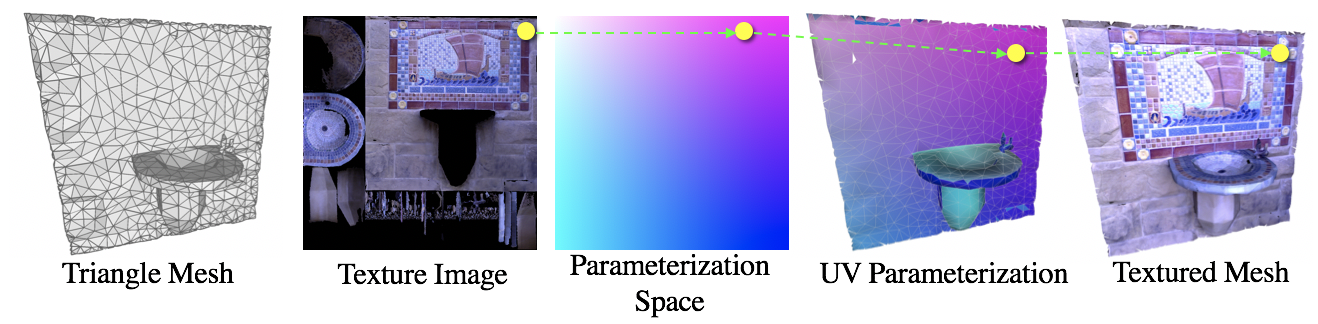
\includegraphics[width=\linewidth]{intro/texture-represent.png}
    \caption{Textured mesh representation in the computer. The geometry information is stored as a triangle mesh. The color information is stored as a surface texture with a UV parameterization for all vertices and a texture image stored in the parameterization space.}
    \label{fig:intro-texture-represent}
\end{figure}
We focus on the surface texture processing -- reconstructing and understanding the surface texture based on commodity RGB-D cameras.

By reconstruction, we aim at producing high-quality texture from inaccurate and low-quality scanning data. The wide availability of consumer range cameras has spurred extensive research in geometric reconstruction of real-world objects and scenes, with state-of-the-art 3D reconstruction approaches now providing robust camera tracking and 3D surface reconstruction~\cite{newcombe2011kinectfusion,izadi2011kinectfusion,whelan2015elasticfusion,dai2017bundlefusion}. However, producing a photorealistic textured mesh of real-world environments requires not only geometric reconstruction but also high-quality color reconstruction.
Unfortunately, due to noisy input data, poorly estimated surface geometry, misaligned camera parameters, unmodeled optical distortions, and view-dependent lighting effects,  aggregating multiple real-world images into high-quality, realistic surface textures is still a challenging problem. We aim at addressing this problem by minimizing color inconsistency or jointly optimizing the texture with a learned metric, as described in section~\ref{intro:texture-recon}.

While our deep metric can be implemented with an image convolutional neural network (CNN) as a widely-studied deep learning technique, one followup in this thesis is to directly apply a CNN in the texture domain of the 3D surface.
%
The advantage of applying CNN operator on 3D data over 2D images is obvious: convolutions directly operated in 3D data are relatively unaffected by view-dependent image effects, such as perspective, occlusion, lighting, and background clutter.
%
There has been a lot of recent works on the semantic segmentation of 3D data using 3D CNN. However, the resolution of current 3D representations is generally quite low (2cm is typical), and so the ability of 3D CNNs to discriminate fine-scale semantic patterns is usually far below their color image counterparts \cite{long2015fully,he2017mask}.
%
We believe a 2D CNN applied in the texture domain of the 3D surface can address the above issue, and the key challenge is to obtain a consistent and canonical surface parameterization that maps the 3D surface into a 2D space where 2D convolutions can apply.
%
We find that this challenge is related to the seamless surface parameterization problem in the computational geometry community. While this problem has been studied for more than a decade, the existing state-of-the-art method formulated as a mixed-integer programming problem (NP-hard), where an effective and robust solution is unavailable.
%
We reformulate the problem and obtain a robust and efficient seamless parameterization for the geometry of a complex 3D environment (section~\ref{intro:param}).


With the surface parameterization, we propose a surface convolution operator that extracts effective features in the parameterization space (section~\ref{intro:texture-learn}).
%
Specifically, we apply our convolution operator in our well-defined geodesic neighborhood where each point is locally parameterized with a 2D coordinate based on our seamless parameterization.
%
We make our novel convolution operator four-way rotationally symmetric to canonicalize the feature extraction with the existence of orientation singularities in the parameterization.
%
Our surface convolution is a 2D operator that effectively handles, and thereby outperforming other less efficient dense 3D convolution operators.
%
We find that the surface parameterization serves as not only a basis for surface convolution operators to apply but also useful information that is highly-correlated and learnable from the color signals. Therefore, we create a dataset with pairs of RGB images and pre-computed 3D canonical frames from the scanning data and train a neural network to predict frames from color signals. Our network enables various applications including surface normal estimation, feature matching and augmented reality (section~\ref{intro:frame}).

In summary, this thesis addresses the surface texture processing problem from the perspective of texture reconstruction (section~\ref{intro:texture-recon}) and texture understanding. We further identify the texture understanding problem as the surface parameterization problem (section~\ref{intro:param}) and learning methods based on it (section~\ref{intro:understand}). We summarize the contribution of the thesis in section~\ref{intro:contribution}.

\section{Texture Reconstruction}
\label{intro:texture-recon}
This section discusses our motivation and approaches for texture reconstruction. We discuss the related works about texture reconstruction is section~\ref{related:texture-recon} and introduce the technical details of our approaches including \textit{3DLite}~\cite{huang20173dlite} and \textit{Adversarial Texture Optimization}~\cite{huang2020adversarial} in chapter~\ref{chapter:texture-recon}.

\paragraph*{Motivation} RGB-D scanning has made rapid advances in recent years with the introduction of commodity range sensors, such as the Microsoft Kinect, Intel RealSense, or Google Tango. In this scenario, the textured mesh can be produced by fusing depth images into the geometry and color images into the surface texture.
State-of-the-art online and offline 3D geometry reconstruction methods now allow remarkable capture and digitization of a variety of real-world environments, with faithful geometric fidelity~ \cite{newcombe2011kinectfusion,izadi2011kinectfusion,chen2013scalable,niessner2013real,choi2015robust,dai2016bundlefusion}.
Although the intended applications of these methods cover a variety of gaming, virtual reality, and augmented reality scenarios, the quality of the resulting 3D models remains far from the caliber of artist-modeled content.
In particular, current reconstructions still suffer from noise, oversmoothing, and holes, rendering them inadequate for use in production applications. Therefore, both the geometry and the texture from the 3D reconstruction are problematic for the real applications.

\begin{figure}
    \centering
    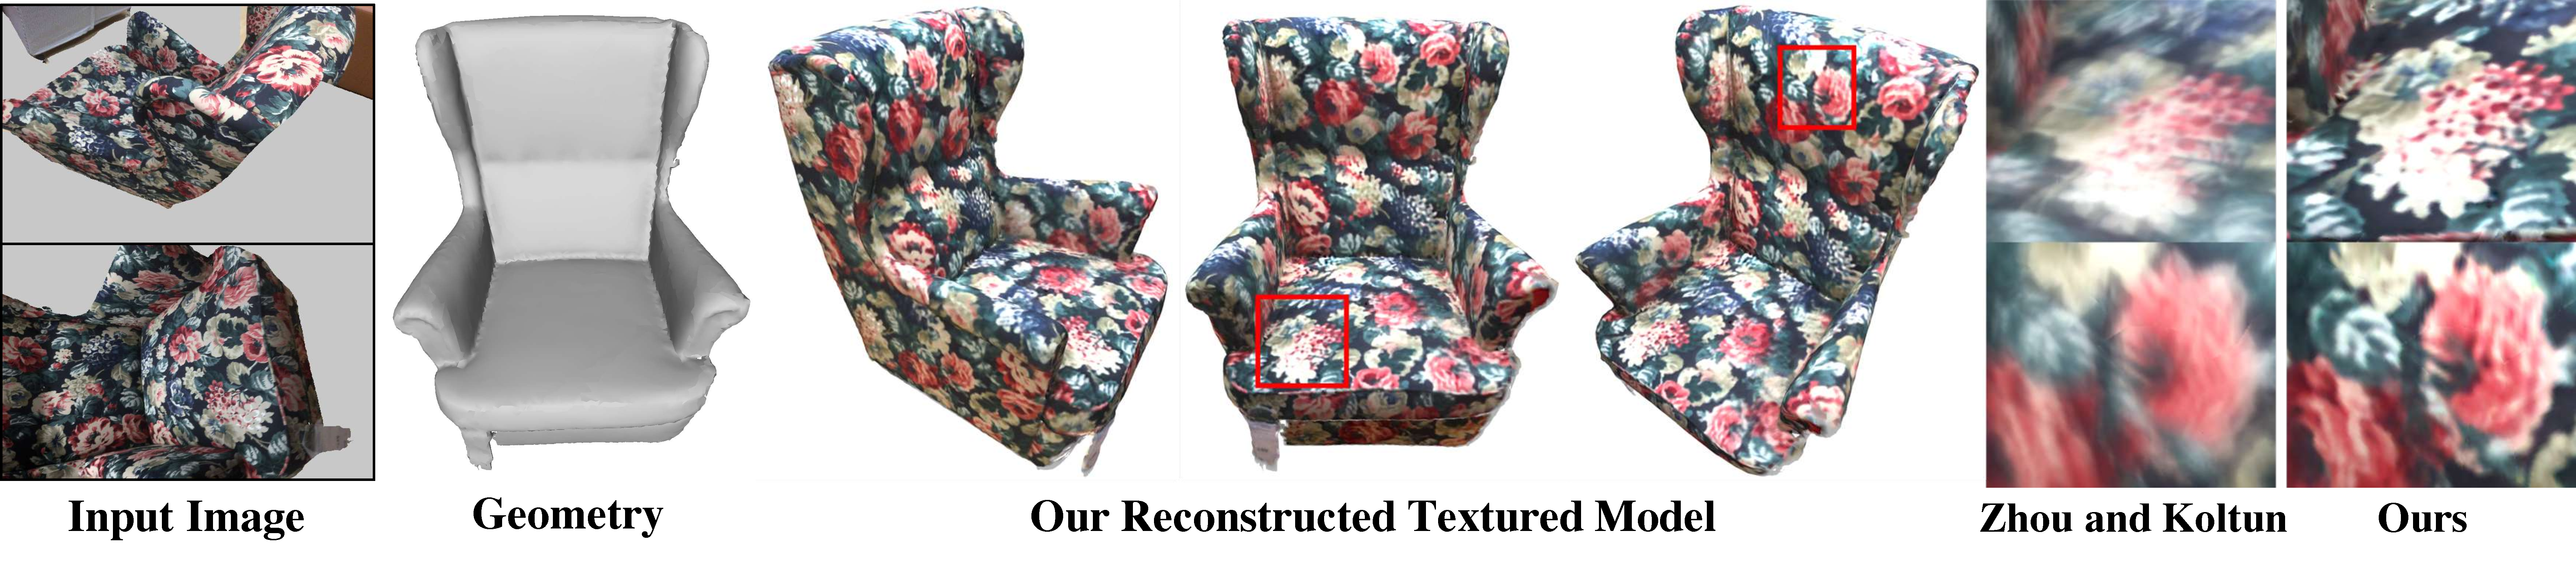
\includegraphics[width=\textwidth]{texturegen/figures/teaser-n.pdf}
    \caption{Our goal is to reconstruct high-quality textures from the 3D scan with aligned input images. Traditional methods optimize for a parametric color map to reduce misalignment error (Zhou and Koltun~\cite{zhou2014color}). We seek better color consistency optimization and view aggregation method, and further derive a flexible texture optimization framework based on a learned metric that is robust to common scanning errors.}
    \label{fig:toptim-teaser}
\end{figure}
From the graphics perspective, we observe that the surface textures are more important to visual perception than geometry; for instance, many video games make use of techniques such as billboarding or bump mapping~\cite{decoret1999multi}
to achieve high-detail visuals at low cost, with an almost imperceptible difference to using accurate geometry. Therefore, accurate geometric reconstruction is heavy and unnecessary, while light-weighted approximations of the scanning geometry with artifact-free primitives or CAD models are favored for interactive applications including gaming and virtual/augmented reality. 
Thus, our works assume inaccurate geometries from reconstructed from the scan or even further approximated with light-weight primitives and CAD models and focus on the high-quality texture mapping given the input as the RGB images and misaligned geometry as shown in figure~\ref{fig:toptim-teaser}.

High-quality texture reconstruction is a challenging problem. The color quality of existing 3D reconstruction methods often suffers from artifacts due to motion blur and rolling shutter from commodity color cameras. 
This is compounded by oversmoothing and camera pose micro-misalignments due to popular reconstruction techniques.
For instance, the seminal volumetric fusion work~\cite{curless1996volumetric} is commonly used to generate a 3D model from input RGB-D frames by performing a weighted average over projected depth and color observations.
While effectively regularizing out noise, this also results in oversmoothed geometry and color.
Additionally, since camera poses are computed from imperfect color and noisy, relatively low-quality depth, they often suffer from micro-drift, which further exacerbates resulting visual artifacts such as ghosting and oversmoothing. To overcome these problems, various approaches have been developed to optimize color textures using models to adjust camera poses~\cite{zhou2014color}, distort images~\cite{bi2017patch,zhou2014color}, and balance colors \cite{zhou2014color}.  However, these prior approaches are not expressive enough and/or their optimization algorithms are not robust enough to handle the complex distortions and misalignments commonly found in scans with commodity cameras -- and therefore they fail to produce high-quality results for typical scans as shown in the results from Zhou and Koltun~\cite{zhou2014color} in Figure~\ref{fig:toptim-teaser}.

To address these issues, we propose two approaches from different perspectives. The first approach~\cite{huang20173dlite} seeks better color consistency optimization and view aggregation by optimizing an explicit parametric models. The second approach~\cite{huang2020adversarial} further derives a flexible texture optimization framework based on a learned metric that is robust to common scanning errors (right side of Figure~\ref{fig:toptim-teaser}).
 
\paragraph*{Geometry Priors}
Our first approach, \emph{3DLite}~\cite{huang20173dlite}, generates lightweight, complete, CAD-like models of large-scale indoor scenes before we reconstruct high-quality textures.
%
We take as input an RGB-D video sequence from a handheld commodity sensor and first reconstruct the scene with existing 3D reconstruction methods.
Since we aim to generate complete scenes and sharp, clean textures, we employ a primitive-based abstraction to represent the scanned environments.
In particular, we use plane primitives, as planes facilitate texture mapping as well as scene completion through extrapolation, thus generating a denoised geometric representation of the scene.
%
We first optimize for these primitives under a Manhattan assumption, since man-made environments are often designed in such highly structured fashion.
To complete the scene geometry in occluded regions, we formulate a new hole-filling approach by extrapolating the planar primitives according to unknown space as seen by the camera trajectory.
That is, we respect the known empty space in the scene and only fill holes in regions unseen by the camera.
This generates a complete geometric representation of the scene.
%
Our second approach, \emph{Adversarial Texture Optimization}~\cite{huang2020adversarial}, learns a deep-metric that tolerates complex misalignment between image observations and the target geometry. Therefore, we can replace the scanning geometry with clean human-created CAD models with geometry misalignments but still perform decent texture optimization.

\paragraph*{Parametric Texture Optimization}
Our first approach~\cite{huang20173dlite} performs a novel texture optimization to map the scene geometry with sharp colors from the input RGB data.
Since camera poses estimated from noisy RGB-D data are prone to micro-drift, our texture optimization step solves for refined rigid and non-rigid image alignments, optimizing for photo-consistency using both sparse color and dense geometric information.
%
Zhou \textit{et al.}~\cite{zhou2014color} optimize purely for a dense energy term remains sensitive to initial poses and easy to end up in local minima. Therefore, we build upon them and employ a sparse-to-dense optimization, using sparse color features and geometric primitive constraints to help reach the basin of convergence of the dense photo-consistency energy.
%
To mitigate the effects of motion blur and auto-exposure, we perform an exposure correction and select and stitch together only the sharpest regions of the input RGB images, obtaining globally consistent, sharp colors. While existing methods reduce blurriness artifacts caused by average aggregation with single view selection~\cite{dessein2014seamless}, we further take pixel sharpness into consideration in the existence of motion blur. We select the best view for each region to balance the visual sharpness and color consistency of boundaries between neighboring regions with different views selected, which is modeled as a multi-label graph-cut problem~\cite{boykov2001fast}.

\paragraph*{Adversarial Metric for Texture Optimization}
Prior approaches depend on explicit models and color consistency optimization, and are not expressive enough and/or their optimization algorithms are not robust enough to handle the complex distortions and misalignments commonly found in scans with commodity cameras.

\begin{figure}
    \centering
    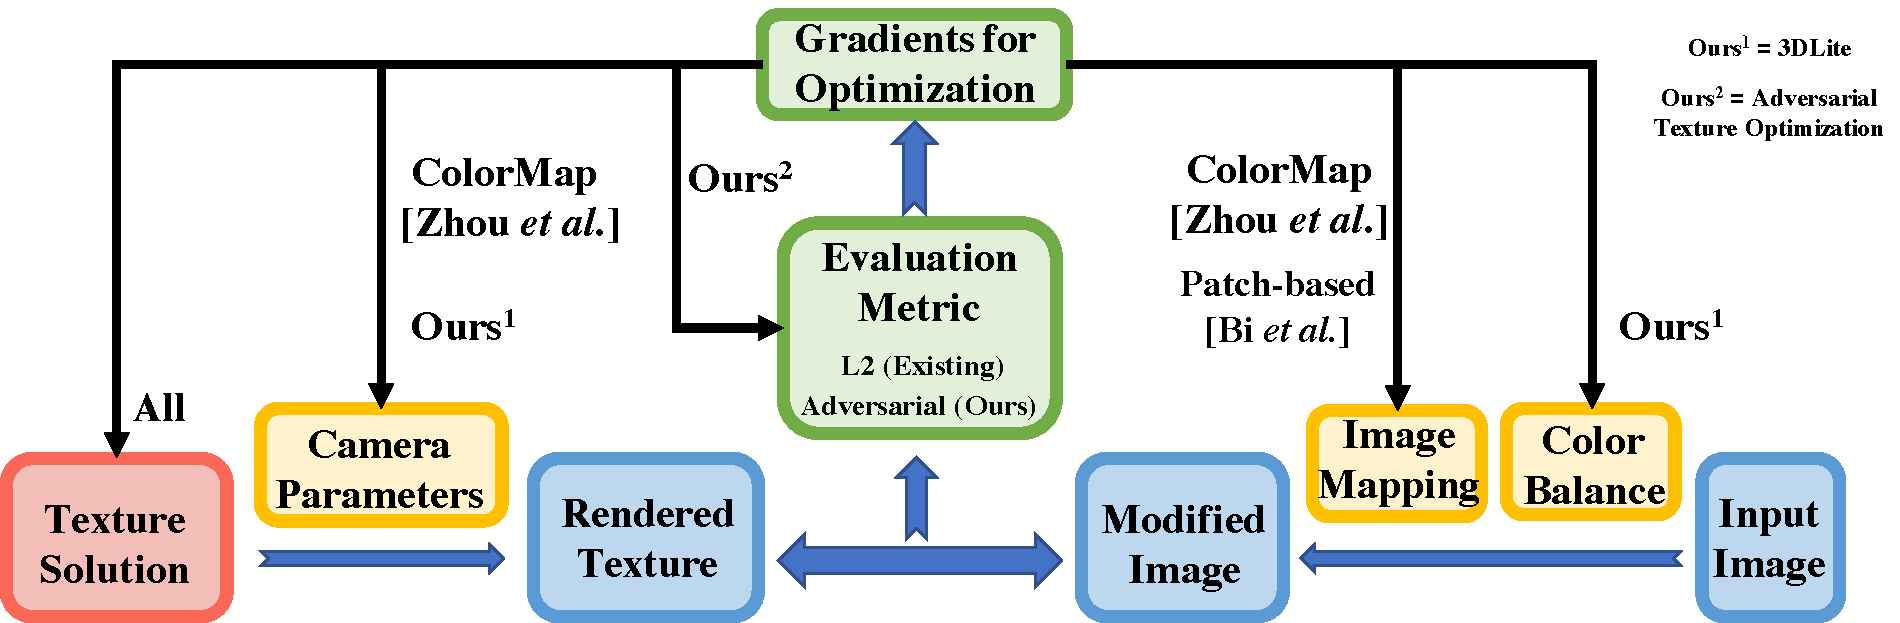
\includegraphics[width=\linewidth]{texturegen/figures/concept.pdf}
    \caption{All methods target at optimizing a texture solution. Existing methods optimize the texture jointly with camera parameters~\cite{zhou2014color,huang20173dlite}, image mapping~\cite{zhou2014color,bi2017patch} or color balance~\cite{huang20173dlite}. Instead, we jointly solve texture with an adversarial evaluation metric to tolerate the errors.}
    \label{fig:toptim-concept}
\end{figure}
To address these issues, our second approach~\cite{huang2020adversarial} proposes a flexible texture optimization framework based on a learned metric that is robust to common scanning errors.
% the scanning errors tuned separately for each individual scan. 
 The key idea behind our approach is to account for misalignments in a {\em learned objective function} of the texture optimization.   
 Rather that using a traditional object function, like $L1$ or $L2$, we learn a new objective function (adversarial loss) that is robust to the types of misalignment present in the input data.  This novel approach eliminates the need for hand-crafted parametric models for fixing the camera parameters \cite{zhou2014color,huang20173dlite} or image mapping \cite{bi2017patch,zhou2014color} or color balance \cite{huang20173dlite} (bottom row of Figure~\ref{fig:toptim-concept}) and replaces them all with a learned evaluation metric (green box in Figure~\ref{fig:toptim-concept}).   As such, it adapts to the input data.
 
Inspired by the success of adversarial networks in image synthesis~\cite{goodfellow2014generative}, we propose to use a learned conditional discriminator to serve our {\em objective function} and jointly optimize the color texture of a reconstructed surface with this discriminator.
The condition is a captured image $I_A$ from the source view $V_A$, and the query is either (i) ``real:'' a second captured image $I_B$ (from an auxiliary view $V_B$) projected onto the surface and then rendered back to $V_A$, or (ii) ``fake:'' an image of the optimized synthetic texture rendered to view $V_A$. By optimizing the surface texture while jointly training this conditional discriminator, we aim to produce a texture that is indistinguishable from reprojections of captured images from all other views.  
%
During the optimization, the discriminator learns invariance to the misalignments and distortions present in the input dataset, while recognizing synthetic artifacts that do not appear in the real images, like local blurs and seams.  The synthesized textures optimized to fool the discriminator appear more realistic than in previous approaches.

Our experiments show that our adversarial optimization framework produces notably improved performance compared to state-of-the-art methods, both quantitatively on synthetic data and qualitatively on real data. 
Moreover, since it tolerates gross misalignments, we are able to generate realistic textures on CAD models which have been only roughly aligned to 3D scans, in spite of large mismatches in surface geometry. 
This opens up the potential to produce CAD models with realistic textures for content creation.

\section{Surface Parameterization}
\label{intro:param}
While our adversarial texture optimization~\cite{huang2020adversarial} uses image convolution, it is more straightforward to perform convolution directly in the parameterized texture space for texture understanding. This section discusses the seamless surface parameterization as the necessary step towards texture understanding, and formulate it as a quadrangulation problem. We discuss the related works in section~\ref{related:param} and the technical details for our quadrangulation method in chapter~\ref{chapter:param}.

\paragraph*{Motivation} For adversarial texture optimization~\cite{huang2020adversarial}, we apply the 2D convolution to learn a misalignment-tolerant metric in the image space. A natural followup is to extract the features for the surface texture by directly applying the 2D convolution in the texture domain. While convolutions directly operated in 3D data are relatively unaffected by view-dependent image effects compared to image-based convolutions, the resolution of current 3D representations is generally quite low given higher dimensions of the data. Fortunately, texture signals lie on the surface instead of the whole 3D volume. It opens the opportunity for us to parameterize the surface using a 2D domain and apply a 2D convolution in the parameterization space. We observe the key difference between 2D images and 3D surfaces is that the image coordinate system serves as a consistent global definition of how the 2D domain is parameterized, while there is no global consistent definition of surface parameterization in 3D.

 \begin{figure}
  \centering
  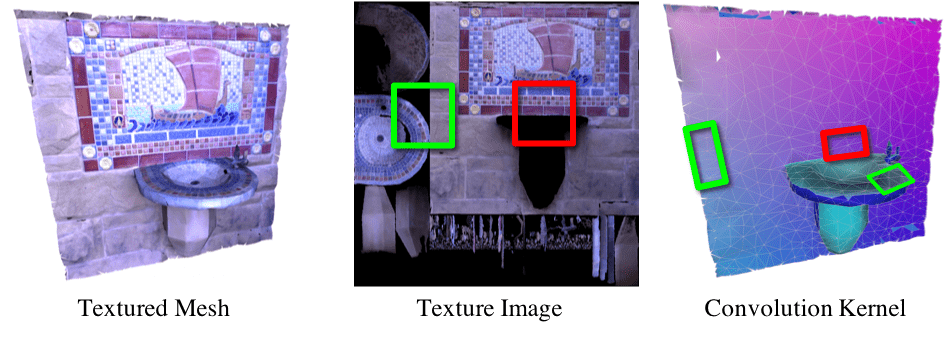
\includegraphics[width=0.8\linewidth]{intro/uvconv.png}
  \caption{Limitation of convolutions with a general UV parameterization. The convolution applied to the texture image incorrectly aggregates disconnected regions (green) and incorporates unexpected boundaries (red).}
  \label{fig:intro-uv-param}
\end{figure}
For example, the most straightforward idea is to directly use general UV parameterization. However, convolution applied to the texture image suffers can cause problems by breaking the connectivity information in the 3D. As shown in figure~\ref{fig:intro-uv-param}, the green convolution kernel incorrectly aggregates disconnected regions of the mesh. Additionally, the red convolution kernel in the texture image reaches the boundaries, while ideally, this should not happen since the center is far from the surface boundary.
 \begin{figure}
    \centering
     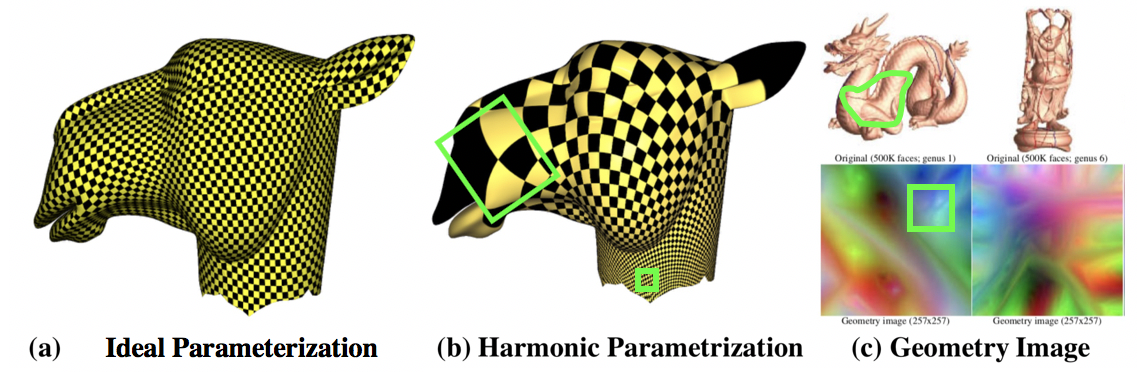
\includegraphics[width=0.8\linewidth]{quadriflow/param.png}
     \caption{(a) With an ideal parameterization, we can get the surface parameterization aligned with shape features with negligible distortion. (b) Harmonic parameterization leads to high distortion in the scale. (c) Geometry images~\cite{gu2002geometry} result in high distortion in the orientation.}
     \label{fig:intro-quadriflow-param}
 \end{figure}
Other well-known parameterization methods can also cause different problems. In figure~\ref{fig:intro-quadriflow-param}, the receptive field of the convolution (marked as green edges) can have significant different scales with harmonic parameterization or irregular neighborhoods with geometry images~\cite{gu2002geometry}. We argue that an ideal parameterization for convolution should be regular, uniform and seamlessly connected. In this case, the receptive field is regular and canonicalized with the same shape and size. Such a parameterization is shown in figure~\ref{fig:intro-quadriflow-param}(a), where the surface is seamlessly parameterized and visually looks like a uniform-scale quadrilateral mesh. Therefore, to tackle the texture convolution problem, we first build a robust and scalable quadrangulation algorithm to convert a general triangle mesh as a quadrilateral mesh as \textit{Quadriflow}~\cite{huang2018quadriflow}.

\paragraph*{Orientation and Singularity} State-of-the-art algorithms for quadrilateral surface meshing typically compute, as a first step, an \emph{orientation field} that assigns local coordinate axes to some points on the input surface \cite{knupp1995mesh,ray2006periodic,kalberer2007quadcover,bommes2009mixed}. The {\em Instant Field-Aligned Meshes} \mbox{algorithm} of Jakob et al.~\cite{jakob2015instant} subsequently computes a \emph{position field} that assigns local coordinates %(in the frame of the local coordinate axes)%
to those points. The orientation field determines the directions of the edges of a quadrilateral mesh, and the position field determines where the mesh vertices are placed. Ideally, both fields should vary smoothly over the surface, while obeying constraints that help to align the mesh with the sharp edges and the curvature of the object.

Both types of fields can have irregularities called \emph{singularities}. If the fields are defined continuously over the surface, a singularity is a region where one of the fields is not locally smooth.
The pitfall of these singularities is that the quad mesh subsequently produced is likely to have an \emph{irregular vertex}---a vertex whose valence is not 4---near the singularity. 
Unfortunately, irregular vertices can cause problems for applications; for instance, they cause unsightly visual artifacts in Catmull--Clark subdivision, or additional work for an artist to edit a model. In our texture understanding scenario, such irregularity means that our convolution kernels are highly distorted or not canonically oriented near the singularity positions.

Algorithms that rely purely on local mesh computations are fast, but they produce meshes with many singularities. It is possible to modify the fields to move singularities and sometimes even to eliminate them; but eliminating a singularity
usually involves merging pairs of singularities located all around the geometry, which is ``nonlocal.'' 
A global view of quad meshing taken by Bommes et al.~\cite{bommes2009mixed}, who cast the problem of seamless global parametrization as a mixed-integer constrained optimization problem (MIP).
The method produces quadrilateral surface meshes of very high quality, but it is slow and it does not scale well to large meshes. By contrast, the much more efficient Instant Meshes algorithm of Jakob et al.~\cite{jakob2015instant} uses local smoothing operators to compute an orientation field and a position field quickly. Their method is scalable and produces high-quality quad-dominant meshes without much distortion. However, it may produce singularities in the position field in addition to singularities in the orientation field.

\paragraph*{Our Formulation} We present \emph{QuadriFlow}~\cite{huang2018quadriflow}, a scalable, robust algorithm for automatic quad meshing that builds upon Instant Meshes but uses a global method to remove all the singularities from the position field.
We do not change the orientation field, which typically has many fewer singularities. Our method solves a minimum cost network flow problem as a subproblem, for which efficient algorithms are available. The speed and reliability of our algorithm can enable designers to work on a modeling task interactively and extract a quad mesh in less than a second for tens of thousands of faces, and enable physical simulations to perform per-timestep remeshing updates. Our current implementation is a \emph{remeshing} algorithm, meaning that its input is a triangular mesh of the input surface (like many other quad meshing algorithms), though it could be modified to take a point cloud input as Instant Meshing does.

We view singularity-free position field computation as a globally constrained optimization problem.
Unlike Bommes et al., we do not solve the problem by mixed-integer programming. Instead, we split it into three stages.
\begin{itemize}
\item Compute the orientation and position fields just as Jakob et al.\ do, without enforcing additional constraints.
\item Enforce our constraints by modifying only the integer variables of the position field, changing the integers as little as possible.
\item Re-optimize the continuous variables of the position field with the integer variables held fixed.
\end{itemize}
The third stage is not difficult, requiring the solution of a linear system. Our main contribution is a fast and effective method for the second, largely combinatorial stage. Because of the regularity constraints, the second stage is a mixed-integer programming problem, for which it is NP-hard to find an optimal solution, but we can obtain good approximate solutions in practice. We reduce the problem to an integer linear program (ILP). We approximate the ILP as an easier \emph{minimum cost network flow} (MCF) problem, which can be solved in polynomial time~\cite{klein1967primal}. We further improve efficiency by a multi-resolution algorithm. To enforce consistent triangle orientations (no inverted triangles), we impose a set of quadratic inequality constraints. We are able to satisfy most of these constraints through simple greedy edge contractions; we find we can satisfy most of the remaining difficult ones by locally solving a small boolean satisfiability problem (SAT).

By replacing the MIP solver with an MCF solver that globally reduces the number of singularities, plus edge contractions and an SAT solver that locally impose triangle orientation constraints, we obtain a scalable quad remesher that produces many fewer singularities than Instant Meshes, often by a factor of four, while being much faster than the method of Bommes et al. QuadriFlow remeshes a one-million triangle mesh in 5 seconds, which is comparable to the interactive method of Ebke et al.~\cite{ebke2016interactively}. Our meshes have less distortion compared to other global methods, and rarely suffer from nonmanifold structure or holes, thanks to the consistent orientation constraints. In a test on 17,000$+$ surfaces created from ShapeNet~\cite{chang2015shapenet}, QuadriFlow robustly removed all the singularities from every discrete position field.
 
\section{Texture Understanding}
\label{intro:understand}
With the powerful seamless parameterization of the surface, we are able to explore the texture understanding problem. This thesis explores the semantic understanding problem with the parameterized textures as well as the 3D frame understanding given the RGB images.

\subsection{Semantics from Texture}
\begin{figure}
    \begin{center}
        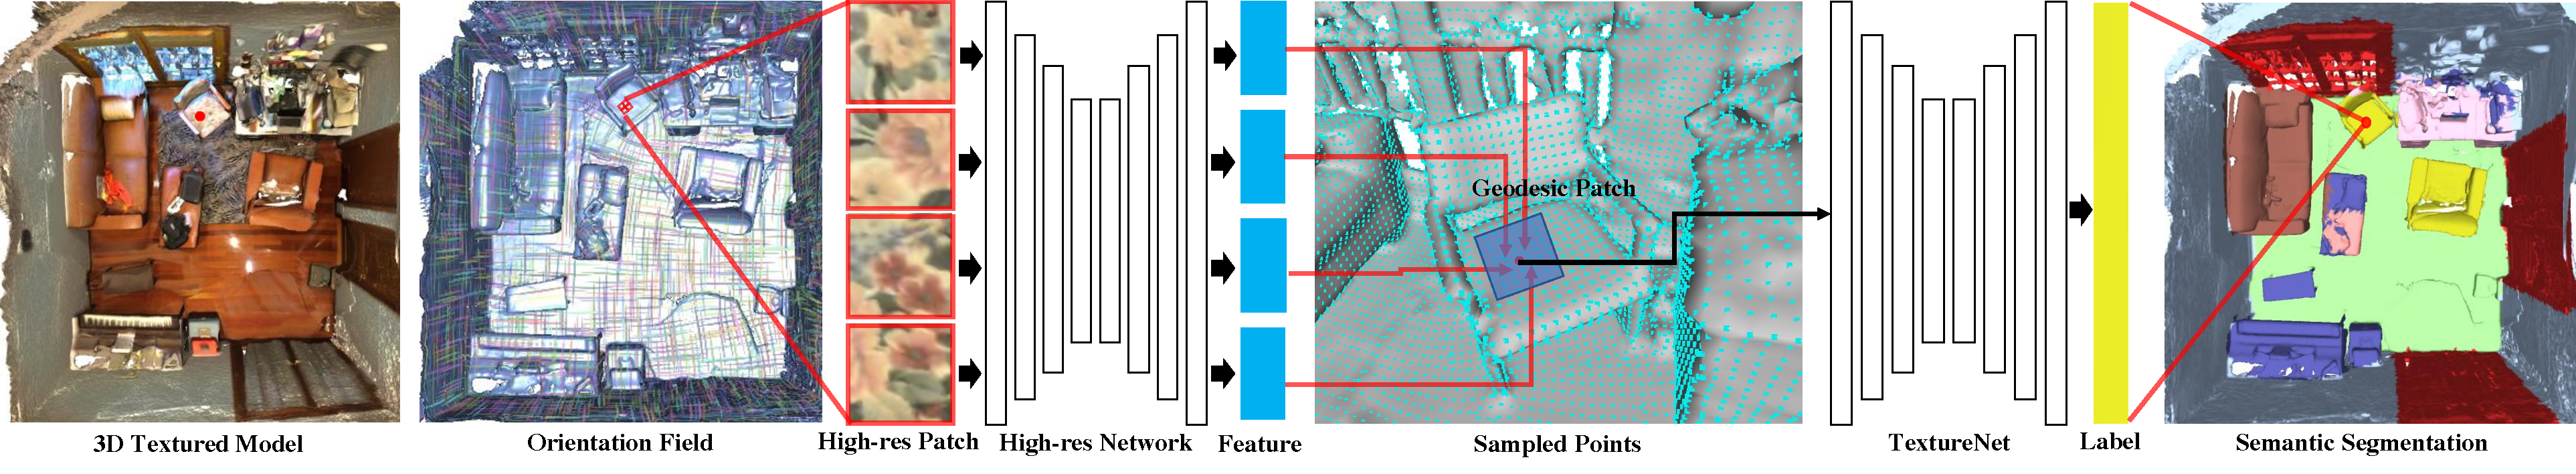
\includegraphics[width=\linewidth]{texturenet/teaser/teaser.pdf}
        \caption{TextureNet takes as input a 3D textured mesh.  The mesh is parameterized with a consistent 4-way rotationally symmetric (4-RoSy) field, which is used to extract oriented patches from the texture at a set of sample points.   Networks of 4-RoSy convolutional operators extract features from the patches and used for 3D semantic segmentation.}
        \label{fig:texturenet-teaser}
    \end{center}    
\end{figure}
\label{intro:texture-learn}
Given the robust seamless surface parameterization, we are able to explore the semantic understanding from the texture signals. We design TextureNet~\cite{huang2018texturenet} as a neural network architecture (figure~\ref{fig:texturenet-teaser}) to extract features from high-resolution signals associated with the 3D surface meshes (e.g., color texture maps).
There has been a lot of recent work on the semantic segmentation of 3D data using convolutional neural networks (CNNs).  Typically, features extracted from the scanned inputs (e.g., positions, normals, height above ground, colors, etc.) are projected onto a coarse sampling of 3D locations, and then a network of 3D convolutional filters is trained to extract features for semantic classification -- e.g., using convolutions over voxels \cite{wu20153d,maturana2015voxnet,qi2016volumetric,song2017semantic,dai2017scannet,dai2018scancomplete}, octrees \cite{riegler2017octnet}, point clouds \cite{qi2017pointnet,qi2017pointnet++}, or mesh vertices \cite{masci2015geodesic}.  The advantage of these approaches over 2D image-based methods is that convolutions operate directly on 3D data, and thus are relatively unaffected by view-dependent image effects, such as perspective, occlusion, lighting, and background clutter.   However, the resolution of current 3D representations is generally quite low (2cm is typical), and so the ability of 3D CNNs to discriminate fine-scale semantic patterns is usually far below their color image counterparts \cite{long2015fully,he2017mask}.

To address this issue, we propose a new convolutional neural network, \emph{TextureNet}~\cite{huang2018texturenet}, with a 2D convolution kernel that extracts features directly from high-resolution signals associated with 3D surface meshes.  Given a map that associates high-resolution signals with a 3D mesh surface (e.g., RGB photographic texture), we define convolutional filters that operate on those signals within domains defined by geodesic surface neighborhoods.   This approach combines the advantages of feature extraction from high-resolution signals (as in \cite{dai20183dmv}) with the advantages of view-independent convolution on 3D surface domains (as in \cite{tatarchenko2018tangent}).

During our investigation of this approach, we had to address several research issues, the most significant of which is how to define geodesic neighborhoods of a mesh.   One approach could be to compute a global UV parameterization for the entire surface and then define convolutional operators directly in UV space; however, that approach may induce significant deformations due to flattening, not always follow surface features, and/or produce seams at surface cuts.  Another approach could be to compute UV parameterizations for local neighborhoods independently; however, then adjacent neighborhoods might not be oriented consistently, reducing the ability of a network to properly learn orientation-dependent features.   Instead, we compute a 4-RoSy (four-fold rotationally symmetric) field on the surface using QuadriFlow~\cite{huang2018quadriflow} and define a new 4-RoSy convolutional operator that explicitly accounts for the 4-fold rotational ambiguity of the cross-field parameterization. A 4-RoSy (four-way rotationally symmetric) field is a configuration of 4 orthogonal tangent directions associated with each vertex in the shape of a cross that varies smoothly over the mesh surface.  Since the 4-RoSy field from QuadriFlow has no seams, aligns to shape features, induces relatively little distortion, has few singularities, and consistently orients adjacent neighborhoods (up to 4-way rotations), it provides an attractive trade-off between distortion and orientation invariance.

Results on 3D semantic segmentation benchmarks show an improvement of the 4-RoSy convolution on surfaces over alternative geometry-only approaches (by 6.4\%), plus significantly further improvement when applied to high-resolution color signals (by 6.9-8.2\% ).  With ablation studies, we verify the importance of the consistent orientation of a 4-RoSy field and demonstrate that our sampling and convolution operator works better than other alternatives.

\subsection{FrameNet: Canonical Frame Understanding from RGB Images}
\label{intro:frame}
 \begin{figure}
    \centering
    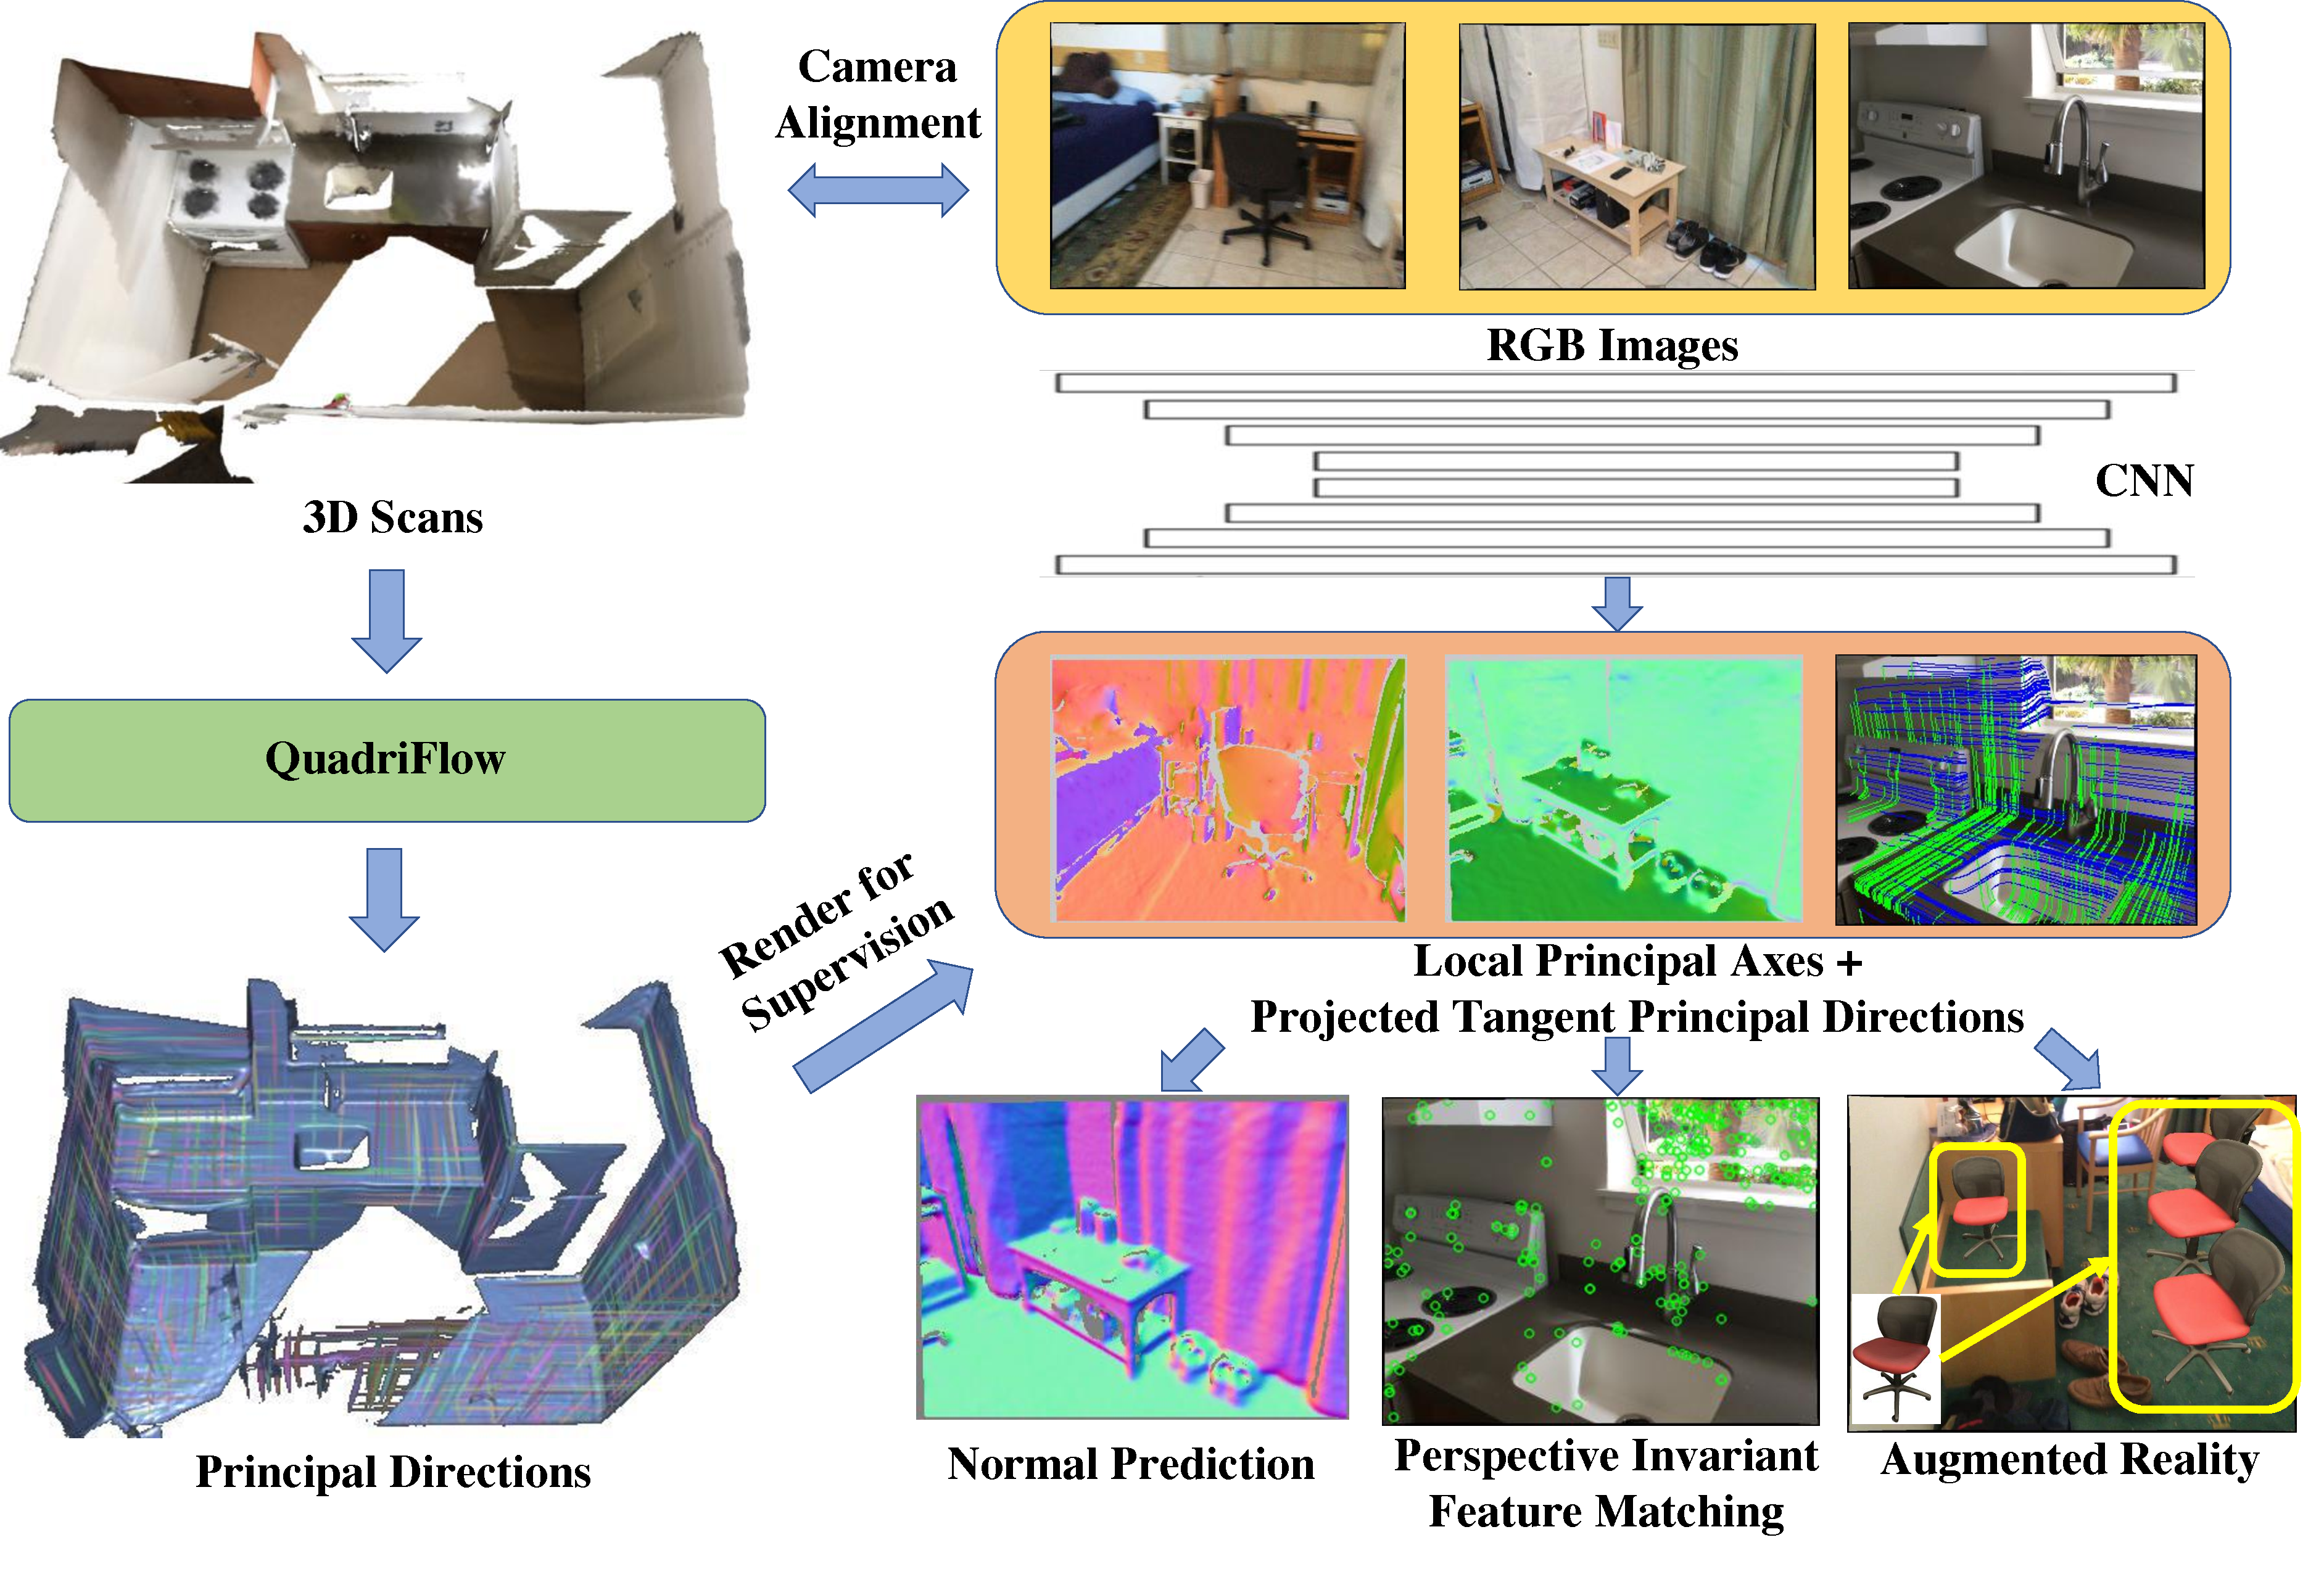
\includegraphics[width=0.75\linewidth]{FrameNet/graph/teaser.pdf}
    \caption{We propose the novel task of predicting dense 3D \cframe{} from a single RGB image. We compute the frames from reconstructed meshes using QuadriFlow and render them to images to supervise the task.  We train a network that predicts all directions of the frames jointly.  We find that predicted tangents provides better surface normals, and are useful for applications like feature matching and augmented reality.}
    \label{fig:framenet-teaser}
    \vspace{-0.1in}
\end{figure}
The seamless surface parameterization is itself an important feature that is strongly correlated with the RGB signals. The edge orientations of our quad mesh are aligned with the tangent principal directions. At the same time, we observe that each pixel in an image is the projection of a small surface region in the underlying 3D geometry, where a canonical frame can be identified as represented by three orthogonal axes, one along its normal direction and two along tangent principal directions specified by the quad edges. Therefore, we introduce FrameNet~\cite{framenet} as a novel image-to-3D task: dense 3D \cframe{} estimation from a single image (figure~\ref{fig:framenet-teaser}).

In fact, the image-to-3D tasks have made great progress in recent years.  For example, monocular depth estimation~\cite{shelhamer2015scene,li2017two,xu2017multi,wang2018adaptive,fu2018deep} and surface normal prediction~\cite{eigen2015predicting,wang2015designing,bansal2016marr,qi2018geonet} have improved dramatically.  There are many applications for these tasks in scene understanding and robot interaction.
%
The main challenge in this domain is choosing an appropriate representation of 3D geometry to predict.  Zhang~\textit{et al.}~\cite{zhang2018deep} predict dense surface normals and then use geometric constraints to solve for depth with global optimization.  GeoNet~\cite{qi2018geonet} predicts both surface normals and depth and then passes them to a refinement network for further optimization.  These methods are clever in their use of geometric constraints to regularize dense predictions.   However, they infer only 2 of the 3 degrees of freedom in a 3D coordinate frame -- the rotation in the tangent plane around the surface normal is left unknown.  As such, they are missing 3D information critical to many applications.   For example, they cannot assist an AR system in placing a picture frame on a wall or a laptop on a table because they don't know the full 3D coordinate frame (including tangent directions) of the wall or table surfaces.

Our task instead requires predicting a full 3D coordinate frame defined by the surface normal {\em and two principal tangent directions} of the surface observed at every pixel in an RGB image.  We investigate this task for three reasons.   First, we expect that predicting principal tangent directions is easier than predicting normals because they are often aligned with observable patterns in surface textures (e.g., wood grains, fabric weaves, tile seams, etc.) and surface boundaries, which are directly observable in images.  Second, we expect that joint surface normal and tangent prediction is more robust than normal prediction alone due to the regularization provided by orthogonality constraints.  Third, we expect that predicting a full canonical 3D coordinate frame at every pixel is useful for many applications, such as augmented reality.

\cam{We have implemented an algorithm for this task in a supervised setting.   To acquire ``ground truth'' \cframe{}, we leverage data from RGB-D scanning datasets, like ScanNet~\cite{dai2017scannet}, which provide large sets of images posed within reconstructed 3D meshes.  
We compute \cframe{} on the meshes and render them to the RGB images to produce training data.  There are multiple choices for how to define the frames.  A simple approach would be to use Manhattan frames; however, they
reflect only the global scene orientation %(figure~\ref{fig:framenet-vis-direction}(a))
.   Instead, we compute locally consistent 4-RoSy \cframe{} that follow principal curvatures using the Quadriflow algorithm~\cite{huang2018quadriflow} %(figure~\ref{fig:framenet-vis-direction}(b))
.  We find that the surface tangent directions computed this way are consistent with image features and can be learned by a network from 2D data.}

\cam{The \cframes{} are fundamental 3D properties of a scene, as they imply the canonical transformation that maps the 3D surface to the image plane.  They provide not only the surface normal but also canonical tangent directions and their projections onto the image plane.  We show that predicting all these directions jointly can improve surface normal estimation, local patch description using SIFT features~\cite{lowe2004distinctive}, and allow the insertion of novel objects with correct orientation in augmented reality applications.}

\section{Contributions and Thesis Outlines}
\label{intro:contribution}
\begin{figure}
    \centering
    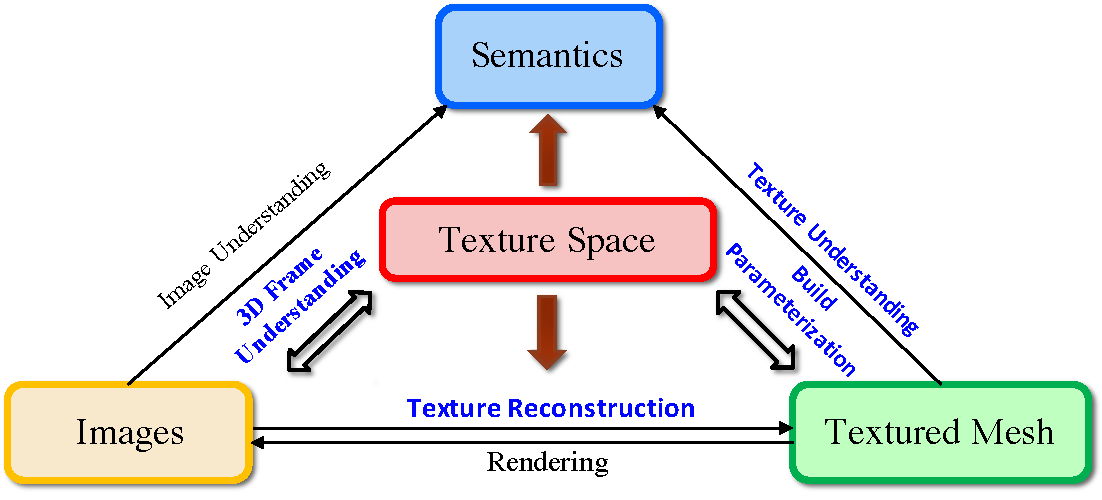
\includegraphics[width=0.75\linewidth]{intro/concept.pdf}
    \caption{Our works focus on surface texture processing to reconstruct and understand the environment. Our problems are marked using blue fonts. We reconstruct the surface texture based on images from the scans, build a seamless parameterization to create a texture space, and propose a texture convolution operator in such a space to understand the semantics. We further explore the understanding of the parameterization from the images.}
    \label{fig:intro-concept}
\end{figure}
This thesis mainly focuses on surface texture processing. In summary, figure~\ref{fig:intro-concept} illustrates the main components related to the surface texture. where our problems are marked using blue fonts. Basically, the surface texture has a strong relationship with the scanning images via rendering and reconstruction. We focus on reconstructing high-quality surface textures from images. We propose to construct the texture space using the seamless surface parameterization. This leads to an important representation that is helpful for texture understanding including the semantics understanding from parameterized textures and canonical frame understanding from images.

We discuss the related works in chapter~\ref{chapter:related}. Texture optimization is based on color consistency optimization~\cite{huang20173dlite} or joint adversarial metric optimization~\cite{huang2020adversarial}, as described in chapter~\ref{chapter:texture-recon}. For understanding, we first solve the fundamental surface parameterization problem~\cite{huang2018quadriflow} as explained in chapter~\ref{chapter:param}, and design a network with 2D convolution operators~\cite{huang2018texturenet} under the canonical surface parameterization (chapter~\ref{sec:texturenet}. Observing the correlation between surface parameterization and texture signals, we propose to learn canonical frames from RGB images~\cite{framenet} in chapter~\ref{sec:framenet}. Finally, we draw the conclusions and discuss about the future directions for surface texture processing in chapter~\ref{chapter:conclude}.

Overall, the contributions of this thesis include:
\begin{itemize}
    \item Identify the surface processing problem as to reconstruct the texture, parameterize the texture space and understand the texture.
    \item We propose \emph{3DLite} as an approach to produce high-quality surface textures on top of the lightweight planar geometry abstracted from the scan.
    \item We propose an \emph{adversarial texture optimization} method to produce photorealistic textures for approximate surfaces, even from misaligned images, by learning an objective function that is robust to scanning errors.
    \item We propose \emph{Quadriflow} as a scalable and robust quadrangulation algorithm that is solvable in polynomial time.
    \item Based on consistent local parameterizations from \emph{Quadriflow}, we design \emph{TextureNet} as a novel neural network for extracting features from high-resolution signals living on surfaces embedded in 3D.
    \item We observe the high correlation between surface parameterization from \emph{Quadriflow} and RGB signals on surface texture, and identify an important new 3D vision problem with a solution called \emph{FrameNet}: local canonical frame estimation from RGB images.
\end{itemize}


\chapter{Related Works}
\label{chapter:related}
In this chapter, we discuss the related works about texture reconstruction in section~\ref{related:texture-recon}. Surface parameterization is a classical problem in geometry processing community and is discussed in section~\ref{related:param}. We finally discuss related works about texture understanding,  including semantics understanding from 3D surface (section~\ref{related:texturenet}) and 3D geometry understanding from 2D image (section~\ref{related:framenet}).

\section{Texture Reconstruction}
\label{related:texture-recon}
\paragraph*{View Aggregation} Common texture reconstruction methods~\cite{izadi2011kinectfusion,zhou2014color} average projected input images to generate textures.  
To reduce blurriness artifacts, some approaches select a single or a few candidate views for each region \cite{dessein2014seamless}. Others formulate a multi-label selection energy minimization problem to minimize seam artifacts~\cite{lempitsky2007seamless,sinha2008interactive,velho2007projective,waechter2014let,huang20173dlite}. For instance, ~\cite{huang20173dlite} aims at selecting the best view for each region to balance the visual sharpness and color consistency of boundaries between neighboring regions with different views selected, which is modeled as a multi-label graph-cut problem~\cite{boykov2001fast}. Our method does not explicitly define the aggregation method, but implicitly aggregates colors from different views based on a learned adversarial metric.

\paragraph*{Parametric Color Optimization}
Several approaches have been proposed to improve the mapping of input images to textures with parametric models, %optimized to improve color consistency during view aggregation.  
leveraging both human supervision~\cite{franken2005minimizing,ofek1997multiresolution,pighin2006synthesizing,xu2019deep}, as well as automatic optimization~\cite{bernardini2001high,pulli2000surface}.  
Zhou \textit{et al.}~\cite{zhou2014color} propose to optimize a parametric model comprising camera poses and non-rigid grid deformations of input images to minimize an L2 color consistency metric. 
While these methods are able to fix small misalignments, their deformation models are often not expressive enough to handle many real-world distortions, particularly those due to largely approximate surface geometry. 
In contrast to a hand-crafted deformation model, we learn a distortion-tolerant adversarial loss.

\paragraph*{Patch-based Color Optimization}
Patch-based image synthesis strategies have been proposed for color texture optimization~\cite{bi2017patch}. Rather than non-rigid image warping, they re-synthesize the input image with the nearest patch search~\cite{simakov2008summarizing} to handle misalignments. 
However, general misalignment cannot be accurately modeled by translating patches, and the L2 loss is not robust to color, lighting or sharpness differences. 
Our method optimizes the discriminator to cover all these problems without requiring explicit re-synthesis.

\paragraph*{Color optimization for 3D reconstruction}  Various approaches have been developed to create a color map on a geometric model from multiple input images.
Several techniques use manually selected point correspondences to provide image-to-model registration~\cite{neugebauer1999texturing,ofek1997multiresolution,stamos20003d,rocchini1999multiple}. 
Given precisely registered pairs of color and depth, camera poses can be optimized for to maximize photo-consistency~\cite{johnson1999registration,pulli2000surface,pulli2005projective,bernardini2001high}. For 3D scanning using commodity-sensor data with various misalignments arising from coarse geometry and optical irregularities, Zhou and Koltun~\cite{zhou2014color} account for these issues by optimizing for both the rigid camera poses as well as non-rigid warping for each image to maximize dense photo-consistency. 
Bi et al.~\cite{PatchBasedTextureMapping} build on this work: they synthesize a set of photometrically consistent aligned color images to produce high-quality texture mapping even under substantial geometric inaccuracies.
We also build upon the approach of Zhou et al.~\cite{zhou2014color}; however, for our room-scale scenario, optimizing purely for a dense energy term remains sensitive to initial poses and easy to end up in local minima. 
Rather, we employ a sparse-to-dense optimization, using sparse color features and geometric primitive constraints to help reach the basin of convergence of the dense photo-consistency energy.

\paragraph*{Neural Textures}
Recently, neural rendering approaches have been proposed to synthesize a feature map on a surface that can be interpreted by a deep network to produce novel image views.  For instance, \cite{thies2019deferred} stores appearance information as high-dimensional features in a neural texture map associated with the coarse geometry proxy and decodes to color when projected to novel views.  \cite{sitzmann2019deepvoxels} stores the appearance information as high-dimensional features in volumes, and \cite{aliev2019neural} uses features stored with points. These methods rely on the representation power of generative networks at rendering times to obtain novel viewpoints, which limits their applicability in standard graphics pipelines.

\paragraph*{Texture Reconstruction with Geometry Priors}
The idea of approximating distant geometry through images called {\em impostors} was widely used in the image-based rendering literature~\cite{sillion1997efficient,decoret1999multi}. 
These images are in fact textured planes optimally positioned so as to generate approximately correct views from a range of viewpoints.
Image-based rendering has also been recently used in custom renderers with a geometry proxy, and achieved high-quality results using sparse DSLR input images \cite{hedman2016scalable}.

Since man-made environments are typically constructed in a highly-structured fashion, with an abundance or orthogonal and parallel planes, a Manhattan plane assumption can be exploited to facilitate tracking in indoor scenes, particularly in the case of RGB-D scanning, as depth information is directly available.
Many methods have been developed to incorporate planar information to improve camera tracking in 3D scanning scenarios.
Dou et al.~\cite{dou2012exploring} and Taguchi et al.~\cite{taguchi2013point} both incorporate various plane correspondences with feature point correspondences to improve tracking robustness. %, and can produce geometry-only simplified planar representations of the scanned scenes.
%Salas-Moreno et al.~\cite{salas2014dense} and Ma et al.~\cite{ma2016cpa} use planar detection and alignment to improve real-time SLAM performance.
Zhang et al.~\cite{zhang2015online} detect both planar structures and repeated objects to mitigate camera drift, achieving improved reconstruction quality in a KinectFusion-style framework.
In order to reduce sensitivity towards potential errors in initially detected structural correspondences, Halber and Funkhouser~\cite{halber2016fine} employ a hierarchical optimization approach incorporating planar relationship constraints with sparse features, enabling registration of very long RGB-D scanning sequences.

In addition to improving tracking robustness, Dzitsiuk et al.~\cite{dzitsiuk2016noising} use plane priors estimated directly on the  implicit signed distance field representation of the scene to further de-noise and complete the reconstruction, producing very stable geometry even during real-time updates.
Surface measurements near detected planes are replaced with the plane measurements to reduce noise, and plane geometry is extrapolated in unobserved space to fill holes.
Our approach similarly exploits planes as a clean geometric representation of a 3D scene which can be leveraged to complete 3D scenes; however, Dzitsiuk et al.~\cite{dzitsiuk2016noising} focus solely on geometry denoising and completion, whereas the goal of our proposed 3DLite is to create visually compelling models by generating high-quality texture for complete 3D models.


\section{Surface Parameterization}
\label{related:param}
\paragraph*{Robust Quadrangulations}
Robust quadrangulations based on local optimization have a rich literature. Bommes et al.~\cite{bommes2013quad} survey many existing methods for quad-mesh generation and processing.  Many methods transform a pre-existing triangle mesh into an all-quadrilateral mesh: Q-Morph~\cite{owen1999q} does so with an advancing front algorithm.  Blossom-Quad~\cite{remacle2012blossom} uses a perfect matching algorithm to pair triangles into quads with a global optimal solution. Velho and Zorin~\cite{velho20014} greedily identify the most eligible neighboring triangles to pair. SQuad~\cite{gurung2011squad} improves the representation of the connectivity of meshes, which can be applied to quadrangulation.  Since these methods are not guided by an orientation field, they have difficulty achieving global regularity or smoothness, and their meshes are often very irregular or have many singularities.  Spectral and Morse complex-based algorithms \cite{dong2006spectral,zhang2010wave,ling2014spectral} require no integer optimization but singularity control is hard for them.

\paragraph*{Orientation Fields}
An orientation field is a powerful tool to guide the edge directions in a quad mesh. Specifically, we use 4-way rotationally symmetric orientation fields~\cite{ray2008n,lai2010metric}. The target directions are derived from the principal curvatures~\cite{cohen2003restricted,cazals2005estimating}, but modified to vary smoothly. Smooth orientation fields are generated by optimizing a nonlinear energy function based on periodic functions~\cite{hertzmann2000illustrating,ray2009geometry} or a mixed-integer representation~\cite{ray2008n,bommes2009mixed}. However, these approaches may get stuck in poor local minima that have many singularities. Kn\"{o}ppel et al.~\cite{knoppel2013globally} propose a global optimization method to obtain better minima. Many approaches \cite{ray2008n,ray2009geometry,crane2010trivial,diamanti2014designing,jiang2015frame} integrate user interactions to help remove singularities.

\paragraph*{Field-algned Quadrangulations}
A direct approach to generating a quad mesh is to trace the curves in an orientation field~\cite{alliez2003anisotropic}, but it is difficult to control the sizes of the quads obtained that way. Lai et al.~\cite{lai2008incremental} directly optimize a triangle mesh to align its edges to an orientation field, then extract a quad mesh by pairing triangles. These methods are local, so they generate many unnecessary singularities.

Another line of work that deals with global parameterization of maps is based on global optimization that explicitly bounds the map distortion and produces injective maps. The parameterization can be extracted as quad meshes using \texttt{libQEx}~\cite{ebke2013qex}. Levi and Zorin~\cite{levi2014strict} achieve minimum worst-case distortion and prioritize higher distortion reduction. Chien et al.~\cite{chien2016bounded} solve a locally injective map efficiently with sequential convex programming. Myles et al.~\cite{myles2014robust} use cross-field line tracing to initialize the quad patch partition, then compute a bijective global parametrization.

Global methods aim at jointly optimizing the parametrization with integer constraints that are usually not polynomial-time tractable. The objective is typically represented as an MIP problem \cite{bommes2009mixed}. The numerical solvers are designed to enforce low distortion and reduce the number of singularities \cite{bommes2013integer,myles2013controlled,levi2014strict,myles2014robust}. Another global integrable approach~\cite{diamanti2015integrable} minimizes a nonlinear energy, but the optimization process is still challenging. The output of the global methods is called the Integer-Grid Map (IGM)~\cite{bommes2013integer}, where the final quad mesh can be extracted by \texttt{libQEx}~\cite{ebke2013qex}. These methods have full control of edge alignment and singularity placement, and usually generate very high quality quad meshes. However, their implementations are complex, and usually not scalable. Quantized Global Optimization \cite{Campen2015QGP} uses motorcycle graphs to quickly construct a valid quantization based on a seamless parametrization.

\section{Texture Understanding}
\subsection{Semantics from Texture}
\label{related:texturenet}
\paragraph*{3D Deep Learning.}
With the availability of 3D shape databases \cite{wu20153d,chang2015shapenet,song2017semantic} and real-world labeled 3D scanning data \cite{song2015sun,armeni2017joint,dai2017scannet,chang2017matterport3d}, there is significant interest in deep learning on three-dimensional data.   Early work developed CNNs operating on 3D volumetric grids \cite{wu20153d,maturana2015voxnet}.  They have been used for 3D shape classification  \cite{qi2016volumetric,riegler2017octnet}, semantic  segmentation \cite{dai2017scannet,dai2018scancomplete}, object completion \cite{dai2017shape}, and scene completion \cite{dai2018scancomplete}.   More recently, researchers have developed methods that can take a 3D point cloud as input to a neural network and predict object classes or semantic point labels \cite{qi2017pointnet,qi2017pointnet++,tatarchenko2018tangent,su2018splatnet,atzmon2018point}.  AtlasNet~\cite{groueix2018papier} learns to generate surfaces of the 3D shape.  In our work, we utilize a sparse point sampled data representation, however, we exploit high resolution signals on geometric surface structures with a new 4-RoSy surface convolution kernel.

\paragraph*{Convolutions on Meshes.}
Several researchers have proposed methods for applying convolutional neural networks intrinsically on manifold meshes.  FeaStNet~\cite{verma2018feastnet} proposes a graph operator that establishes correspondences between filter weights. Jiang \textit{et al.}~\cite{jiang2019spherical} applies differential operators on unstructured spherical grids.
GCNN~\cite{masci2015geodesic} proposes using discrete patch operators on tangent planes parameterized by radius and angles. 
However, the orientation of their selected geodesic patches is arbitrary, and the parameterization is highly distorted or inconsistent at regions with high Gaussian curvature. 
ACNN~\cite{boscaini2016learning} observes this limitation and introduces the anisotropic heat kernels derived from principal curvatures. MoNet~\cite{monti2017geometric} further generalizes the architecture with the learnable gaussian kernels for convolutions.
The principal curvature based frame selection method is adopted by Xu \textit{et al.}~\cite{xu2017directionally} for segmentation of nonrigid surfaces, by Tatarchenko \textit{et al.}~\cite{tatarchenko2018tangent} for semantic segmentation of point clouds, and by ADD~\cite{boscaini2016anisotropic} for shape correspondence in the spectral domain. 
It naturally removes orientation ambiguity but fails to consider frame inconsistency problem, which is critical when performing feature aggregation.  Its problems are particularly pronounced in indoor scenes (which often have many planar regions where principal curvatures are undetermined) and in real-world scans (which often have noisy and uneven sampling where consistent principal curvatures are difficult to predict).   In contrast, we define a 4-RoSy field that provides consistent orientations for neighboring convolution domains.

\paragraph*{Multi-view and 2D-3D Joint Learning.}
Other researchers have investigated how to incorporate features from RGB inputs to 3D deep networks.  The typical approach is to simply assign color values to voxels, points, or mesh vertices and treat them as additional feature channels.
However, given that geometry and RGB data are at vastly different resolutions, this approach leads to significant downsampling of the color signal and thus does not take full advantage of the high-frequency patterns therein.   An alternative approach is to combine features extracted from RGB images in a multi-view CNN \cite{su2015multi}. This approach has been used for 3D semantic segmentation in 3DMV \cite{dai20183dmv}, where features are extracted from 2D RGB images and then back-projected into a 3D voxel grid where they are merged and further processed with 3D voxel convolutions.  Like our approach, 3DMV processes high-resolution RGB signals; however it convolves them in a 2D image plane, where occlusions and background clutter are confounding.  In contrast, our method directly convolves high-resolution signals intrinsically on the 3D surface which is view-independent.

\subsection{Surface Parameterization from Texture}
\label{related:framenet}
\paragraph*{3D from Single Image.}
Estimating 2.5D geometry properties from a single image has become popular in recent years. Traditional methods aim at understanding low-level image information and geometry constraints. For example, Torralba \textit{et al.}~\cite{torralba2002depth} exploits the scene structure to estimate the absolute depth values. Saxena \textit{et al.}~\cite{saxena2006learning} uses hand-crafted features to predict the depth based on Markov random fields. Hoiem \textit{et al.}~\cite{hoiem2007recovering} recovers scene layout guided by the vanishing points and lines. Shi \textit{et al.}~\cite{shi2015break} estimates the defocus blur and uses it to assist depth estimation.

With the availability of large-scale dataset and the success of deep learning, many methods have been proposed for depth or/and normal estimation. For depth estimation, Eigen \textit{et al.}~\cite{eigen2014depth} uses CNN to predict indoor depth maps on the NYUv2 dataset. With the powerful backbone network like VGG~\cite{simonyan2014very} or ResNet~\cite{he2016deep}, depth estimation can be further improved~\cite{garg2016unsupervised,xie2016deep3d}. DORN~\cite{fu2018deep} proposes a novel ordinary loss and achieves the state-of-the-art in KITTI~\cite{geiger2013vision}. For surface normal estimation, Wang \textit{et al.}~\cite{wang2015designing} incorporate vanishing point and layout information in the network architecture. Eigen and Fergus~\cite{eigen2015predicting} trained a coarse-to-fine CNN to refine the details of the normals. The skip-connected architecture~\cite{bansal2016marr} is proposed to fuse hidden layers for normal estimation.

Since surface normal and depth are related to each other, another set of methods aimed at jointly predicting both to improve the performance. Wang \textit{et al.}~\cite{wang2016surge} exploits the consistency between normal and depth in planar regions. GeoNet~\cite{qi2018geonet} proposes a refinement network to enhance the depth and normal estimation from each other. Zhang \textit{et al.}~\cite{zhang2018deep} predict the normal and solve a global optimization problem to complete the depth.  We take a further step by jointly estimating all axes of a 3D canonical frame at each pixel, which helps both regularize the prediction through constraints and is useful in applications.

\paragraph*{Local Canonical Frames}
\jw{Computing local \cframe{} on surfaces is a fundamental step for many problems.} 3DLite~\cite{huang20173dlite} builds \cframe{} in fitted 3D planes for color optimizations. GCNN~\cite{masci2015geodesic} defines local frames with spherical coordinates and applies discrete patch operators on tangent planes. ACNN~\cite{boscaini2016learning} introduces the anisotropic heat kernels derived from principal curvatures \jw{so that it can apply convolutions in canonical frames defined by principal axes. Such canonical frame} is also used in Xu \textit{et al.}~\cite{xu2017directionally} for nonrigid segmentation, by Tatarchenko \textit{et al.}~\cite{tatarchenko2018tangent,huang2018texturenet} for semantic segmentation of the 3D scenes. \jw{We aim at recognizing such frames from 2D images, and compute them from 3D surfaces to supervise the learning.}

TextureNet~\cite{huang2018texturenet} highlights the challenges of computing robust local \cframe{} at planar surface regions, where the principal curvatures are undetermined or highly influenced by noise or uneven sampling. Therefore, it proposes to compute a 4-RoSy orientation field to represent the principal directions. The 4-RoSy orientation field is an important concept in the geometry processing community~\cite{ray2008n,lai2010metric}. The target directions are aligned with the principal curvatures~\cite{cohen2003restricted,cazals2005estimating}, but regularized by additional energy to vary smoothly. This can be achieved by optimizing a nonlinear energy by periodic functions~\cite{hertzmann2000illustrating,ray2009geometry} or a mixed-integer representation~\cite{ray2008n,bommes2009mixed}. In our work, we use QuadriFlow~\cite{huang2018quadriflow} to optimize the 4-RoSy field so that it aligns with the principal curvatures at the curved surface and ensures smoothness in flat regions (where principal directions are ill-defined), as well as robustness to noise.

\chapter{Texture Reconstruction}
\label{chapter:texture-recon}
In this chapter, we mainly study the texture reconstruction problem in two different ways. Section~\ref{sec:toptim} presents \emph{3DLite} that produces abstracted scene with completed planar geometry with high-quality texture. Section~\ref{sec:tadv} discusses a novel method that jointly optimize the texture with an adversarial learned metric that tolerates scanning errors.

\section{Texture Optimization with Explicit Model}
\label{sec:toptim}

\subsection{Overview}
\begin{figure}
	\centering
	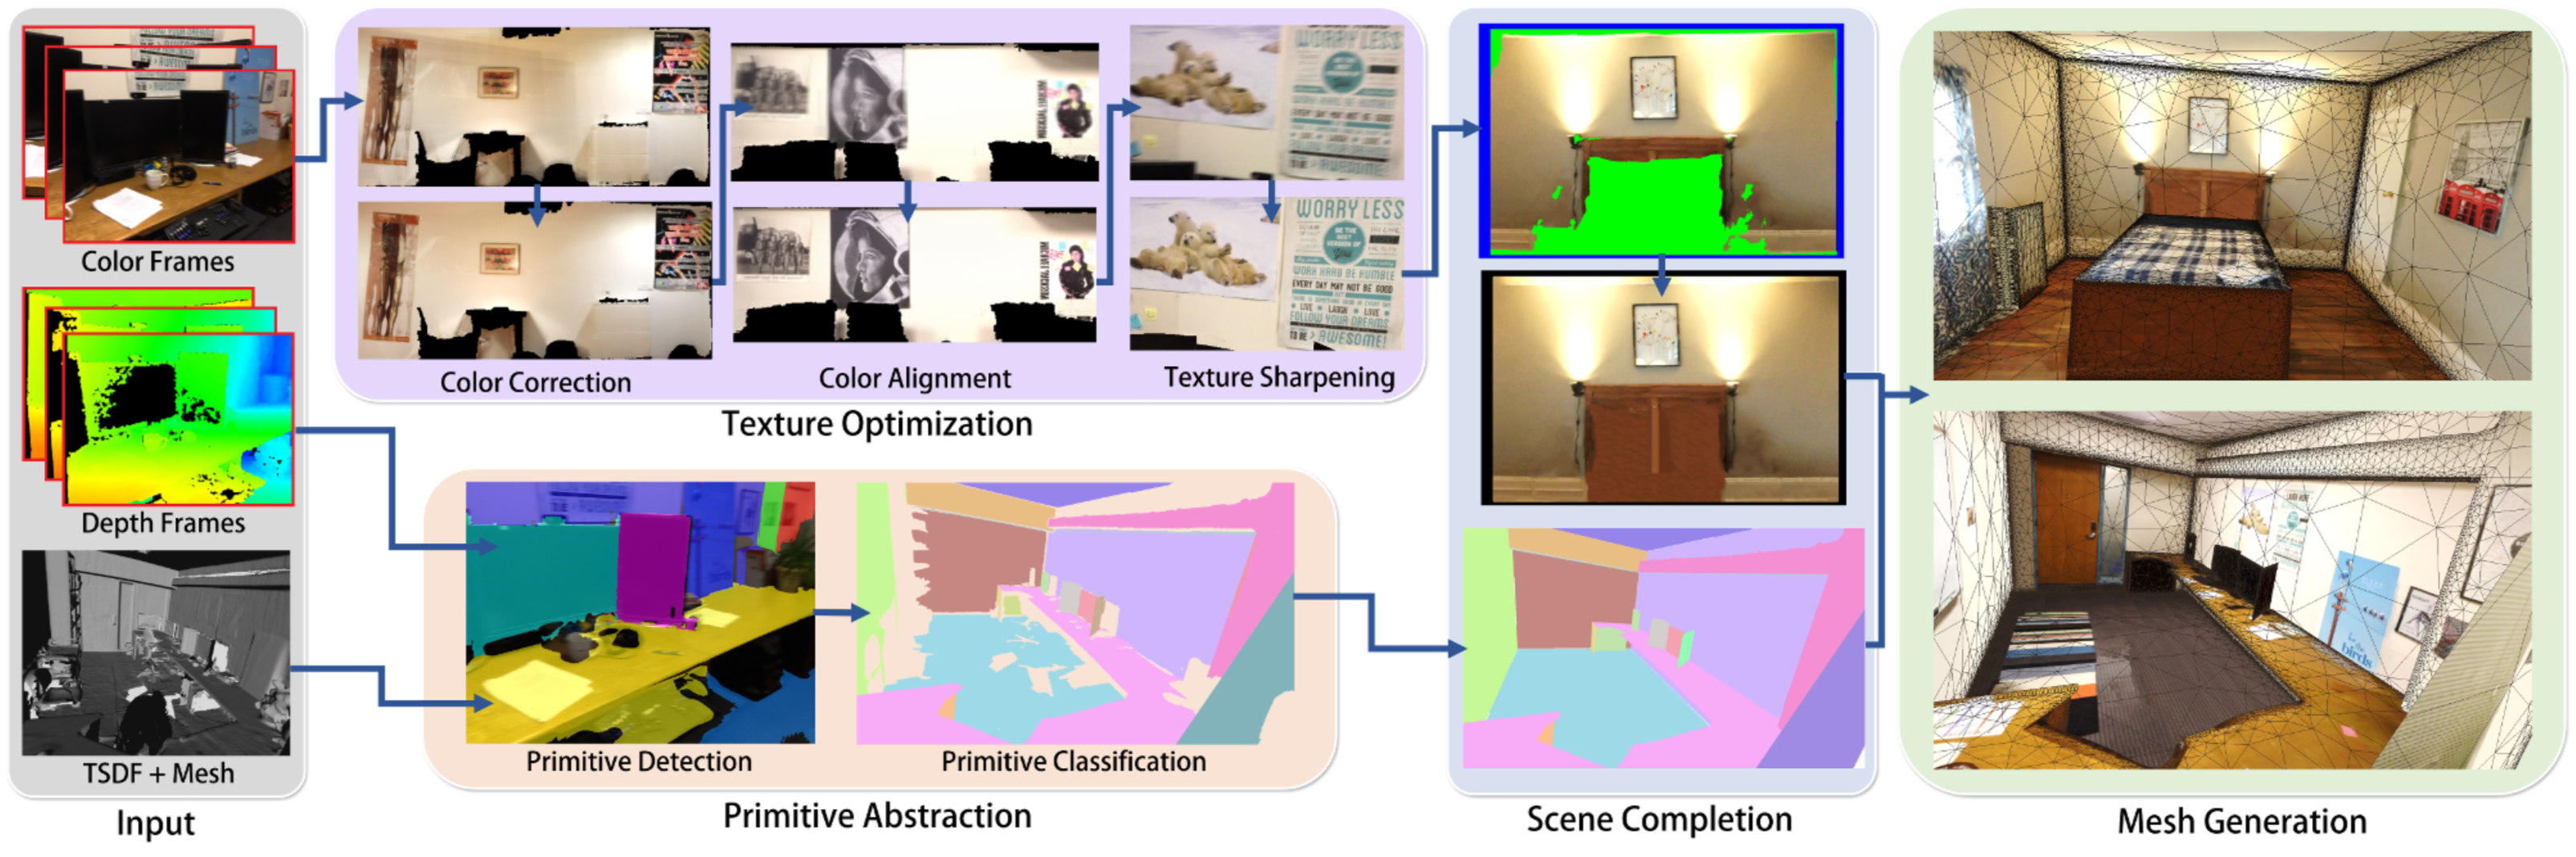
\includegraphics[width=\textwidth]{3dlite/fig2.png}
	\caption{Framework overview: our method takes a set of RGB-D frames as input, from which we compute a primitive abstraction that is used to optimize for sharp surface textures and infer missing scene parts. In the end, we obtain a low-polygonal, lightweight 3D reconstruction.
	}
%	\vspace{-0.2cm}	
	\label{fig:3dlite-overview}
\end{figure}
From an input RGB-D video, 3DLite\footnote{This section is mainly based on our work~\cite{huang20173dlite}.} first computes a primitive-based abstraction of the scene, and then leverages this representation to optimize for high-quality texture maps, as well as complete holes in the scene with both geometry and color; see Fig.~\ref{fig:3dlite-overview}.
We capture the input RGB-D stream with a handheld, consumer-grade RGB-D sensor.
Using a modern RGB-D reconstruction system (i.e., BundleFusion~\cite{dai2016bundlefusion}), we compute initial camera poses for each frame and a truncated signed distance field (TSDF) representation of the scene, from which we extract an initial mesh.
To generate the primitive-based abstraction, we detect planes for each frame, and then merge them into scene primitives according to the estimated camera poses (see section~\ref{sec:3dlite-plane-abstraction}).
We then optimize for the global geometric structure by favoring primitives to support a Manhattan world assumption, so as to encourage orthogonal and parallel structures.

From this lightweight representation of the scene, we then optimize for texture maps over the geometry, directly addressing the issues of motion blur and small camera pose misalignments.
We apply an exposure correction to achieve consistent color across the input images, which may vary with auto-exposure and white balancing (see section.~\ref{subsec:3dlite-color-transfer}).
We must then refine the camera poses to precisely align the color frames to the new model geometry.
To this end, we build upon the approach of Zhou and Koltun~\cite{zhou2014color} to optimize for refined camera poses and non-rigid image corrections.
For our large-scale scanning scenario, we introduce sparse color feature and geometric primitive constraints to help bring the optimization into the basin of convergence of a dense photometric consistency energy (see section~\ref{subsec:3dlite-color-align}).
In order to account for motion blur in input color images, we introduce a method to sharpen color projected from input frames to the model.
Rather than select sharpest keyframes throughout the input video, which may still select relatively blurry frames or lose color information by filtering out too many frames, we seek sharp image regions, from which we formulate a graph-cut based optimization for image sharpness and coherence (see section~\ref{subsec:3dlite-color-sharp}). 
%\angie{plz check this sharpening part} \jingweiNote{Additionally, we select $\triangle I$ from sharpest region, and optimize the final texture combining $\triangle I$ and averaged color. Do we describe it here?}
This leads to a high-quality texture map over the known geometry.

We then complete the textured model to fill holes that were occluded or unseen in the original scan.
While general, high-resolution scene completion is a very challenging task, our primitive-based abstraction enables effective hole-filling for both geometry and color on our scene representation.
To complete the geometry of the model, we extrapolate primitives in unobserved space according to the camera trajectory, such that each primitive meets either another primitive or empty space (see section~\ref{subsec:3dlite-extrapolate}). %\angie{is this actually true? also are we doing things different from dzitsiuk2016noising?} \jingweiNote{We extrapolate two planes to connect them, otherwise we don't extrapolate any plane even if there is unobserved space. Should be similar to dzitsiuk2016noising, but they really don't have a good explanation on this part.}
We then complete the color in these regions through image inpainting, following  Image Melding~\cite{darabi2012image} (see section~\ref{subsec:3dlite-inpaint}).
This produces a clean, complete, lightweight model mapped with sharp textures.
\section{Primitive-Based Abstraction}
\label{sec:3dlite-plane-abstraction}

To compute our primitive-based abstraction of a scanned scene, we first detect planes for each input frame, then merge these detected planes into a globally consistent set of primitives, and finally perform a structural refinement, optimizing under parallel and orthogonal constraints.

\subsection{Frame-based Plane Detection}
\label{subsec:3dlite-plane-detect}

From an input RGB-D video sequence comprised of a set of depth and color frames $\{f_i = (\mathcal{C}_i, \mathcal{D}_i)\}$, we first use a state-of-the-art RGB-D reconstruction system to obtain initial camera poses $T_i$ (frame-to-world) for each frame, and an initial surface $\mathcal{S}_0$.
For each frame, we detect planes using the fast plane extraction of Feng et al.~\cite{feng2014fast}. 
Instead of detecting planes directly on the input sensor depth, which is noisy and often contains holes, we operate on depth rendered from $\mathcal{S}_0$.
This rendered depth contains data accumulated over previous frames, which regularizes out noise and incorporates more information than a single input depth map, and is also well-aligned to the model geometry $\mathcal{S}_0$.
For each detected plane $\mathcal{P}_k$ in frame $f_i$, we additionally store two terms containing information used for primitive merging and structural refinement, as described in Secs.~\ref{subsec:3dlite-plane-classify} and Sec.~\ref{subsec:3dlite-color-align}.
\begin{itemize}
    \item Plane parameter: $p=(n_x,n_y,n_z,w)$ where $\mathbf{n} = (n_x,n_y,n_z)$ is the unit normal. It represents the plane $\mathbf{n}\cdot \mathbf{x} + w=0$ in the camera space of $f_i$. 
    \item Distance Matrix: $\mathbf{D} = \frac{1}{N}\sum_{q} x_qx_q^T$, where $x_q$ is the world space position of the $q$-th pixel in the depth map. 
    We can then easily compute the average of square point-plane distances (ASD) of $\mathcal{P}_k$ with another plane $\mathcal{P}_l$ in frame $f_j$ as $(p_l^jT_j^{-1})\cdot \mathbf{D}\cdot (p_l^jT_j^{-1})^T$. 
\end{itemize}

\subsection{Primitive Classification}
\label{subsec:3dlite-plane-classify}

We need to aggregate the per-frame planar regions into a set of plane primitives representing the planes in the 3D scene.
Two planar regions $\mathcal{P}_k$ from frame $f_i$ and $\mathcal{P}_l$ from frame $f_j$ are determined to be the same primitive if they are close and have enough overlap. 
We consider $\mathcal{P}_k$ and $\mathcal{P}_l$ to be close if $\max(\textrm{ASD}_{k\rightarrow l}, \textrm{ASD}_{l\rightarrow k}) < \tau_c$ (in practice, we use $\tau_c = 0.05$m).
Overlap is computed by transforming $\mathcal{P}_k$ and into the camera space of $f_j$ and computing the percentage of overlapping pixels relative to the minimum number of pixels belonging to $\mathcal{P}_k$ and $\mathcal{P}_l$.
If this overlap percentage is greater than $\tau_o$ (we use $\tau_o = 0.3$), the regions are considered to overlap.

We perform this merging step hierarchically.
For key frames at interval $n = 10$ frames, we merge planes within each key frames' set of $n$ frames, and then merge planes among all key frames.
Each frame then contains a set of plane primitives labeled according to the resulting merged set.
By projecting the merged primitive labels from the frames onto $\mathcal{S}_0$, we obtain a primitive decomposition of the scene. 
Note that regions with multiple different primitive label assignments (typically occurring near intersections of different primitive) are removed from the primitive set.
Fig.~\ref{fig:3dlite-plane-classify} shows an example primitive decomposition of an office scan, with different primitive denoted by different colors, and gray denoting no label assignment.
 
\begin{figure}
    \centering
    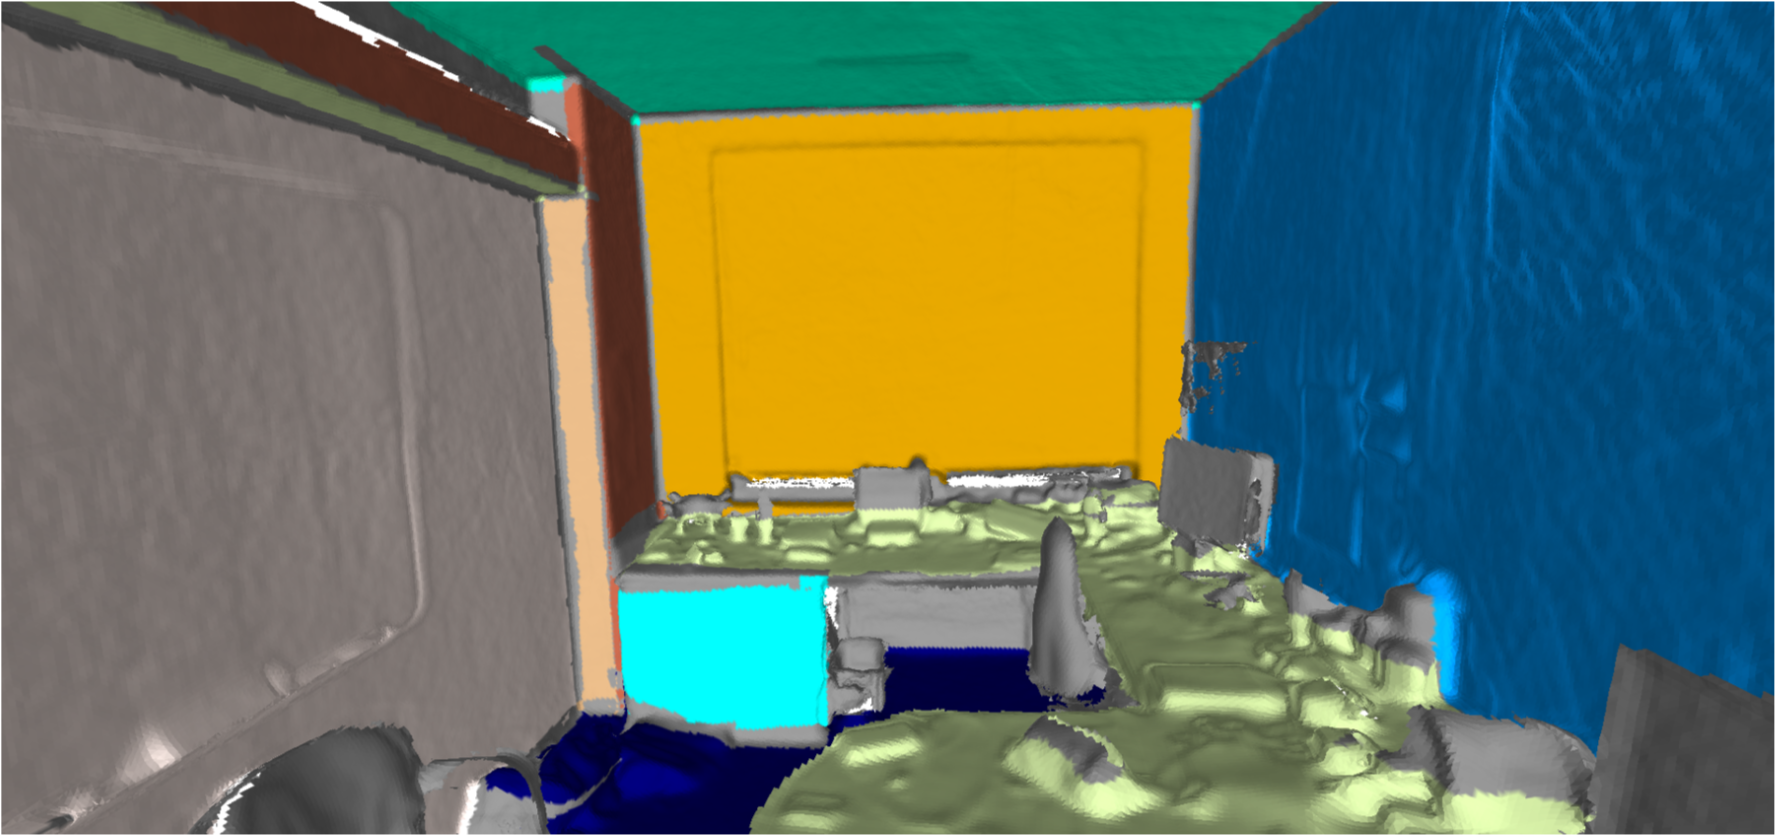
\includegraphics[width=0.97\linewidth]{3dlite/fig3.png}
    \caption{
    	Primitive decomposition: each plane primitive is denoted with a different color. Gray indicates no primitive association.
    }
    \label{fig:3dlite-plane-classify}

\end{figure}

To filter out any potential outliers from the primitive classification projection onto $\mathcal{S}_0$, we filter out small plane primitives (area less than $0.2$m$^2$) and use a RANSAC approach to filter out outlier points of larger primitives.
For a plane primitive $\mathcal{P}_k$, we check for outliers by randomly selecting $3$ of its associated vertices in $\mathcal{S}_0$ and fitting a plane $\mathcal{P}_k'$ to these vertices. 
A point is then considered an inlier for $\mathcal{P}_k'$ if its distance is smaller than $\tau_i$. 
Since $\mathcal{S}_0$ often contains warping in large plane primitives due to sensor noise and distortion, as well as camera pose micro-drift, we conservatively set $\tau_i = 0.1$m.
We repeat this process for $128$ iterations, and update $\mathcal{P}_k$ with the best fitting plane to the largest set of inliers in the least squares sense.

\subsubsection{Structural Refinement}
\label{sec:fit-refine}

Since we use a relatively conservative inlier threshold to compute the plane primitives, planes which should be orthogonal or parallel to each other are typically off by a few degrees.
We thus perform a structure refinement optimization on the planar primitives to encourage them to conform to a Manhattan world.
Similar to Halber and Funkhouser~\cite{halber2016fine}, we formulate an energy minimization using parallel and orthogonal constraints:

\begin{align}
	E_s &= E_d + \lambda E_a\, \\
    E_d &= \sum_{i}^{\#\textrm{planes}} \sum_{j}^{\#\textrm{plane verts}} D(\mathcal{P}_i,v_{ij})^2\,,\\
    E_a &= \sum_{i,j\in \Omega} |A(\mathcal{P}_i,\mathcal{P}_j)-90\cdot n_{ij}|^2\,.
\end{align}

For each plane primitive $\mathcal{P}$, $E_d$ measures the plane fitting error, where $D(\mathcal{P},v_i)$ is the distance from an inlier vertex $v_i$ to $\mathcal{P}$. 
$E_a$ measures the angle error between orthogonal planes, where $A(\mathcal{P}_i,\mathcal{P}_j)$ is the angle of two planes, $\Omega$ is a set of parallel and orthogonal plane pairs. 
The set $\Omega$ is collected by testing each pair of plane primitives, and adding them to the set if the angular difference between their normals lies in $[90n_{ij}-10, 90n_{ij}+10]$, where $n_{ij}\in \{0,1,2,3\}$. 
The final energy $E_s$ is then a linear combination of $E_d$ and $E_a$, with $\lambda=\frac{E_a^0}{E_d^0}$ to balance the plane fitting error and structure error.

The optimization typically converges in about $10$ iterations, with resulting angle errors less than $1^{\circ}$ and plane fitting error about $1.1$ times larger. 
%The angle error of each pair of planes in $\Omega$ is smaller than $1^{\circ}$, while the plane fitting error is about 1.1x bigger. 
As a result, we can rectify the orthogonal structure of the planar primitives with very small trade-off from fitting accuracy.
From this optimized result, we can produce a lightweight, clean mesh $\mathcal{S}_p$ by projecting the vertices of $\mathcal{S}_0$ to their associated primitives, as shown in Fig~\ref{fig:3dlite-plane-fit}(a). 

\subsection{Texture Optimization}
\label{sec:approach-texture}

We aim to map our primitive-abstracted geometric model $\mathcal{S}_p$ with sharp, clear textures to produce a visually compelling 3D model.
It is not suitable to directly project pixels from each color frame to the geometric model, due to the issues of motion blur and camera misalignments.
In our texture optimization step, we directly address these problems with a texture optimization method to solve for refined camera poses and image warping, as well as a texture sharpening step which considers per-pixel image sharpness to solve for globally crisp colors.

\subsubsection{Color-based Primitive Refinement}
\label{subsec:color-plane-refine}
\begin{figure}
    \centering
    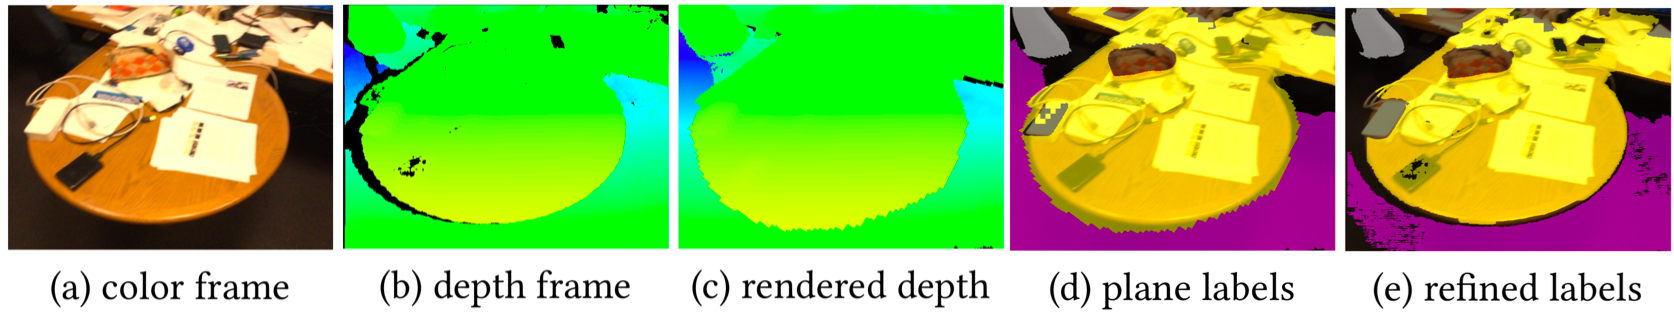
\includegraphics[width=\linewidth]{3dlite/fig4.png}
    \caption{Color-based primitive refinement: (a) Input color. (b) Input depth. (c) Rendered depth. (d) Primitive classification from rendered depth. (e) Refined primitive classification according to the color frame.}
    \label{fig:3dlite-color-boundary-refine}
\end{figure}
Since we originally detected plane primitives from rendered depth (Sec.~\ref{subsec:3dlite-plane-detect}), there may be some disagreement along primitive boundaries with the input RGB-D frame.
Thus pixels that are close to primitive boundaries are easily mis-classified, and we must re-classify them to agree with the input color images. 
To ensure that primitive labels are coherent in the image domain and maintain boundaries consistent with the input color frames, we formulate a graph-cut~\cite{boykov2001fast} based energy minimization problem:
\begin{equation}
E_l = \sum_p D(p, l_p) + \sum_{p,q} V_{pq}\delta(l_p,l_q)\,.
\label{eq:color-boundary-refine}
\end{equation}

Here $D(p,l_p)$ indicates the penalty for pixel $p$ to be classified as $l_p$. 
For confident regions, we won't change their labels $l_p^0$. 
So $D(p,l_p)$ is $1$ for $l_p=l_p^0$ and $\inf$ for other labels. 
For regions that need to be reclassified, $D(p,l_p)=1$ for all labels $l_p$. 
We additionally have a penalty at the boundary of the primitives, $\delta(l_p,l_q)$: $p$ and $q$ are neighbor pixels and $\delta$ is 1 if $l_p\neq l_q$ and 0 otherwise. 
$V_{pq}$ measures how good it is to cut between $p$ and $q$, depending on their color differences. We set
$V_{pq}=e^{\left(||\mathcal{C}(p)-\mathcal{C}(q)||^2\right)/\sigma^2}$.  %$V_{pq}=e^{\frac{||\mathcal{C}(p)-\mathcal{C}(q)||^2}{\sigma^2}}$. 
For our experiments, we re-classify pixels within $10$ pixels of the boundary of a $640\times 480$ image, and use $\sigma=30$ with colors $\mathcal{C}(x)\in[0,255]$.
Figure~\ref{fig:3dlite-color-boundary-refine} shows the result of our refinement.

\subsubsection{Color Transfer Optimization}
\label{subsec:3dlite-color-transfer}
In solving for a texture mapping, it is important to ensure consistent color across different views (e.g., due to auto-white balancing or auto-exposure).
This can be achieved by transferring colors with a mapping function.
For example, NRDC~\cite{hacohen2011non} search for correspondences between images, and optimizes for such a mapping function to transfer color style from one image to another.
In the scenario of RGBD scanning, correspondences can be easily acquired from camera poses and geometry. 
Zhang et al.~\cite{zhang2016emptying} solves the problem by minimizing vertex radiance error viewed from different color frames, given the exposure. 
In order to model white balance and exposure changes, we refer to the NRDC model to transfer colors using three spline curves ($B_j(r,g,b)=(B^1_j(r),B^2_j(g),B^3_j(b))$) for the rgb channels of the $j$-th frame. 
Then for a 3D point $p_i$ and it's corresponding pixels $\{q_{ij}\}$ in frames $\{j\}$ under the current camera poses, we want the color $C(p_i)$ to be close to $B_j(q_{ij})$:
\begin{equation}
E_t = \sum_{i} \sum_{j} ||C(p_i) - B_j(q_{ij})||^2 + \lambda \sum_{i} \sum_{j} (B_j'(x_i)-1)^2\,.
\end{equation}
While \cite{zhang2016emptying} use the first frame as a reference exposure, we don't need this constraint. 
Instead, we regularize the derivatives of the transfer functions $B'_j(x_i)$ to be $\approx 1$. 
This helps preserve the variance of the color. 
We use $\lambda = 0.1$, and $x_i$ is a sequence of 10 integers from 0 to 250 with interval 25.
Since this optimization depends on the quality of the camera transforms, we iterate this color correction step with the color image alignment optimization described below.

\subsubsection{Refined Texture Map Alignment}
\label{subsec:3dlite-color-align}
Key to achieving high-quality texture is obtaining precisely aligned color frames.
This is a challenging task, as there are artifacts from consumer-grade sensors and the geometry is often imprecise.
The color map optimization approach of Zhou and Koltun~\cite{zhou2014color} considers fixed geometry and jointly optimizes for color camera poses and image warping parameters.
This reduces the dimensionality of the problem, using image warping to reduce potential color misalignment from geometric error, achieving compelling results for object scans.
However, their optimization relies on dense photometric error, which has a relatively small basin of convergence and is thus rather sensitive to initial pose estimates.
For our large-scale scanning scenario, this energy is not very robust to the variance in initial camera poses.

In our formulation, we solve for a set of camera parameters for each frame separately from non-rigid correction, which we found to be more effective in practice. 
We adopt the idea of EM optimization with the help of dense color errors from Zhou and Koltun, and solve to maximize photo-consistency.
To aid convergence, we additionally introduce sparse feature and primitive-based constraints into the optimization.
Thus our energy is defined as
$$ E(\mathbf{T})=E_c(\mathbf{T}) + \lambda_s E_s(\mathbf{T}) + \lambda_p E_p(\mathbf{T})\,, $$
where $E_c$ represents the dense photometric energy, $E_s$ the sparse feature term, and $E_p$ primitive relationship constraints, and we solve for rigid camera poses (camera-to-world) $\mathbf{T}=\{T_i\}$ for each frame.
Following Zhou and Koltun, we also optimize for proxy variables $C(p_i)$ denoting the color at 3D point $p_i$ on the geometry surface.
We perform this optimization hierarchically in coarse-to-fine fashion to aid convergence at fine-scale resolution, using 3 hierarchy levels in which $p_i$ are sampled at $0.032$m, $0.008$m, $0.002$m from the primitive-abstracted $\mathcal{S}_p$, respectively.
$\lambda_s$ and $\lambda_p$ are set such that $E_c(\mathbf{T}_0)=\lambda_s E_s(\mathbf{T}_0) = \lambda_p E_p(\mathbf{T}_0)$.

\paragraph*{Sparse Term.}
In our sparse matching term, we minimize the sum of world-space distances between pairs of sparse feature correspondences transformed from image space to the space of the 3D primitives. 
For a frame $f_i$ and plane primitive $\mathcal{P}_k$, we transform a pixel $p_i$ under the homography $H_k^i$, depending on $\mathcal{P}_k$ and the camera pose $T_i$, to bring it into the space of the primitive $\mathcal{P}_k$.
Then for a pixel correspondence $\{p_{im},p_{jm}\}$ from frames $f_i$ and $f_j$ and which correspond to 3D primitives $\mathcal{P}_k$ and $\mathcal{P}_l$ (when projected in 3D under the current camera poses), we optimize for the energy
% Suppose corresponding pixels $p_i$ and $p_j$ are from frames $f(p_i)$ and $f(p_j)$, their distance in the space of the plane will be $H(||\mathbf{T}_{f(p_i)}) p_i - H(\mathbf{T}_{f(p_j)}) p_j||$} \angie{should specify what i and j are in the energy} 
\begin{equation}
E_s(\mathbf{T}) = \sum_m^{\#\textrm{corr}} ||H_k^ip_{im} - H_l^j p_{jm}||^2\,.
\label{eq:pose-optim-sparse}
\end{equation}

Sparse features are detected by projecting each color frame into the plane primitives, detecting SIFT~\cite{lowe2004distinctive} features in the projected images.
Correspondences are determined by SIFT matching followed by a verification step to ascertain that there is a valid 2D rigid transform bringing one set of correspondences from an image to another.
Valid correspondence features are then back-projected to the original color frames to compose the sparse feature set. 
This produces a robust set of feature correspondences, since the projection into a 3D plane does not rely on depth maps which contain noise and distortion, and matching in the warped space contains reduced scale and affine variance than in the original color images.

\paragraph*{Primitive Constraint Term.}
We restrict the per-frame planar regions computed in Sec~\ref{subsec:3dlite-plane-detect} to align well with $\mathcal{S}_p$, geometrically.
\begin{equation}
E_g(\mathbf{T}) = \sum_{i} \sum_{j} (P_j T_j^{-1} p_i)^T (P_j T_j^{-1} p_i)\,.
\label{eq:pose-optim-geo}
\end{equation}
Here, $p_i$ is the homogeneous coordinate of the sampled 3D points from $\mathcal{S}_p$. $P_j$ is the camera-space plane parameter (as in Sec.~\ref{subsec:3dlite-plane-detect}) of the $i$-th planar region of frame $j$.

\paragraph*{Dense Term.} 
Finally, the dense term measures photo-metric error from the color frames projected onto $\mathcal{S}_p$.
\begin{equation}
E_c(\mathbf{T}) = \sum_{i} ||C(p_i) - \sum_j I_j(\pi(T_j^{-1}p_i))||^2\,,
\label{eq:pose-optim-color}
\end{equation} 
where $p_i$ is in the set of sampled 3D points of $\mathcal{S}_p$ and $\pi$ denotes the perspective projection.

We solve for $E(\mathbf{T})$ by solving for both the per-frame transforms $\mathbf{T}$ and the proxy variable colors on the geometry $C(p_i)$.
After an initial three iterations at the coarsest resolution, we are able to compute very reliable sets of correspondences for a color transfer correction (as described in Sec.~\ref{subsec:3dlite-color-transfer}); after the color correction, we further optimize for refined camera poses at the middle and high resolutions for five and two iterations respectively.

%\angie{is this the same as the color map optimization? if so we could just refer to that. otherwise what exactly are the differences?} \jingweiNote{they are exactly the same.}
After solving for the rigid camera poses, we additionally optimize for non-rigid image warping to reduce color misalignment due to possible geometric error, following Zhou and Koltun~\cite{zhou2014color}.
\begin{comment}
Similar to Zhou et al.~\cite{zhou2014color}, we solve for a warping function for each image, $\xi : \mathbb{R}^2\rightarrow \mathbb{R}^2$, which deforms a regular grid $\mathbf{X} = {X_{mn} = (mw,nh)}; m,n\in\mathbb{Z}$ of size $w\times h$ on the image domain.
$\xi(\mathbf{X})$ is then computed as a bilinear interpolation of $\xi(X_{mn})$ at the four nearest grid points.
We then minimize the energy:
\begin{align}
\begin{split}
E_w(\xi) &= \sum_{i} ||C(p_i) - \sum_j I_j(\xi(\pi\cdot T_j^{-1}p_i))||^2 \\
&+ \lambda (||\xi(X_{mn})+(w,0)^T-\xi(X_{m+1,n})||^2\\
& + ||\xi(X_{mn})+(0,h)^T-\xi(X_{m,n+1})||^2)\,,
\end{split}
\label{eq:color-optim-warp}
\end{align}
regularizing the warping by restricting the neighbor grid points' offset to be close to the original state. 
For our experiments, we use $\lambda = 0.3$.
Note that we do not include $E_s$ and $E_g$ in this optimization, as $E_g$ is not changed by local image warping and the sparse features of $E_s$ are already aligned, and dense color error will also restrict these alignments to be fixed. \angie{not sure what the second half of the sentence means, regarding dense and sparse errors} \jingweiNote{Maybe we can throw it out. I mean the warping optimization won't make the sparse feature misaligned, because dense color constraints is usually consistent with sparse feature constraints (maybe it is not always true, so we remove it?.)}
\end{comment}

\subsubsection{Texture Sharpening}
\label{subsec:3dlite-color-sharp}
Motion blur is a common problem when capturing handheld video using commodity RGB-D sensors.
Even with perfect alignment of camera frames, a blurry image can still significantly decrease the quality of the model color. 
Most existing scanning methods average colors from all corresponding frames, or update the color online with a weighted combination. 
In order to mitigate this issue, the color map optimization of Zhou and Koltun~\cite{zhou2014color} selects sharpest keyframes every 1 to 5 seconds, with sharpness of a frame evaluated using the method by Crete et al.~\cite{crete2007blur}. 
However, when we applied this to our scenario, not all blurry frames were filtered out, and if keyframes were selected with interval greater than 1 second, color information was lost in some regions. 
In fact, in the room-scale setting, this tends to preserve views where the camera is closer to the scene, as such images typically have more objects and thus higher color variance.
However, we wish to preserve cameras with closer views to the scene, which capture textures with more detail.
Thus we instead aim to only map the sharpest regions of the images onto the geometry; i.e., for each primitive in $\mathcal{S}_p$ we map the sharpest region of color from any single image.
To this end, we consider both image pixel sharpness and image region sharpness in order to select key frames at an intervals of [10,20] frames.
For image pixel sharpness, we use the metric of \cite{vu2012bf}, and for image region sharpness we consider both pixel sharpness and visual density, where visual density measures the quality of the view of a pixel (accounting for far distances and glancing angles), and is defined as
\begin{equation}
r_j(p_i) = \left((T_j^{-1}\pi^{-1}(p_i))\big|_z\right)^{-2} \cdot \cos(\mathbf{r}\cdot \mathbf{n})\,,
\label{eq:visual-res}
\end{equation}
where $p_i$ is a pixel of frame $j$, $\mathbf{r}$ is the ray from the camera to $p_i$, and $\mathbf{n}$ the camera-space normal at the 3D point corresponding to $p_i$.
The region sharpness for a pixel is then defined as $S^{\textrm{reg}}_j(p_i)=S^{\textrm{pix}}(p_i)\cdot r_j(p_i)$. 
Since we wish to avoid noise potentially introduced by sampling from many different frames for similar 3D locations, we formulate a graph-cut~\cite{boykov2001fast} based energy optimization which further incorporates frame coherence:
\begin{align}
\begin{split}
E&=\sum_{p} |S_{l(p)}(p) - S^{\textrm{max}}(p)| + \\
&\lambda \sum_{(p,q)}||\mathcal{C}_{l(p)}(\pi(T^{-1}_{l(p)}p)) - \mathcal{C}_{l(q)}(\pi(T^{-1}_{l(q)}q))||\cdot \delta(l_p,l_q)\,,
\end{split}
\label{eq:3dlite-sharp-graph-cut}
\end{align}
solving for frame index $l(p)$ for each point $p\in\mathcal{S}_p$.
The first term encourages sharpness, with $S^{\textrm{max}}(p)$ denoting the sharpest possible score for $p$.
The second term encourages coherence by penalizing neighboring points $p$ and $q$ if they are associated with different frames, with penalty proportional to the respective color difference in order to achieve a seamless graph cut.
\begin{figure}
\centering
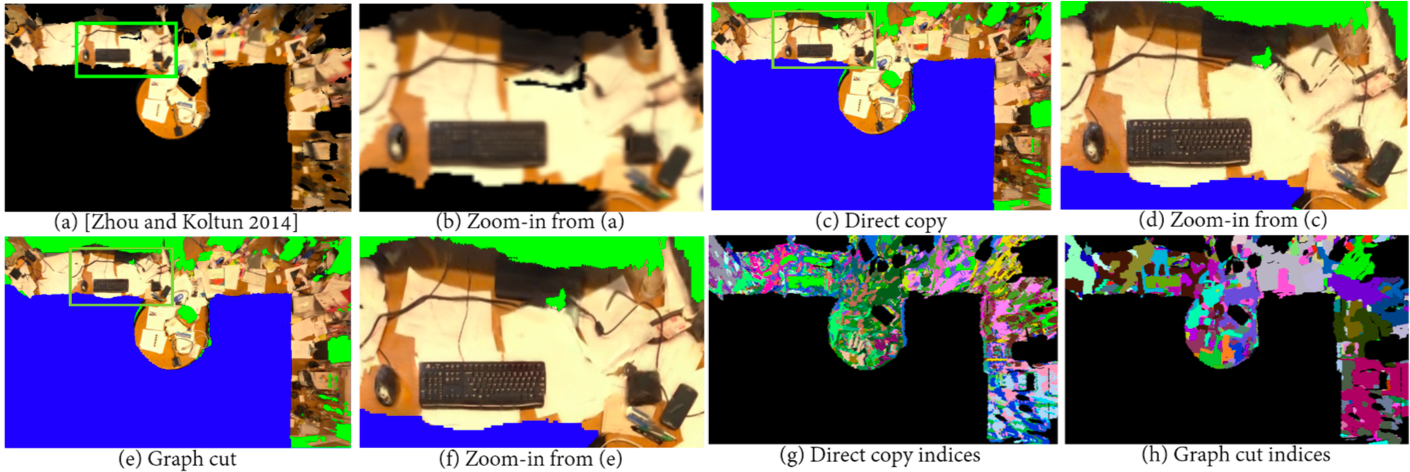
\includegraphics[width=\linewidth]{3dlite/fig5.png}
\caption{Texture generation from multiple frames: (a) Color map optimization~\cite{zhou2014color} (averaging). (b) Zoom-in from (a). (c) Direct copy from sharpest region. (d) Zoom-in from (c). (e) Balance sharpness and region coherence. (f) Zoom-in from (e). (g) Frame indices with sharpest local region. (h) Optimized frame indices for color sampling.
}
\label{fig:3dlite-sharp-graph-cut}
\end{figure}

Figure~\ref{fig:3dlite-sharp-graph-cut} shows a challenging example, where a table texture is composed of projections from the 147 sharpest color frames of more than 3000 images.
We see that directly sampling from frames with the highest region sharpness value ((c),(d)) improves upon the texture sharpness of Zhou and Koltun~\cite{zhou2014color} ((a),(b)), but contains some noise due to lack of coherence in the frames being sampled from. Our final texture sharpening result ((e), (f)) balances both sharpness and frame coherence, preserving sharpness while reducing noise.

Using direct color sampling can still result in noticeable artifacts when transitioning from sampling from one frame to another, as shown in Fig.~\ref{fig:3dlite-sharp-poisson}(b).
We perform a final step in to mitigate these effects in the sharpening process.
We combine the divergence map $\triangle C(p)$ from the labeling resulting from solving Eq.~\ref{eq:3dlite-sharp-graph-cut}, which represents texture information~\cite{perez2003poisson}, with the color map $\bar{C}(p)$ computed by averaging, and solve for the final texture $F(p)$ in the least squares optimization
\begin{equation}
E(F) = \sum_p ||F(p) - \bar{C}(p)||^2 + \lambda ||\triangle F(p) - \triangle C(p)||^2\,.
\label{eq:sharp-poisson}
\end{equation}
As shown in Fig.~\ref{fig:3dlite-sharp-poisson}, this maintains sharpness while removing boundary inconsistencies.

\begin{figure}
\centering
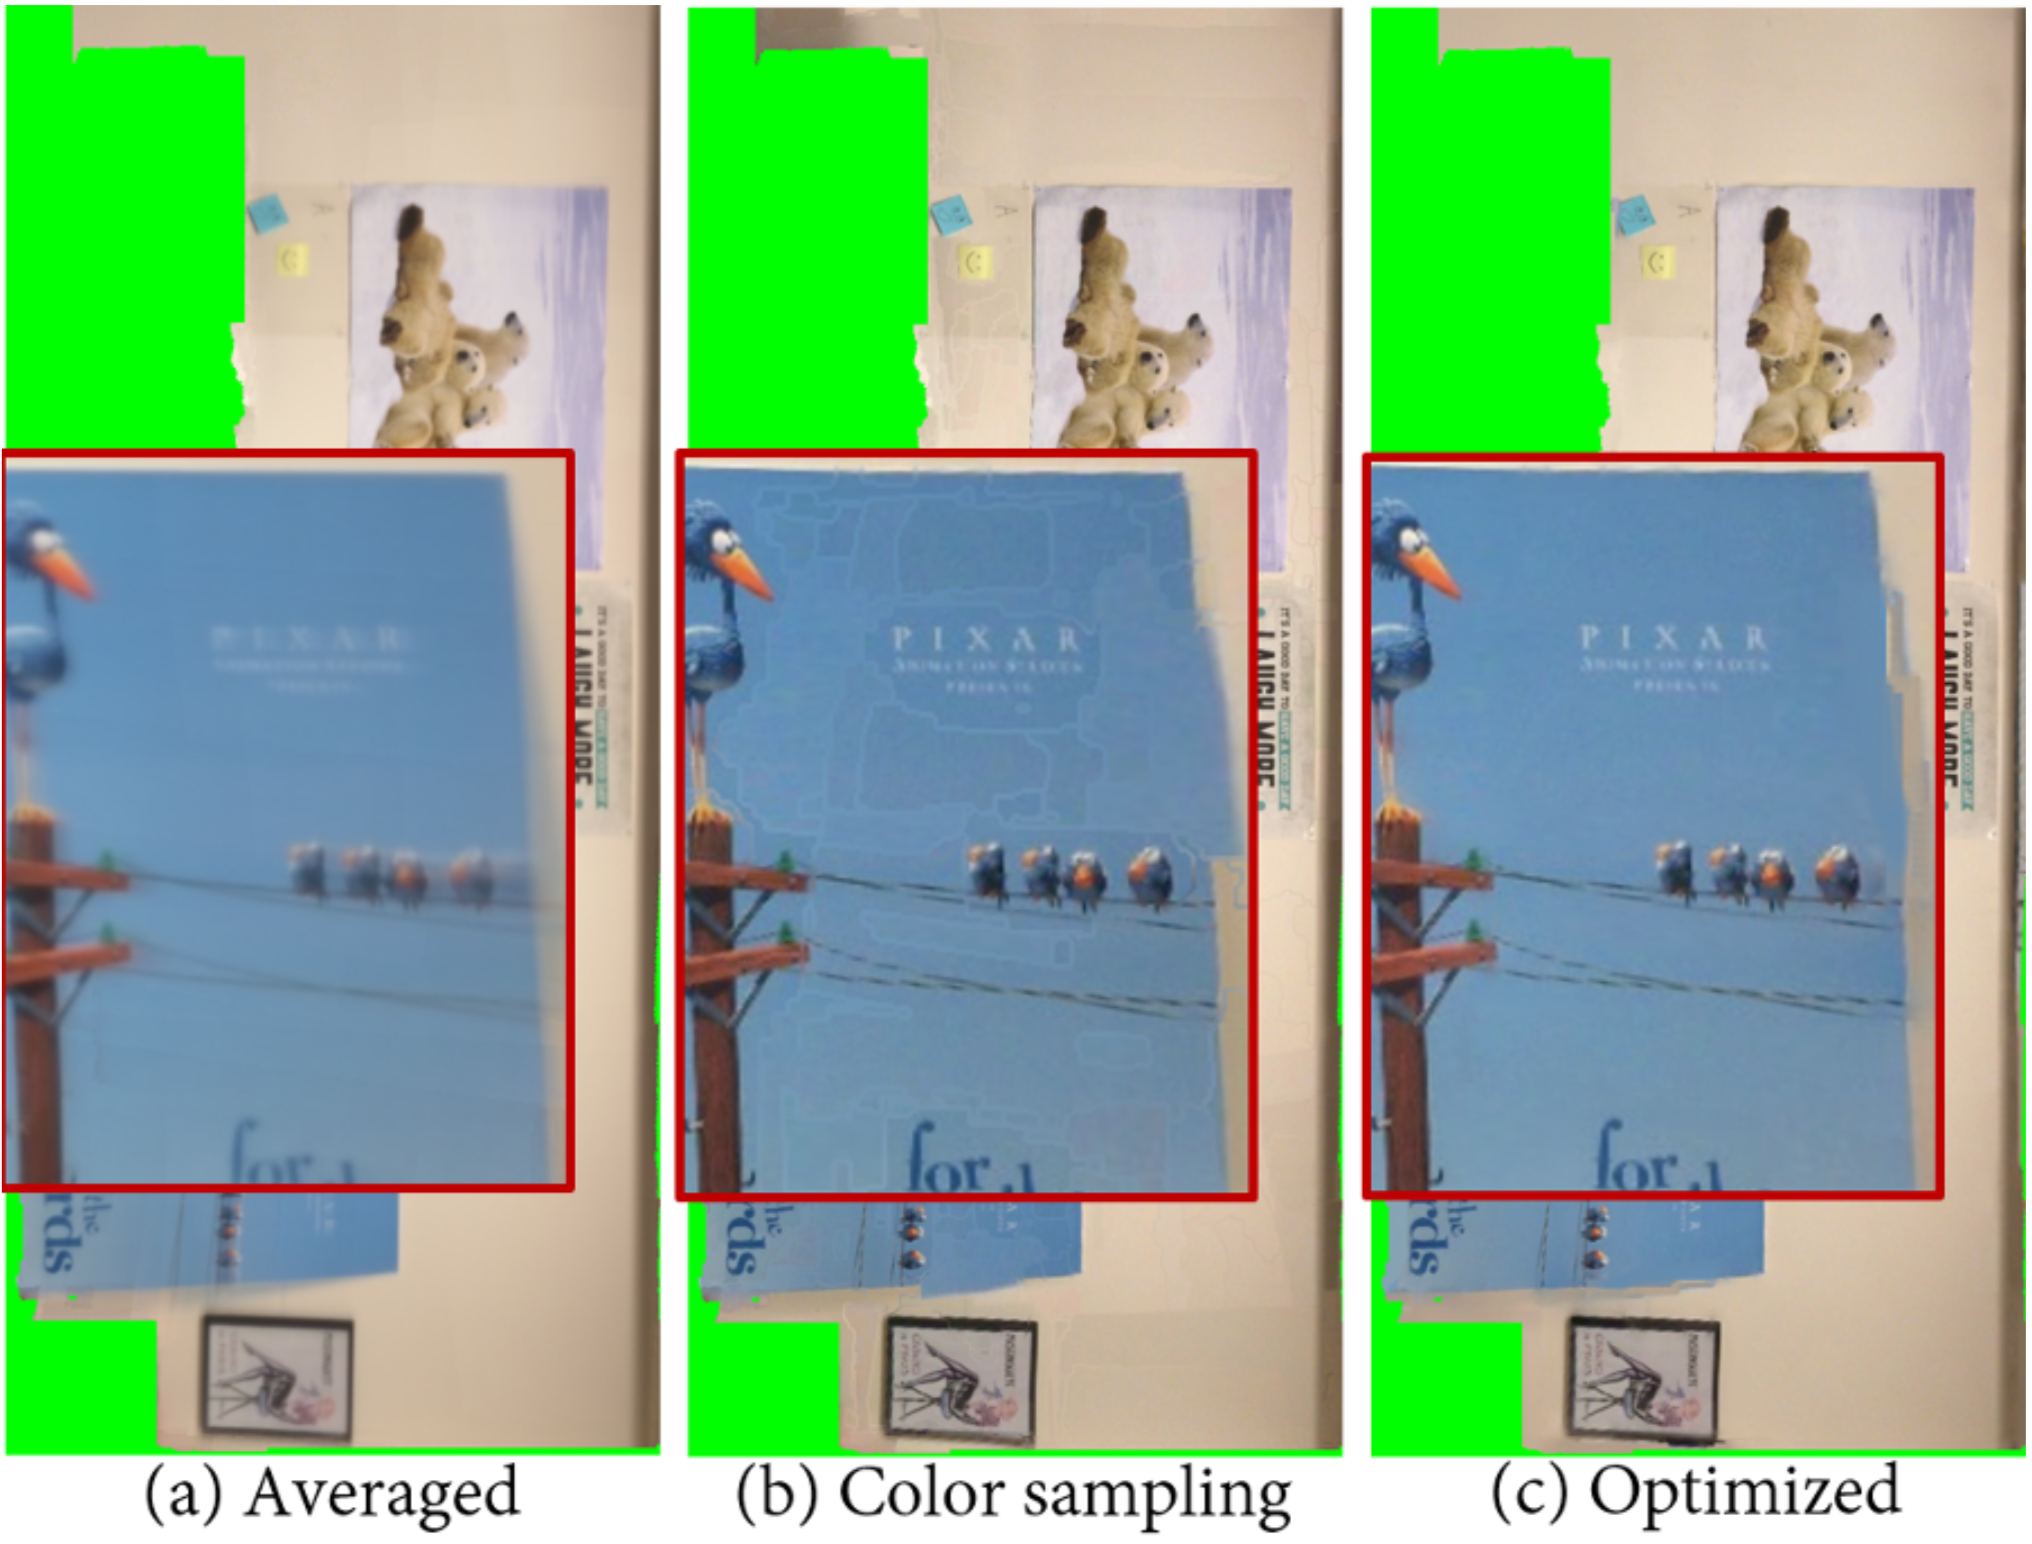
\includegraphics[width=0.8\linewidth]{3dlite/fig6.png}
\caption{Texture optimization combining averaged color and sampled divergence map. (a) Averaged color from all selected frames. (b) Direct color sampling from optimized frame indices. (c) Optimization combining averaged color and sampled divergence map.}
\label{fig:3dlite-sharp-poisson}
\end{figure}

\subsection{Scene completion}
\label{sec:completion}

While our texture-optimized, lightweight mesh contains sharp, compelling color, it nonetheless remains incomplete, due to occlusions or limited scanning coverage.
3D completion is a challenging task, as it typically requires example-based learning techniques~\cite{dai2017complete}, and the problem becomes cubically more complex with  higher resolutions and larger spatial extents.
We thus exploit our planar primitive abstraction to simplify 3D scene completion in both geometry and color.%, as it can be extrapolated to 
\begin{figure}
	\centering
    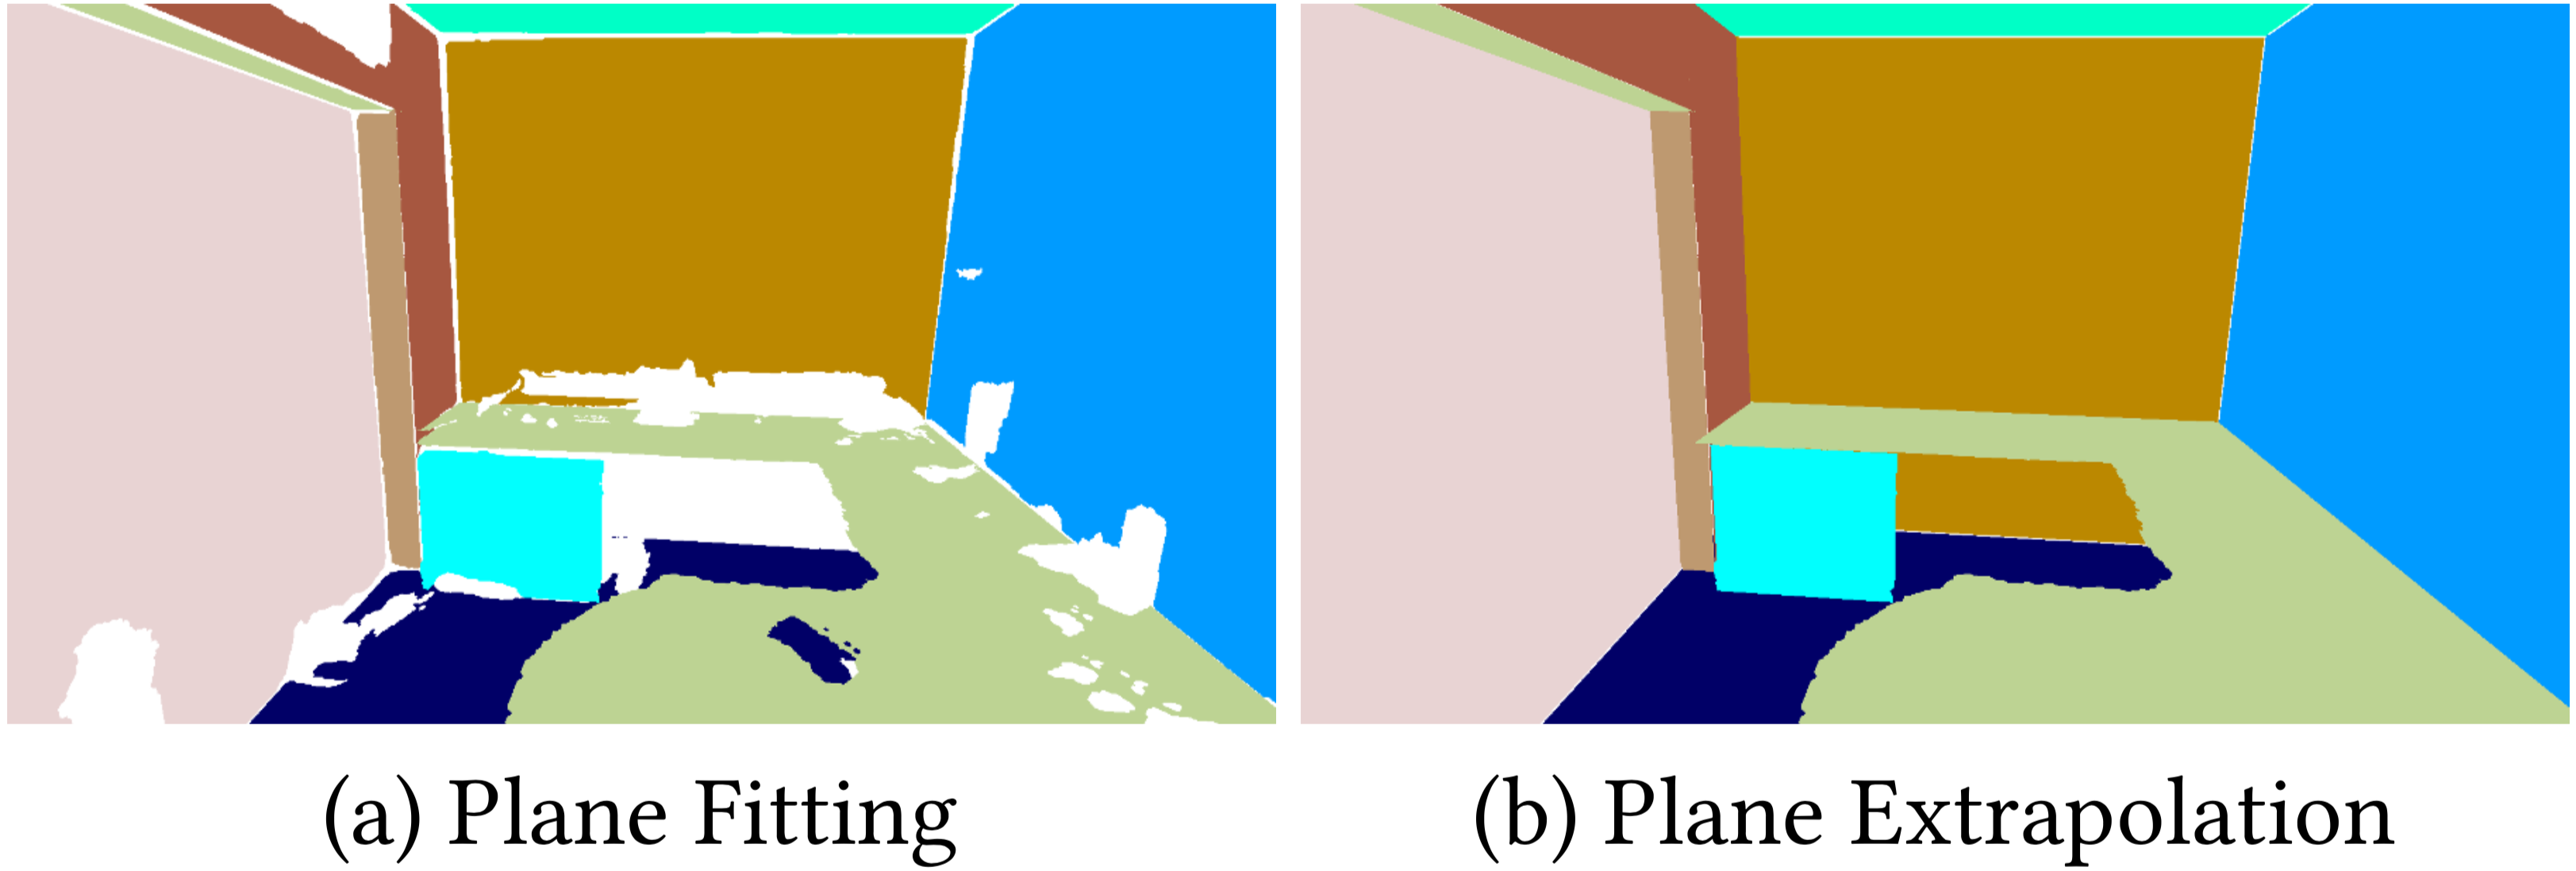
\includegraphics[width=0.8\linewidth]{3dlite/fig7.png}
	\caption{Primitive fitting and extrapolation: (a) After primitive fitting and structural refinement, we project vertices to the primitives, producing a clean mesh. (b) We extrapolate primitives in occluded regions to close the surface.}
	\label{fig:3dlite-plane-fit}
\end{figure}

\subsubsection{Geometry Completion}
\label{subsec:3dlite-extrapolate}
\begin{figure}
	\centering
	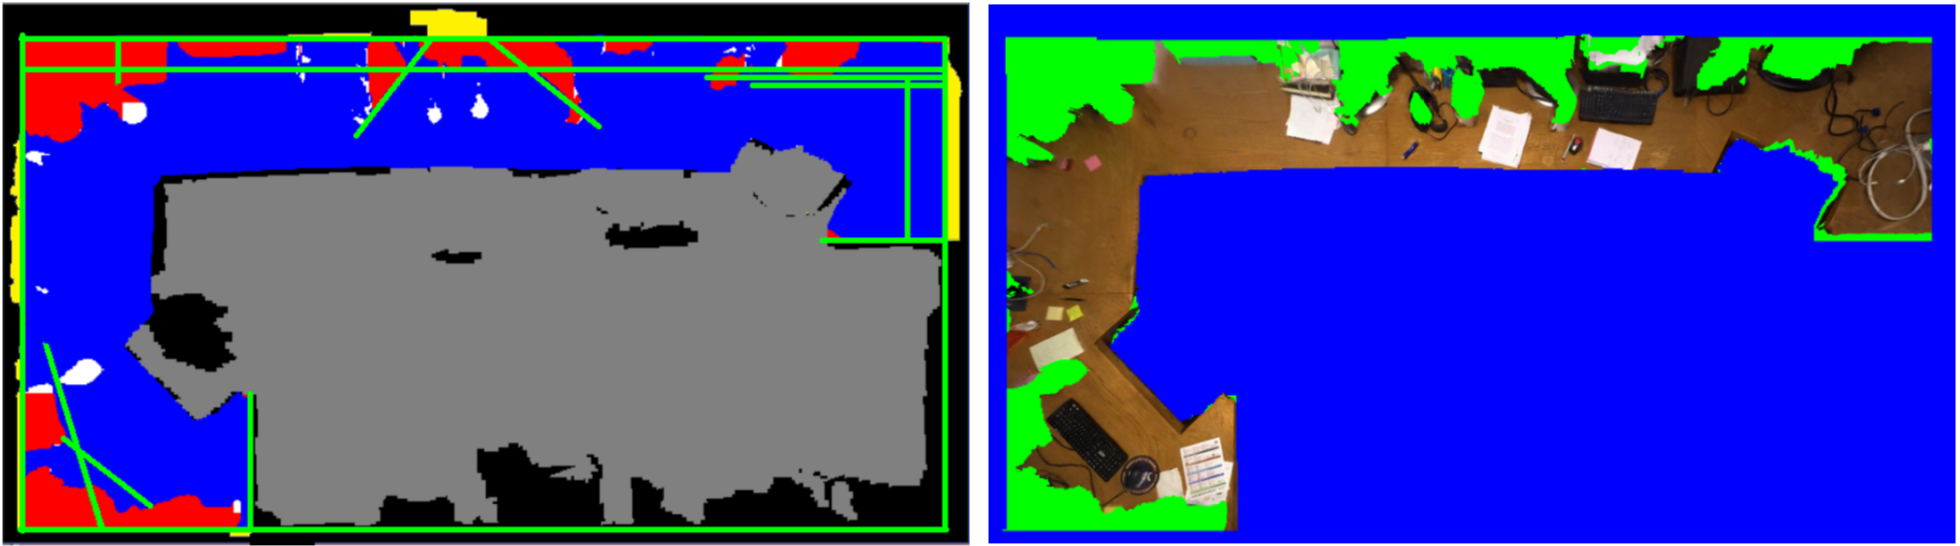
\includegraphics[width=0.8\linewidth]{3dlite/fig9.png}
	\caption{An example of extrapolation and hole filling. Left: Green lines represent possible intersections between sets of planes. Blue represents the original scene geometry, red the extrapolated regions, yellow removed original geometry extending past intersections, gray known empty space, and white self-contained holes which were filled. Right: Completed plane primitive with texture.}
	\label{fig:3dlite-plane-fill}
\end{figure}

A plane-based primitive abstraction enables geometry completion by plane extrapolation in unseen regions~\cite{dzitsiuk2016noising}.
We use several rules to guide our completion approach, visualized in Fig.~\ref{fig:3dlite-extrap-illus}:
\begin{itemize}
	\item Two planes should be extrapolated to their intersection if the extrapolated area is unobserved.
	\item If three planes will intersect each other, extrapolate them to meet at a corner if the extrapolated area is unobserved.
	\item No planes should be extrapolated into open space (observed to be empty). Note that we use the initial TSDF to determine known occupied, known empty, and unobserved space, according to the camera trajectory.
	\item Holes self-contained in a plane should be filled if they are in unobserved space.
\end{itemize}

We search for all pairs of planes satisfying the first rule and extrapolate them. 
Then, we find all triplets of planes under the second rule and extrapolate them. 
Our algorithm is invariant to the extrapolation order since the final state forces all planes to meet in unobserved areas.
For each pair of planar primitives, we attempt to detect potential extrapolation regions, and then repeat the same for all sets of three planar primitives which intersect. Finally, we fill in unobserved holes self-contained within planar primitives.
Note that while this process achieves successful completion for scenes in which parts of all major planes have been observed, we cannot generate geometry from scratch in the case of very large regions of unobserved scene geometry (see Sec~\ref{subsec:3dlite-limitations} for further discussion).

Figs.~\ref{fig:3dlite-plane-fit} and \ref{fig:3dlite-plane-fill} demonstrate our extrapolation and hole-filling to generate complete scenes.

\begin{figure}
	\centering
	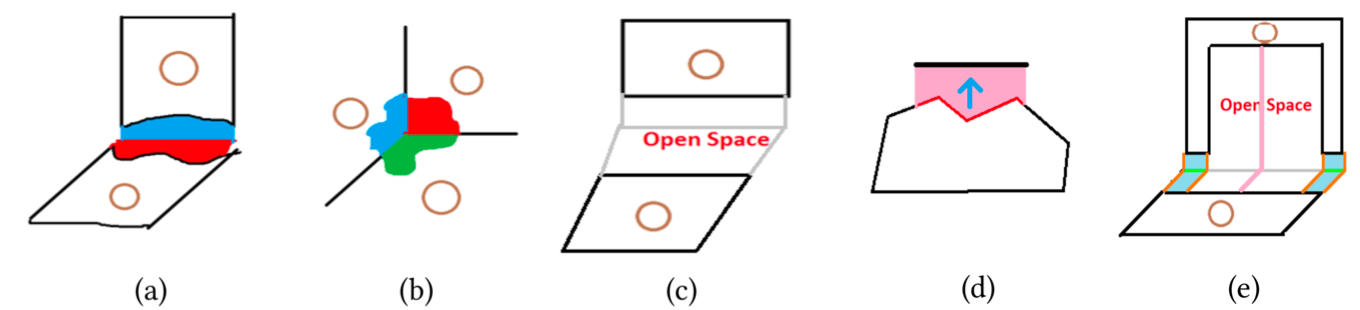
\includegraphics[width=0.8\linewidth]{3dlite/fig8.png}
	\caption{Rules for plane extrapolation. (a) Two planes should extrapolate to their intersection. (b) Three planes should extrapolate to their intersection. (c) No planes should be extrapolated through known empty space. (d) Extrapolation (light red) can be viewed as a certain boundary (red) extending in the direction (blue) orthogonal to the intersection line. (e) A more complex example, showing invalidation of potential extrapolation due to known empty space. Only the blue regions should be extended towards the intersection.}
	\label{fig:3dlite-extrap-illus}
\end{figure}

\subsection{Texture Completion}
\label{subsec:3dlite-inpaint}
Our plane-based primitive abstraction reduces the 3D texture completion problem into a two-dimensional one over plane textures.
As this texture synthesis problem is a classical one and has been well-studied~\cite{criminisi2004region,simakov2008summarizing,barnes2009patchmatch,darabi2012image,wang2016unsupervised,pathak2016context,yang2016high}, we employ state-of-the-art image inpainting techniques to complete texture in geometry-extrapolated regions.

Although recent deep learning based methods have shown impressive results, they require a large training set and are mostly constrained to fixed image resolutions. 
Thus we use Image Melding~\cite{darabi2012image}, a patch-based approach incorporating image transforms and gradients into a mixed $\ell_2/\ell_0$ optimization to achieve high-quality image inpainting.
We found the method to work well for most cases, except when there are incomplete regions of a texture which cover a distinct foreground and smooth background, or when there are shadows on the background, as shown in Fig.~\ref{fig:3dlite-synthesize}(b).
In these cases, we detect the background using image segmentation~\cite{felzenszwalb2004efficient}, and extend it to fill the entire image using laplacian smoothing (Fig.~\ref{fig:3dlite-synthesize}(c)).
We then combine the synthesized background with the foreground (Fig.~\ref{fig:3dlite-synthesize}(d)), and synthesize pixels less than $10$ pixels from the foreground using Image Melding (Fig.~\ref{fig:3dlite-synthesize}(e)).

\begin{figure}
	\centering
    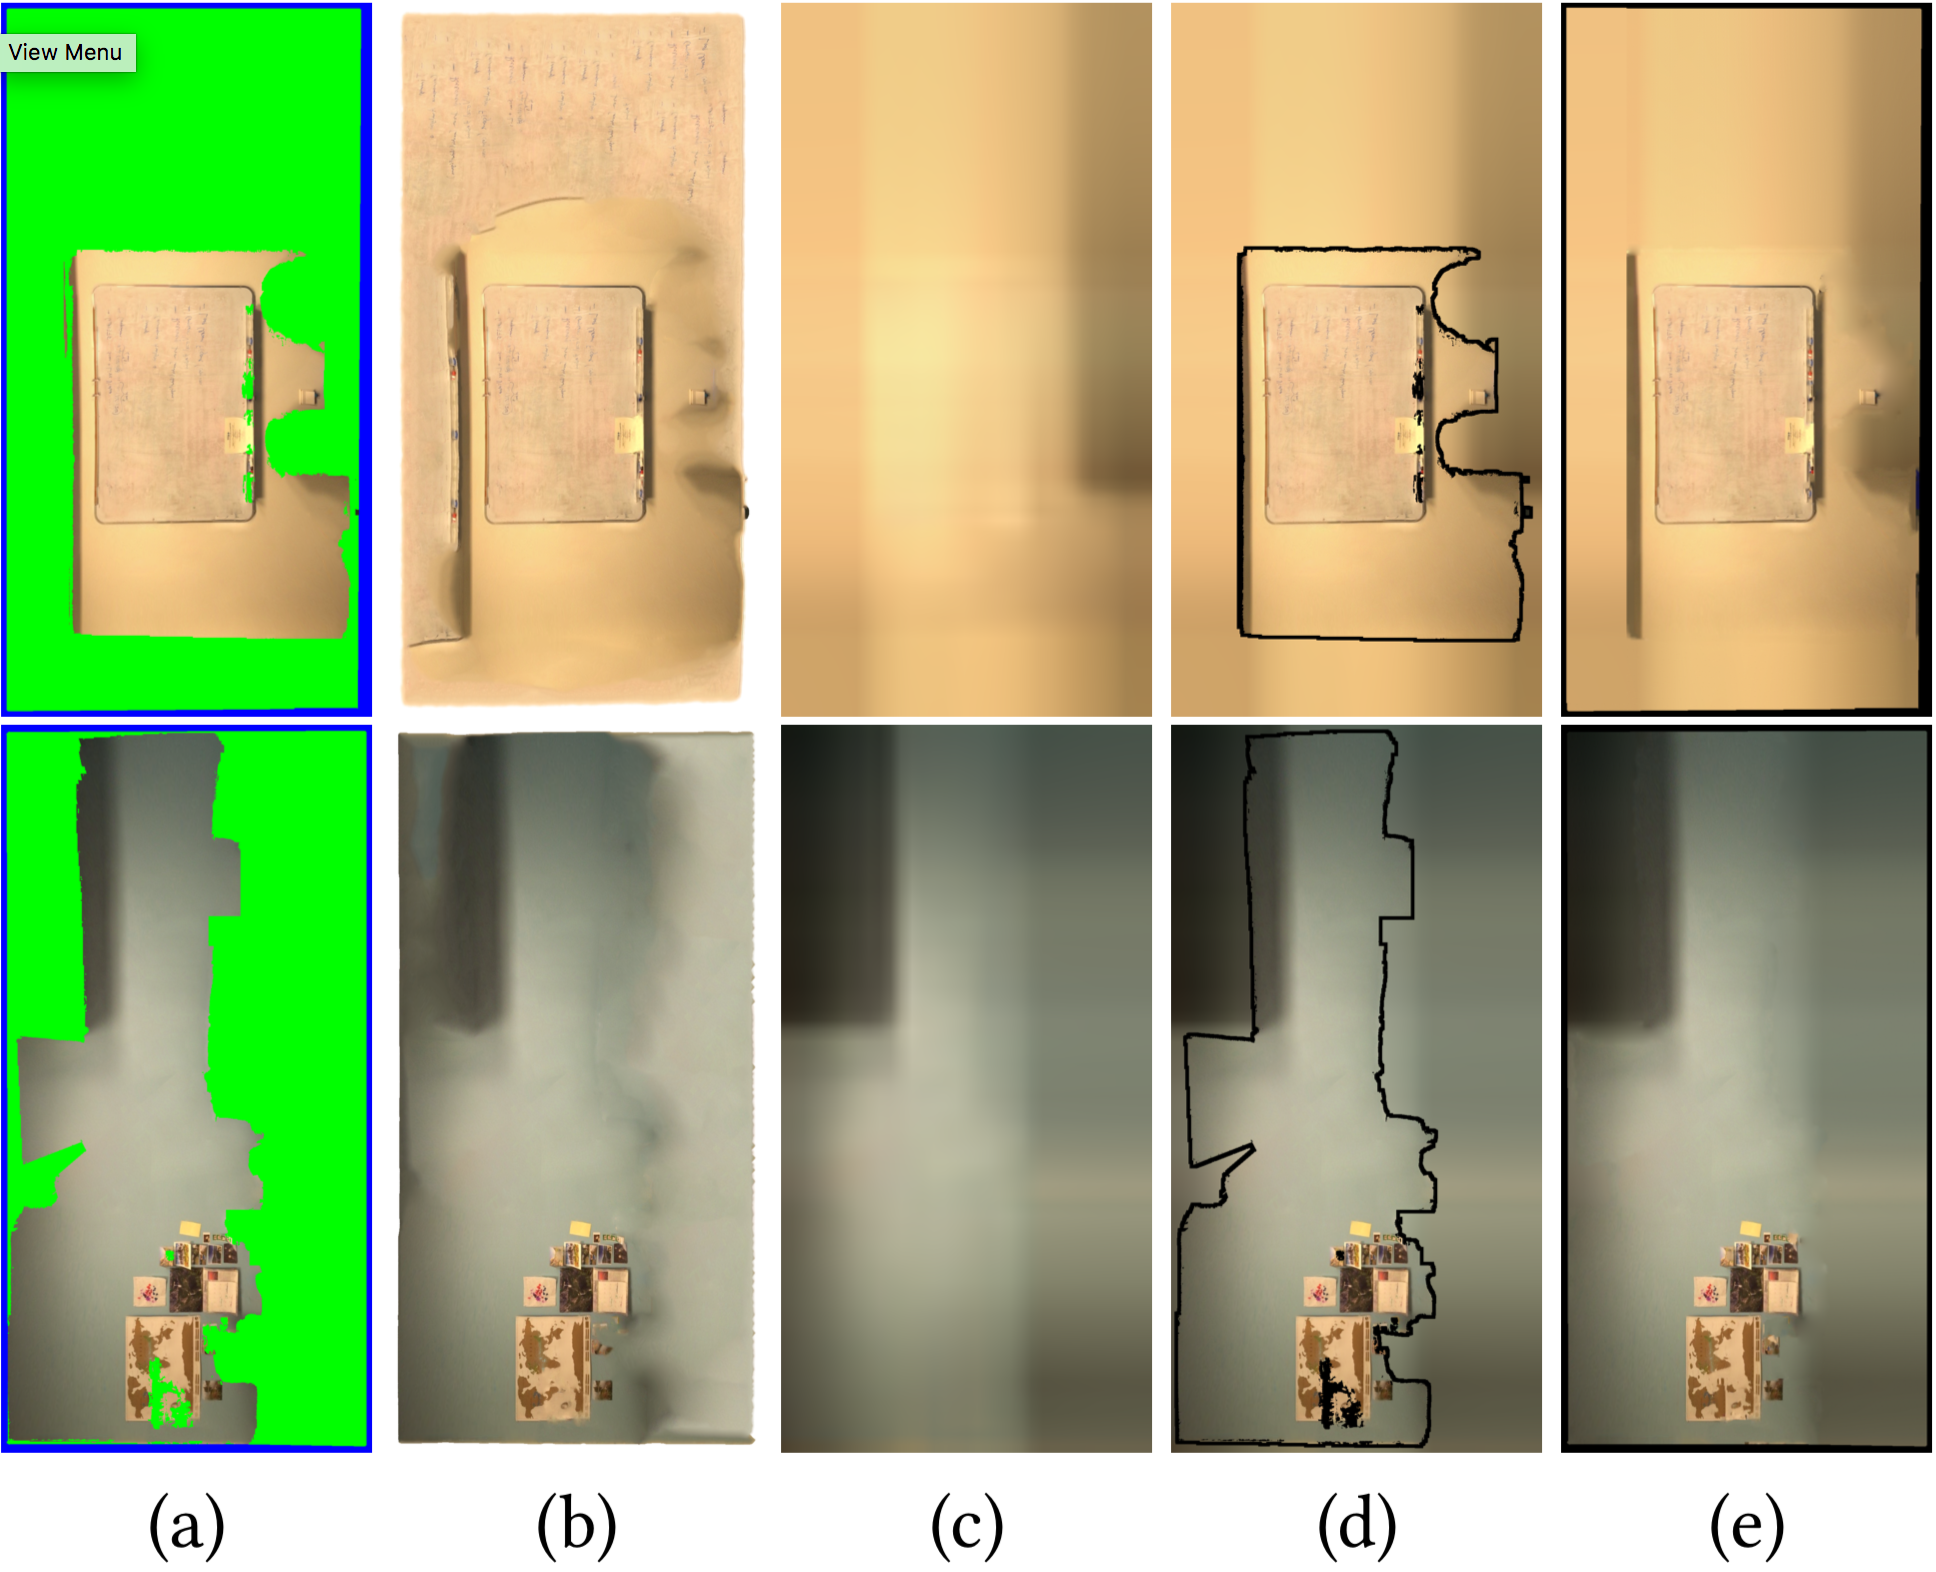
\includegraphics[width=0.8\linewidth]{3dlite/fig10.png}
	\caption{Texture completion. (a) Original texture with green denoting regions to be synthesized. (b) Direct application of Image Melding~\cite{darabi2012image}. (c) Background color estimation. (d) Combined background and original texture. (e) Remaining pixels inpainted with Image Melding.}
	\label{fig:3dlite-synthesize}
\end{figure}

\subsection{Mesh Generation}
\label{sec:approach-mesh}
In section, we discuss the procedure to generate the final light-weight mesh. 
We first denoise plane boundaries and then convert the planar primitive abstraction to a mesh, producing a final model $\approx 25$ times smaller than the original mesh.

\paragraph*{Boundary Refinement.}
Plane boundaries are often noisy, due to noise and distortion in the input sensor data and the initial reconstruction.
To denoise the boundaries, we smooth them with a combination of line and B-spline fitting.
Lines are fit to each vertex on the boundary (sampled at every 8mm) by using its $51$ neighboring vertices. 
A vertex belongs to a line if the condition number of the covariance of these vertices is larger than 50.
We then iteratively merge line-associated neighbor vertices together if their lines are no more than $5^\circ$ apart.
We fit B-splines to each consecutive sequence of vertices not belonging to any lines.

\begin{figure}
\centering
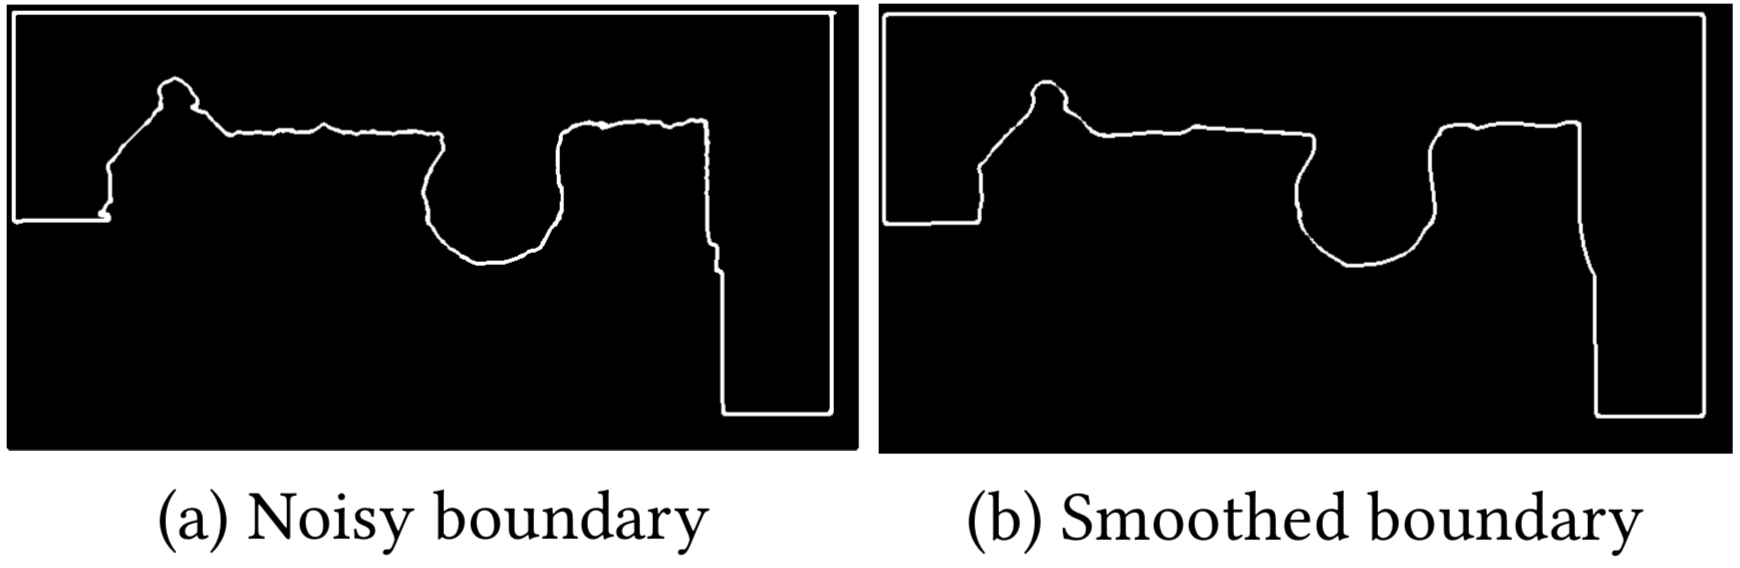
\includegraphics[width=0.8\linewidth]{3dlite/fig11.png}
\caption{Smoothing the boundary. Initial plane primitive boundaries are noisy (left), which we smooth with B-Splines and lines (right).}
\label{fig:boundary-fit}
\end{figure}

\paragraph*{Primitive Remeshing.}
To generate our final mesh, we triangulate the planar primitives using constrained Delaunay triangulation~\cite{chew1987constrained}. 
Figure~\ref{fig:3dlite-remesh}(a) shows the resulting simplified triangle mesh, which accurately preserves primitive boundaries.
Because we use discretized pixels to generate the original primitive boundaries, there can be small gaps between primitives which should be connected. 
To close these gaps, we project vertices near primitive intersections to the intersecting primitive, as shown in Figure~\ref{fig:3dlite-remesh}(b).
\begin{figure}
\centering
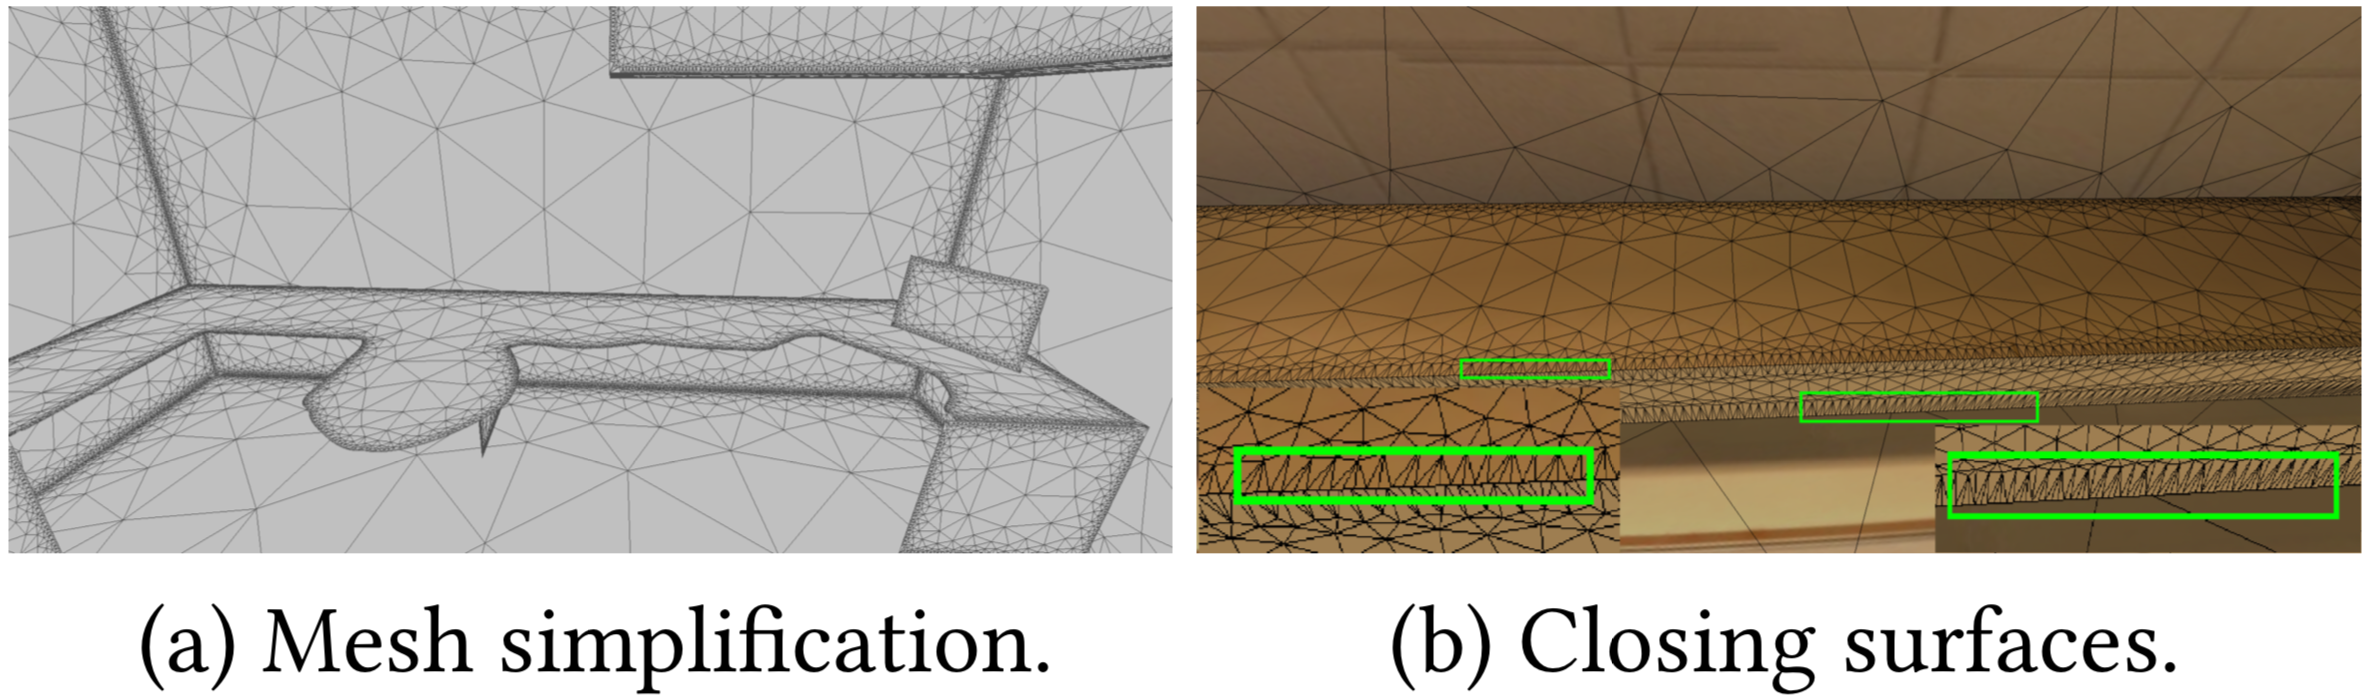
\includegraphics[width=0.8\linewidth]{3dlite/fig12.png}
\caption{Mesh simplification and vertex projection. (a) We simplify the planar primitives with constrained Delaunay triangulation. (b) We apply vertex projection to close the surfaces which should be connected.}
\label{fig:3dlite-remesh}
\end{figure}


\subsection{Results}
\label{sec:results}

We tested our method on a variety of RGB-D scans of indoor scenes.
All scans were captured using a \emph{Structure Sensor}\footnote{https://structure.io} mounted to an iPad Air, including several sequences from the BundleFusion data~\cite{dai2016bundlefusion} as well as the ScanNet~\cite{dai2017scannet} dataset.
We use $640\times 480$ color and depth, synchronized at $30$Hz.
Note that we are agnostic to the type of RGB-D sensor used.
For each scan, we compute the initial camera poses using BundleFusion. 
All 3DLite experiments  were performed on an Intel Core i7 2.6GHz CPU, with each scan taking on average 5 hours to process.
Detailed timings are shown in Table~\ref{table:3dlite-timing}.
\begin{table}
\center
\begin{tabular}{|c|c|c|c|c|c|}
\hline
& \multicolumn{3}{|c|}{BundleFusion Scenes} & \multicolumn{2}{|c|}{ScanNet}\\
\hline
Scenes & office0 & office1 & office3 & 0567\_01 & 0451\_05\\
\hline
Region(s) & 478 & 503 & 531 & 472 & 523\\
\hline
Plane(s) & 21.5 & 17.1 & 23.2 & 16.5 & 25.4\\
\hline
Sharpness(s) & 1138 & 1186 & 1266 & 811 & 8436\\
\hline
Color(s) & 11458 & 9553 & 14432 & 9866 & 9315\\
\hline
Boundary(s) & 1.156 & 1.101 & 1.157 & 0.781 & 1.384\\
\hline
\hline
& \multicolumn{3}{|c|}{ScanNet} & \multicolumn{2}{|c|}{other}\\
\hline
Scenes & 0294\_02 & 0271\_01 & 0220\_02 & apt & offices \\
\hline
Region(s) & 535 & 511 & 517 & 585 & 897\\
\hline
Plane(s) & 23.9 & 18.7 & 27.4 & 38.1 & 61.8\\
\hline
Sharpness(s) & 1011 & 828 & 935.4 & 1151 & 1968\\
\hline
Color(s) & 16407 & 9601 & 8575 & 18226 & 35976\\
\hline
Boundary(s) & 1.219 & 0.921 & 1.406 & 2.016 & 3.725\\
\hline
\end{tabular}
\caption{Timings (seconds) for different components.
}
\label{table:3dlite-timing}
\end{table}

\emph{Qualitative comparison.}
We first compare our lightweight, textured meshes of 10 scenes with 3D reconstructions computed using BundleFusion and VoxelHashing~\cite{niessner2013real}.
Note that since BundleFusion's online re-integration updates use color discretized to bytes, there may be some small color artifacts in the resulting reconstruction, so we first run BundleFusion to obtain camera poses and then compute a surface reconstruction with VoxelHashing.
As shown in Figs.~\ref{fig:3dlite-result-model} and \ref{fig:3dlite-result-tex}, even with simplified geometry, our high quality textures provide visually compelling results on completed scenes, drastically reducing various color oversmoothing artifacts.

\begin{figure}[!htb]
   \begin{minipage}{0.49\textwidth}
     \centering
	\includegraphics[width=\linewidth]{3dlite/fig13.png}
	\caption{Reconstructed meshes with high-quality surface textures. 
		3DLite produces completed scenes while significantly reducing color artifacts compared to reconstructions generated with BundleFusion~\cite{dai2016bundlefusion} and VoxelHashing~\cite{niessner2013real}.
	}
	\label{fig:3dlite-result-model}
   \end{minipage}\hfill
   \begin{minipage}{0.49\textwidth}
	\includegraphics[width=\linewidth]{3dlite/fig14.png}
	\caption{Zoomed-in views showing our reconstructed 3d models compared to reconstructions produced by BundleFusion~\cite{dai2016bundlefusion} and VoxelHashing~\cite{niessner2013real}.}
	\label{fig:3dlite-result-tex}
   \end{minipage}
\end{figure}


\emph{Primitive abstraction.}
We show several examples of our primitive-based geometry in Fig.~\ref{fig:3dlite-eval-plane}, which allows us to produce denoised and complete geometry compared to the original reconstruction, in a much more lightweight representation, which is more than 300 times smaller than the original mesh under the same resolution. The face number of our scenes is shown in Table~\ref{table:3dlite-face-num}.
\begin{table}
\center
\begin{tabular}{|c|c|c|c|c|c|}
\hline
& \multicolumn{3}{|c|}{BundleFusion Scenes} & \multicolumn{2}{|c|}{ScanNet}\\
\hline
Scenes & office0 & office1 & office3 & 0567\_01 & 0451\_05\\
\hline
FaceNum & 62559 & 68874 & 63479 & 43153 & 89621\\
\hline
\hline
& \multicolumn{3}{|c|}{ScanNet} & \multicolumn{2}{|c|}{other}\\
\hline
Scenes & 0294\_02 & 0271\_01 & 0220\_02 & apt & offices \\
\hline
FaceNum & 58709 & 58790 & 82864 & 92898 & 174200 \\
\hline
\end{tabular}
\caption{Number of faces in 3DLite models.
}
\label{table:3dlite-face-num}
\end{table}

\begin{figure}
\begin{minipage}{0.49\linewidth}
\centering
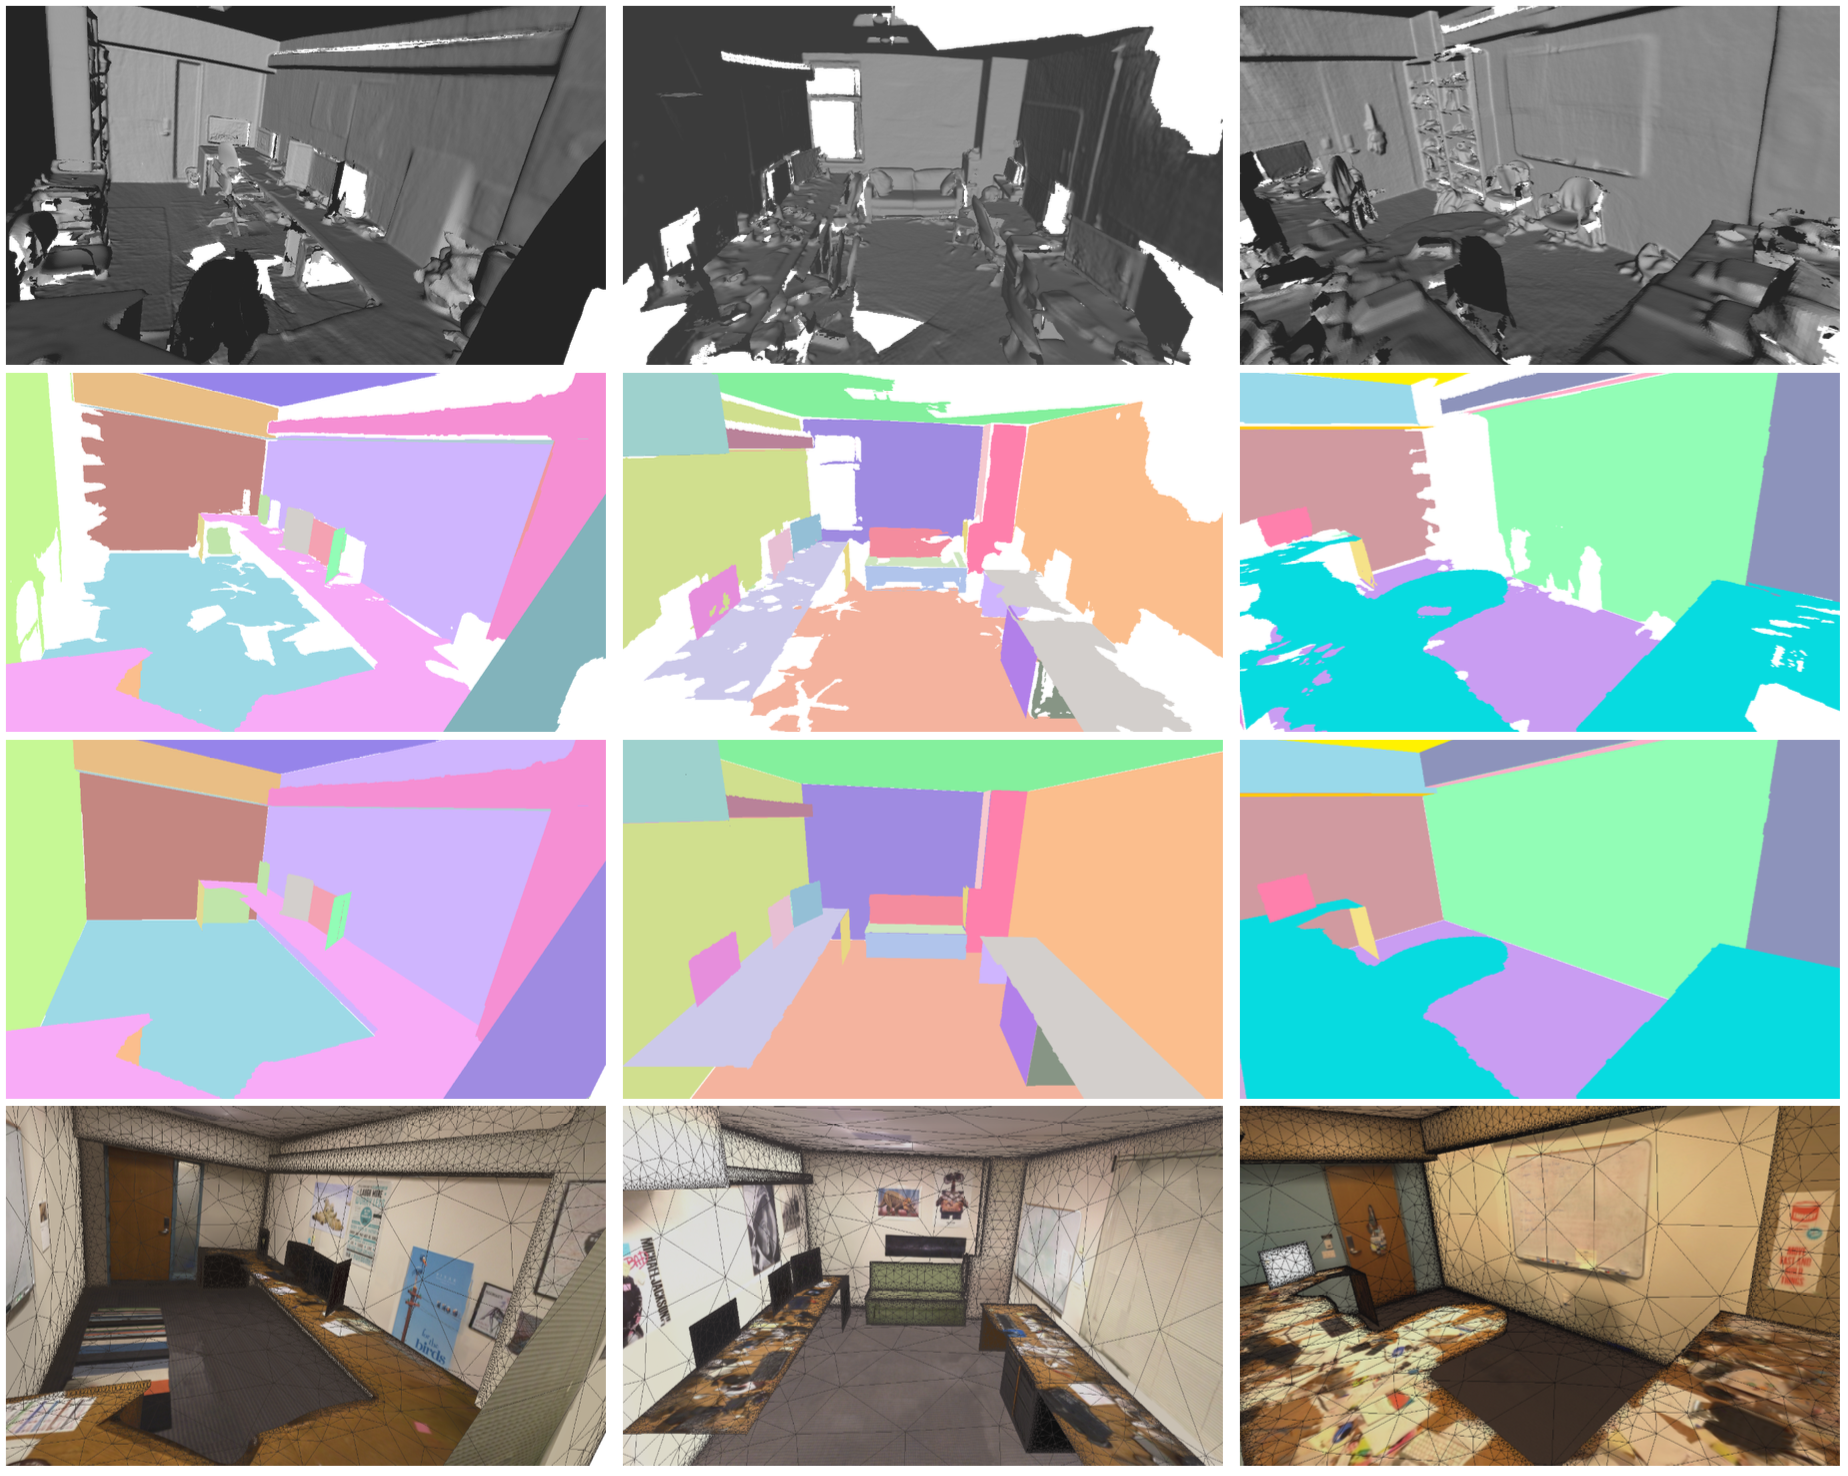
\includegraphics[width=\linewidth]{3dlite/fig15.png}
\caption{Primitive-based Abstraction. First row: original mesh. Second row: after primitive fitting. Third row: after geometry completion by primitive extrapolation. Last row: final result after texture mapping and mesh generation.}
\label{fig:3dlite-eval-plane}
\end{minipage}
\begin{minipage}{0.49\linewidth}
\centering
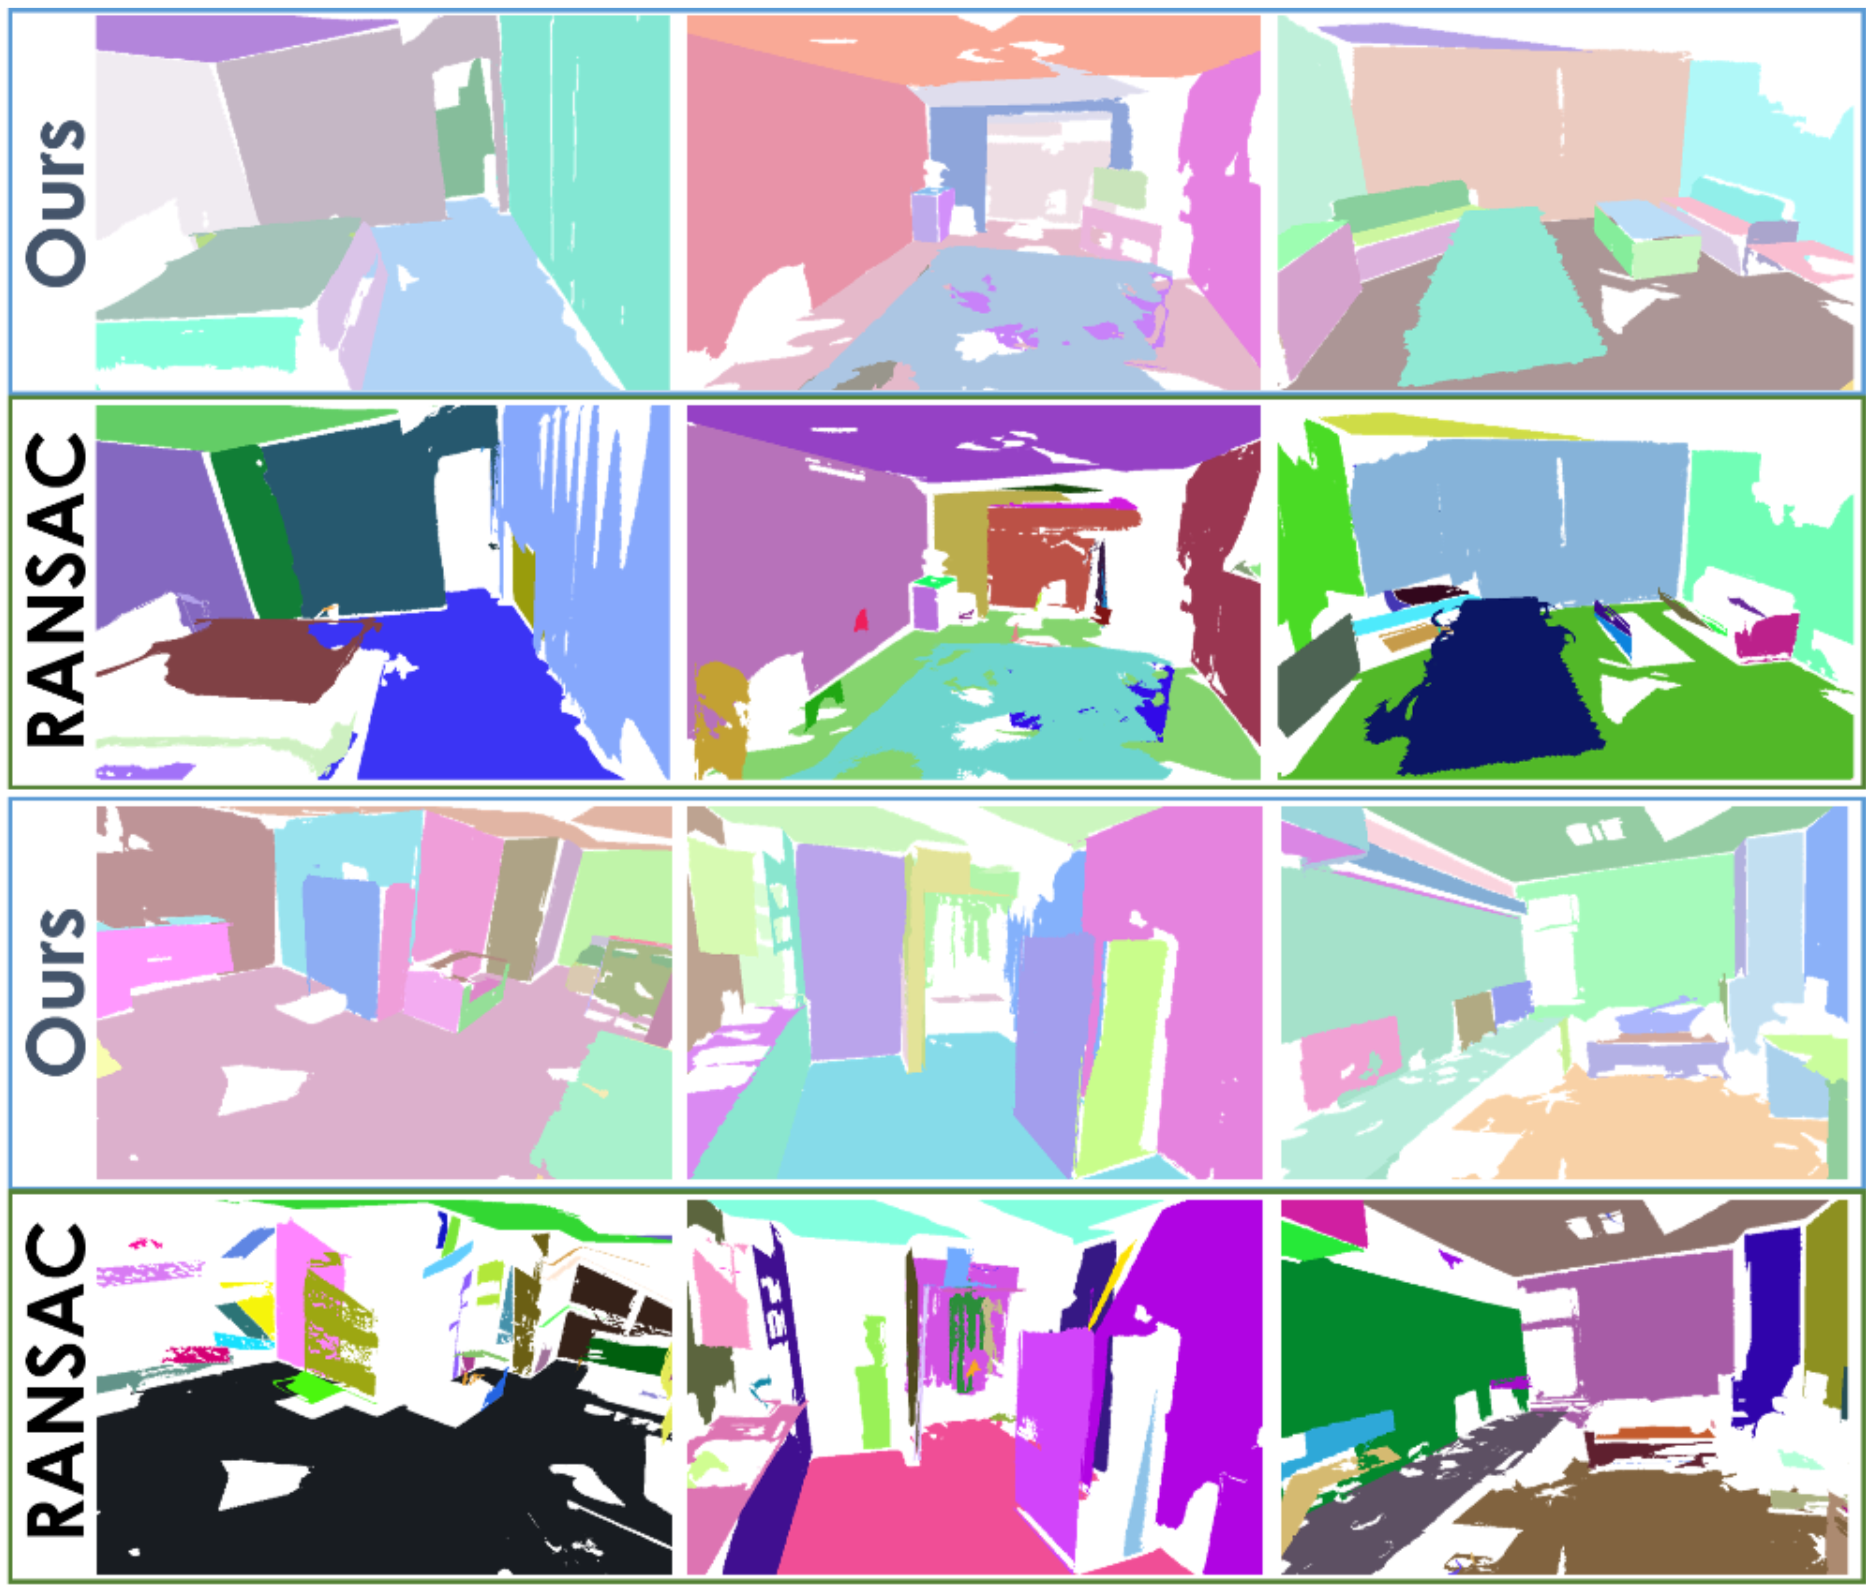
\includegraphics[width=\linewidth]{3dlite/fig16.png}
\caption{Comparison between our method and plane fitting with RANSAC.  Our method is more robust in detecting relatively small planes.}
\label{fig:3dlite-eval-fitting}
\end{minipage}
\end{figure}

Compared to traditional plane fitting using RANSAC, our method is more robust in detecting relatively small planes, as shown in Fig.~\ref{fig:3dlite-eval-fitting}.

\emph{Color alignment.}
We analyze our color alignment approach, showing the effect of our sparse and primitive geometry terms in Fig.~\ref{fig:3dlite-eval-align-rigid} (optimizing for rigid poses only).
Without color optimization, the result contains oversmoothing and ghosting. 
Optimizing for rigid poses under a dense photometric error using Zhou and Koltun~\cite{zhou2014color} sharpens the image but still retains some artifacts where initial camera poses were too far from the basin of convergence.
Our new terms are able to bring the optimization to a precise alignment of color frames.

\begin{figure}
\begin{minipage}{0.49\linewidth}
\centering
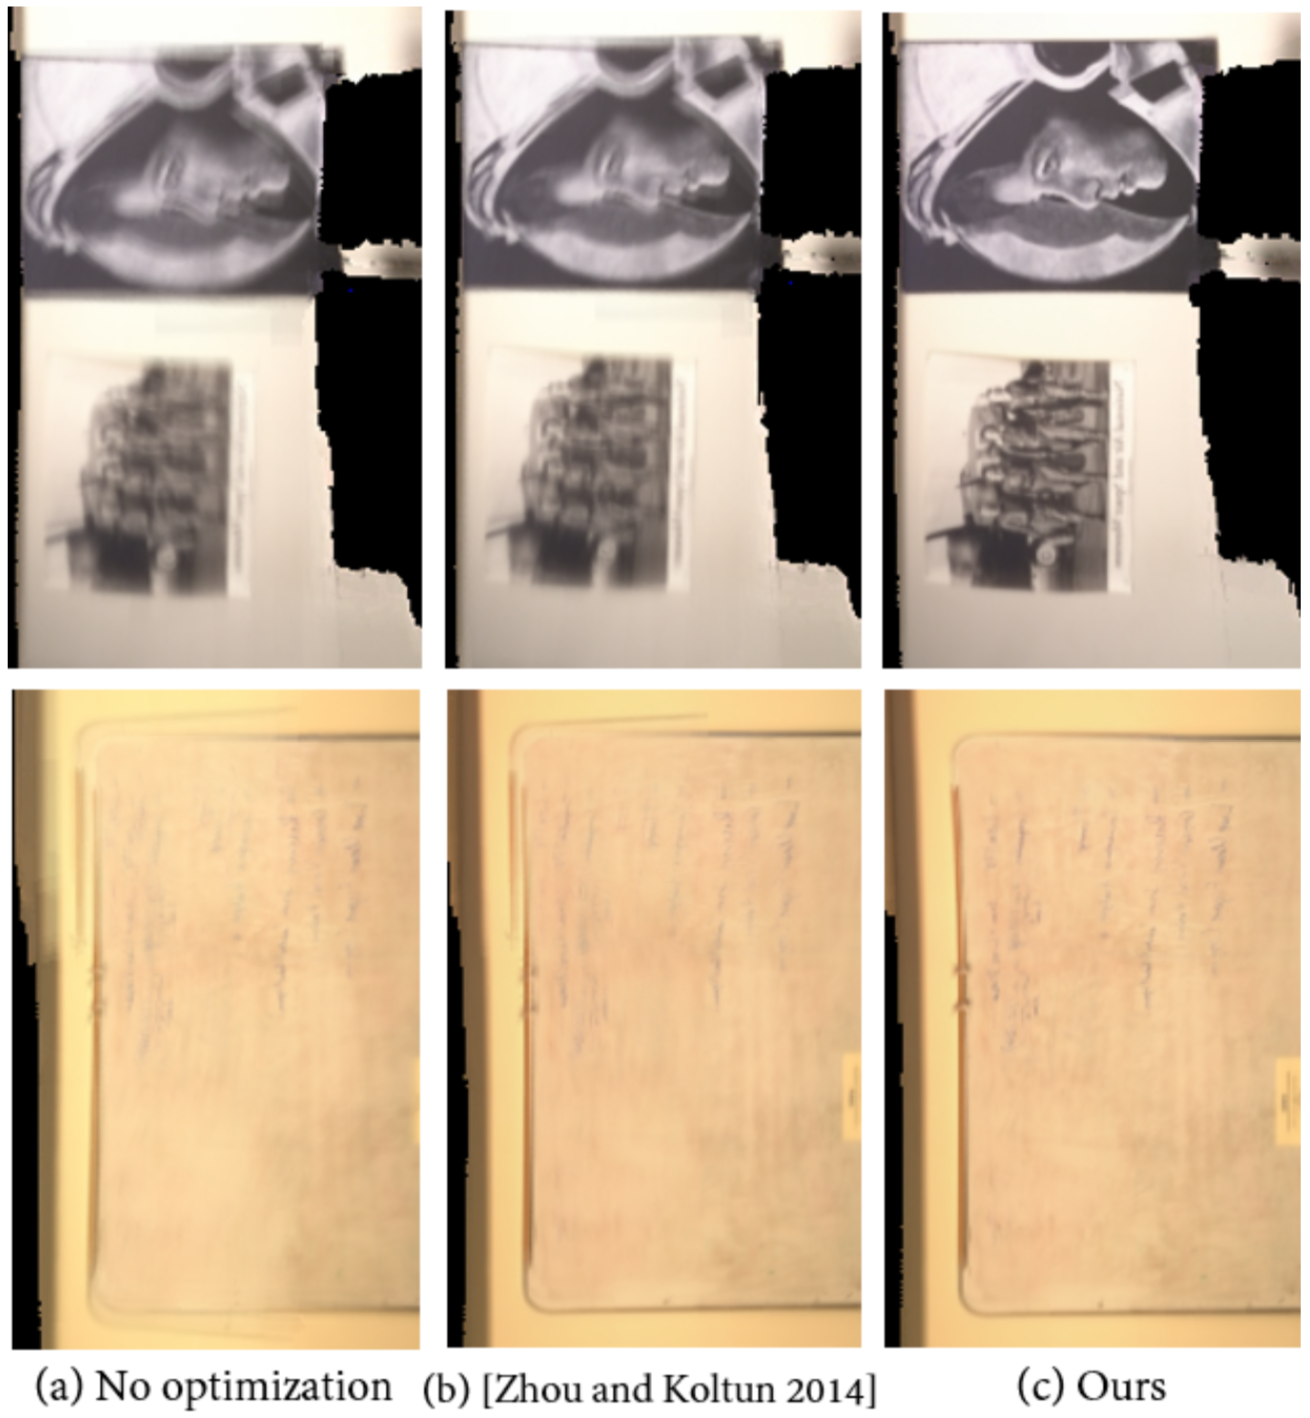
\includegraphics[width=\linewidth]{3dlite/fig17.png}
\caption{Color Alignment. (a) Color averaging. (b) Camera poses optimized with only dense color~\cite{zhou2014color}. (c) Camera poses optimized using our method, with dense color, sparse feature and geometry information.}
\label{fig:3dlite-eval-align-rigid}
\end{minipage}
\begin{minipage}{0.49\linewidth}
\centering
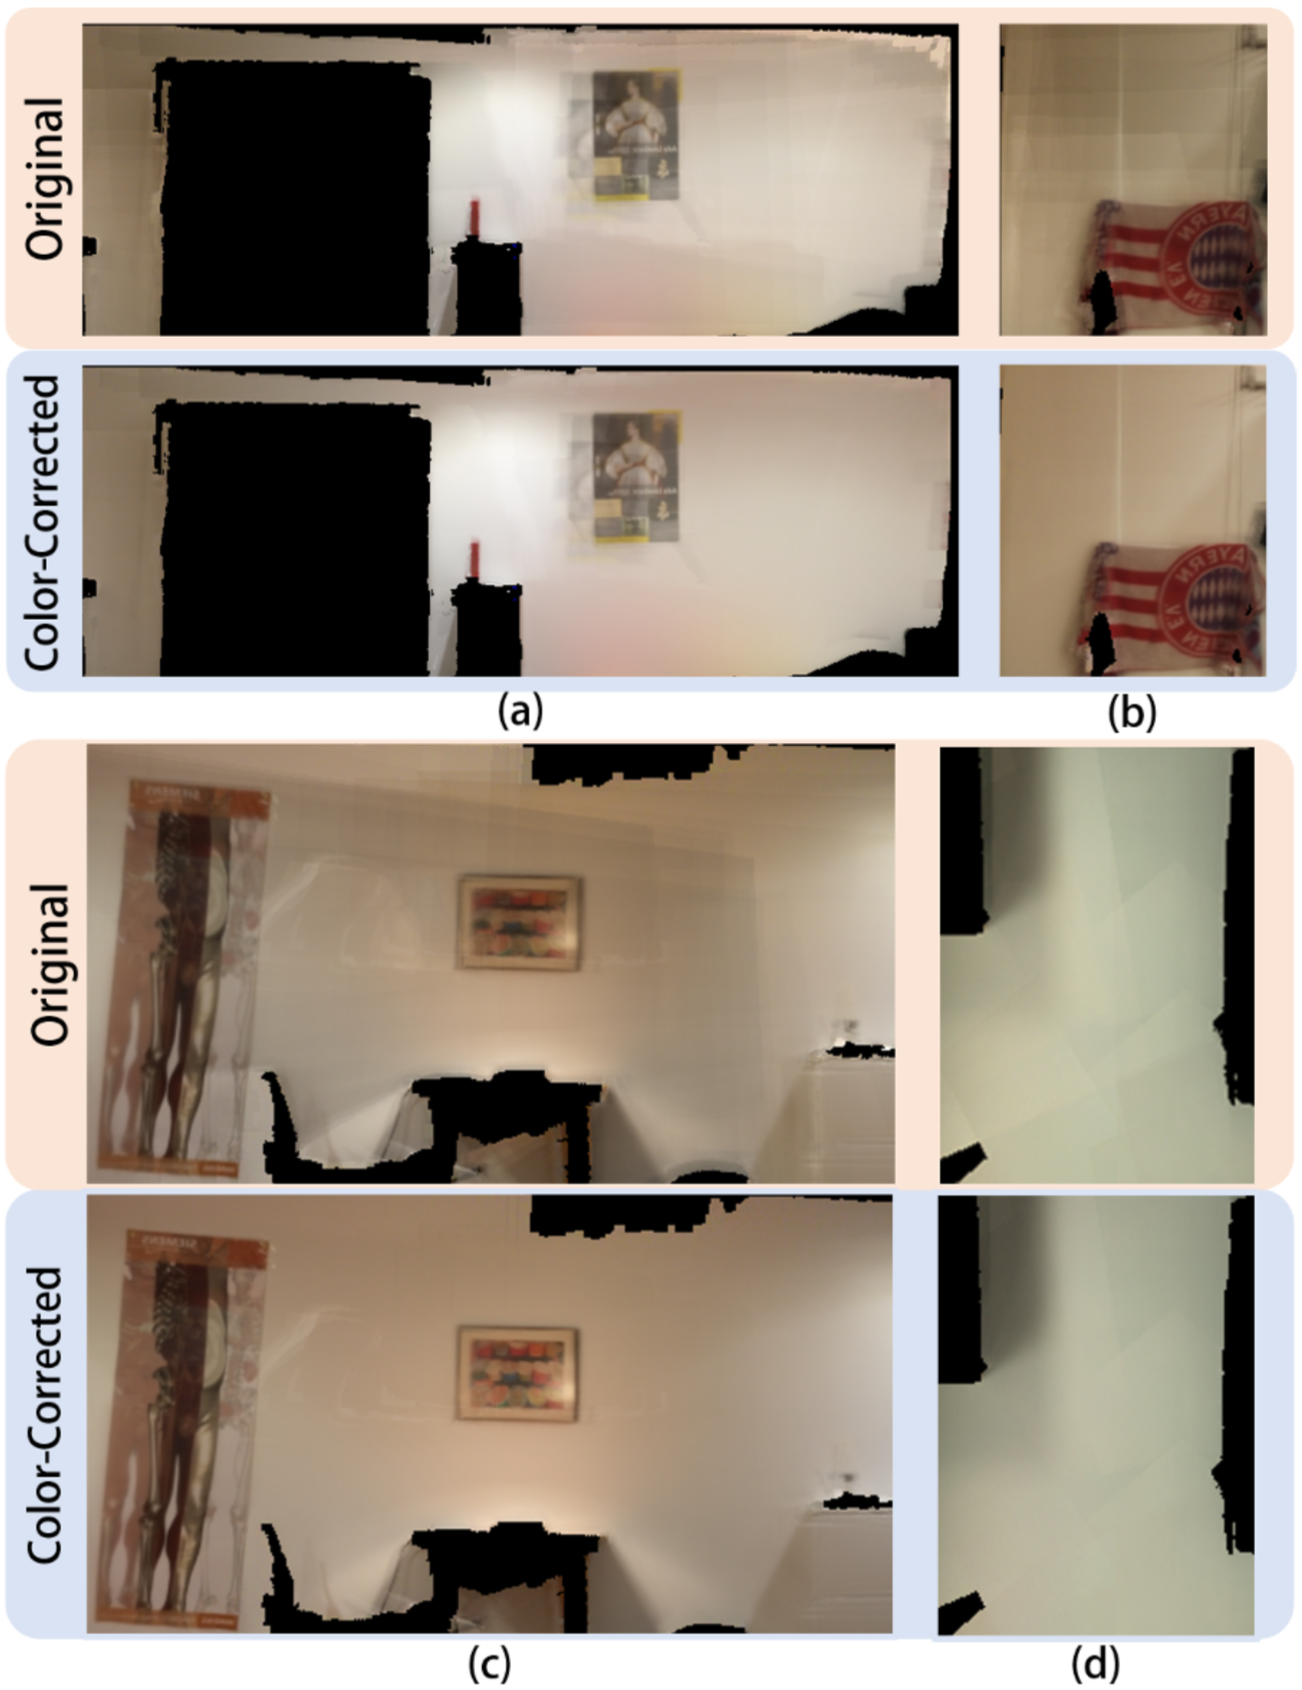
\includegraphics[width=0.8\linewidth]{3dlite/fig18.png}
\caption{Color transfer correction. (a)(b), and (d) are taken with auto exposure and white balancing, and (c) with fixed exposure and white balancing. Our color transfer optimization compensates for color inconsistencies in both scenarios. }
\label{fig:3dlite-eval-color-transfer}
\end{minipage}
\end{figure}

\begin{figure}
\begin{minipage}{0.49\linewidth}
\centering
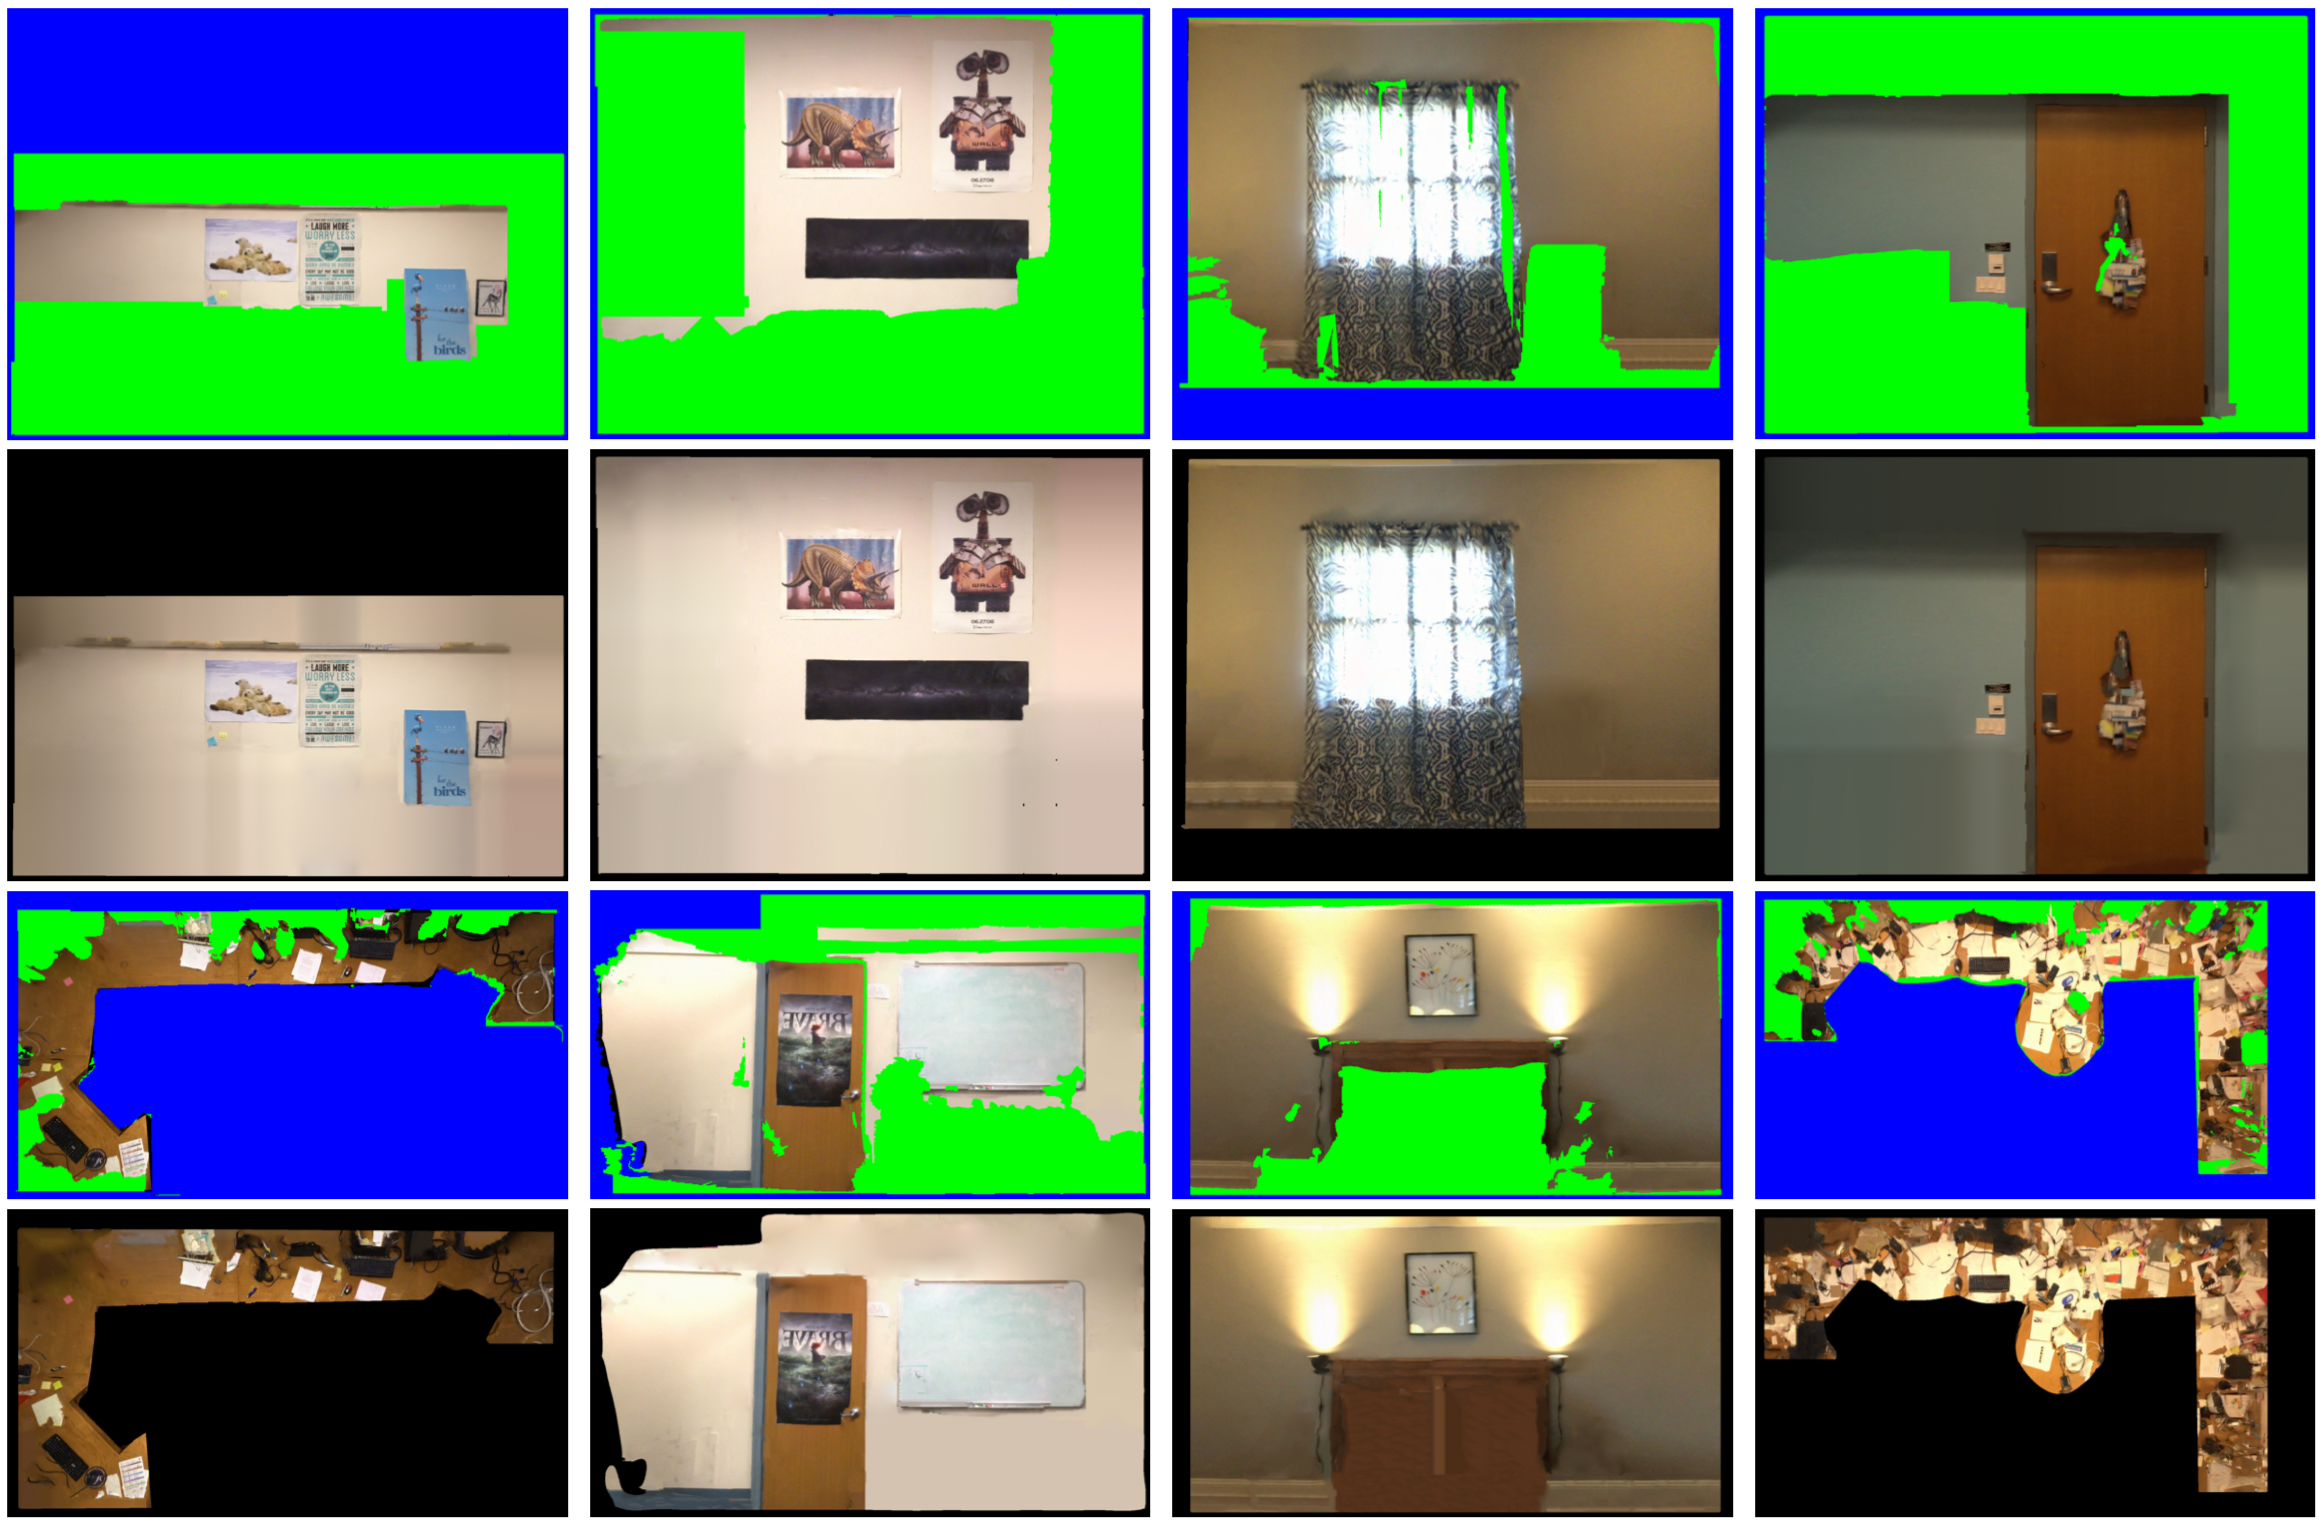
\includegraphics[width=\linewidth]{3dlite/fig20.png}
\caption{Texture completion using background filling with Image Melding~\cite{darabi2012image} to synthesize missing colors. Green represents unobserved regions to be synthesized, and blue empty space.}
\label{fig:3dlite-eval-complete}
\end{minipage}
\begin{minipage}{0.49\linewidth}
	\centering
    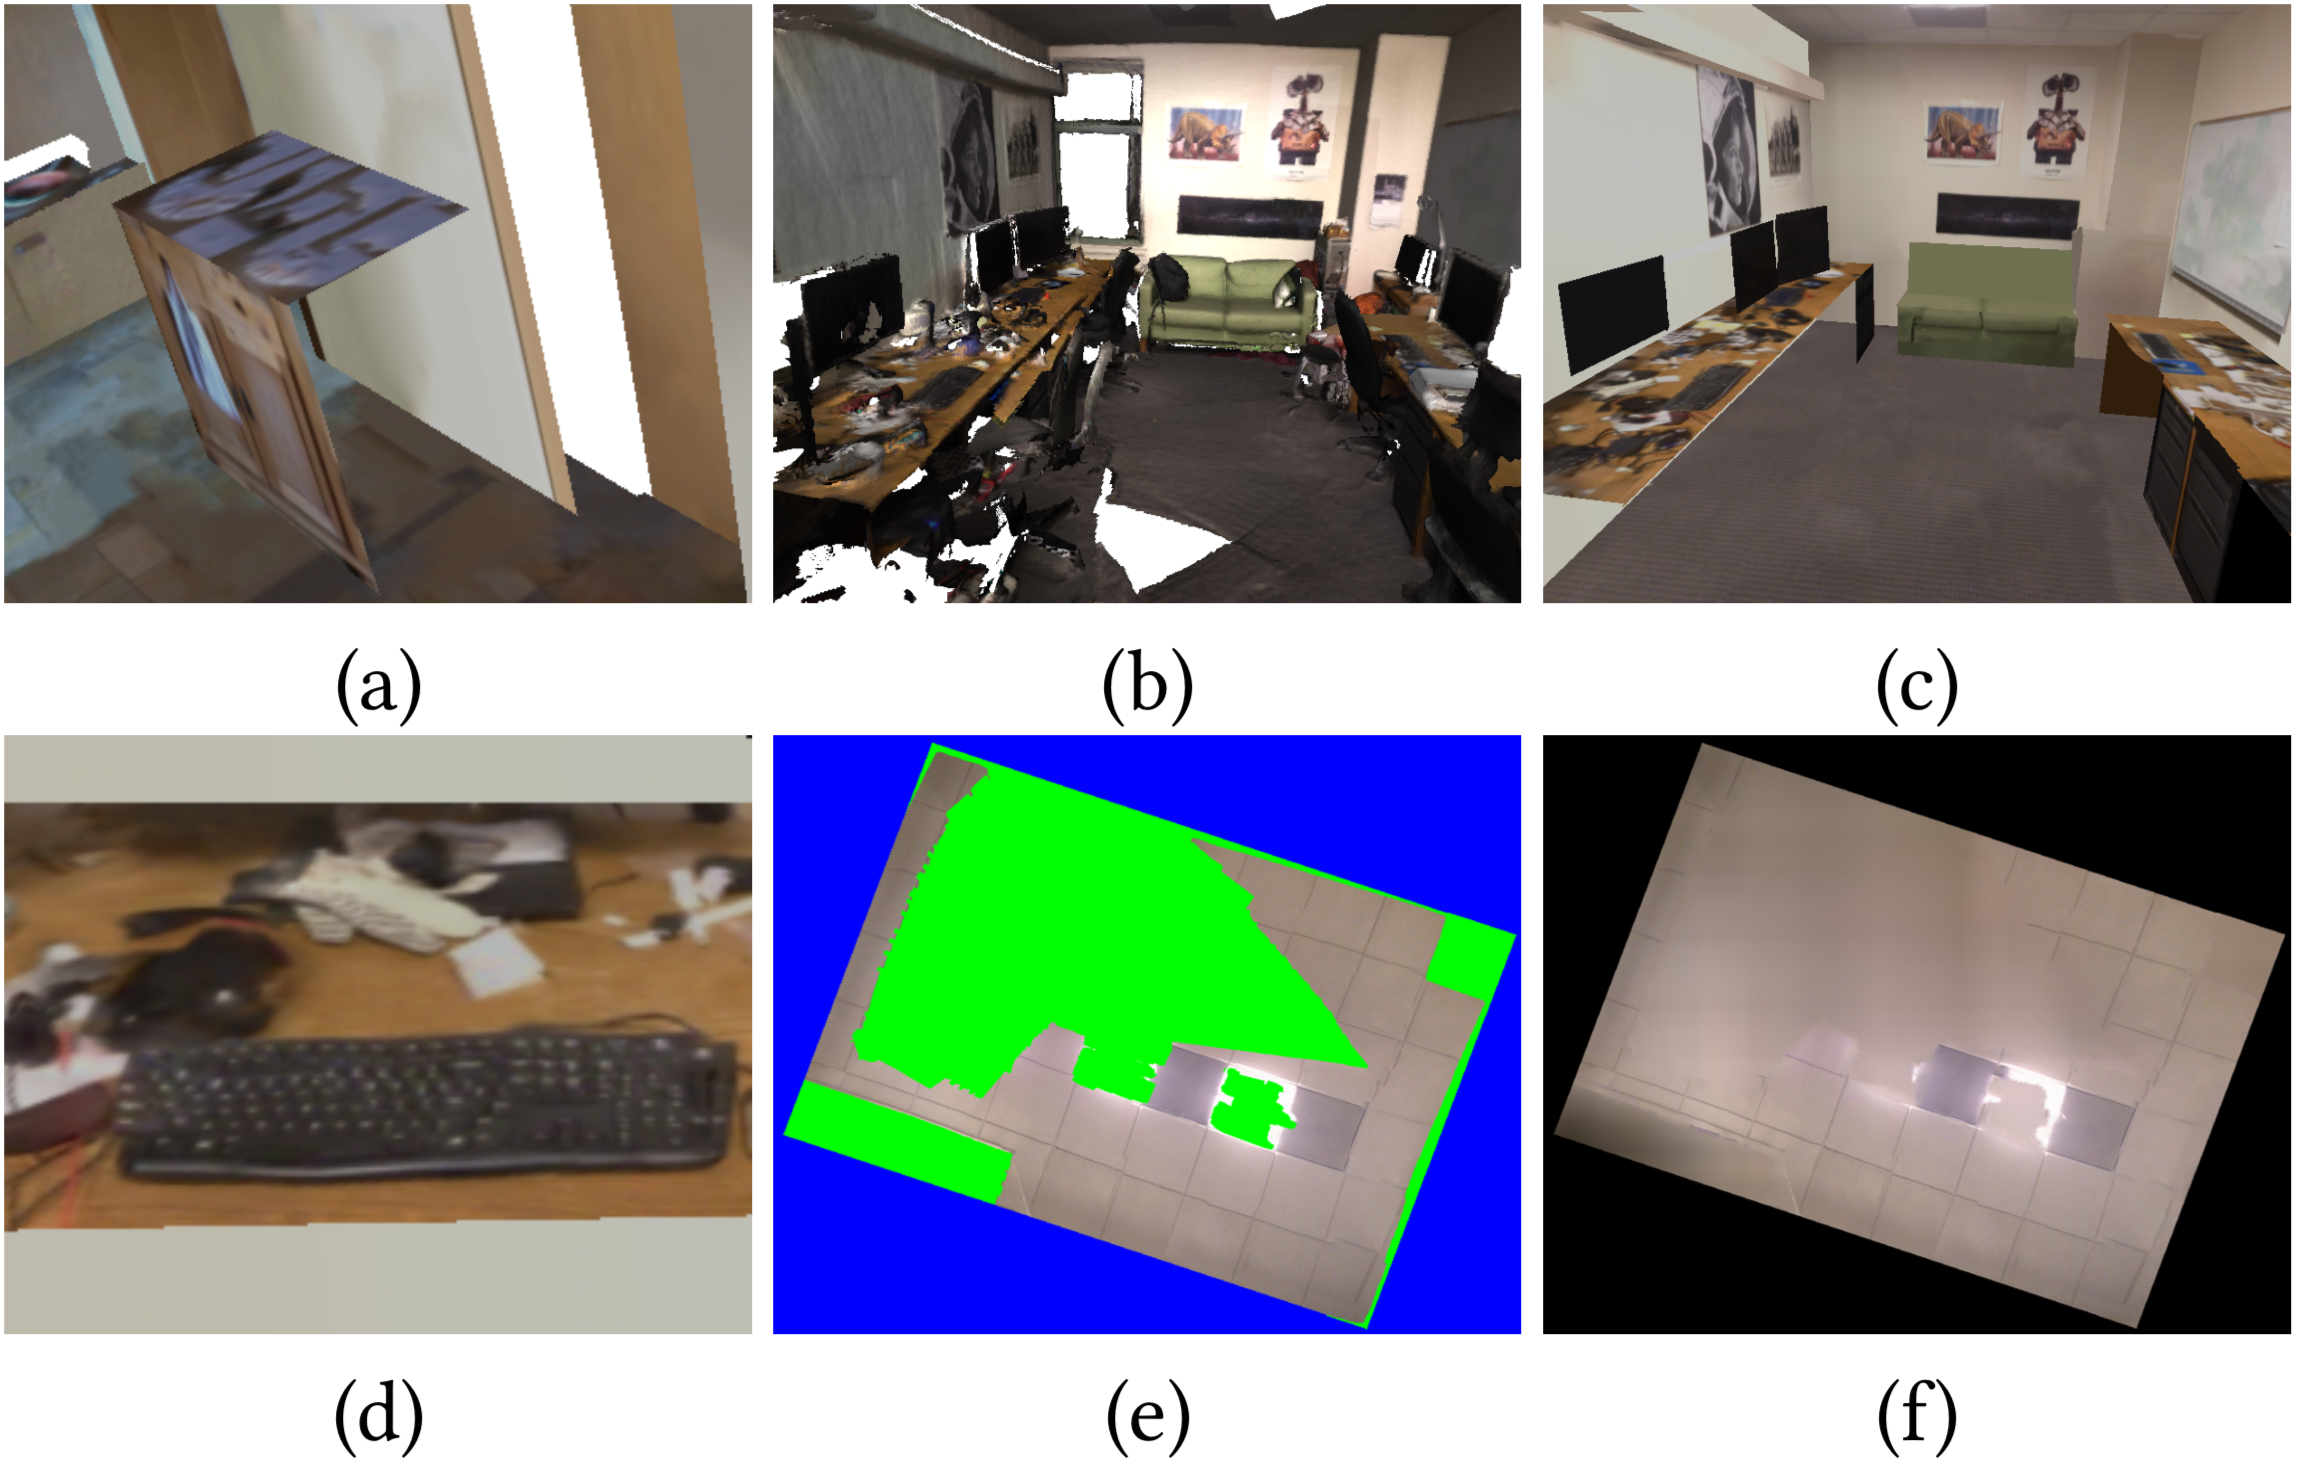
\includegraphics[width=\linewidth]{3dlite/fig21.png}
\caption{Limitations of our method. (a) Geometry entirely unseen in the original scan cannot be synthesized. (b-c) Non-planar objects (e.g., some chairs) are not captured by our current primitive abstraction. (d) Small objects may be projected onto planar surfaces, as the depth camera resolution is low. (e-f) Texture inpainting can have difficulty synthesizing large missing regions.}
	\label{fig:3dlite-limitation}
\end{minipage}
\end{figure}

\begin{figure}
\centering
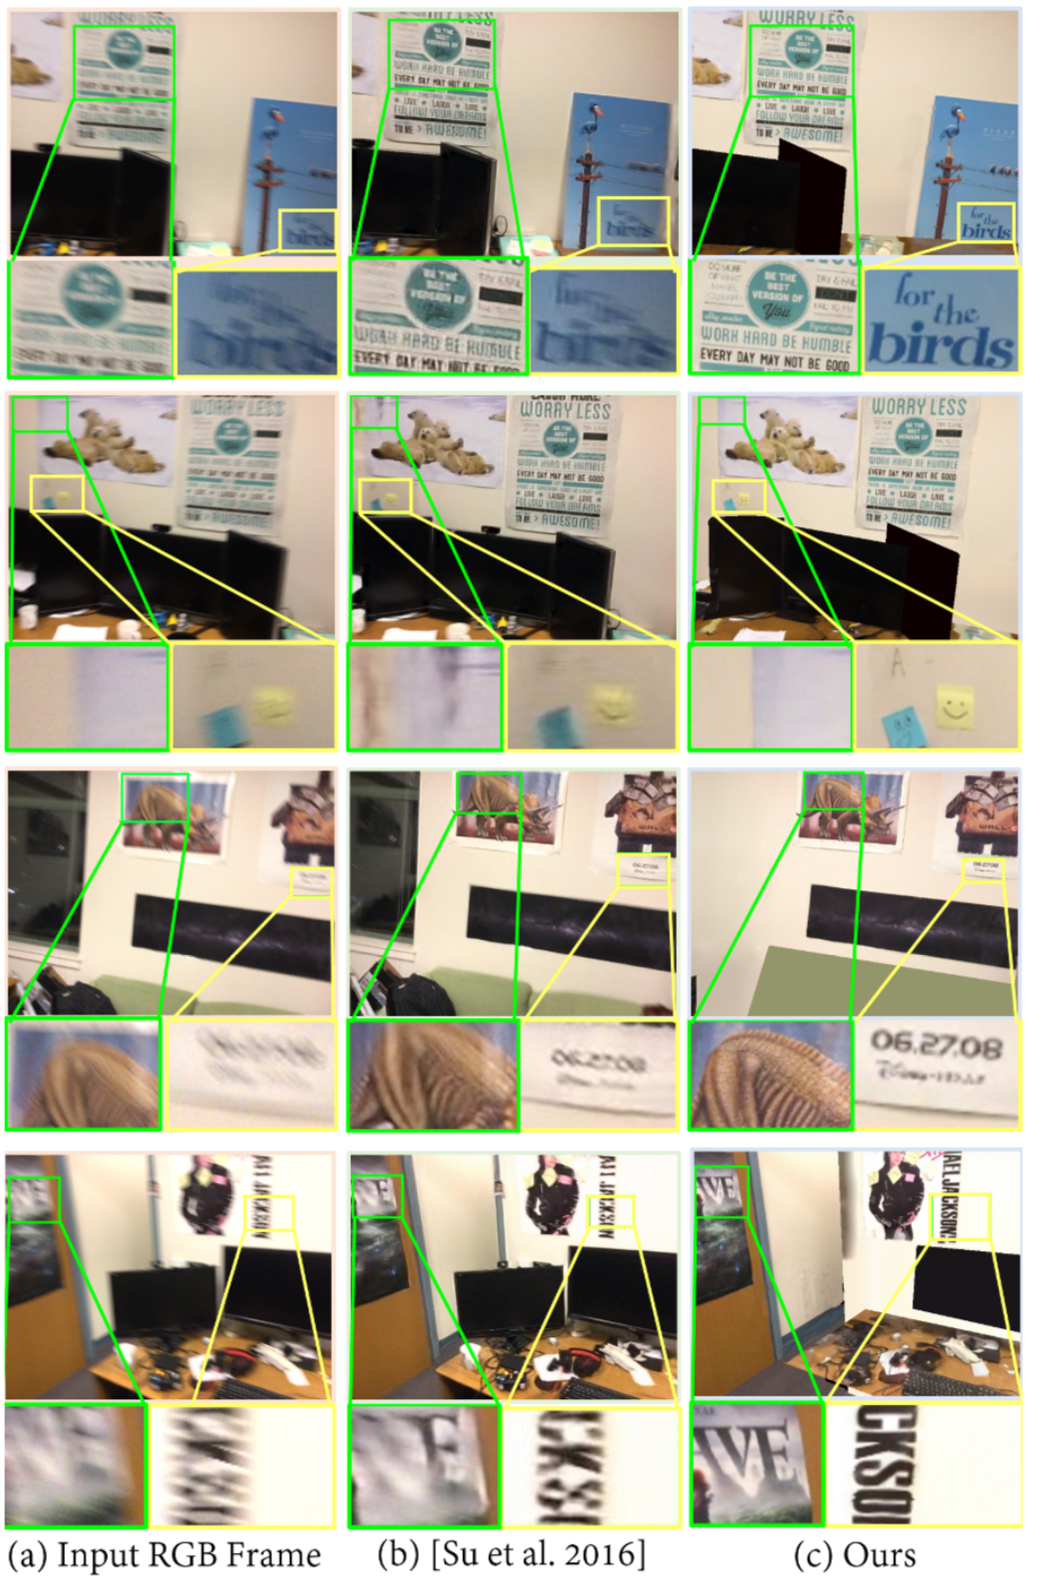
\includegraphics[width=\linewidth,height=1.2\linewidth]{3dlite/fig19.png}
\caption{Texture sharpening comparison. (a) Most input RGB frames are blurry. (b) Deep Video Deblurring~\cite{su2016deep} reduces some of the blur. (c) Our approach produces consistently sharp results.}
\label{fig:3dlite-eval-deblur}
\end{figure}

\emph{Color transfer correction.}
We show the effect of the color transfer optimization in Fig.~\ref{fig:3dlite-eval-color-transfer}, significantly reducing not only visible artifacts from auto-exposure and auto-white balancing, but also various color inconsistencies which can occur even under fixed exposure and white balancing settings.

\emph{Texture sharpening.}
In Fig.~\ref{fig:3dlite-eval-deblur}, we show the effectiveness of our texture sharpening approach.
Since we generate a consistent texturing from sharp regions of the input images, images rendered from our 3D model can be sharper than some of the original RGB images (which often contain motion blur), as well as deblurred RGB images using advanced video motion deblur techniques~\cite{su2016deep}.
Such deblurring, while noticeably reducing blur in several parts of the image, still has some difficulty near image boundaries, and with large motion.

\emph{Texture completion.}
Fig.~\ref{fig:3dlite-eval-complete} shows several texture completion results using background filling along with Image Melding~\cite{darabi2012image} to synthesize colors in unobserved regions.
We are thus able to generate complete scene models with textured geometry.

\subsection{Limitations}
\label{subsec:3dlite-limitations}

While 3DLite can robustly generate lightweight, abstracted models with sharp textures, it still suffers from several limitations, as visualized in Fig.~\ref{fig:3dlite-limitation}.
If there is geometry entirely unseen in the original scan, we cannot generate it from scratch to complete these regions. 
Additionally, small objects (e.g., keyboards, mice) are often projected onto planar primitives; this is not too dissimilar from reconstructions generated from volumetric fusion, where the coarse resolution, noise, and distortion of a commodity depth sensor can also make small objects difficult to distinguish geometrically.
Further, while state-of-the-art texture synthesis methods can achieve impressive results, they are not perfect, and may still have difficulty synthesizing color in large missing regions.
Most notably, our current primitive abstraction is plane-based, so relatively non-planar objects (e.g., some chairs) are not captured in our geometric abstraction. We hope to extend our approach in combination with CAD model retrieval, alignment, and texturing in order to retain all scene geometry and texture.

\section{Adversarial Texture}
\label{sec:tadv}
\subsection{Method}

\begin{figure*}
    \centering
    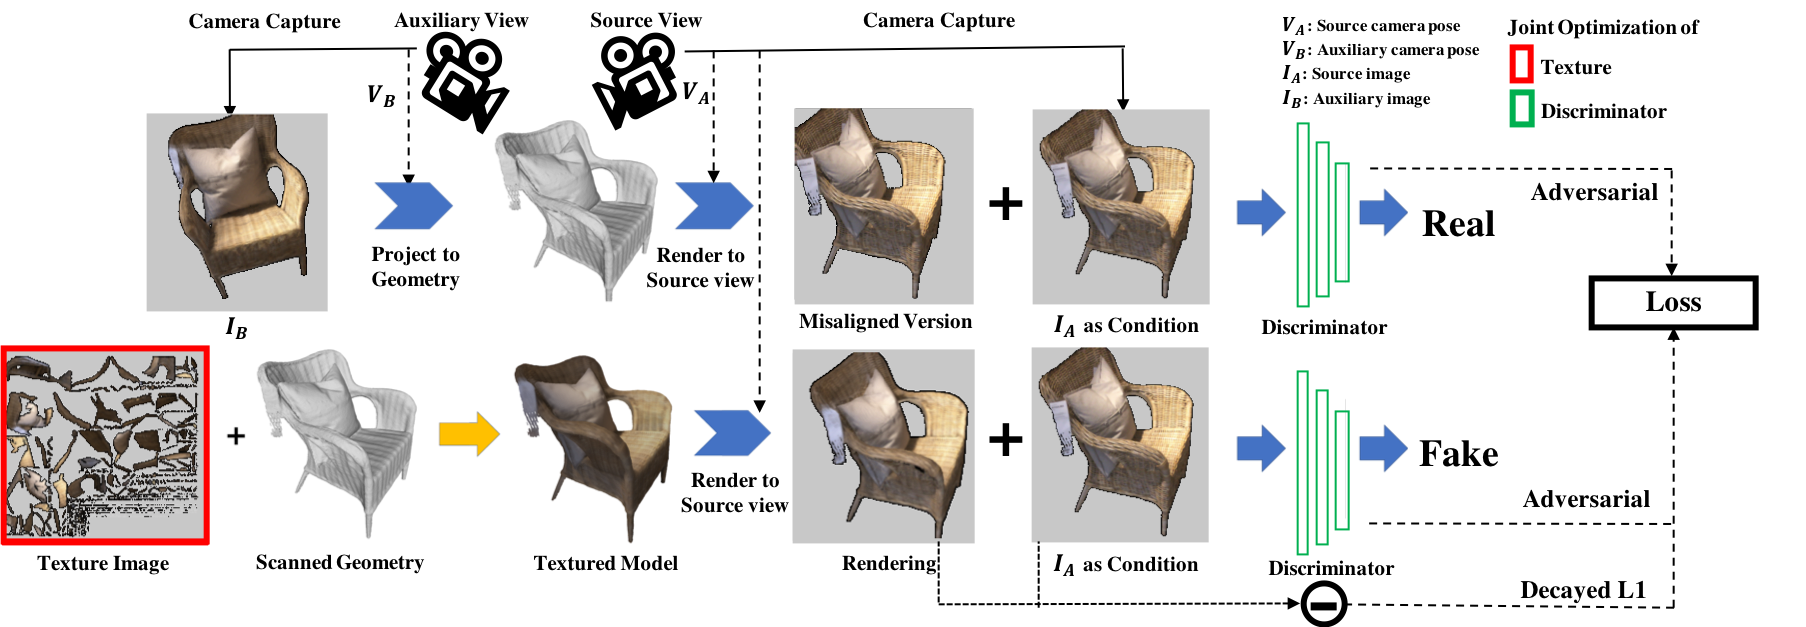
\includegraphics[width=\linewidth]{texturegen/figures/pipeline.png}
    \caption{Texture Generation. 
    From an input RGB-D scan, we optimize for both its texture image and a learned texture objective function characterized by  a discriminator network. 
    The discriminator operates on reprojections of input color images in order to maintain robustness to various misalignments.
    We randomly pick a pair of input images, \emph{source} and \emph{auxiliary}, and synthesize the fake and real examples from the source view, conditioned on the re-projected source image. 
    The texture image and discriminator are trained in an alternating process.}
    \label{fig:toptim-pipeline}
\end{figure*}

Our goal is the optimization of a color texture that can be used to render a scanned scene using a classical computer graphics pipeline.
%
During the scanning procedure, we obtain color images and their estimated camera poses.
%
These views, along with the reconstructed geometry, are input to our method.
%
To optimize for a color texture, we must specify an objective function; in this case, we need to account for misalignments of the color images and the reconstructed model.
%
To this end, we propose to learn the loss function in conjunction with the texture (see Figure~\ref{fig:toptim-pipeline}).
%
The function is modeled as an adversarial loss using a discriminator network identifying `real' and `fake' imagery, and is designed to provide a misalignment-tolerant metric for our texture optimization.
%

\subsection{Misalignment-Tolerant Metric}
\label{sec:approach-misalign}



%
Our key insight is to propose to learn a conditional discriminator as a misalignment-tolerant metric adaptive to the error distribution of the input data.
%
Figure~\ref{fig:toptim-misalign-example}(a) shows a 2D example where two observations (b) and (c) are misaligned by 2 units in the horizontal directions, and an L2 loss results in blurry appearance.
%
Ultimately, we aim to synthesize a texture that appears as realistic as either observation.
%
To achieve this, we ask the discriminator to consider both (b) and (c) as real conditioned on either observation.
%
With such a discriminator, the blurred (d) results in a large loss and the texture will instead converge to either (b) or (c).
%

%
We extend this intuition to 3D where the geometry is observed from different viewpoints.
%
We then aim to optimize a texture such that local patches of the texture rendered to various views look realistic.
%
Therefore, conditioned on any arbitrary view, we generate real examples by a re-projection from any other view to this view, as shown in Figure~\ref{fig:toptim-pipeline}.
%
Such re-projection can be achieved by projecting the color image onto the surface and then rendering back to another view.
%
Unlike the simple 2D example, it is highly possible that there is no texture solution so that each local patch perfectly matches the one view from the input images, given camera and geometry error.
%
However, the proposed approach is expected to push those inconsistencies to the smooth textured regions to hide any artifacts that can be easily identified by the discriminator, and thereby producing locally consistent realistic texture solution.
%

%
For each optimization iteration, we randomly select two input images, $I_A$ (source image) and $I_B$ (auxiliary image) with corresponding camera poses $V_A$ and $V_B$.
%
The conditioning is $I_A$ from the viewpoint $V_A$, and the `real' image is $I_B$ projected to the scan geometry and rendered from $V_A$, while the `fake' image is the synthesized texture rendered from $V_A$.
%
We alternating optimize the texture and discriminator.
%
During texture optimization, we adjust the texture pixel colors to maximize the adversarial loss such that it looks more realistic under the discriminator scoring.
%
During discriminator optimization, we minimize the adversarial loss such that it better classifies real and fake examples.
%
We linearly combine adversarial loss with an L1 loss that decays exponentially as the optimization proceeds, which helps the optimizer find a good initial texture solution.
%


\begin{figure}
    \centering
    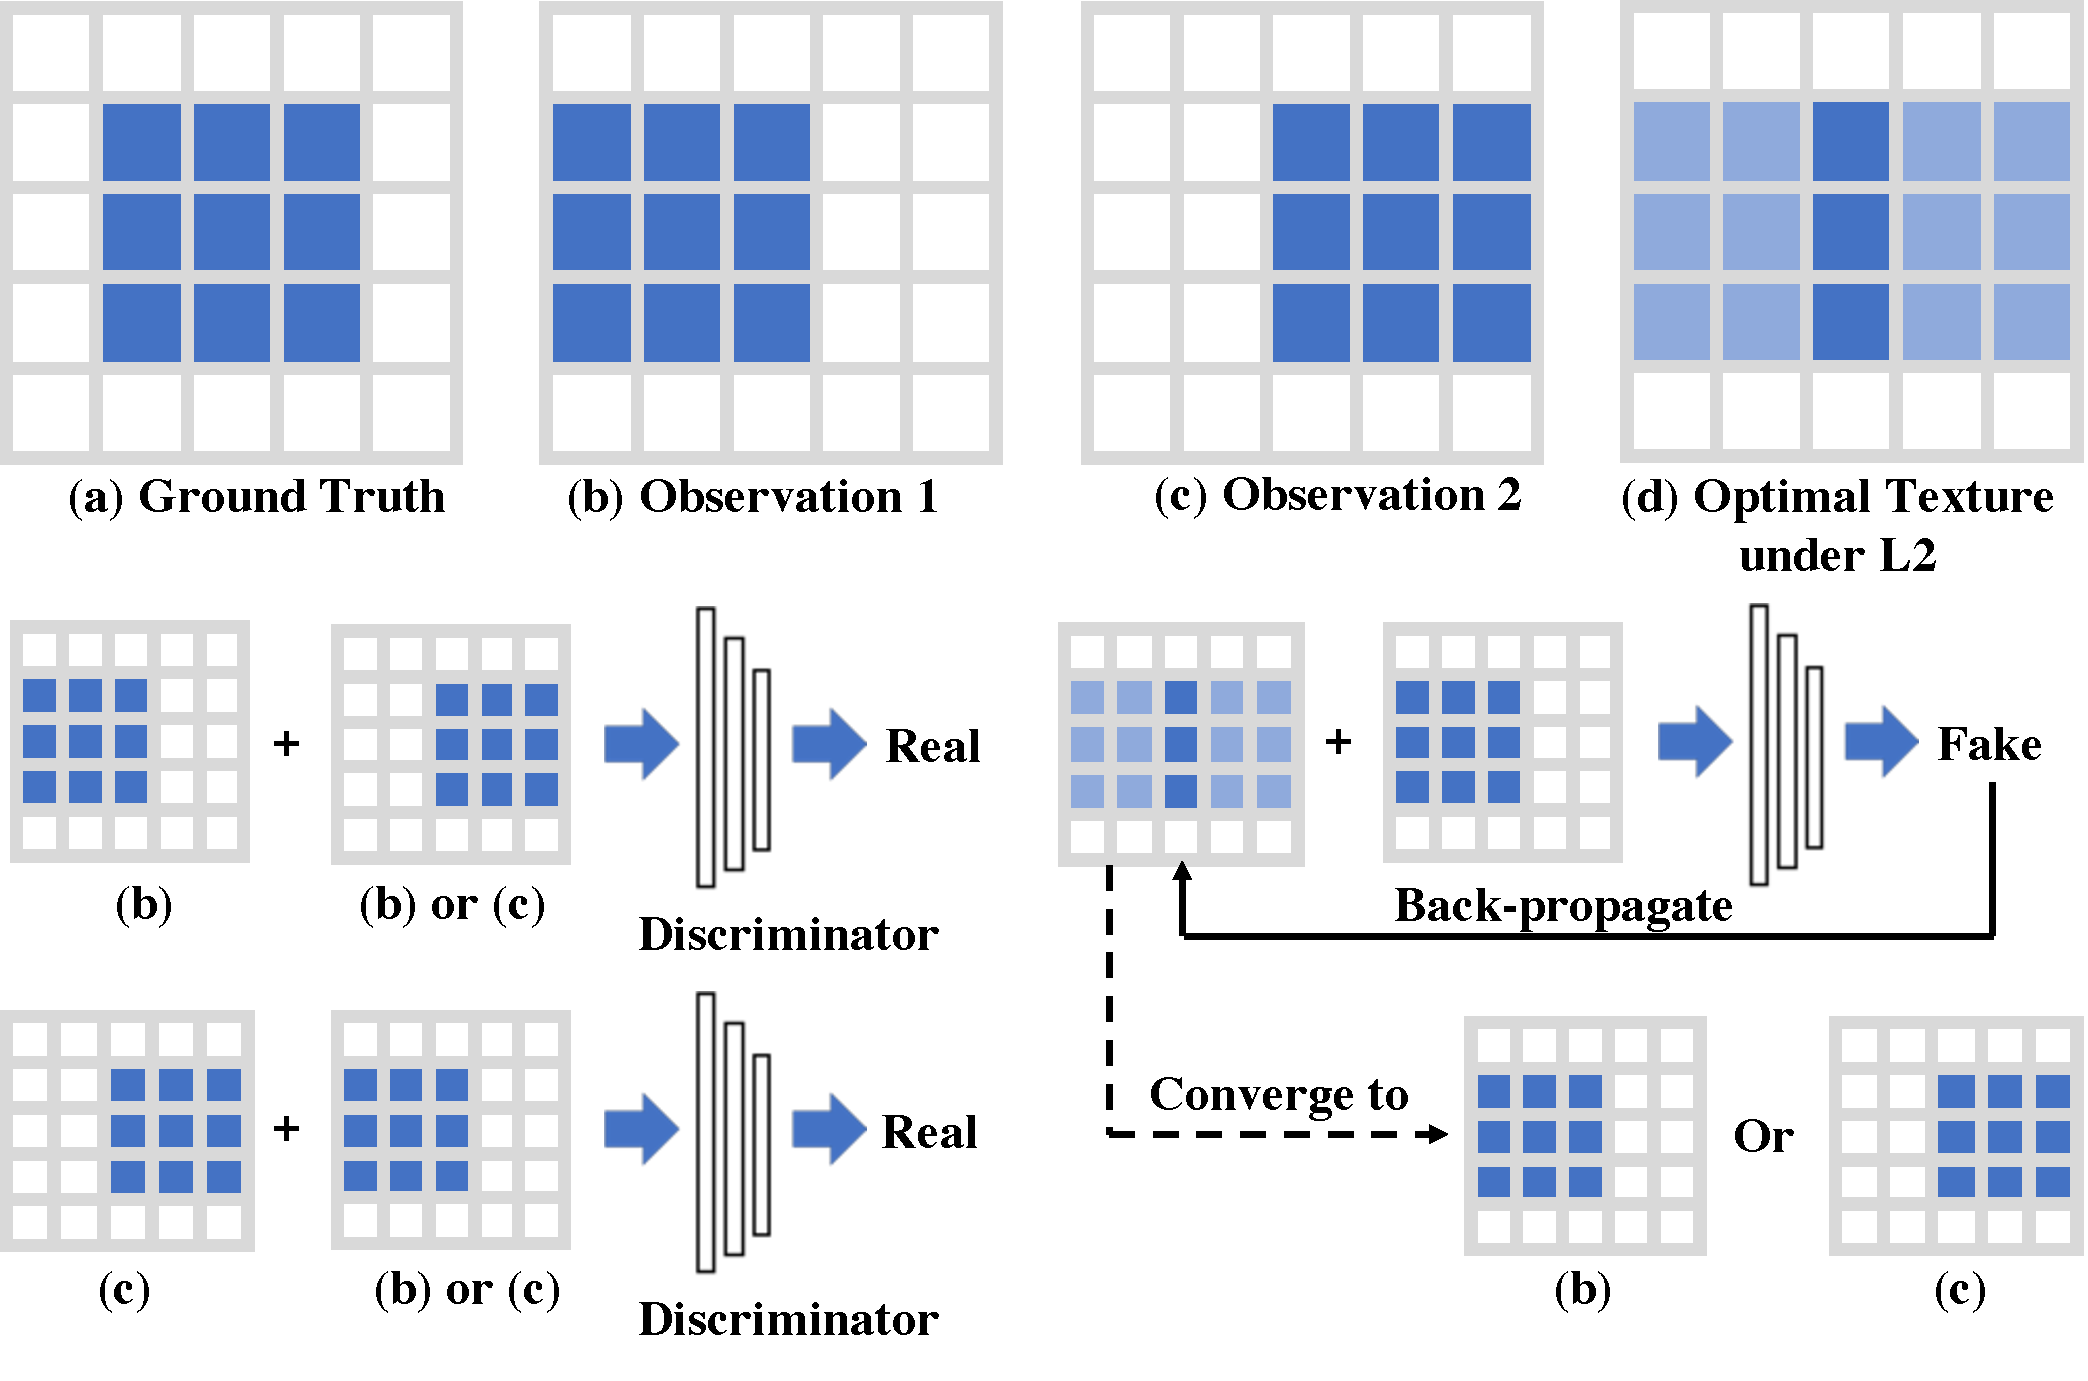
\includegraphics[width=0.75\linewidth]{texturegen/figures/intuitive.pdf}
    \caption{2D example of a misalignment. (a) shows the ground truth pattern, which is observed with misalignment in (b) and (c); an L2 loss results in blurring (d). 
    We train a discriminator which only accepts (b) and (c) as real examples conditioned on each other, and use it to optimize the texture, which converges to either (b) or (c).}
    \label{fig:toptim-misalign-example}
\end{figure}

\paragraph{Network Architecture}
%
Our framework is adopted from the PatchGAN discriminator architecture proposed by Isola et al.~\cite{isola2017image}.  We choose that framework because it is designed to produce local details that look as realistic as a given set of input images.
%
We use three convolutional layers, resulting in a patch size of $70\times 70$, which we find suitable for our input images of resolution $640\times 480$.
%
Unlike the original, we remove all batch normalization layers and feed a single view example for each optimization iteration, which we empirically found to improve performance.
%
Conditioned on the input view, we ask the discriminator to evaluate the residual of the synthesized example subtracted by the condition input.
%
Finally, since we focus on evaluating foreground regions (pixels corresponding to input geometry), we remove the loss terms for regions where background comprises more than $90\%$ of the receptive field.
%

%\subsection{Conditional Adversarial Loss}
\subsection{Texture Optimization}% of the Texture and the Metric}

%
To retrieve a texture, we jointly optimize the texture and the misalignment-tolerant metric.
%The texture and the misalignment-tolerant metric is learned jointly.
%
Inspired by the adversarial loss used in Pix2Pix~\cite{isola2017image}, we express our view-conditioned adversarial loss as:
\begin{align}
\begin{split}
    \mathcal{L}_c(T,D) &= \mathbb{E}_{x,y}(\log D(x,y)) +\\ &\mathbb{E}_{x,M_x}(\log (1 - D(x, M_x(T) ) ),
\end{split}
\end{align}
where $T$ and $D$ represent the target texture image and the discriminator parameters we are optimizing for.
%
$x$ is the condition, a reprojected color image from the input sequence of captured images.
%
$M_x$ is the fixed texture-to-image mapping given the camera pose associated with $x$. 
%
Here, a real example is an image $y$ re-projected to the view of $x$.
%
We optimize $D$ with the objective to correctly identify real examples, misaligned real imagery, and fake examples rendered from the texture as $M_x(T)$. 
%
Simultaneously, we optimize the texture $T$ such that it is difficult to be identified as fake when mapped to view of $x$.
%

%
Since the adversarial loss alone can be difficult to train, we additionally add an L1 loss to the texture optimization to provide initial guidance for the optimization:
%
\begin{equation}
\mathcal{L}_{L1}(T) = \mathbb{E}_{x,y,M_x} ||y - M_x(T)||_1.
\end{equation}
Our objective texture solution is:
\begin{equation}
    T^* = \arg \min_{T} \max_{D} \mathcal{L}_c(T,D) + \lambda \mathcal{L}_{L1}(T).
\end{equation}

%
During training, we initialize all pixels in texture image to zero and $\lambda=10$.
%
The high $\lambda$ allows the L1 loss to provide an initial texture, and for every 1000 steps we exponentially decay the lambda by a factor of $0.8$.
%
We optimize in alternating fashion for each optimization step, using the Adam optimizer for both the texture and discriminator with learning rates $10^{-3}$ and $10^{-4}$ respectively.
%
For each object or scene, we optimize for 50000 steps to finalize our texture. 
%

\subsection{Differentiable Rendering and Projection}
%
%In the fake example synthesis, we need to render the texture into the view together with the gradient information.
To enable the optimization of the RGB texture of a 3D model, we leverage a differentiable rendering to generate synthesized `fake' views.
We pre-compute a view-to-texture mapping, and can then implement the rendering with a differentiable bilinear sampling layer. 

To create the misaligned `real' images ($I_B$ seen from $V_A$), we compute a reprojection; note that here we do not need to maintain gradient information.
For each pixel $\mathbf{P}_A$ in the source image, we need to determine the corresponding pixel $\mathbf{P}_B$ in the auxiliary image, so that a bilinear sampling can be applied to warp image from the $V_B$ to $V_A$. 
Specifically, for $\mathbf{P}_A$ with depth value $d_A$ from the source depth map, we can determine its 3D location in the source view's space as $\mathbf{p_A}=d_A\mathbf{K}^{-1}\mathbf{P_A}$ where $\mathbf{K}$ is the intrinsic camera matrix. 
Suppose the transformations from the camera to the world space for the source and the auxiliary views are given as $\mathbf{T}_A$ and $\mathbf{T}_B$, the corresponding 3D and pixel location in the auxiliary view are $\mathbf{p}_B=\mathbf{T}_B^{-1}\mathbf{T}_A\mathbf{p_A}$ and $\mathbf{P}_B=\mathbf{K}\mathbf{p}_B$. 
The pixel is visible in the auxiliary view if $\mathbf{P}_B$ is in the scope of the image and the difference between z-dimension of $\mathbf{p}_B$ and $d_B$ from the auxiliary depth map is smaller than a threshold $\theta_z$. We set $\theta_z$ as 0.1 meters for the scene level and 0.03 meters for the object level scanning.

\subsection{Experiments}

\paragraph*{Evaluation Metric}
For evaluation, we adopt several different metrics to measure the quality of the generated texture compared to the ground truth. 
First, we propose the nearest patch loss as an indicator of how close the patch appearance of the texture is to the ground truth. Specifically, for each pixel $\mathbf{u}$ we extract a $7\times 7$ patch centered around it in the generated texture and find the L2 distance $d(\mathbf{u})$ between it and the nearest neighbor patch in the ground truth texture. We define the nearest patch loss as the average of all $d(\mathbf{u})$.
Second, we adopt the perceptual metric~\cite{zhang2018unreasonable} to evaluate perceptual quality. 
Finally, we propose to measure the difference between generated textures and ground truth according to sharpness~\cite{vu2011bf} and the average intensity of image gradients, in order to evaluate how robust the generated textures are to blurring artifacts without introducing noise artifacts. 
Note that standard image quality metrics such as the mean square error, PSNR~\cite{de2003improved} or SSIM~\cite{brunet2011mathematical} are ill-suited, as they assume perfect alignment between target and the ground truth \cite{zhang2018unreasonable}.

\paragraph*{Synthetic 2D Example}
We first verify the effectiveness of our method with a synthesized 2D example. 
We aim to optimize for a 2D image, given input observations with 2D micro-translation errors.
We use an image resolution of $512\times 512$ and translation error $\in[-16,16]^2$. 
During texture optimization,  we  randomly select one observation as the source and another observation as the auxiliary, and optimize the target image to make it more realistic as evaluated by the current discriminator. 
Figure~\ref{fig:3dlite-2d-example} shows the resulting image optimized with our approach in comparison to a naive L1 loss.
\begin{figure}
    \centering
    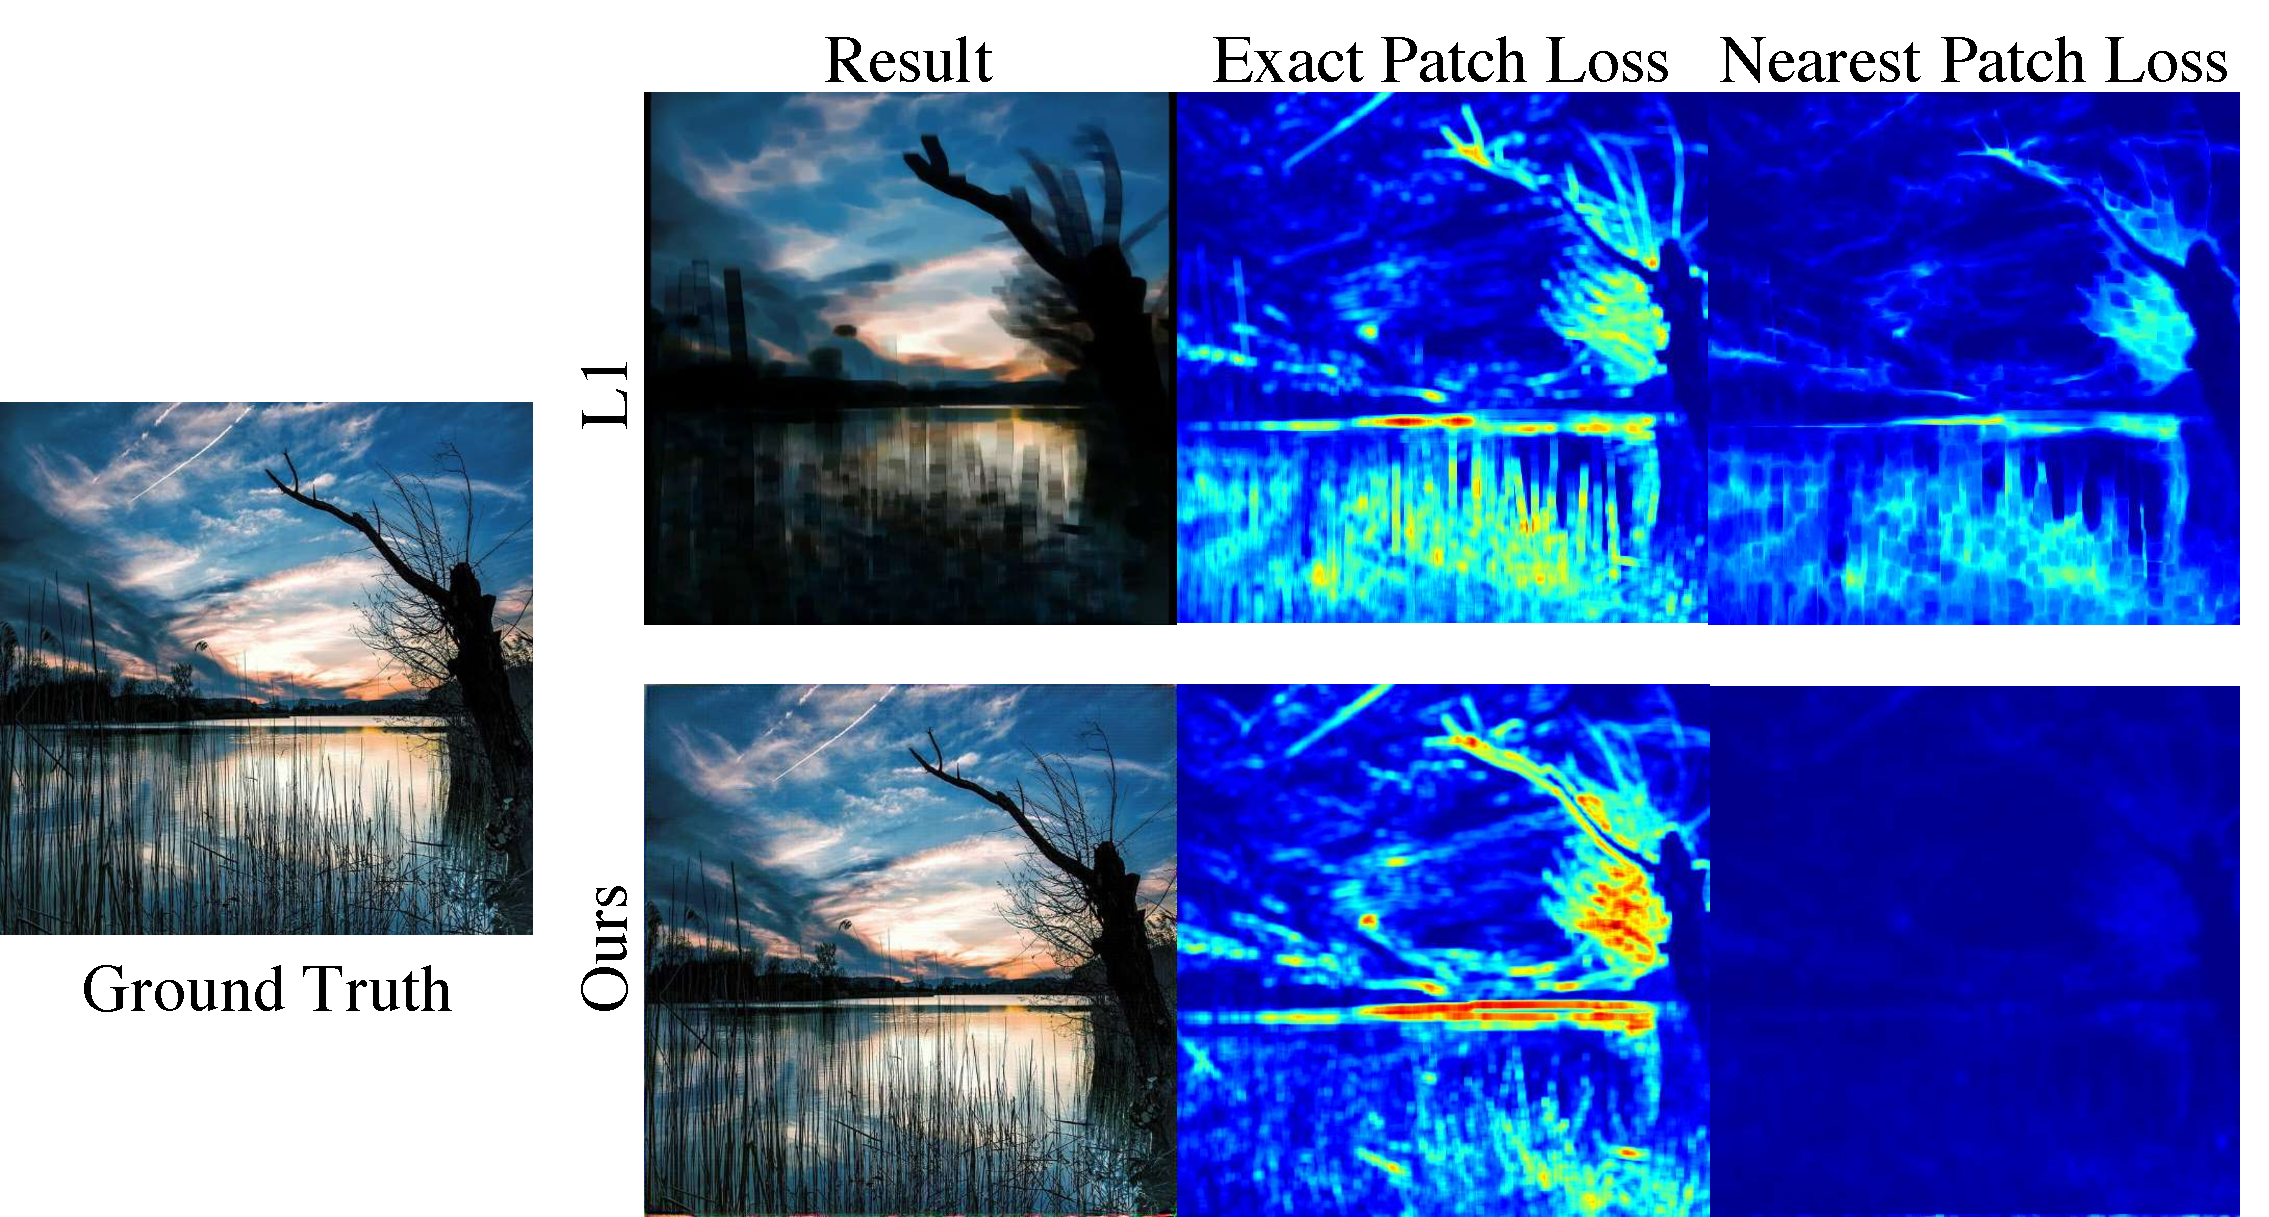
\includegraphics[width=0.8\linewidth]{texturegen/figures/exp2d.pdf}
    \caption{Texture Generation on 2D. The texture provided by our approach is visually closer to the ground truth image while avoiding blurring artifacts such as those introduced by an L1 loss.
    An exact patch loss favors alignment over perceptual similarity, while the nearest patch loss is a more robust metric.
    %Evaluated by exact patch loss, optimization based on L1 loss achieves 10.7 while ours is 11.3. Evaluated by nearest patch loss, L1 achieves 7.33 while ours is 1.53.
    }
    \label{fig:3dlite-2d-example}
\end{figure}

Visually, our optimized image is sharper and perceptually closer to the ground truth while an  L1 loss results in blurry effect from aggregating multiple misaligned observations. 
In this simple setting, we evaluate the exact patch loss for each pixel quantitatively as the L2 distance of patches centered at this pixel between the generated image and the same one in the ground truth. The exact overall exact patch loss is the L2 norm of exact patch losses for all pixels. We additionally evaluate the nearest patch loss.
Optimization with the L1 loss achieves 10.7 exact patch loss while ours is 11.3. However, we achieve 1.53 nearest patch loss, which is smaller than L1 as 7.33. This suggests that our method prefers realistic misalignment to blur. We successfully derive an image where every local patch is nearly identical to a misaligned version of the patch in the ground truth image.

\paragraph*{Synthetic 3D Example}
%\paragraph*{Robust to Camera or Geometry Errors?}
In order to quantitatively evaluate our 3D texture generation, we create a synthetic dataset of 16 models randomly selected from ShapeNet~\cite{chang2015shapenet} across different categories. 
These shapes typically contain sharp edges and self-occlusion boundaries, complexities reflecting those of real-world objects.
Since we aim to address arbitrary texturing, we enrich the appearance of these shapes by using 16 random color images from the internet as texture images. 
To create  virtual scans of the objects, we uniformly sample $>900$ views on a unit hemisphere by subdividing an icosahedron, from which we render the textured geometry as observed color images. 
To simulate misalignment, we associate each rendered image with a slightly perturbed camera pose, and to simulate geometry errors, we apply random perturbations to the geometric model.
We use a set of errors increasing from $n=1$ to $n=4.5$, and refer to the supplemental material for additional detail regarding generating camera and geometry perturbations.


In Table~\ref{tab:toptim-cam-err}, we study the effect of varying camera and geometry errors in this synthetic 3D setting.  We report evaluation metrics for our approach as well as several state-of-the-art texture optimization methods, including methods based on an L1 loss and texturing using sharpest frame selection~\cite{vu2011bf}.
Our approach outperforms all other methods, as it avoids blurring effects often seen with L1 and ColorMap~\cite{zhou2014color}, and it avoids seams and over-sharpness introduced by methods relying on sharpness selection (3DLite~\cite{huang20173dlite} and sharpest frame selection).
VGG~\cite{johnson2016perceptual} aggregates views by blending deep features, which is insufficient for handling misalignment artifacts.
Two example scenes with increasing errors in camera and geometry are shown in Figure~\ref{fig:toptim-pose-visual}.

\begin{table}
    \centering
    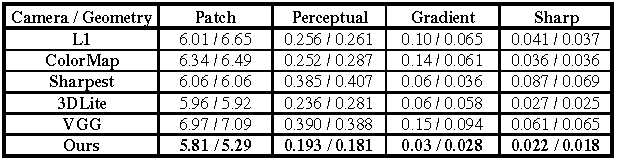
\includegraphics[width=0.8\linewidth]{texturegen/figures/synthetic-table.pdf}
    \caption{Evaluation of different methods on our 3D synthetic dataset averaged across different levels of camera pose and geometry errors.}
    \label{tab:toptim-cam-err}
\end{table}
\begin{figure}
\begin{minipage}{0.49\linewidth}
    \centering
    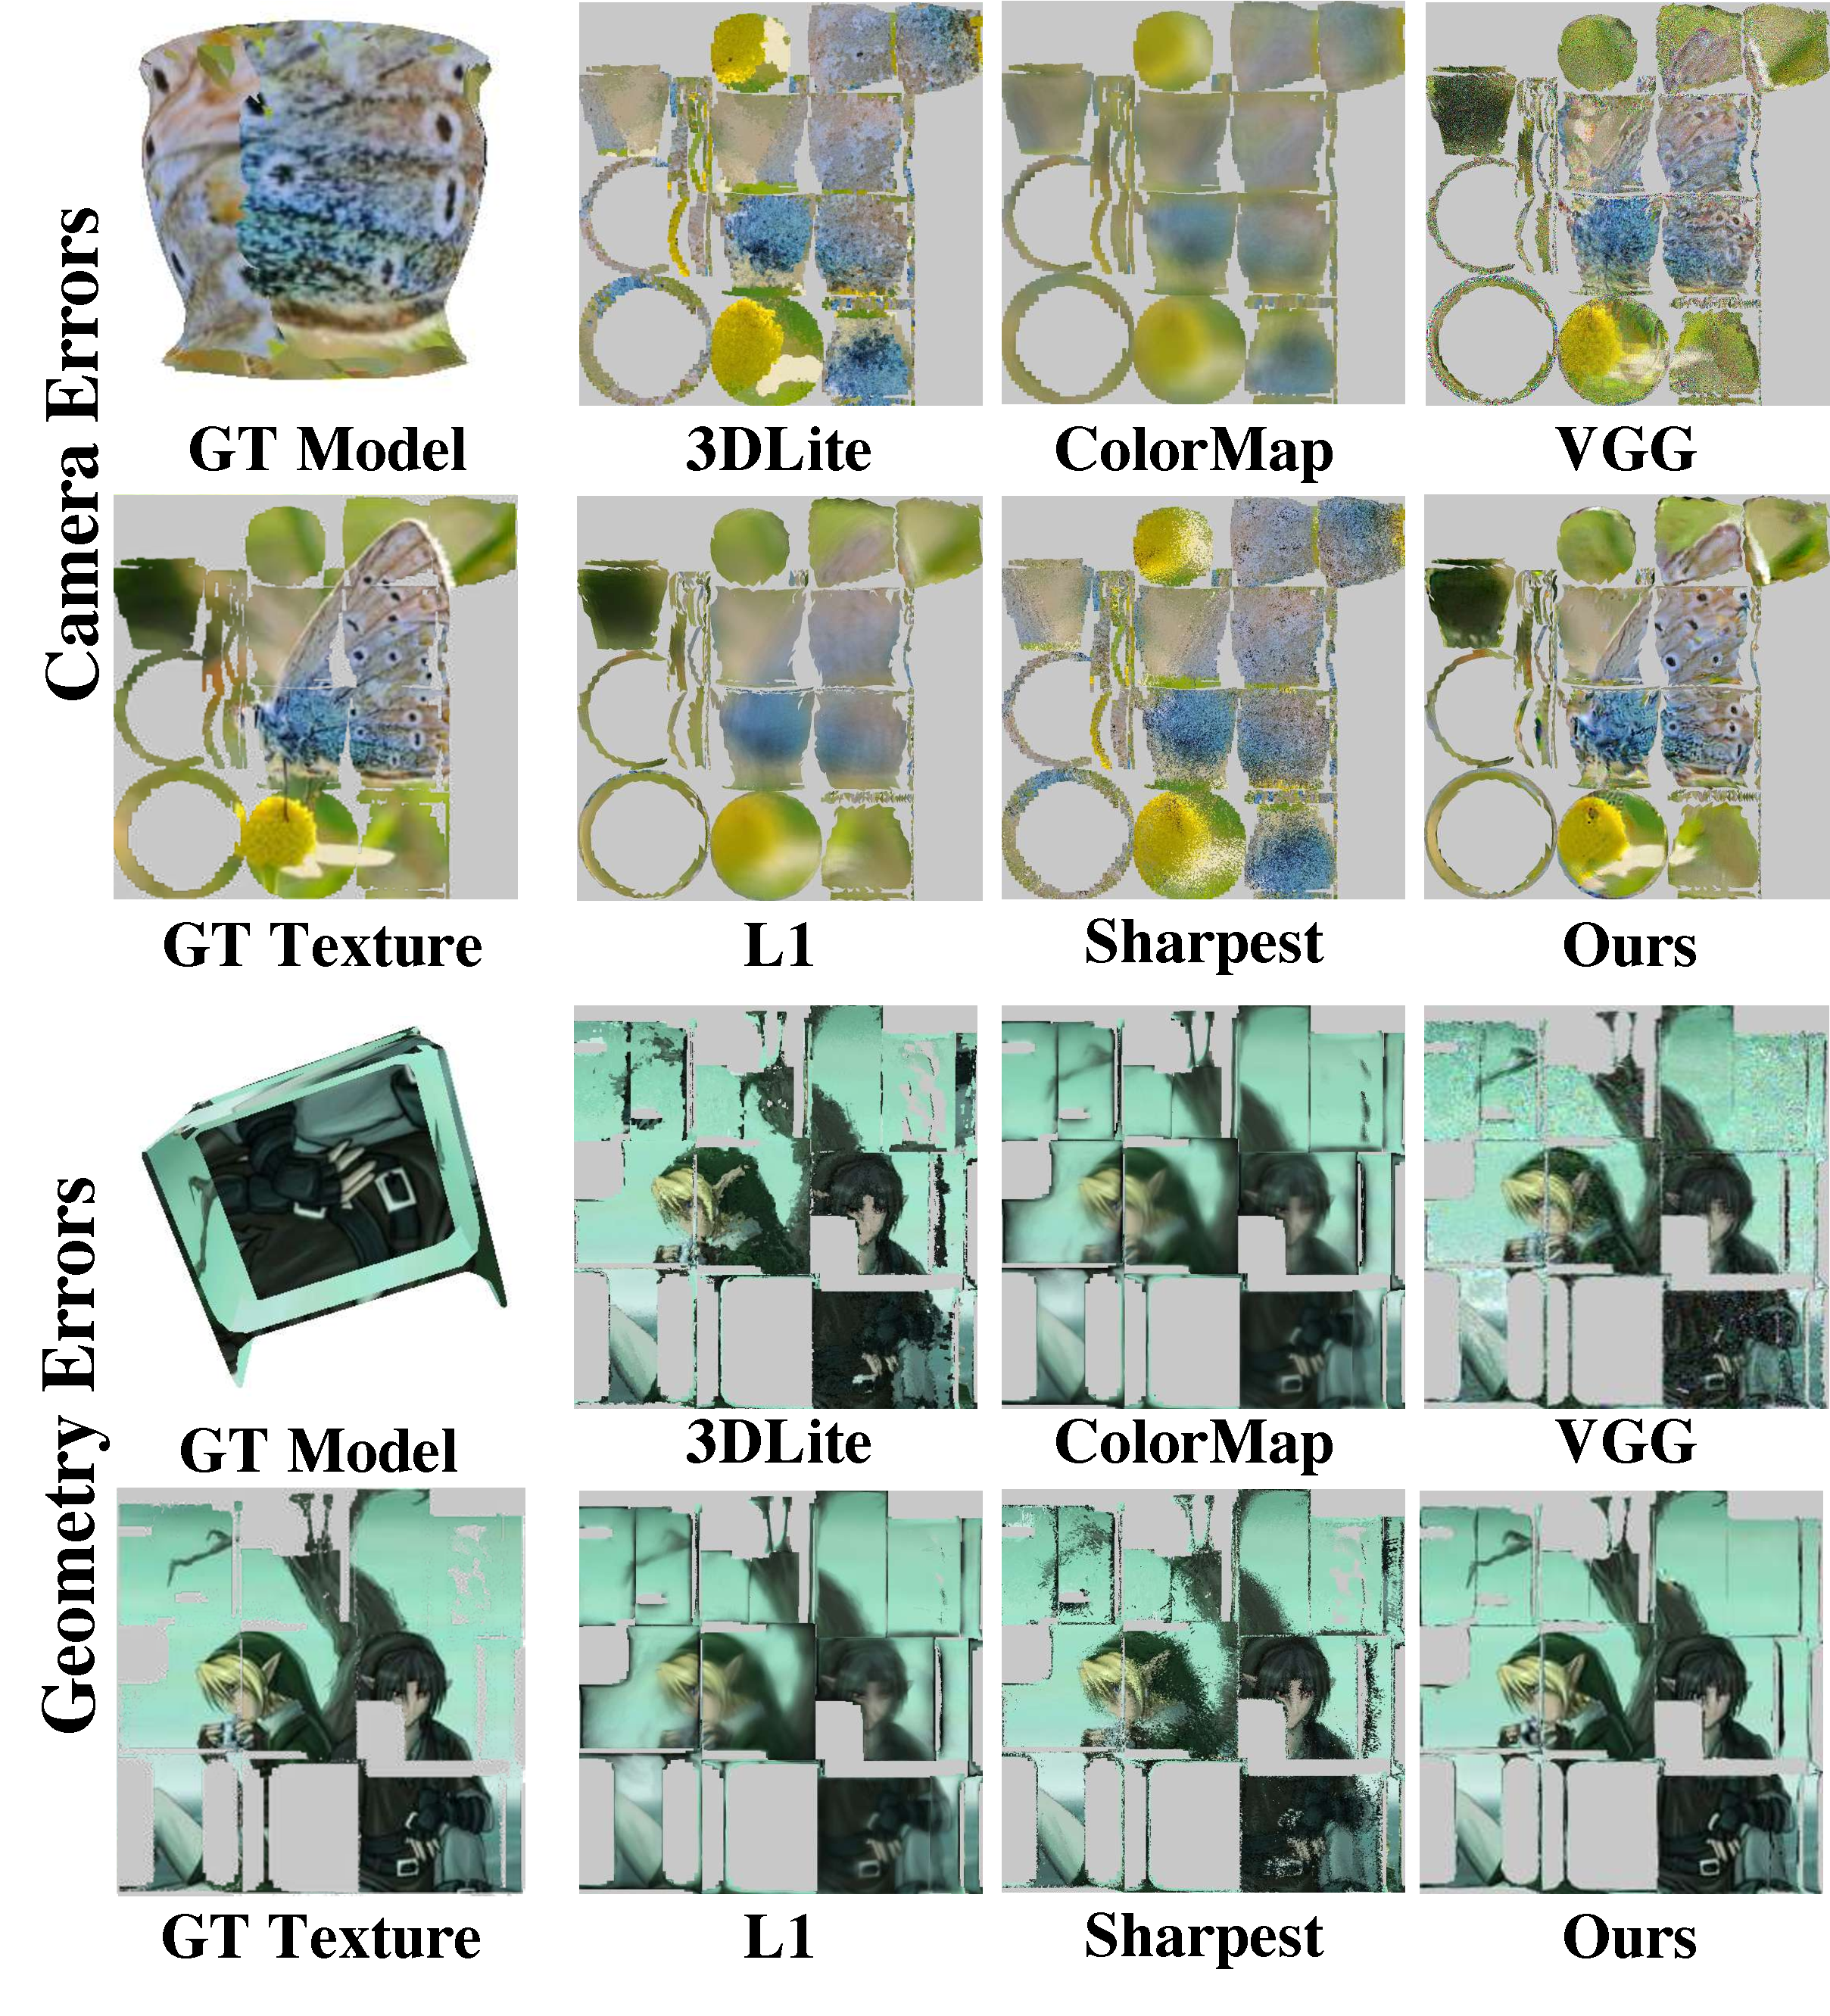
\includegraphics[width=\linewidth]{texturegen/figures/synth-results.pdf}
    \caption{Texture generation in case of high camera or geometry errors. ColorMap~\cite{zhou2014color} cannot handle such large errors. Sharpest or 3DLite~\cite{huang20173dlite} selection leads to inconsistent boundaries or breaks structures. VGG~\cite{johnson2016perceptual} aggregates views by blending deep features with noises, which is not sufficient for handling misalignment artifacts. Ours is visually closest to the ground truth.}
    \label{fig:toptim-pose-visual}
\end{minipage}
\begin{minipage}{0.49\linewidth}
\begin{minipage}{\linewidth}
    \centering
    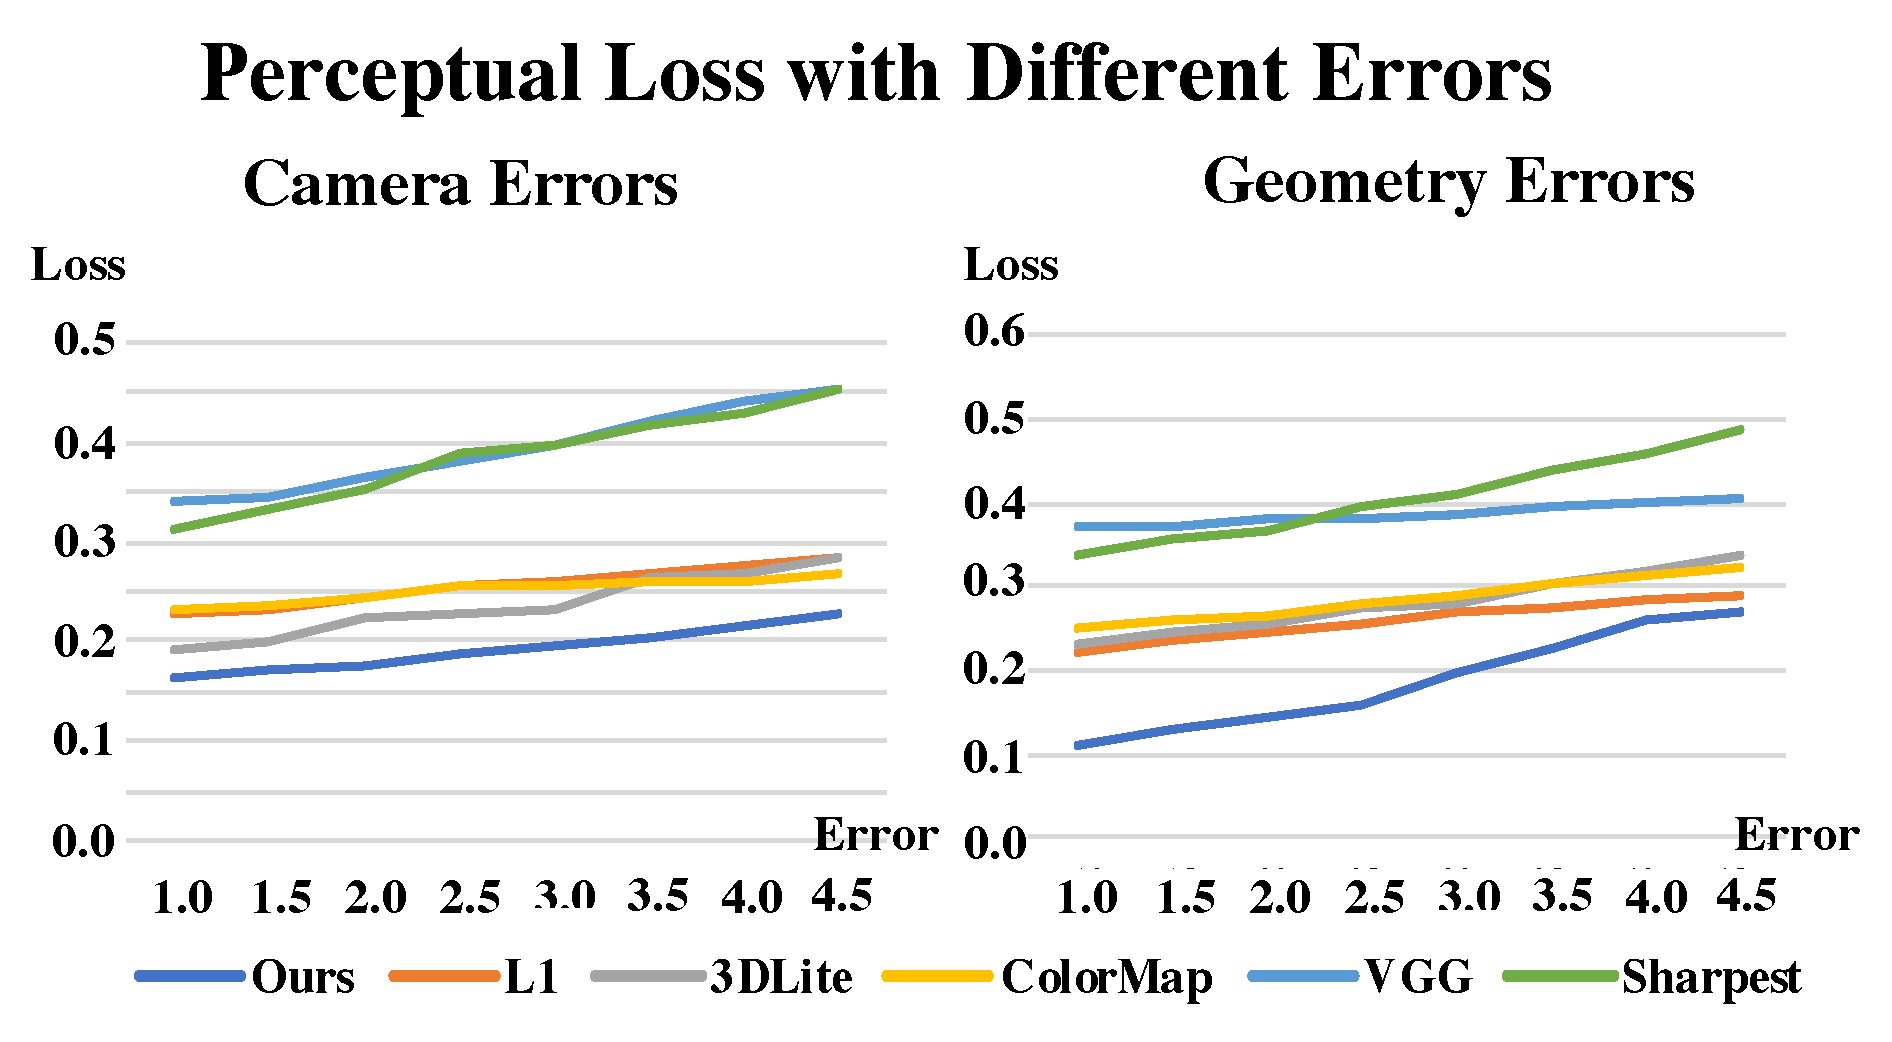
\includegraphics[width=0.9\linewidth]{texturegen/figures/chart.pdf}
    \caption{Perceptual loss of different approaches under increasing camera or geometry errors. Ours outperforms existing methods in different levels of errors.}
    \label{fig:toptim-pose-chart}
\end{minipage}
\begin{minipage}{\linewidth}
    \centering
    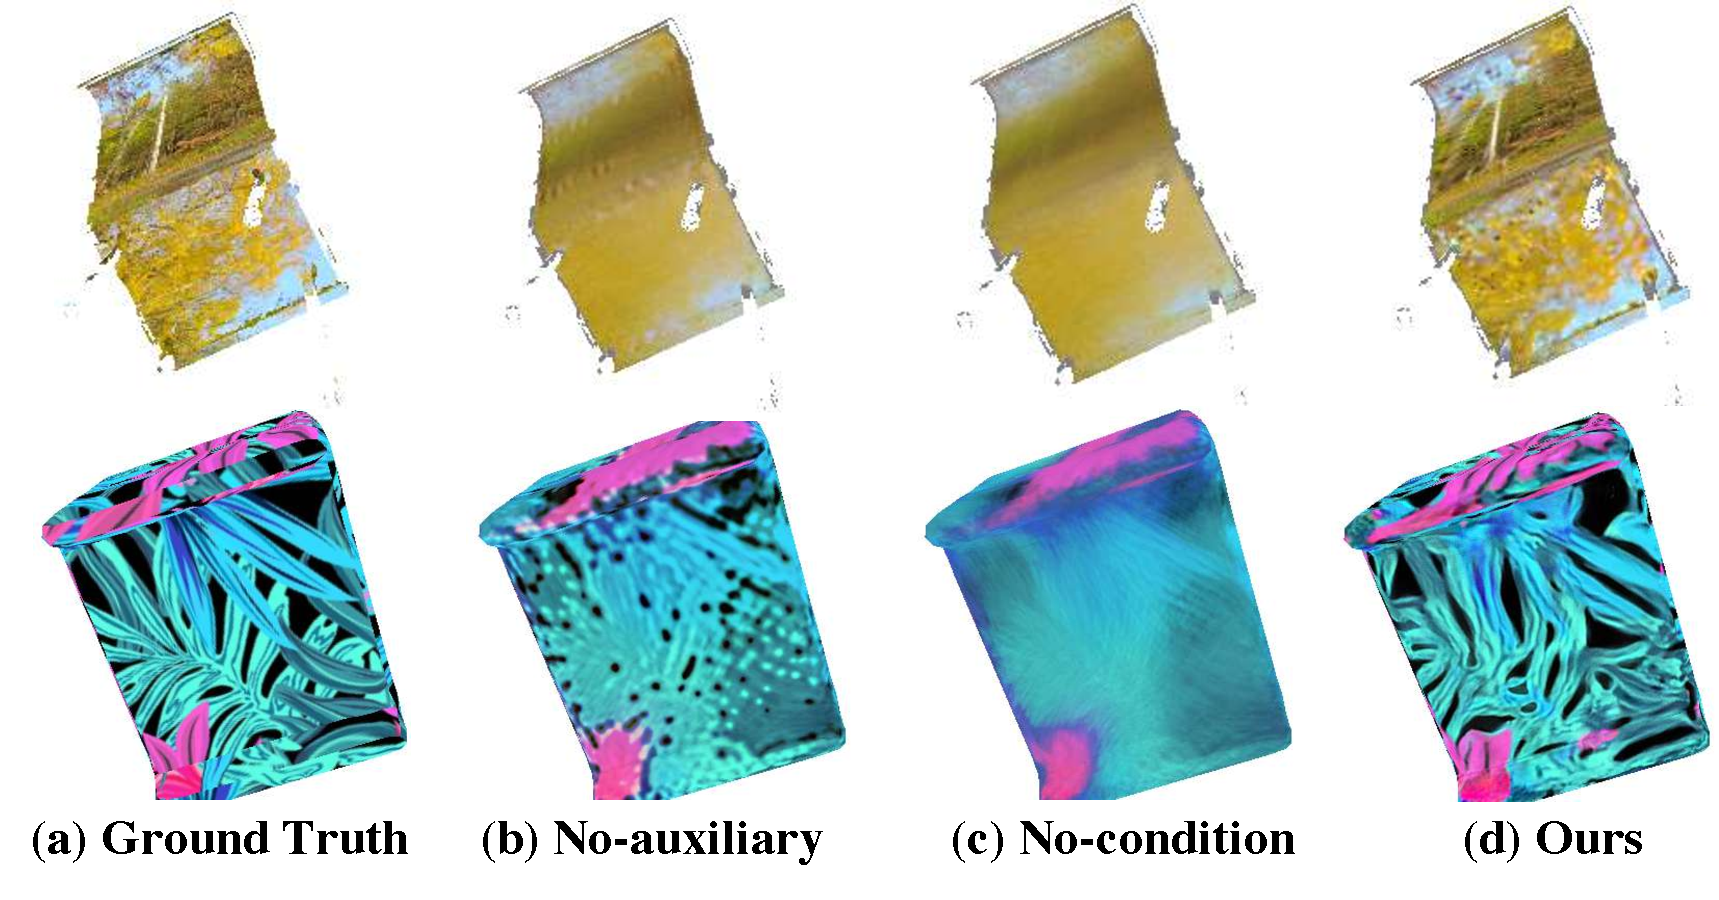
\includegraphics[width=\linewidth]{texturegen/figures/adversarial-compare.pdf}
    \caption{Comparing different discriminator options. (b) removes the auxiliary view from the discriminator, resulting in the lack of robustness to misalignments. (c) removes the condition from the discriminator, resulting in ambiguity in local regions. (d) our conditional discriminator leveraging auxiliary views to provide examples of realistic misalignments enables tolerance to misalignment and generation of textures reflecting input image characteristics. }
    \label{fig:toptim-gan-err}
\end{minipage}
\end{minipage}
\end{figure}

We additionally study the behavior of all methods in this experiment using the perceptual metric~\cite{zhang2018unreasonable} in Figure~\ref{fig:toptim-pose-chart}.
Although the performance drops for all methods with the increase of camera/geometry errors, our approach maintains the best perceptual quality as the errors increase. Visualization of several textured models generated by ColorMap~\cite{zhou2014color} and ours are shown in Figure~\ref{fig:toptim-pose-chart}; our approach maintains a sharp result while ColorMap produces increasingly blurriness as the error increases. 

\begin{figure}
    \centering
    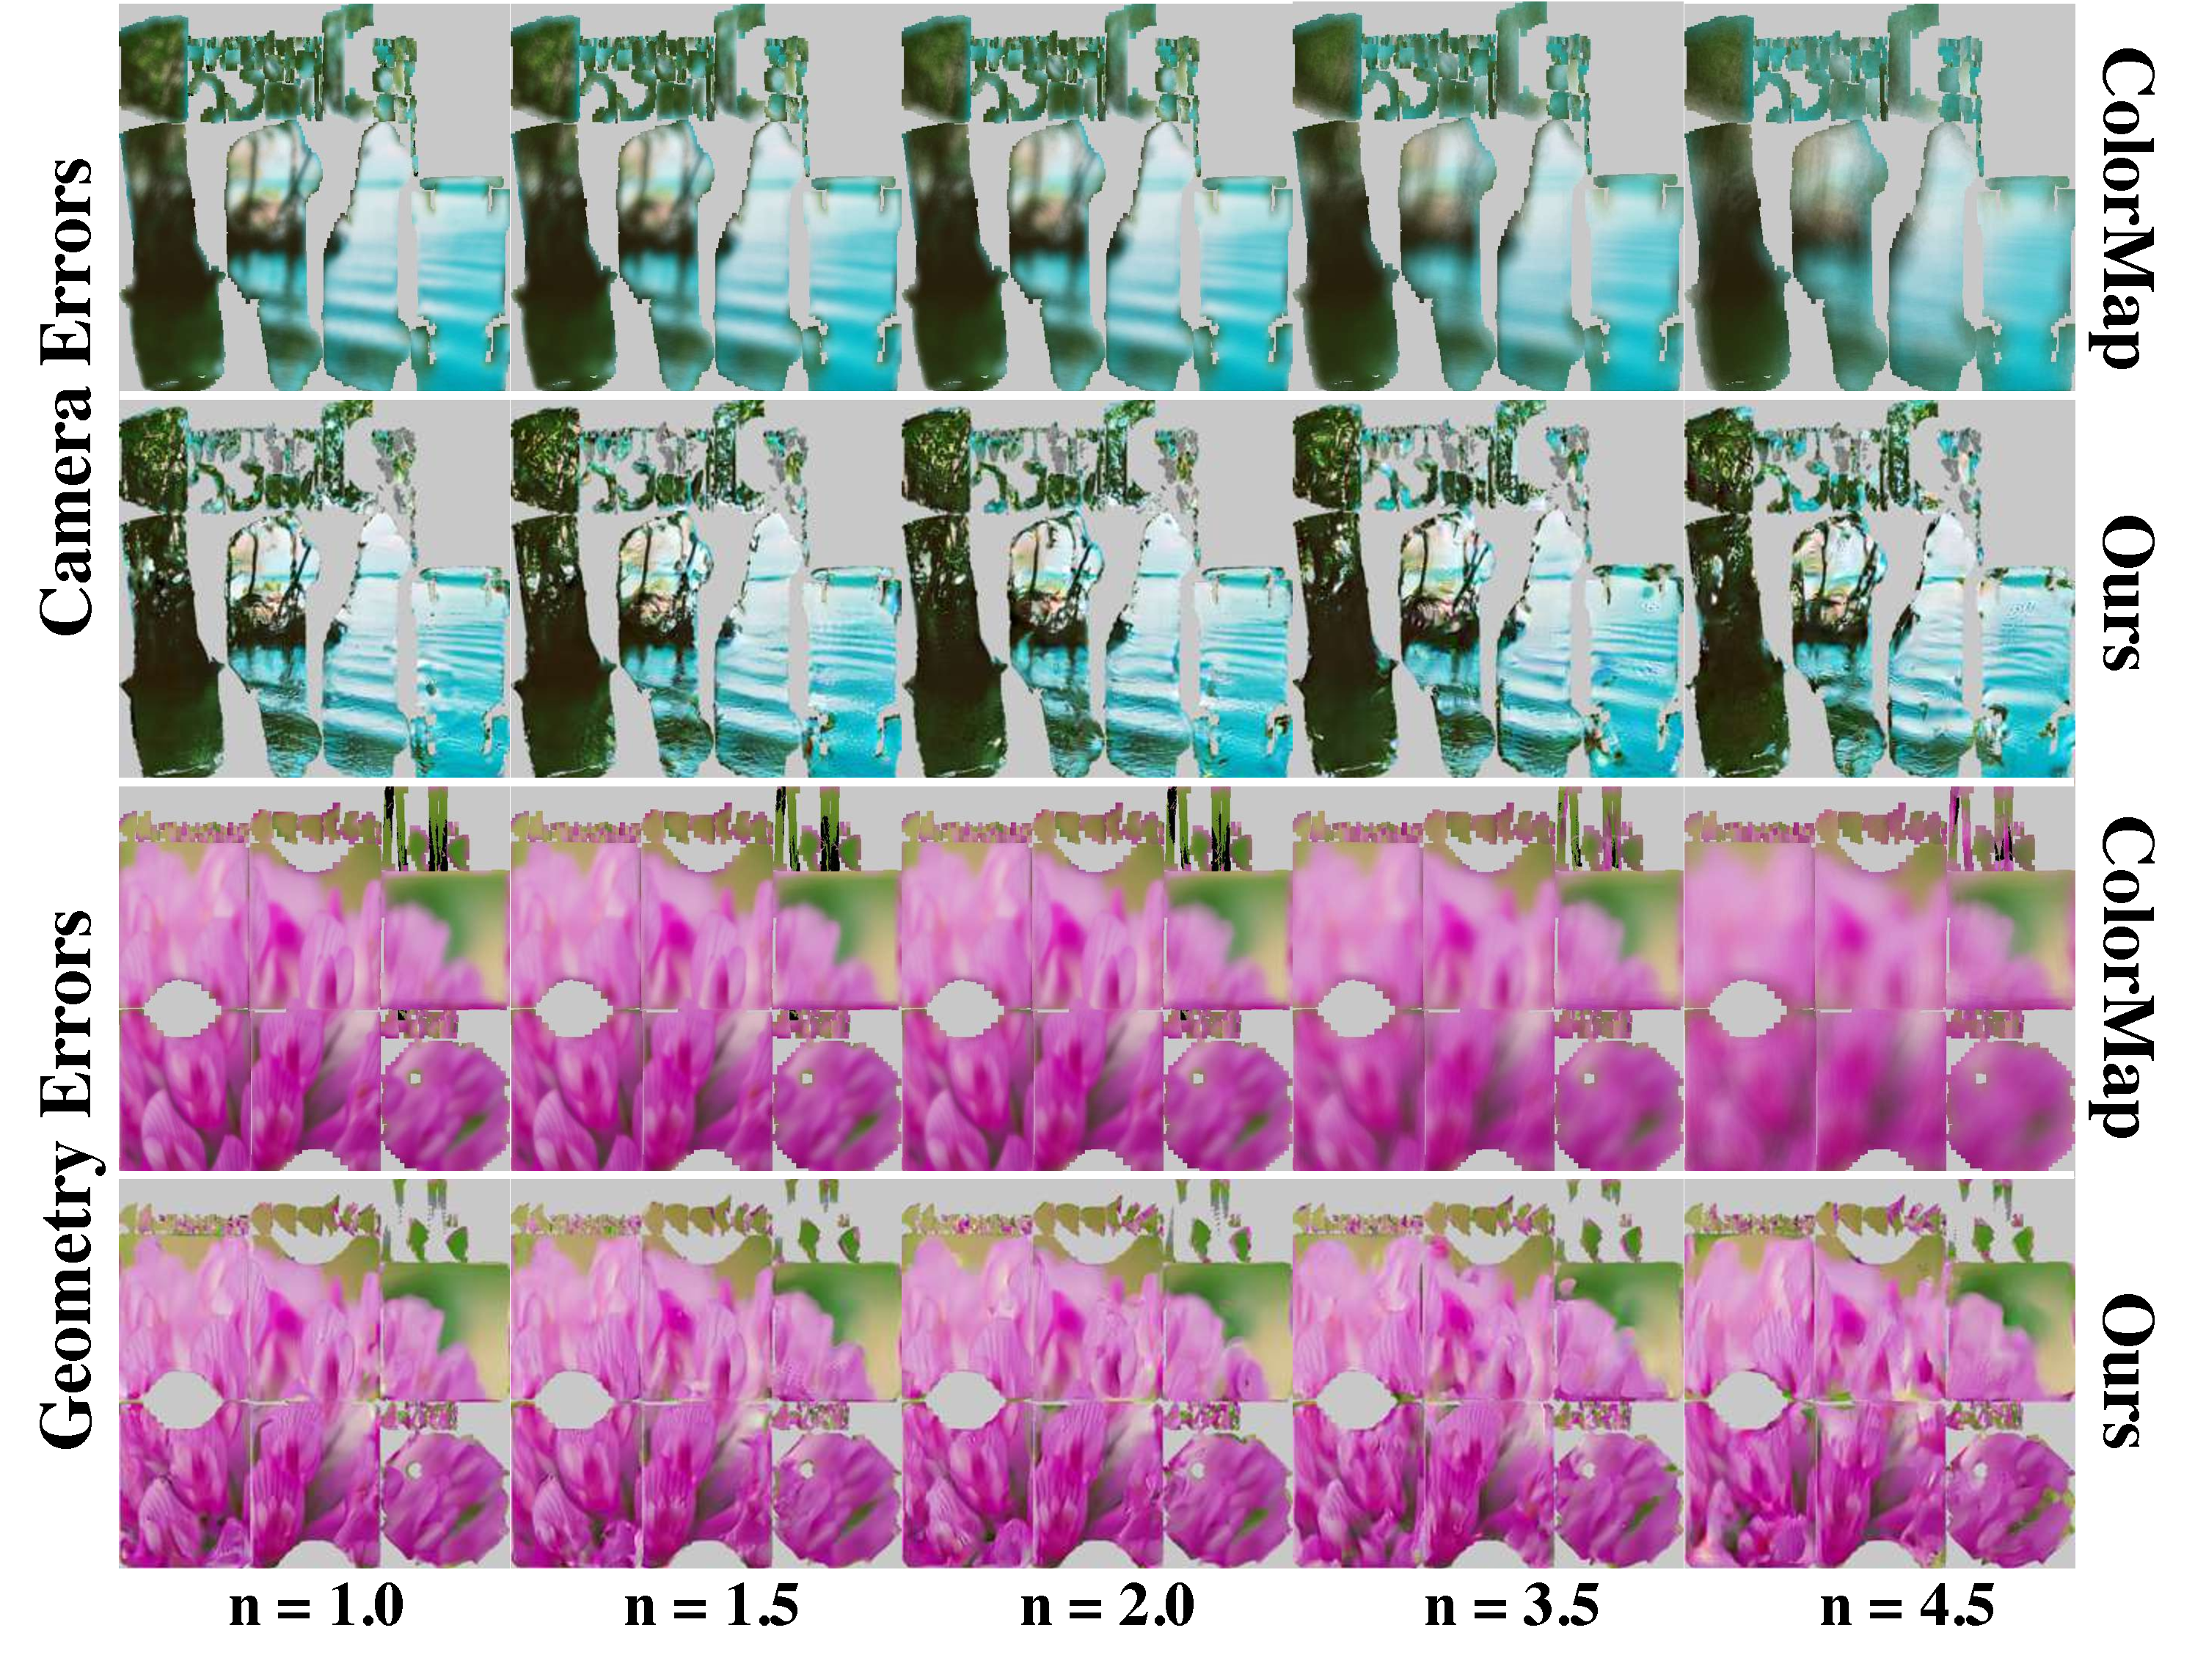
\includegraphics[width=0.8\linewidth]{texturegen/figures/results-synth-diff.pdf}
    \caption{Visualization of texture generation under increasing camera or geometry errors. Under the increase of camera pose/geometry errors, ColorMap~\cite{zhou2014color} produces more blurry results while ours maintains sharp textures.}
    \label{fig:pose-diff}
\end{figure}

\paragraph*{Alternative Choices for Discriminators?} 
We analyze the design choices for our misalignment-tolerant conditional discriminator in Figure~\ref{fig:toptim-gan-err}.
Removing the auxiliary view (b) and thus relying only on the source view to provide `real' examples to the discriminator (similar to pix2pix~\cite{isola2017image}) renders the metric unable to handle misalignments.
We also evaluate a  general discriminator that classifies whether a generated patch is real or fake among entire input view sets without any condition (c), resulting in ambiguity regarding where real patches come from. 
Our conditional discriminator leveraging reprojected auxiliary views enables robustness to misalignment, resulting in realistic texturing.

\paragraph*{Real Object Scans}
We compare our method to state-of-the-art texturing methods on scanned objects from real environments. We use a structure sensor\footnote{https://structure.io} along with its SLAM system to scan 35 chairs, producing scanned geometry, RGB-D frames and the camera poses ($\approx 500$ frames per scan). 
The foreground/background for the object in the RGB frames is determined by whether a ray intersects with the reconstructed geometry. Figure~\ref{fig:toptim-object-scan} (rows 1-4) shows qualitative comparisons.
With an L1 loss or ColorMap~\cite{zhou2014color}, blur artifacts are induced by misalignment errors.
Sharpest selection and 3DLite~\cite{huang20173dlite} use sharp region selection, resulting in seams and inconsistent global structures, as shown in the flower, leaf, and chair arms. 
A VGG loss~\cite{johnson2016perceptual} produces excess noise artifacts.  
Our approach produces sharp and consistent texturing, including detailed patterns such as the leaves in row 1 and woven structures in rows 2 and 3.

Additionally, we show a quantitative evaluation in Table~\ref{tab:toptim-result} (first column) by evaluating the perceptual metric~\cite{zhang2018unreasonable} for rendered textures against input observed views; our approach achieves the most realistic texturing.

\paragraph*{Real Scene Scans}
To demonstrate the capability of our approach to optimize texture on a larger scale, we run our algorithm on the ScanNet dataset~\cite{dai2017scannet}, which provides RGB-D sequences and reconstructed geometry of indoor scenes.
We evaluate our approach on scenes with ID $\leq 20$ ($\approx 2000-3000$ frames per scan) and compare it with the existing state of the arts. 
Figure~\ref{fig:toptim-object-scan} (rows 5-9) and Table~\ref{tab:toptim-result} (middle column) show qualitative and quantitative comparisons. 
Our method produces texturing most perceptually similar to the observed images; our misalignment-tolerant metrics aids in avoiding blur, increased sharpness, or excess noise produces by other methods due to camera and geometry errors in real-world scans.
%We achieve better visual result compared to all other approaches with sharper or more consistent textures. Figure~\ref{fig:toptim-object-scan} (row 5-9) shows a visual comparison among different methods, where our result looks closest to the ground truth images.

\paragraph*{Real to CAD Models}
Since our method can better handle errors due to approximate surface geometry, it is possible to consider texturing CAD models using real-world images to attain realistic appearances.   While large datasets of 3D CAD models are now available~\cite{chang2015shapenet}, they are often untextured or textured simplistically, resulting in notably different appearance from real-world objects. 
To test whether our method can be applied in this challenging scenario, 
%We thus apply our approach to texturing CAD models using real-world imagery, to provide more realistic appearance despite both differing geometry of synthetic CAD models and real-world objects as well as camera errors in captured imagery. To this end, 
we use our collected dataset of real object scans, retrieve similar CAD models from ShapeNet~\cite{chang2015shapenet}, and rigidly align them to the scanned objects.
We then replace the scanned geometry with the CAD model geometry and then use the captured color images and estimated poses from the scan to optimize the CAD texture.
Qualitative and quantitative evaluation of our approach in comparison to existing state-of-the-art methods are show in Figure~\ref{fig:toptim-object-scan} (rows 10-13) and Table~\ref{tab:toptim-result} (right column), respectively.
Our approach is able to handle both camera poses errors as well as the synthetic-real geometry differences to produce texturing perceptually very similar to observed imagery, whereas other methods suffer strong blur, noise, and seam artifacts under these errors.
%, it opens the potential for attaching real world appearance to the CAD models. We manually find the chairs as CAD models in ShapeNet which looks similar to the scanned model and apply a rigid 3D transformation to roughly align them. Then, we replace the scanned geometry with the CAD model and aim at mapping the color information from the scanning video to it. Figure~\ref{fig:toptim-object-scan} (row 10-13) shows the results from different approaches on painting CAD models. Our approach produces minimum artifacts and faithfully paint textures on top of the CAD models.

\paragraph*{Evaluation}
\begin{figure}
\begin{minipage}{0.49\linewidth}
    \centering
    \begin{tabular}{|c|c|c|c|}
        \hline
        & Object & ScanNet & CAD\\
        \hline
        L1 & 0.197 & 0.470 & 0.199 \\
        \hline
        ColorMap & 0.186 & 0.461 & 0.234 \\
        \hline
        Sharpest & 0.222 & 0.510 & 0.260 \\
        \hline
        3DLite & 0.185 & 0.445 & 0.238 \\
        \hline
        VGG & 0.272 & 0.534 & 0.289 \\
        \hline
        Ours & \textbf{0.175} & \textbf{0.395} & \textbf{0.176} \\
        \hline
    \end{tabular}
    \captionof{table}{Mean perceptual loss comparing the input images and rendered textures from different methods. Our method achieves best performance in the real and CAD datasets.}
    \label{tab:toptim-result}
\end{minipage}
\begin{minipage}{0.49\linewidth}
    \centering
    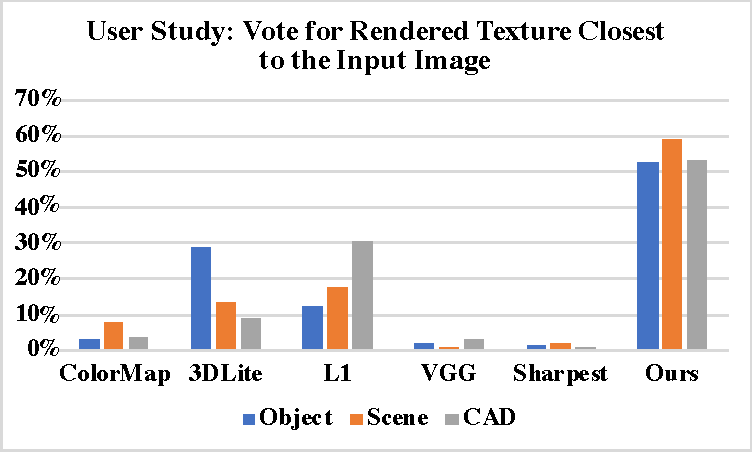
\includegraphics[width=0.8\linewidth]{texturegen/figures/user.pdf}
    \caption{User study. We ask people to vote for the rendered textures from different methods that look closest to the input image.}
    \label{fig:user-study}
\end{minipage}
\end{figure}
Although we lack ground truth texturing for the objects in the real environments, we can compare the perceptual loss~\cite{zhang2018unreasonable} with the rendering of textured geometry at the corresponding viewpoint. We select 10 views uniformly distributed from the scanning video, render the textured model to compute the mean of the perceptual loss.
Table~\ref{tab:toptim-result} shows the performance of different methods on the object scans, scene scans and the CAD models, and our method achieves the best performance in these three scenarios.

Additionally, we perform a user study to evaluate the quality of the texture, shown in Figure~\ref{fig:user-study}.
Our user study comprised $63$ participants who were asked to vote for the texture which produced a rendering closest to the input image. 
For some views, it can sometimes be difficult for users to differentiate between different methods when regions are largely uniform in color. 
Nevertheless, our method is  still notably preferred over other texturing approaches.
\begin{figure}
    \centering
    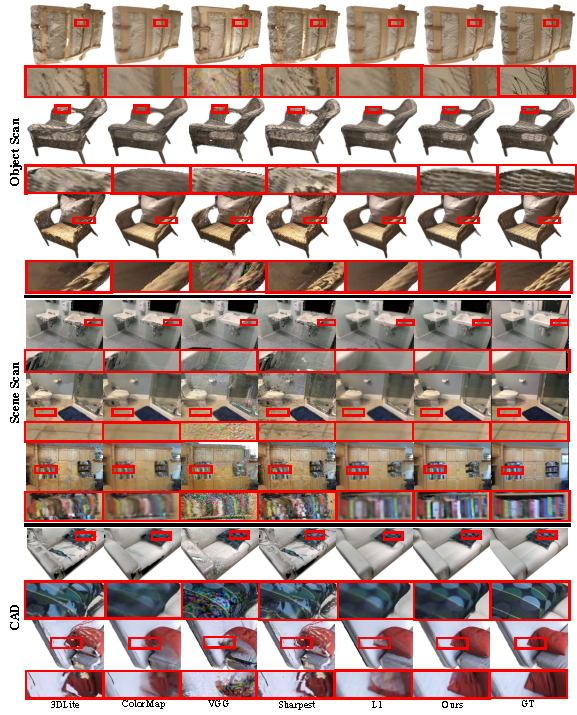
\includegraphics[width=\linewidth,height=1.15\linewidth]{texturegen/figures/result.pdf}
    \caption{Visual comparison on object scans, ScanNet~\cite{dai2017scannet} scans of scenes, and CAD models aligned with object scans. Due to misalignment errors in both camera pose and geometry, both L1 loss and ColorMap~\cite{zhou2014color} produce blurry artifacts, sharpest selection and 3DLite~\cite{huang20173dlite} result in inconsistent regions or breaks in texture structure, and VGG~\cite{johnson2016perceptual} blends learned features resulting in structural artifacts and noise. Our misalignment-tolerant approach produces sharp and consistent textures.}
    \label{fig:toptim-object-scan}
\end{figure}

\chapter{Surface Parameterization}
\label{chapter:param}
In this chapter, we discuss Quadriflow\footnote{This chapter is mainly based on our work in~\cite{huang2018quadriflow}} as a scalable and robust method for quadrangulation, served as a data representation for seamless surface parameterization. We discuss the approach in section~\ref{sec:quad-method}, and evaluate our method in section~\ref{sec:quad-evaluate}.

\section{Methods}
\label{sec:quad-method}
\begin{table}
\centering
\caption{Notation.}
\label{tab:quad-notation}
\begin{tabular}{|l|l|l|l|}
\hline
$\mathcal{M}$ & triangle mesh &
$\mathcal{V}$ & vertices in $\mathcal{M}$\\
\hline
$\mathcal{E}$ & directed edges in $\mathcal{M}$ &
$\mathfrak{E}$ & redirected edges in $\mathcal{M}$\\
\hline
$\mathcal{F}$ & triangles in $\mathcal{M}$ &
$\mathbf{n}_u$ & normal vector at $u$ \\
\hline
$\q_u$ & orientation field at $u$ &
$\mathbf{p}_u$ & position field at $u$\\
\hline
$\rho$ & desired edge length &
$\mathbf{O}_u$ & local frame basis at $u$ \\
\hline
$\mathbf{R}_2(k)$ & \multicolumn{3}{l|}{2D rotation through $90 \cdot k^\circ$}\\
\hline
$\mathbf{R}_3(\mathbf{n},k)$ & \multicolumn{3}{l|}{3D rotation around axis $\mathbf{n}$ through $90 \cdot k^\circ$}\\
\hline
$k_{uv},k_{vu}$ & \multicolumn{3}{l|}{integer rotations to align $\q_u,\q_v$}\\
\hline
$\mathbf{t}_{uv},\mathbf{t}_{vu}$ & \multicolumn{3}{l|}{integer offsets to pull $\mathbf{p}_u,\mathbf{p}_v$ together}\\
\hline
%$\d^k_{uv}$ & \multicolumn{3}{c|}{integer offset from $\mathbf{p}_u$ to $\mathbf{p}_v$ in $k$'s frame}\\
%\hline
${\d}_{uv},{\d}_{vu}$ & \multicolumn{3}{l|}{integer offsets at redirected edge $(u,v)\in\mathfrak{E}$}\\
\hline
$\mathcal{R}^w_{uv}$ & \multicolumn{3}{l|}{rotation matrix to rotate ${\d}_{uv}$ to the frame of $O_w$} \\
\hline
$G$ & \multicolumn{3}{l|}{ network used in the minimum cost flow problem} \\
\hline
$V$ & vertices in $G$ &
$E$ & edges in $G$ \\
\hline
$c$ & capacity of an edge &
$w$ & cost of an edge \\
\hline
$s$ & source of $G$ &
$t$ & sink of $G$ \\
\hline
\end{tabular}
\end{table}

In this section, we discuss the computation of orientation and position fields and our innovations for removing singularities from the latter. We first review the Instant Meshes algorithm of Jakob et al.~\cite{jakob2015instant}, which we use to initialize the orientation and position fields, in Section~\ref{sec:quad-instantmesh}. We impose constraints on the position field's integer offsets to reduce the number of singularities in Section~\ref{sec:quad-constraints}. We propose algorithms to enforce those constraints in Sections~\ref{sec:quad-maxflow} and~\ref{sec:quad-flip}. We re-optimize the position field in Section~\ref{sec:quad-postoptimize} and extract a quad mesh in Section~\ref{sec:quad-quadextraction}. Table~\ref{tab:quad-notation} summarizes our notation. Figure~\ref{fig:quad-computations} distinguishes our contributions from the parts we borrow from Instant Meshes.

\begin{figure}
\centering
\tikzstyle{myarrow} = [line width = 1mm, draw = gray!20, -triangle 45, postaction={draw, line width = 2mm, shorten >=3mm, -}]
\begin{tikzpicture}[
nn/.style={
  thick,
  draw=black,
  rounded corners=3pt,
  minimum width=0.76\linewidth
},
background/.style={
  inner sep=0.2cm,
  fill=gray!20,
  rounded corners=3pt
},
inner sep=5pt,
node distance=3mm,
]

\node[nn] (a) {
\begin{minipage}{0.85\linewidth}
\centering
Optimize Orientation Field: Equation \eqref{eq:quad-im1} in Section \ref{sec:quad-instantmesh}
\end{minipage}
};
\node[nn] (b) [below=of a] {
\begin{minipage}{0.85\linewidth}
\centering
Optimize Position Field: Equation \eqref{eq:quad-im2} in Section \ref{sec:quad-instantmesh}
\end{minipage}
};
%\node[nn] (c) [below=of b] {
%\begin{minipage}{0.9\linewidth}
%Compute integer offset: \hfill $\d^{*u}_{uv} = \textbf{t}^*_{uv}-%\mathbf{R_2} (k^*_{uv} - k^*_{vu})\textbf{t}_{vu}$.
%\end{minipage}
%};
\node[nn] (d) [below=of b] {
\begin{minipage}{0.85\linewidth}
\centering
Enforce Regularity Constraint by MCF: Section \ref{sec:quad-maxflow}
\end{minipage}
};

\node[nn] (e) [below=of d] {
\begin{minipage}{0.85\linewidth}
\centering
Enforce Consistent Orientation Constraint: Section \ref{sec:quad-flip}

\vspace{5pt}
\centering
\begin{tikzpicture}
\node[draw=black,minimum width=0.4\linewidth, minimum height=15pt, inner sep=0] (G) {Greedy Method};
\node[draw=black,minimum width=0.4\linewidth, minimum height=15pt, inner sep=0] (S) [right=of G] {SAT Reduction};
\end{tikzpicture}
\end{minipage}
};

\node[nn] (f) [below=of e] {
\begin{minipage}{0.85\linewidth}
\centering
Re-optimize Position Field: Equation \eqref{eq:quad-post} in Section \ref{sec:quad-postoptimize}
%\hfill $\p^{\star} = \argmin E_{\mathit{post}}(\p, \d^{\star})$.
\end{minipage}
};

\node[nn] (g) [below=of f] {
\begin{minipage}{0.85\linewidth}
\centering
Quad Mesh Extraction from Position Field: Section \ref{sec:quad-quadextraction}
%\hfill $\p^{\star} = \argmin E_{\mathit{post}}(\p, \d^{\star})$.
\end{minipage}
};

\begin{pgfonlayer}{background}
% \node[background,fit=(a) (b)] (s0) {};
% \node[background,fit=(g)] (s2) {};
\node[background,fit=(d) (e) (f)] (s1) {};
\end{pgfonlayer}

\draw[myarrow] ([xshift = 5mm, yshift=3.4mm]a.east) -- ([xshift = 5mm, yshift=-3.4mm]g.east);

\end{tikzpicture}

\caption{The pipeline of QuadriFlow.  The white nodes are from Instant Meshes~\cite{jakob2015instant}; the shaded nodes are our contribution.}
\label{fig:quad-computations}
\end{figure}


\subsection{Instant Field-Aligned Meshes}
\label{sec:quad-instantmesh}


\begin{figure}
\centering
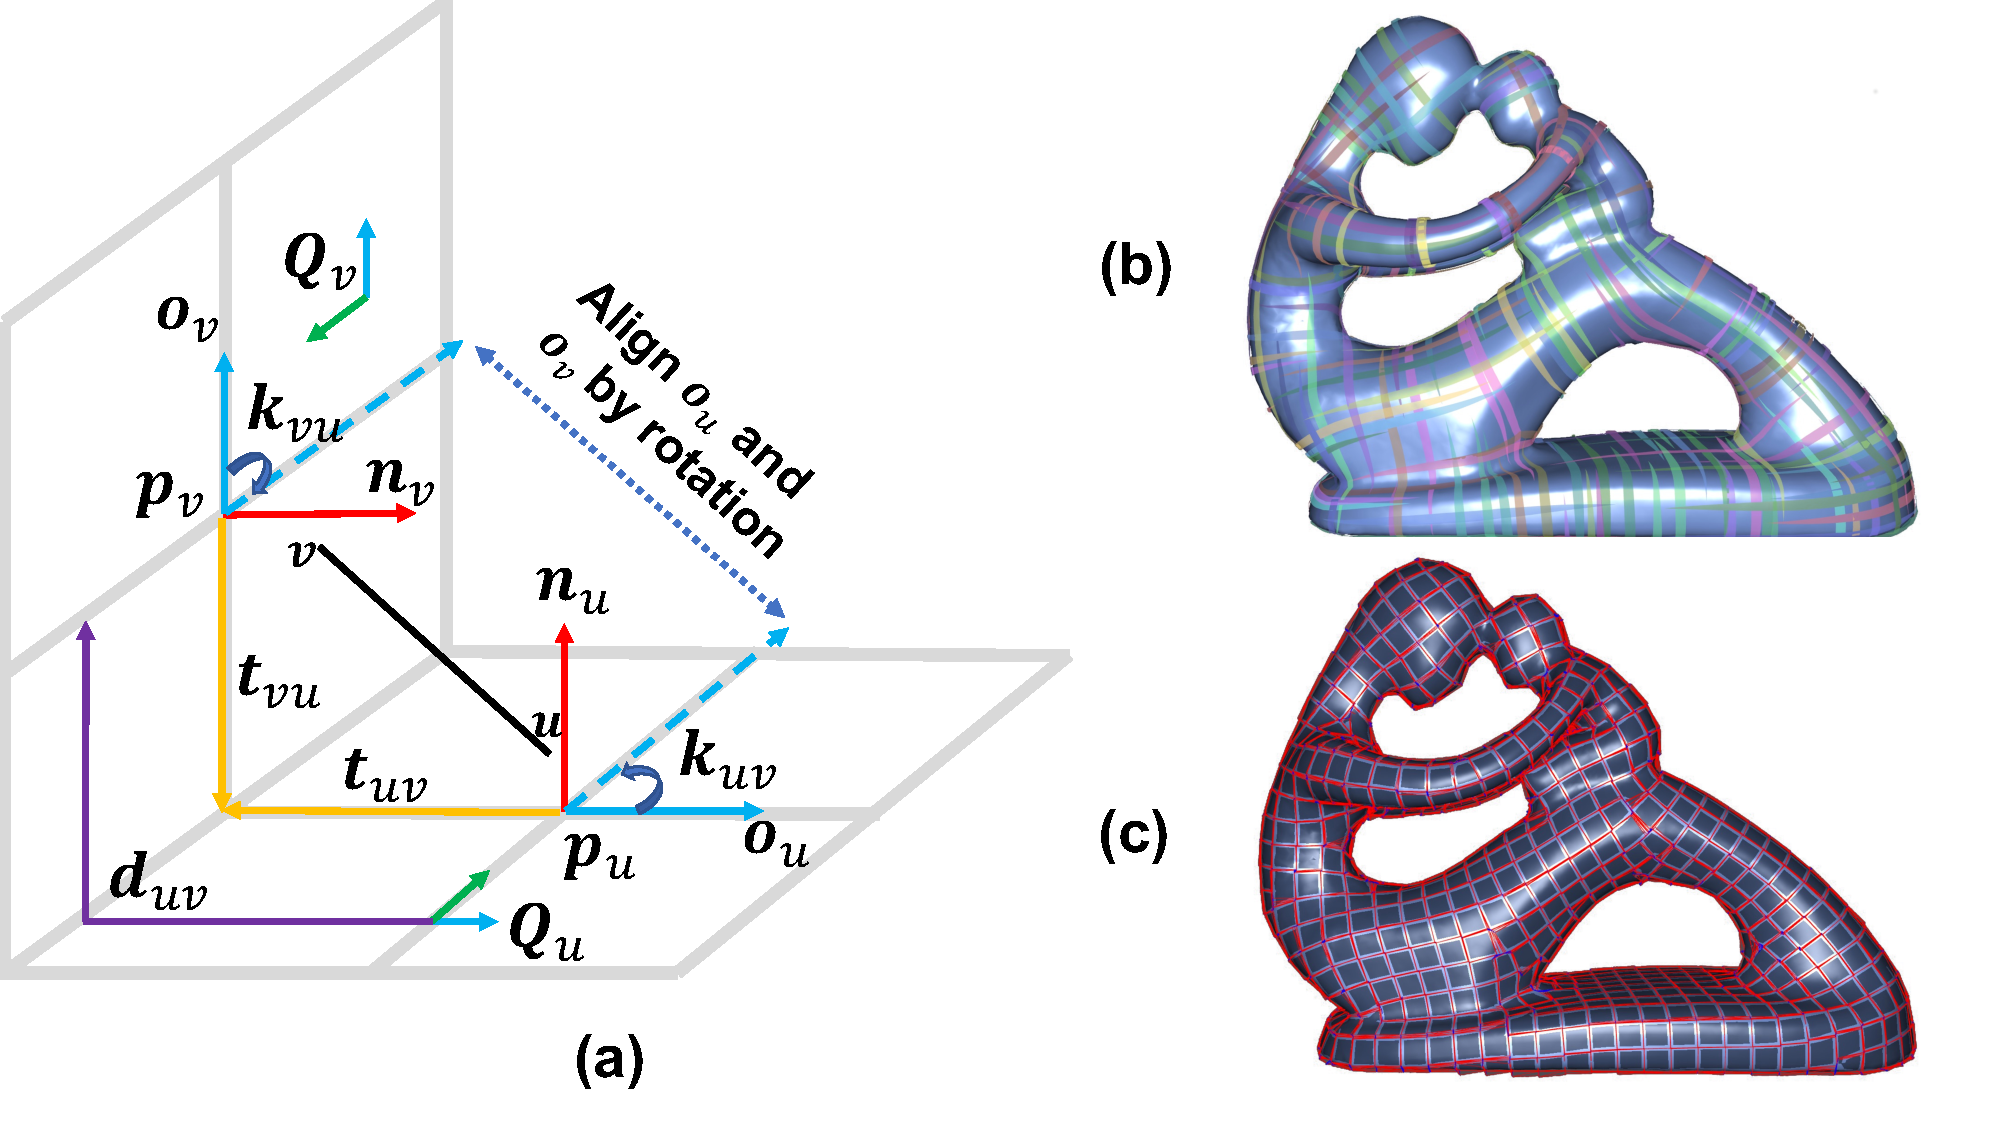
\includegraphics[width=0.6\linewidth]{quadriflow/diagram/instant.pdf}\\
\caption{Geometry (a), orientation field (b), and position field (c), per Jakob et al.~\cite{jakob2015instant}. The adjacent vertices $u$ and $v$ with positions $\mathbf{p}_u$ and $\mathbf{p}_v$ lie on orthogonal tangent planes with normal vectors $\mathbf{n}_u$ and $\mathbf{n}_v$. $\q_u$ and $\q_v$ can be aligned by rotating them through $90 \cdot k_{uv}^\circ$ and $90 \cdot k_{vu}^\circ$. Jakob et al.\ try to make a point on one lattice nearly coincide with a point on the other lattice; these two points are at an integer offset of $\mathbf{t}_{uv}$ lattice points from $\mathbf{p}_u$ and $\mathbf{t}_{vu}$ lattice points from $\mathbf{p}_v$ in local frames. The integer offset $\d_{uv}$ is the sum of these integer translations in $u$'s frame.}
\label{fig:quad-instant}
\end{figure}

Here, we recapitulate the main ideas of Instant Meshes~\cite{jakob2015instant}.  Let $\mathcal{M} = (\mathcal{V}, \mathcal{F}, \mathcal{E})$ be an input surface triangulation where $\mathcal{V} = \{ 1, 2, \ldots, |\mathcal{V}| \}$ is a set of vertex indices, $\mathcal{E} \subseteq \mathcal{V} \times \mathcal{V}$ is a set of directed edges, and $\mathcal{F}$ is a set of triangular faces.

\paragraph*{Orientation Field.}
The first step is to compute a four-way rotationally symmetric (\emph{4-RoSy}) \emph{orientation field} \cite{ray2008n}. 4-RoSy fields are also known as \emph{cross fields}; the orientation field maps each vertex of $\mathcal{M}$ to a cross that is locally tangent to the surface. Each cross is invariant to rotations by $90^\circ$ in its tangent plane. The orientation field guides the alignment of the edges in the quad mesh. For each vertex $v \in \mathcal{V}$, Jakob et al.\ represent the cross at $v$ with a \emph{representative direction} vector $\q_v \in \R^3$ that lies in vertex $v$'s tangent plane; that is, $\q_v$ is orthogonal to $v$'s normal vector $\mathbf{n}_v$. To obtain representational invariance, let $\mathbf{R}_3(\textbf{n}, k) \in \R^{3 \times 3}$ be a 3D rotation matrix that rotates a vector through $90 \cdot k^\circ$ counterclockwise around an axis $\textbf{n}$ (which is the local normal vector). To smooth the orientation field $\q$, Jakob et al.\ define the \emph{extrinsic smoothness \mbox{energy}} of $\q$ to be
\begin{equation*}
E_o(\q, k) = \sum_{(u,v) \in \mathcal{E}}
\measuredangle \Big(\mathbf{R_3} (\textbf{n}_u,k_{uv}) \q_u, \mathbf{R_3} (\textbf{n}_v,k_{vu}) \q_v\Big)^2,
\end{equation*}
where $\measuredangle(\cdot, \cdot)$ denotes the angle between two vectors, $k_{uv}, k_{vu} \in \{0, 1, 2, 3\}$, and $\n_u$ and $\n_v$ are the normal vectors of vertices $u$ and $v$. The integers $k_{uv}$ and $k_{vu}$ are chosen to make the angle as small as possible. Figure~\ref{fig:quad-instant}(a) illustrates how $\q_u$ and $\q_v$ are realigned by $k_{uv}$ and $k_{vu}$ to point in similar directions (in this example, the same direction). Jakob et al.\ show how to use a mixed-integer Gauss--Seidel algorithm to find
\begin{equation}
\q^*,\, k^* = \argmin_{\q, k} E_o(\q, k) \label{eq:quad-im1},
\end{equation}
thereby obtaining a smooth orientation field like the one illustrated in Figure~\ref{fig:quad-instant}(b). With this extrinsic energy, the orientation field $\q^*$ also aligns well with shape features of the input geometry.

\paragraph*{Position Field.}
Given an orientation field $\q^*$, Jakob et al.\ compute a consistent \emph{position field} that determines the placement of the vertices of the quadrilateral mesh. Let $\rho$ be a user-specified distance specifying the desired length of the edges in the output mesh. For each vertex $v \in \mathcal{V}$, the position field maps $v$ to a square lattice that lies in $v$'s tangent space, has all its edge lengths equal to $\rho$, and is aligned with the cross field as indicated by $\q^*_v$. The lattice is invariant under ``horizontal'' or ``vertical'' translations of distance $\rho$---that is, in the directions $\q^*_v$ or $\textbf{n}_v\times\q^*_v$. (Jakob et al.\ call this \emph{positional symmetry} or \emph{PoSy}.) Hence the only degrees of freedom for the lattice can be specified as ``fractional'' horizontal and vertical translations in the range $[0, \rho)$. For a vertex $v \in \mathcal{V}$, let $\p_v \in \R^3$ be a representative lattice point near vertex $v$ in $v$'s tangent plane. Let
\begin{equation*}
\textbf{O}_v =[\q^*_v,\,\textbf{n}_v\times\q^*_v]
\label{eq:frame}
\end{equation*}
be a basis for $v$'s tangent plane whose basis vectors are aligned with the orientation field.
The \emph{tangent lattice} for $v$ is
\begin{eqnarray*}
\mathcal{T}(\textbf{p}_v, \textbf{n}_v, \q^*_v) & = & \{ \mathcal{T}(\textbf{p}_v, \textbf{n}_v, \q^*_v, \textbf{t}): \t \in \mathbb{Z}^2 \}  \mbox{~where}  \\
\mathcal{T}(\textbf{p}_v, \textbf{n}_v, \q^*_v, \textbf{t}) & = & \textbf{p}_v + \rho \textbf{O}_v \textbf{t}.
\end{eqnarray*}

It is desirable for vertices joined by an edge in $\mathcal{E}$ to have tangent lattices that coincide or nearly coincide---or, more realistically, to each have one nearby vertex in its lattice such that the two vertices nearly coincide. Figure~\ref{fig:quad-instant}(a) illustrates the two tangential lattices of vertices $u$ and $v$ represented by $\mathbf{p}_u$ and $\mathbf{p}_v$, whose lattice points happen to coincide on the intersection of the two planes. To smooth the position field $\mathbf{p}$, Jakob et al.\ define the extrinsic smoothness energy  of $\mathbf{p}$ to be
\begin{equation*}
E_p(\p,\textbf{t})=\sum_{(u,v) \in \mathcal{E}} \Big\Vert\mathcal{T}(\textbf{p}_u, \textbf{n}_u, \q^*_u, \textbf{t}_{uv}) - \mathcal{T}(\textbf{p}_v, \textbf{n}_v, \q^*_v, \textbf{t}_{vu}) \Big\Vert_2^2,
\end{equation*}
where $\t_{uv}, \t_{vu} \in \mathbb{Z}^2$ are selected to remove the translation ambiguity and make the distance as small as possible. As with the orientation field, Jakob et al.\ use a mixed-integer Gauss--Seidel algorithm to find the minimizer
\begin{equation}
\p^*,\, \t^* = \argmin_{\p, \t} E_p(\p, \t). \label{eq:quad-im2}
\end{equation}
This smoothing procedure produces a position field $\mathbf{p}^*$ smooth enough to obtain a quad mesh, most of whose edges have length close to (but not exactly) $\rho$, as shown in Figure~\ref{fig:quad-instant}(c).

\subsection{Integer Offsets and Constraints}
\label{sec:intdef}

%By minimizing $E_p$, we obtain optimal position field $P$ and integer offset relationship between each pair of neighboring vertices $i$ and $j$. Ideally, $||\mathcal{T}(\textbf{p}_i,\textbf{n}_i,\textbf{o}_i,\textbf{t}_{ij})-\mathcal{T}(\textbf{p}_j,\textbf{n}_j,\textbf{o}_j,\textbf{t}_{ji})||_2\simeq 0$ and $\measuredangle(\mathcal{R} (\textbf{o}_{i},\textbf{n}_i,k_{ij}), \mathcal{R} (\textbf{o}_{j},\textbf{n}_j,k_{ji}))\simeq 0$, and we can obtain

%\begin{equation*}
%\textbf{p}_j - \textbf{p}_i \simeq \mathcal{T}(\textbf{p}_i,\textbf{n}_i,\textbf{o}_i,\textbf{t}_{ij}-\mathcal{R}_k ( k_{ij} - k_{ji} )\cdot \textbf{t}_{ji})
%\end{equation*}
%where $\mathcal{R}_k (k)$ is a 2-by-2 matrix representing a 2D rotation by $90 \cdot k$ degree. $\textbf{t}_{ij}-\mathcal{R}_k (k_{ij} - k_{ji})\cdot \textbf{t}_{ji})$ can be viewed as the 2D integer offsets from $\textbf{p}_i$ to $\textbf{p}_j$ in $i$-th frame defined by $\textbf{o}_i$ and $\textbf{n}_i\times \textbf{o}_i$.
%We first initialize the orientation field and position field.
\paragraph*{Integer Offsets.}
Jakob et al.\ note that a singularity appears in the position field when the sum of integer offsets over a triangle in the triangle mesh $\mathcal{M}$ is nonzero. To mathematically express this observation, we first define the integer offset along an edge of $\mathcal{M}$. We find it useful to redirect the mesh edges $\mathcal{E}$ in a canonical way, with each edge directed from the vertex with lesser index to the vertex with greater index.
\begin{defn}
Let
\[
\mathfrak{E}:=\{ (u,v): u < v \mathrm{~and~} ( (u,v) \in \mathcal{E} \mathrm{~or~} (v,u) \in \mathcal{E}) \}
\]
be the set of \emph{redirected edges}.  For each redirected edge $e=(u,v) \in \mathfrak{E}$, define the 2D integer offset
\[
\td^*_e= \textbf{t}^*_{uv}-\mathbf{R_2} (k^*_{uv} - k^*_{vu})\textbf{t}^*_{vu},
\]
the integer offset from $u$ to $v$ in $u$'s frame, where $\mathbf{R_2}(k)$ is a 2D rotation matrix through $90 \cdot k^{\circ}$.  For notational convenience, we use $\td_e$, $\td_{uv}$, and $\td_{vu}$ interchangeably in the following paragraphs.
\end{defn}

After we optimize~(\ref{eq:quad-im2}), $\textbf{p}^*_u$ and $\textbf{p}^*_v$ should be close to each other after applying the integer offsets $\textbf{t}^*_{uv}$ and $\textbf{t}^*_{vu}$ in the frames of $\textbf{O}_u$ and $\textbf{O}_v$, respectively. The formula for the offset is based on the observation that $\textbf{t}_{vu}$ in frame $\textbf{O}_v$ can be measured in frame $\textbf{O}_u$ as $\mathbf{R_2}(k_{uv}-k_{vu})\textbf{t}_{vu}$. See the purple vector in Figure~\ref{fig:quad-instant}(a) for an interpretation of ${\d}_{uv}$.

To detect singularities in the position field, we sum up the integer offsets of the three edges of a triangle under a single frame. For any $(u,v)\in\mathcal{E}$ and any $w$ adjacent to both $u$ and $v$ (including $w=u$), the integer offset for an edge $(u,v)$ in the frame of vertex $w$ can be achieved by applying a 2D rotation $\mathcal{R}^w_{uv}$ to $\td_{uv}$. Specifically, if $u<v$, we can directly change the frame from $u$ to $w$ by a rotation along edge $(w,u)$: $\mathcal{R}^w_{uv}=\mathbf{R}_2(k_{wu}-k_{uw})$. For $u>v$, we first compute the translation from $u$ to $v$ in $v$'s frame as $-\td_{uv}$, and apply the rotation along edge $(w,v)$: $\mathcal{R}^w_{uv}=-\mathbf{R}_2(k_{wv}-k_{vw})=\mathbf{R}_2(k_{wv}-k_{vw}+2)$.

\label{sec:quad-constraints}
\paragraph*{Regularity Constraints.}
If the sum of the integer offsets over a triangle element is nonzero, this triangle encloses a singularity in the position field~\cite{jakob2015instant}. Hence we can remove the singularities from the position field if we can enforce
\begin{equation}
\mathcal{R}^u_{uv}\td_{uv} + \mathcal{R}^u_{vw}\td_{vw} + \mathcal{R}^u_{wu}\td_{wu} = 0 \quad \forall \Delta_{uvw}\in \mathcal{F}.
\label{eq:quad-consistent}
\end{equation}

\paragraph*{Consistent Orientation Constraints.}
%\begin{figure}
%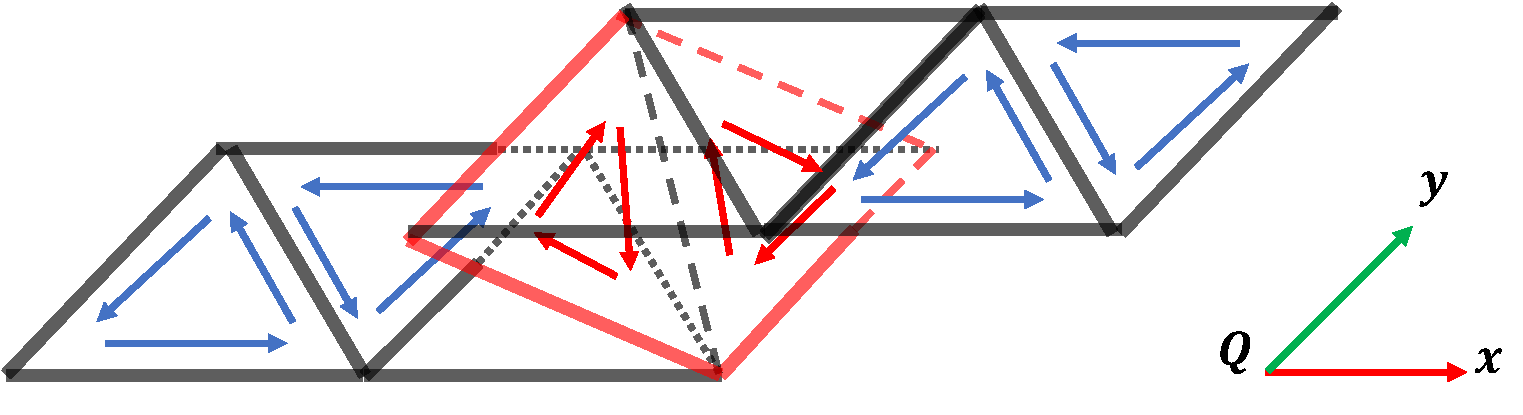
\includegraphics[width=\linewidth]{diagram/flip.pdf}
%\caption{The arrows show the orientation direction in the domain parametrized by $\mathbf{Q}$. Negative orientations are marked in red. It finally causes inverted faces in red in the quad mesh.}
%\label{fig:quadflip}
%\end{figure}
%Figure~\ref{fig:quadflip} shows that 
If the position field has triangles with negative orientation, they lead to inverted faces in the quad mesh. To ensure that there are no inverted faces in the output, each triangle should have nonnegative orientation, i.e.,
\begin{equation}
\text{det} \left[\mathcal{R}^u_{uv}\td_{uv},\;\mathcal{R}^u_{uw}\td_{uw}\right]\geq 0. \label{eq:quad-noflip}
\end{equation}
This constraint is similar to the consistent orientation constraint proposed by Bommes et al.~\cite{bommes2013integer}. Jakob et al.\ do not enforce this constraint, so their meshes can have inverted faces.

\paragraph*{Formulation.}
Combining Equations~\eqref{eq:quad-im2}, \eqref{eq:quad-consistent}, and~\eqref{eq:quad-noflip}, we formulate the position field problem as follows.
\begin{align*}
\minimize_{\p, \t} \quad & E_p(\p, \t)\\
\text{subject to} \quad & \mathcal{R}^u_{uv}\td_{uv} + \mathcal{R}^u_{vw}\td_{vw} + \mathcal{R}^u_{wu}\td_{wu} = 0 \quad \forall \Delta_{uvw} \in \mathcal{F},  \\
                   & \text{det} \left[\mathcal{R}^u_{uv}\td_{uv},\;\mathcal{R}^u_{uw}\td_{uw}\right]\geq 0 \quad \forall \Delta_{uvw} \in \mathcal{F}.
\end{align*}
This is a mixed-integer programming problem. Solving it directly is NP-hard and thus not generally scalable. Our method finds an approximate solution by first computing $\p^*$ and $\t^*$ without constraints, using Gauss--Seidel iterations \cite{jakob2015instant}, then computing $\d^*$ from $\t^*$ according to the definition, then adjusting $\d$ to enforce Equations~\eqref{eq:quad-consistent} and~\eqref{eq:quad-noflip}. To enforce Equation~\eqref{eq:quad-consistent}, we try to solve an integer programming problem, namely to
\begin{align}
\minimize_{\d} \quad & \lVert \d-\d^*\rVert_1 \label{eq:quad-formulation} \\
\text{subject to} \quad &
\mathcal{R}^u_{uv}\td_{uv} + \mathcal{R}^u_{vw}\td_{vw} + \mathcal{R}^u_{wu}\td_{wu} = 0 \quad \forall \Delta_{uvw} \in \mathcal{F}.\nonumber
\end{align}
We temporarily ignore the quadratic consistent orientation constraints~\eqref{eq:quad-noflip}. We describe an algorithm to solve this relaxed problem in Section~\ref{sec:quad-maxflow}.   In Section \ref{sec:quad-flip}, we describe heuristics to locally repair the inverted triangles and satisfy Equation~\eqref{eq:quad-noflip} without breaking the regularity constraints~\eqref{eq:quad-consistent}.  Finally, we re-optimize the position field in Section~\ref{sec:quad-postoptimize}.

\subsection{Removing Singularities from the Position Field}
\label{sec:quad-maxflow}

\begin{figure}

\begin{minipage}{0.6\linewidth}
\begin{align*}
\minimize_{\x} \quad & x_1 + 2x_2 + 3x_3 + x_4 +4x_5\\
\text{subject to} \quad & x_2-x_3=-5 \\
& x_5-x_2-x_1=-2 \\
& x_3+x_4-x_5=4 \\
& x_1-x_4=3 \\
& 0 \le x_1 \le 3 \\
& 0 \le x_2 \le 2 \\
& 0 \le x_3 \le 2 \\
& 0 \le x_4 \le 3 \\
& 0 \le x_5 \le 1 \\
& x_i \in \mathbb{Z} \quad \forall i
\end{align*}
\end{minipage}
\begin{minipage}{0.34\linewidth}
\centering
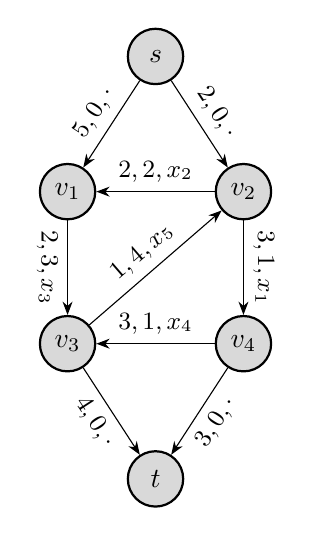
\begin{tikzpicture}[
mycircle/.style={
circle,
thick,
draw=black,
fill=gray,
fill opacity = 0.3,
text opacity=1,
inner sep=0pt,
minimum size=20pt},
myarrow/.style={-Stealth},
node distance=1.2cm and 0.6cm
]
\node[mycircle] (c1) {$s$};
      \node[mycircle,below left=of c1] (c4) {$v_1$};
      \node[mycircle,below right=of c1] (c2) {$v_2$};
      \node[mycircle,below=of c2] (c3) {$v_4$};
      \node[mycircle,below=of c4] (c5) {$v_3$};
      \node[mycircle,below right=of c5] (c6) {$t$};
      \foreach \i/\j/\txt/\p in {
      c1/c2/{$2,0,\cdot$}/above,
      c1/c4/{$5,0,\cdot$}/above,
      c2/c3/{$3,1,x_1$}/above,
      c3/c6/{$3,0,\cdot$}/below,
      c4/c5/{$2,3,x_3$}/below,
      c5/c6/{$4,0,\cdot$}/below,
      c5/c2/{$1,4,x_5$}/above,
      c3/c5/{$3,1,x_4$}/above,
      c2/c4/{$2,2,x_2$}/above}
       \draw [myarrow] (\i) -- node[sloped, \p, font=\small] {\txt} (\j);
\end{tikzpicture}
\end{minipage}

\caption{Left: an integer linear program in which all the variables are balanced.  Right: the corresponding minimum cost network flow problem.  The three symbols of the label on each edge represent the capacity, the cost, and the corresponding ILP variable, respectively. Under the full flow condition, these problems are equivalent.}
\label{fig:quad-maxflowexample}
\end{figure}

Equation~\eqref{eq:quad-formulation} is an integer programming problem (ILP), but we are able to approximate it as a \emph{minimum cost network flow} (MCF) problem, which is our key contribution. Efficient algorithms such as the network simplex method \cite{orlin1997polynomial} can be applied to find its optimal solution in polynomial time.

\paragraph*{Minimum Cost Flow.}
\label{sec:mincost}
% One zHowever, Instant Meshes solves the continuous relaxation without satisfying the integer constraints and already achieve promising results. Thus, it is promising to start from the continuous relaxation, and modify $\textbf{d}_p$ to satisfy all integer constraints.

%In minimum cost flow problem, let $G=\left<V, E\right>$ be the graph, $s, t \in V$ be the source and the sink respectively, $c: E \to \mathbb{N}$ be the capacity of the edge, and $\ell: E \to \mathbb{R}^+$ be the cost of the edge.  We want to find the best $f: E \to \mathbb{N}$ to maximize

We first show that we can reduce the following class of ILP problems to MCF problems. Given $\mathbf{A} \in \R^{n \times m}$, $\mathbf{b} \in \R^{n}$, $\varsigma_i \in \mathbb{Z}$, and $\mathbf{\omega} \in \R^{m}_+$, an ILP problem can be written as
\begin{equation}
\begin{split}
\minimize_{\mathbf{x} \in \mathbb{Z}^m} \quad & \mathbf{\omega}^\intercal \mathbf{x} \\
\text{subject to} \quad & \mathbf{Ax} = \mathbf{b} \\
& 0 \le x_i \le \varsigma_i \quad \forall i \in \{1, 2, \dots, m\}.
\end{split}
\label{eq:quad-ilp}
\end{equation}
Suppose that each column of the matrix $A$ contains one $+1$, one $-1$, and $n-2$ zeros. In other words, each variable $\mathrm{x}_i$ must appear exactly twice in the equality constraints, once with coefficient $+1$ and once with coefficient $-1$. For convenience, we say that a variable is \emph{balanced} if it satisfies this requirement. We claim that this ILP can be reduced to an MCF problem if all the variables are balanced.  

We begin by constructing a network graph $G = (V, E, c, w, s, t)$, in which $c: E \to \mathbb{R}$ is the capacity of each edge, $w: E \to \mathbb{R}$ is the cost of each edge, and $s$ and $t$ are the source and the sink nodes of the network, respectively.  For $i \in \{1, 2, \dots, n\}$, we add a node $v_i$ to $V$ corresponding to the $i$th equality constraint $\mathbf{A}_i \x = b_i$; we also add $s$ and $t$ to $V$. Then, for each variable $x_k$ and for $A_{ik}=-1$ and $A_{jk}=+1$, we create an edge $e_{ij}$ from node $v_i$ to $v_j$, which will carry a flow $f_{ij} = x_k$. The capacity of $e_{ij}$ is $c_{ij}=\varsigma_k$ and the cost of $e_{ij}$ is $w_{ij} = \omega_k$.  Finally, for each constraint $\mathbf{A}_i \x = b_i$, if $b_i>0$ we create a zero-cost edge from node $v_i$ to sink $t$ with capacity $c_{it}=b_i$, and if $b_i<0$ we create a zero-cost edge from source $s$ to node $v_i$ with capacity $c_{si}=-b_i$. Figure~\ref{fig:quad-maxflowexample} shows an example of an ILP and its equivalent MCF problem.

Solving the ILP in Equation \eqref{eq:quad-ilp} is equivalent to finding the minimum cost flow $f: E \to \mathbb{Z}$ of $G$ under the \emph{full flow condition}, in which flows of every outgoing edge from $s$ and every incoming edge to $t$ are required to reach their full capacity, i.e., $f_{si}=c_{si}$ and $f_{it}=c_{it}$ for every node $i$. After solving the MCF problem, we solve the ILP by setting each $x_k$ equal to the corresponding $f_{ij}$. These two problems are equivalent because of the \emph{flow conservation} condition: for each node, the sum of the flows entering the node is equal to the sum of the flows leaving it; that is, $\sum_{u} f_{uw}=\sum_v f_{wv}$ for all $w \in V$.  We have the following observations.
\begin{itemize}
\item The objective functions of the ILP and MCF are the same.
\item Each equality constraint with $b_i=0$ in the ILP is equivalent to the flow conservation condition at the corresponding node in the MCF network.
\item For each equality constraint with $b_i>0$ in the ILP, it is equivalent to the flow conservation condition at the corresponding node if the edge capacity from the node to $t$ is fully occupied, i.e., $f_{it}=c_{it}$. For $b_i<0$, the equivalence holds if the capacity of the edge from $s$ is fully occupied, i.e., $f_{si}=c_{si}$. 
\end{itemize}
Consider the example in Figure~\ref{fig:quad-maxflowexample}. The flow conservation condition at $v_1$ requires that $f_{s1} + f_{21} = f_{13}$. This is equivalent to the constraint $x_2 - x_3 = -5$ in the ILP when edge $(s, v_1)$ is at full capacity: $f_{s1} = c_{s1} = 5$. Therefore, a flow that satisfies the full flow condition corresponds to a feasible solution of Equation~\eqref{eq:quad-ilp}, while the identical objective functions imply that a solution optimal for one is optimal for the other.

Let ${\textbf{t}}^*$ be a solution obtained from the algorithm of Jakob et al.\ that does not respect all the constraints from Section~\ref{sec:quad-constraints}. We compute ${\d}^*$ from ${\textbf{t}}^*$. Our first goal is to satisfy the regularity constraints~\eqref{eq:quad-consistent} with a minimum change to ${\textbf{d}}^*$ per objective~\eqref{eq:quad-formulation}. When we enforce the constraints, it will cause a change $\delta \d={\textbf{d}}-{\textbf{d}}^*$ to the integer offsets. To satisfy the requirement~\eqref{eq:quad-ilp} that the variables are constrained to be nonnegative, we split $\delta \d_e$ into two nonnegative variables $\delta \d_e = \delta \d^+_e - \delta \d^-_e$.  Our aim is to choose $\delta \d^+_e$ and $\delta \d^-_e$ for all $e \in \mathfrak{E}$ to
\begin{align}
\minimize \quad & \sum_{e \in \mathfrak{E}} \delta\d^+_e+\delta\d^-_e\label{eq:quad-mincost}\\
\text{subject to} \quad & \mathcal{R}^u_{uv}{\textbf{d}}_{uv}+\mathcal{R}^u_{vw}{\textbf{d}}_{vw}+\mathcal{R}^u_{uw}{\textbf{d}}_{wu}=\textbf{0} \;\;\;\forall \Delta_{uvw} \in \mathcal{F}, \label{eq:quad-mincost-cons} \\
& {\d}_e = {\textbf{d}}^*_e +\delta \d^+_e - \delta \d^-_e \quad\forall e \in \mathfrak{E}, \notag \\
& \mathbf{0} \le \delta \d^+_{e} \le \HH_{e}^+  \quad \forall e \in \mathfrak{E}, \notag \\
& \mathbf{0} \le \delta \d^-_{e} \le \HH_{e}^-  \quad \forall e \in \mathfrak{E}, \notag \\
&       \delta \d^+_e, \, \delta \d^-_e \in \mathbb{Z}^2 \quad \forall e \in \mathfrak{E}, \notag
\end{align}
where $\HH_{uv}^+$ and $\HH_{uv}^-$ are the maximum allowed modification for ${\d}$ in the positive direction and the negative direction, respectively.  Initially, we set $H^+_{uv}$ and $H^-_{uv}$ so that the $\d_{uv} \in [-2,2]^2$. Then we repeatedly increase this limit until the corresponding MCF problem is feasible. The reason we want to keep $|\d_{uv}|_\infty$ as small as possible is that if there exists a long edge in the integer offsets, we need to subdivide it (later on in this section), which creates more vertices.  This ILP has the form of Equation~\eqref{eq:quad-ilp} and satisfies most of the prerequisites to be cast as an MCF problem, but it does not satisfy the balance condition.

\paragraph*{Balancing Variables.}
To use the MCF formulation to solve Equation \eqref{eq:quad-mincost}, we need to balance the variables in Equation \eqref{eq:quad-mincost-cons},  making each variable appear twice with opposite signs.  For a manifold triangle mesh, each edge adjoins exactly two triangles except for the edge at the boundary. To make each variable appear exactly twice in Equation \eqref{eq:quad-mincost-cons}, we simply fix $\delta{\textbf{d}}_{e}$ to be a constant for each $e \in \mathcal{E}$ at the boundary.

\begin{figure}
\centering
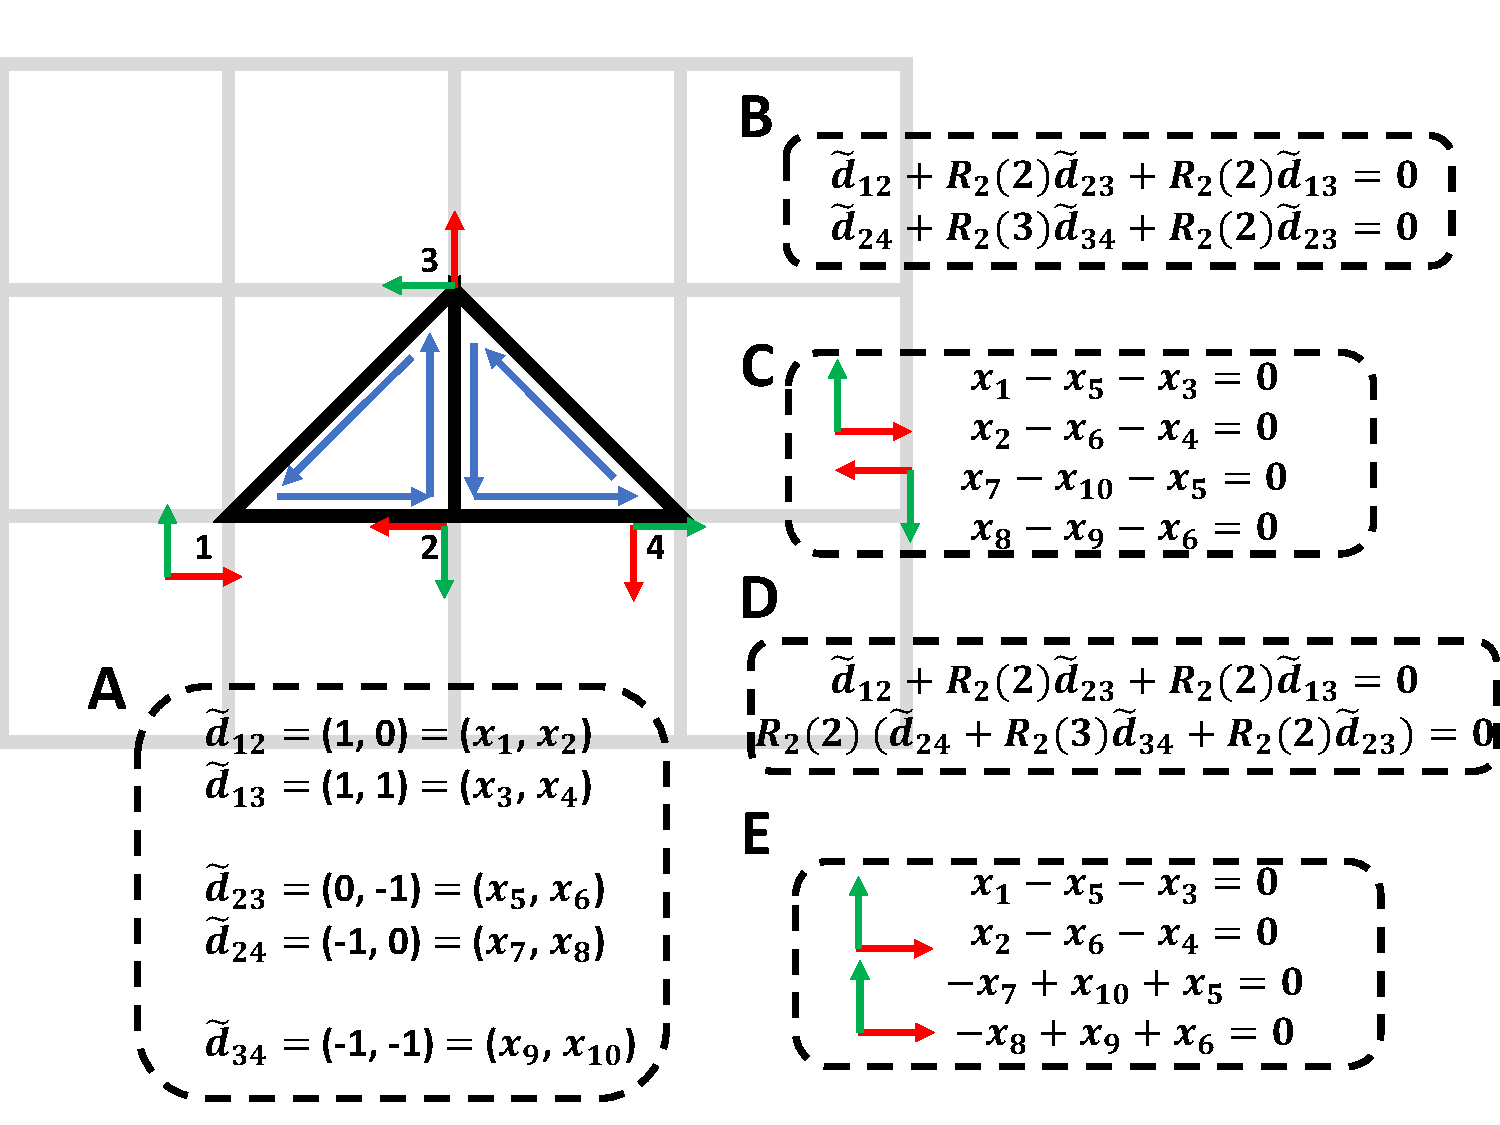
\includegraphics[width=0.6\linewidth]{quadriflow/diagram/balance.pdf}
\caption{This example shows why variables may not be balanced. Panel A shows the ten integer variables corresponding to the five edges of two adjacent triangle elements. Their regularity constraints are shown on Panel B in the vector form and Panel C in the scalar form, in which variables $x_5$ and $x_6$ are not balanced.  By rotating the second equation of the right triangle through $180^\circ$ in Panel D, $x_5$ and $x_6$ become balanced as shown in Panel E.}
\label{fig:quad-balance}
\end{figure}

Some variables may not be balanced initially, but we can balance them by a simple 2D rotation. Suppose $\td_e$ appears in two regularity constraints in Equation~\eqref{eq:quad-mincost-cons} with coefficients $\mathbf{R}_2(k_1)$ and $\mathbf{R}_2(k_2)$. We can rotate the second equation by multiplying it by $\mathbf{R}_2(k_1-k_2+2)$ so that the second coefficient becomes $-\mathbf{R}_2(k_1)$ and balances the two signs of $\td_e$. Figure~\ref{fig:quad-balance} shows an example containing two triangles, in which the frame of each vertex is marked. Panel A shows the variables as ${\td}$. We show the regularity constraints, i.e., Equation~\eqref{eq:quad-mincost-cons}, in Panel B as the vector form and in Panel C as the scalar form. The variable ${\textbf{d}}_{23}$ (or variables $x_5$ and $x_6$) has two negative signs and thus is not balanced. By rotating the second equation $180^\circ$ as Panel D illustrates, we are able to balance ${\textbf{d}}_{23}$.

%\begin{figure}
%\centering
%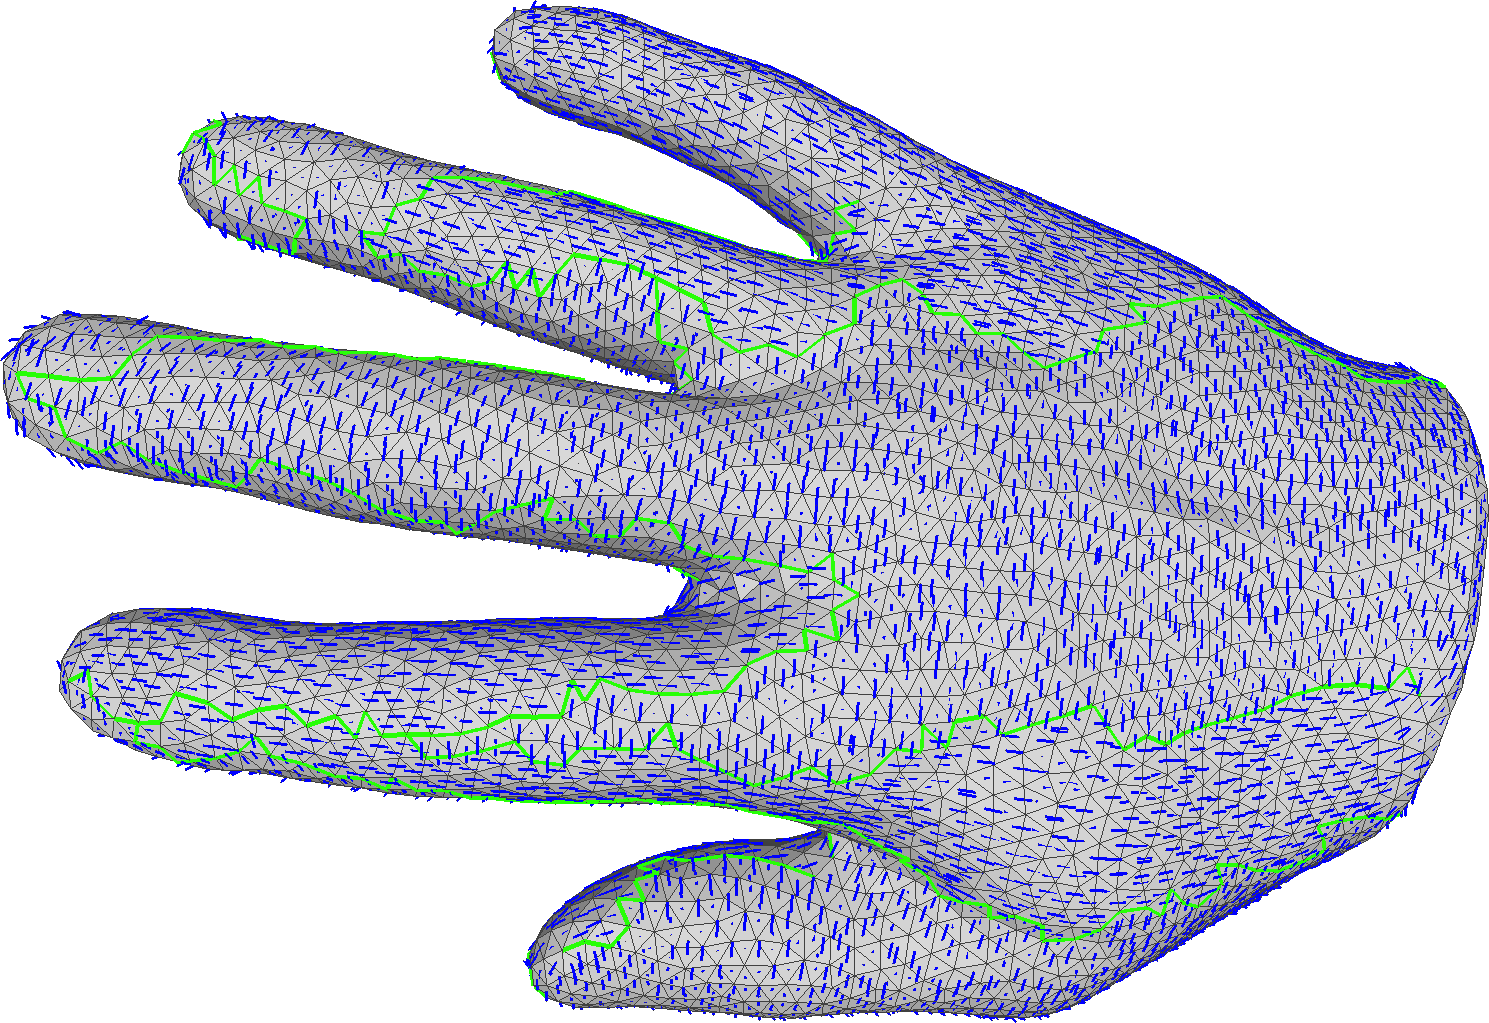
\includegraphics[width=0.99\linewidth]{diagram/boundary.png}
%\caption{The hand model is visualized with unbalanced edges marked with green line, and the x-axes with blue lines of frames where equality constraints are measured for each triangle.}
%\label{fig:vis-boundary}
%\end{figure}

To balance as many variables as possible, we arbitrarily pick a triangle as the reference (the root of the search tree) and do a breadth-first search (BFS) to visit other triangles. For each pair of equations corresponding to the two adjacent triangles along the search tree, we rotate the second equation to balance their shared variables. For the edges that are not on the BFS search tree, the balanced condition is not guaranteed.  We fix those unbalanced variables as constants so that all mutable variables are balanced.

%We observe that these rotations to balance variables are also geometrically meaningful. Recall that we rotate equations to balance variables. The rotation through a specific angle to an equation can also be viewed as changing the frame of measurement for integer offsets for its corresponding triangle, where the changed frame can be derived by rotating the original frame through the same angle around the normal axis\jw{Is it not clear?}. To illustrate this implicit meaning, we visualize the boundary edges in green, and the frame of measurement for each triangle $\Delta_{uvw}$ in blue by applying the corresponding rotation to $\mathbf{q}_u$ in Figure~\ref{fig:vis-boundary}. We notice that the frame of measurement is consistent between faces with balanced variables, which is reasonable because the directions of the integer offsets are opposite for the shared edge in adjacent triangles. This also implies the insight for our rotation operation: We balance ${\d}_e$ by measuring the integer offset of edge $e$ in two adjacent faces with a locally consistent frame. \jw{add this paragraph!}

\paragraph*{Feasibility Condition.} Fixing unbalanced variables to $\td^*$ as constants may lead to an infeasible ILP problem. One necessary condition for feasibility is $\sum_{i=1}^n b_i=0$ for $\mathbf{b}$ in Equation \eqref{eq:quad-ilp}.  To prove this, we add all the equality constraints together $\sum_{i=1}^n \mathbf{A}_i \x = \sum_{i=1}^n b_i$, and because each column of $\mathbf{A}$ contains one $+1$, one $-1$ and $n-2$ zeros, the left hand side is equal to zero, so is $\sum_{i=1}^n b_i$.  From the view of MCF, this requires the outbound capacity of the source $s$ equal to the inbound capacity of the sink $t$.

To guarantee $B:=\sum_{i=1}^n b_i=0$, we apply the following greedy strategy to determine $\delta \d_{uv}$ for unbalanced edges and boundary edges.  Initially, we set $\delta \d_{uv}=0$ for all unbalanced and boundary edges.  Next, we randomly select one of these edges and change it in the direction to decrease the magnitude of $B$. This process is repeated until $B=0$. This strategy is based on the fact that incrementing/decrementing a variable for a boundary edge changes $B$ by one, whereas incrementing/decrementing a variable for an unbalanced edge changes $B$ by two. Note that $B=0$ can always be achieved because we can at least let $\td_{uv}=0$ for all unbalanced edges and boundary edges $(u,v)$ to satisfy it, i.e., setting $\delta \d_{uv} = -\td^*_{uv}$.

Now, we show the sufficient condition for the feasibility of the ILP considering its equivalent MCF problem. Let $C^-:=\sum_u c_{su}$ be the outbound capacity of the source and $C^+:=\sum_v c_{vt}$ be the inbound capacity of the sink.  The following theorem states that with proper assumption, the full flow condition in the MCF formulation is always achievable.
\begin{theorem}
Given a network $G=(V, E, c, w, s, t)$, if $C^+=C^-$, all the internal vertices $V \backslash \{s,t\}$ are strongly connected (a vertex $v_a$ is strongly connected to $v_b$ if there exist two paths, one from $v_a$ to $v_b$ and another from $v_b$ to $v_a$), and $c_{uv} \ge C^+$ for all $(u,v) \in E$ in which $u,v \notin  \{s,t\}$, then the maximum flow $f$ satisfies the full flow condition.
\label{th:connect}
\end{theorem}

\begin{proof}
We prove it by contradiction. Given a network $G=(V, E, c, w, s, t)$ where $V \backslash \{s,t\}$ are strongly connected, we assume $f$ does not satisfy the full flow condition.  Because the edge capacity is larger than $C^+$, the flow on any internal edge $(u,v)$ is smaller than the capacity.  This means that the connectivity of the residual network of $f$ remains unchanged.  Therefore, $V \backslash \{s,t\}$ is still strongly connected in the residual network. Also because $C^+=C^-$ and the full flow condition is not satisfied, $s$ and $t$ must be connected to $V \backslash \{s,t\}$ in the residual network.  So there exists an augmenting path from $s$ to $t$, which contradicts the assumption.
\end{proof}

Fortunately, we guarantee the strong connectivity in the MCF network: Because we use BFS to balance variables, any adjacent triangles on the search tree share an edge $e$ with balanced ${\d}_e$. Therefore as long as the triangle mesh $\mathcal{M}$ is connected, the corresponding nodes of the adjacent triangles in the flow networks are connected. Because BFS reaches all triangles in the mesh, the corresponding nodes in the flow networks are strongly connected.  In addition, according to the way we construct the network, we have $C^+ = \sum_{b_i > 0}b_i$ and $C^- = -\sum_{b_i < 0} b_i$.  Thus, $B=0$ implies $C^+ = C^-$. By using the above theorem, we can guarantee the achievement of a full flow by computing the maximum flow once we have $c_{uv} \geq C^+$ for all edges $(u,v) \in E$, or large enough $\HH_{uv}$ in the ILP (Equation~\ref{eq:quad-mincost-cons}).

\begin{figure}
\centering
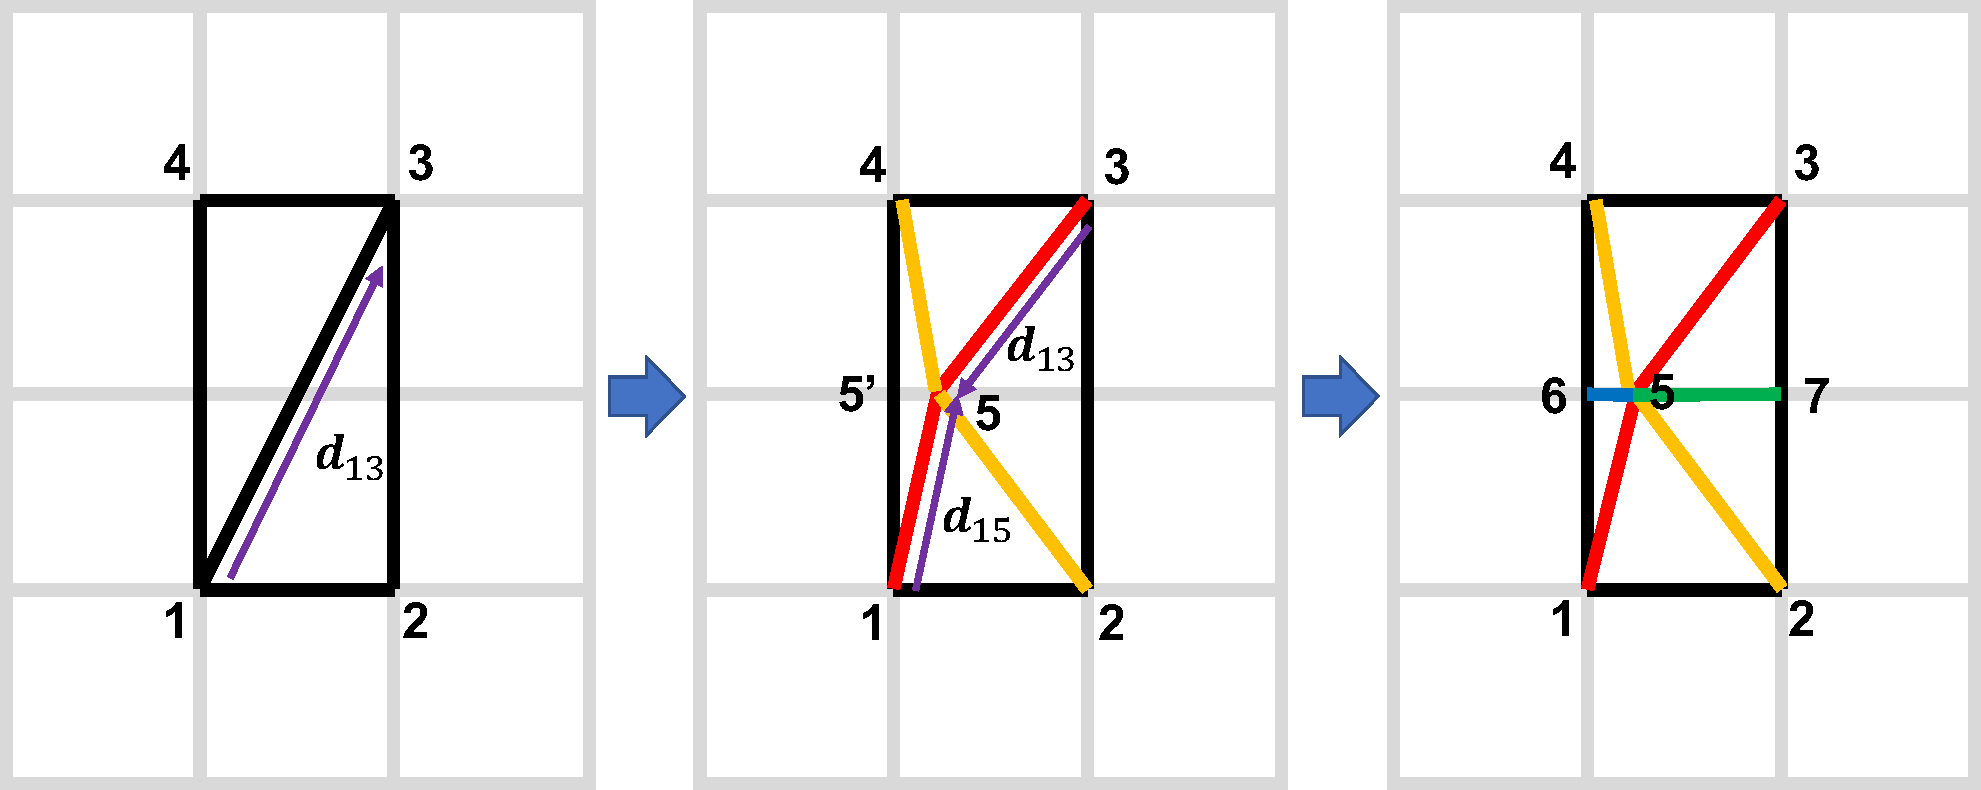
\includegraphics[width=0.6\linewidth]{quadriflow/diagram/subdivide.pdf}
\caption{Subdivision example. At the left, there are initially three long edges ${\textbf{d}}_{13}=(1,2)$, ${\textbf{d}}_{14}=(0,2)$ and ${\textbf{d}}_{23}=(0,2)$. We first subdivide ${\textbf{d}}_{13}$ as ${\textbf{d}}_{15}=(0,1)$ and ${\textbf{d}}_{35}=(-1,-1)$, as shown in the middle. Note that the actual location of $v_5$ is at $v_{5'}$, but we draw it at $v_5$ for clarity. Finally, we subdivide ${\textbf{d}}_{14}$ and then ${\textbf{d}}_{23}$. As a result, all edges have $\|{\textbf{d}}\|_{\infty}\leq 1$.}
\label{fig:quad-subdivide}
\end{figure}

\paragraph*{Summary.}
To remove position singularities, we first BFS triangles on the mesh to rotate the corresponding equations to balance variables. We fix boundary and unbalanced variables, and randomly modify them to achieve $\sum_{i=1}^n b_i=0$. Then, we build an equivalent MCF network. We set all edge capacities $c_{uv}$ (or $H^-_{uv}=H^+_{uv}$ in the ILP) so that $\d_{uv} \in [-2,2]^2$ and run an MCF solver. If it returns infeasible, we retain the flow value $f$ for each edge and repeatedly increase the capacity until the problem is feasible.

%\begin{algorithm}
%    \SetKwInOut{Input}{input}
%    \SetKwInOut{Output}{output}
%
%    \Input{Mesh $\mathcal{G}=(\mathcal{V},\mathcal{E})$, normal vectors $\n$, orientation field $\q^*$, and Position Field $\p$}
%    \Output{${\textbf{d}}$  that satisfies the no-position singularity constraints}
    %\ForEach{$\mathcal{G}' \in$ connected components of $\mathcal{M}$}{
%        \ForEach{$(u,v)\in\mathcal{E}$} {
%            Compute ${\textbf{d}}_{uv}$ based on $\q_u,q_v,\p_u,\p_v$
%        }
%        Balance ${\textbf{d}}$ with disjoint-set forests\\
%        Randomly modify unbalanced variables until $C^+=C^-$\\
%        Build $G=\left<V,E,s,t\right>$\\
%        \For {$w\leftarrow 2$ to $C^+$} {
%            Set all edges' capacity as $w$ except $\left<s,*\right>$ and $\left<*,t\right>$\\
%            $f\leftarrow flow(G)$\\
%            \If {$f=C^+$} {
%                \textbf{Break}
%            }
%        }
%        Update variables according to the flow
    %}
%    \caption{Remove Position Singularity}
%    \label{alg:flow}
%\end{algorithm}

%\begin{figure}
%\centering
%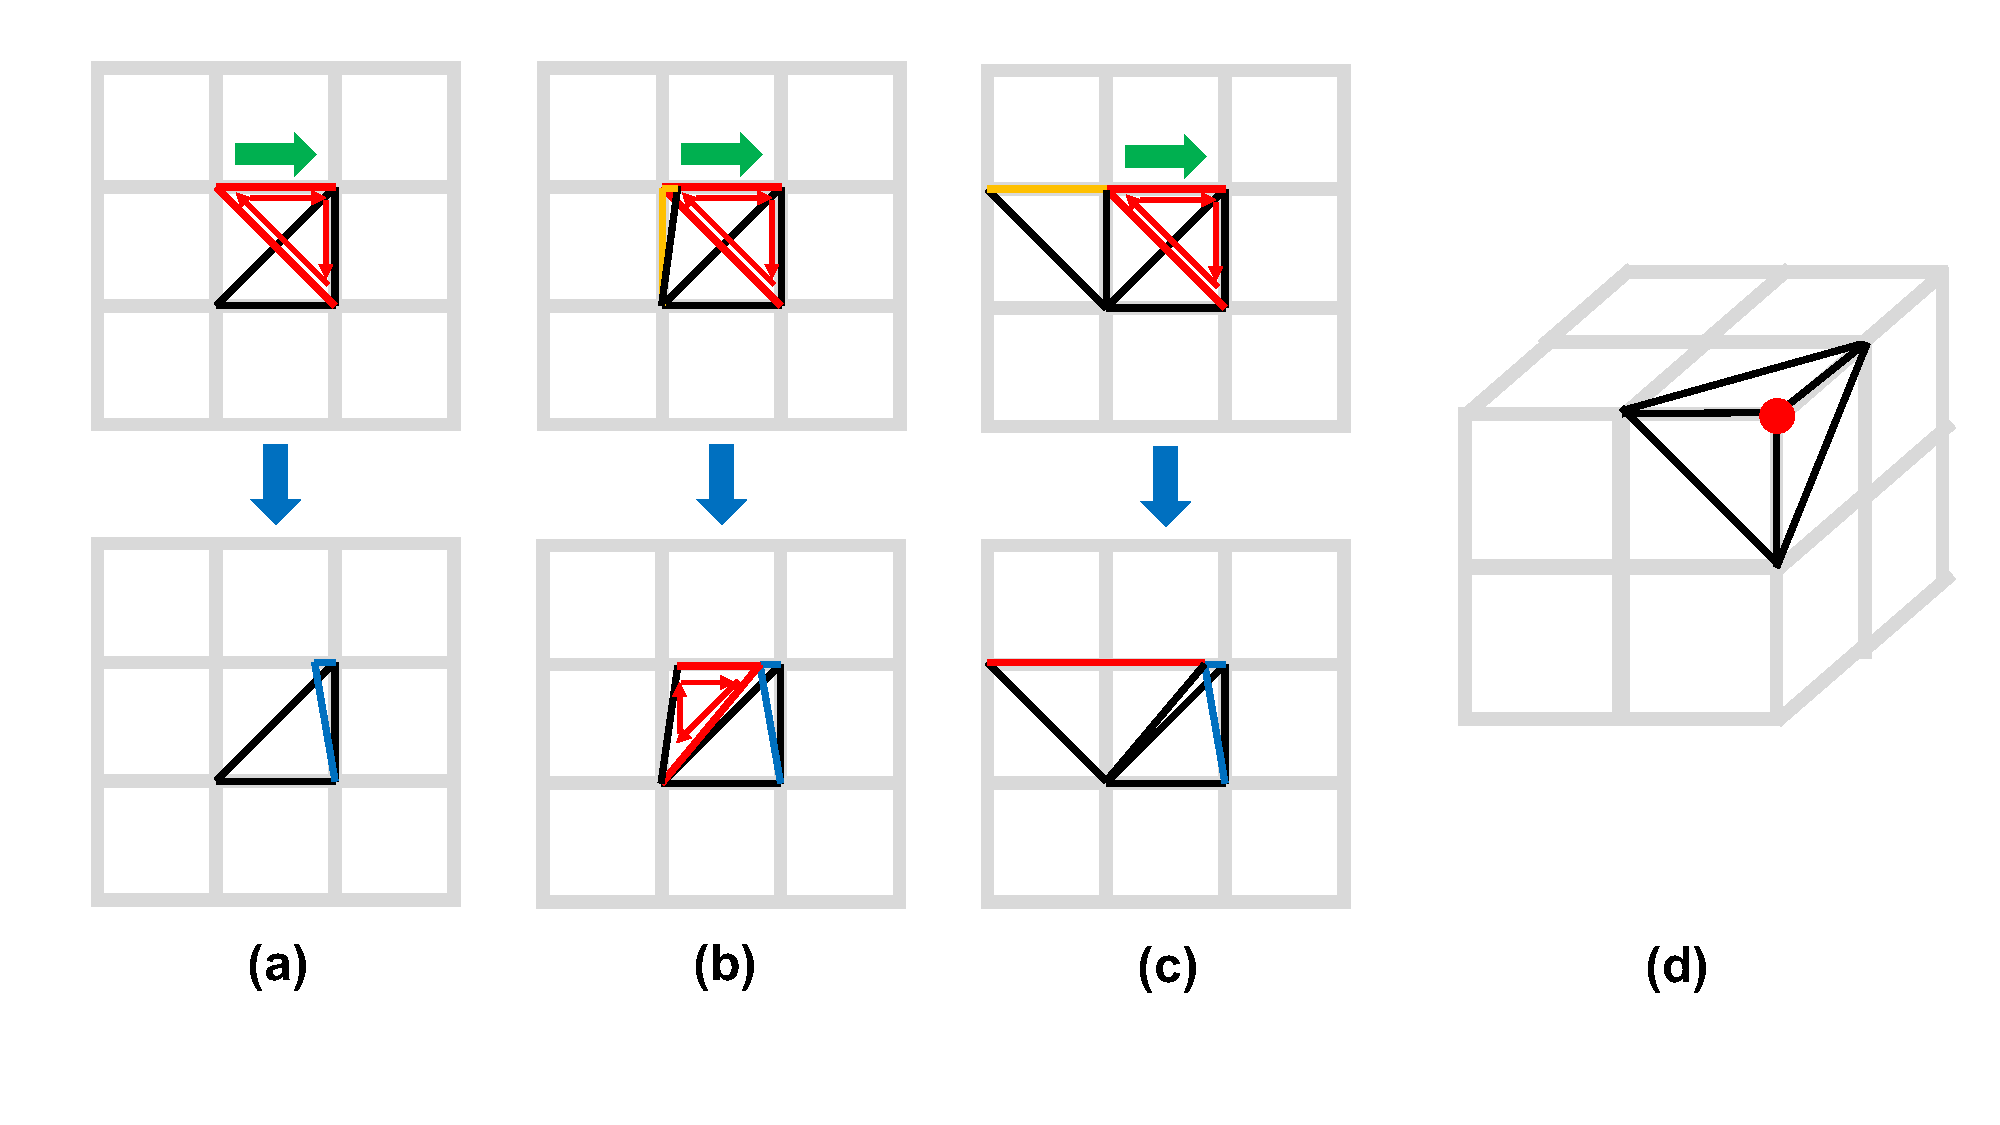
\includegraphics[width=\linewidth]{diagram/flipexample.pdf}
%\caption{Move vertex to reduce triangle inversion. (a) shows how vertex can be moved to shrink the inverted triangle. (b) Vertex movement can cause a new inversion in neighboring triangles, marked as orange in the first row and red in the second row. (c) Vertex movement can produce long edges, marked as orange in the first row and red in the second row. (d) Any movement of the vertex at an orientation singularity will violate equality constraints (equation~\eqref{eq:quad-consistent}).}
%\label{fig:flipexample}
%\end{figure}

\paragraph*{Multi-Resolution MCF.}
Under many scenarios, the required density of the quad mesh is significantly lower than the density of the input triangle mesh. This means that most of ${\textbf{d}}$ will finally be zero. Therefore, we are able to accelerate the MCF algorithm with a multi-resolution structure.

For each resolution, we build a coarser network by removing approximately half of zero edges ($\td^*_e=\textbf{0}$) to reduce the number of variables.  Consider a general case where the regularity constraints are satisfied for two equations corresponding to $\Delta_{abc}$ and $\Delta_{aef}$ sharing the edge $a$. The equation for $\Delta_{abc}$ can be written
\begin{equation*}
R_a {\textbf{d}}_a + R_b {\textbf{d}}_b + R_c {\textbf{d}}_c = 0.
\end{equation*}
When ${\textbf{d}}_a=\textbf{0}$, we can replace ${\textbf{d}}_b$ by ${\textbf{d}}_b=-R_b^{-1}R_c{\textbf{d}}_c$. Therefore, we can simplify the set of regularity constraints by a collapse operation: Remove the variable $\td_a$ and the two constraints for $\Delta_{abc}$ and $\Delta_{aef}$, and replace ${\textbf{d}}_b$ and ${\textbf{d}}_e$ with $-R_b^{-1}R_c{\textbf{d}}_c$ and $-R_e^{-1}R_f{\textbf{d}}_f$.

%This collapse operation is safe for the MCF requirement, that is, this operation maintains that all variables appear twice and are balanced. It also won't violate the full flow condition.
\begin{figure}
\centering
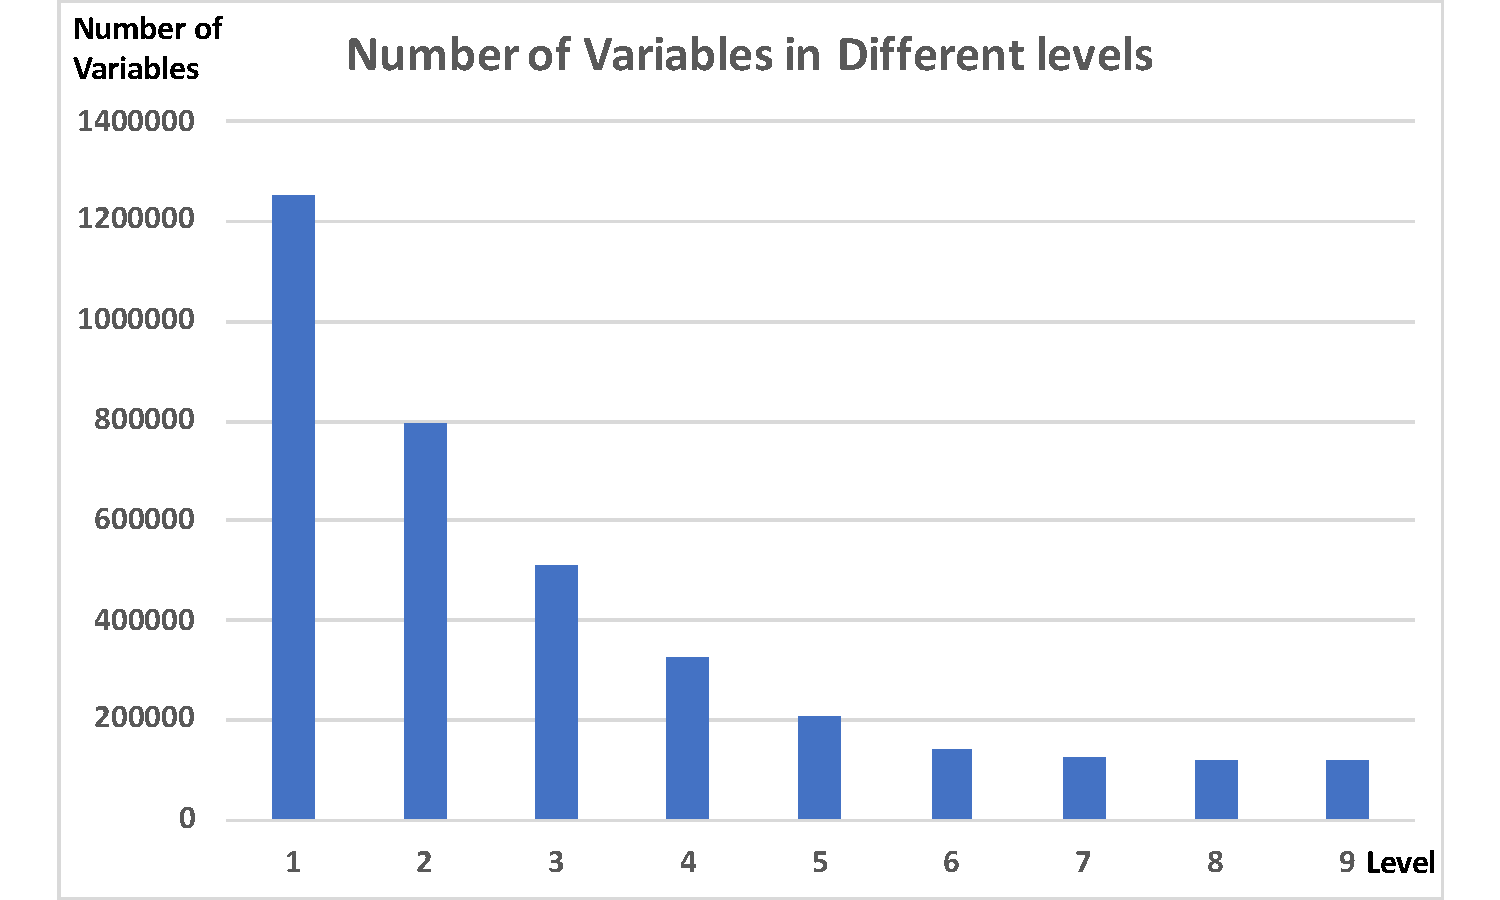
\includegraphics[width=0.6\linewidth]{quadriflow/diagram/hierarchy.pdf}
\caption{Number of variables at each level of our multi-resolution structure.}
\label{fig:quad-hierarchy}
\end{figure}

To build a hierarchy structure, we loop over all the edges with $\td_e=\textbf{0}$ at each resolution and collapse them if two corresponding equality constraints of the zero-edge are already satisfied. Once we remove the variable for one edge, we do not allow the collapse operation on adjacent edges at the same level. Figure~\ref{fig:quad-hierarchy} shows the number of variables for each level with our collapse operation. We first compute the flow at the lowest resolution and then propagate the change of variables to the higher resolution until the full flow condition is satisfied.  We keep the edge capacity to be two in the multi-resolution solver and only increase it if the full flow condition cannot be satisfied in the highest resolution. In practice, we usually can solve most singularities at the lowest resolution, where the number of variables is less than one-tenth of the number of variables in the original (highest) resolution.  

In the beginning, we use the network simplex implementation from the LEMON library \cite{dezsHo2011lemon} to solve the MCF at the lowest resolution.  This resolves most of the singularities with minimum change of $\td$.  For further trials with large networks, we approximate the MCF problem as a maximum flow problem for efficiency.  We use the Boykov--Kolmogorov algorithm~\cite{boykov2004experimental} if the number of remaining unsatisfied regularity constraints is greater than 10, and use the Edmonds--Karp algorithm~\cite{edmonds1972theoretical} otherwise.  The maximum flow approximation sacrifices some optimality of Equation \eqref{eq:quad-mincost}, but it greatly improves the efficiency and works well in practice, as Section~\ref{sec:quad-methodology} will demonstrate.

\paragraph*{Subdivision on Integer Offsets.}
After the Multi-Resolution MCF, $\|{\textbf{d}}_{uv}\|_{\infty}$ might be greater than $1$ in order to satisfy the full flow condition.  This will complicate the mesh extraction stage later. Therefore, we subdivide the integer offsets of those long edges by adding a midpoint and two new edges. Because we require the lengths of the edges to be integers, the two subdivided edges of ${\textbf{d}}_{uv}$ are computed as ${\textbf{d}}_{uv}\;\text{div}\;2$ and $(-{\textbf{d}}_{uv}+{\textbf{d}}_{uv})\;\text{div}\;2$. Figure~\ref{fig:quad-subdivide} shows an example: the long edge ${\textbf{d}}_{13}=(1,2)$ is divided into ${\textbf{d}}_{15}=(0,1)$ and ${\textbf{d}}_{35}=(-1,-1)$, then $\td_{14}$ and $\td_{23}$ are subdivided.

\subsection{Eliminating Inverted Normals}
\label{sec:quad-flip}
To enforce the consistent orientation constraint in Equation~\eqref{eq:quad-noflip}, we employ a two-stage method.  First, a greedy algorithm scans the triangle elements in the mesh and iteratively shrinks the inverted triangles. After that, we locally model Equations~\eqref{eq:quad-consistent} and~\eqref{eq:quad-noflip} as a Boolean satisfiability problem and try to resolve the remaining inversions with an SAT solver.  Using this strategy, we are able to generate an inversion-free quad mesh for many testing data, but this is not always guaranteed due to the NP-completeness of the Boolean satisfiability problem.

\paragraph*{Greedy Method.}
One way to shrink an inverted triangle is to move one of its vertices to another. To move a vertex from $u$ to $v$, we set ${\d}_{uv}=0$ and modify $u$'s adjacent edges ${\d}_{uw}$ for all $(u,w)\in\mathfrak{E}$ accordingly to maintain the regularity constraints in Equation~\eqref{eq:quad-consistent}.  This operation locally changes the adjacent edges, and thus the area of the adjacent triangles. We scan all the edges of inverted triangles and shrink an edge only if it does not produce long edges ($\|d^*\|>1$) and reduces the total inverted area.  Our algorithm terminates until no further movement is feasible. This greedy algorithm can efficiently remove most of the inverted triangles. We observe that the remaining inversions are normally located near the orientation singularities.

\paragraph*{Reduction to SAT.}
To solve the remaining tough inversions,  we model it as a Boolean satisfiability (SAT) problem.  An SAT problem aims at finding an assignment to satisfy a given Boolean equation.  Although the SAT problem has been proven to be NP-complete, researchers have built efficient SAT solvers based on sophisticated heuristics that are able to solve practical problems with tens of thousands of variables.  To turn the constraints in Equations~\eqref{eq:quad-consistent} and~\eqref{eq:quad-noflip} to a Boolean equation, we represent each integer vector variable $\td_{uv}$ with nine Boolean variables $D^{\x}_{uv}$, where $\x \in \mathbf{S} := \{-1, 0, +1\}^2$ represents the nine possible values of the integer vector as these values are guaranteed to be in $\{-1, 0, +1\}$ after the subdivision stage.  The relationship between the integer variable and Boolean variable is
\[
\td_{uv}=\x \Longleftrightarrow D^{\x}_{uv}= \mathbf{true}
\]
for all $(u,v)\in\mathfrak{E}$ and $\x \in \mathbf{S}$.  Then we turn the constraints in Equations \eqref{eq:quad-consistent} and \eqref{eq:quad-noflip} into Boolean expressions in conjunctive normal form (CNF). CNF is a list of \emph{clauses} that need to be satisfied simultaneously, and each clause contains a list of variables connected by OR operators.  For each $\Delta_{uvw} \in \mathcal{F}$, we add the following clauses to our SAT solver: 
\begin{align*}
\lnot D^{\x}_{uv} \lor \lnot D^{\y}_{vw} \lor \lnot D^{\z}_{wu} \quad &\forall \x,\y,\z\in \S:\x+\y+\z\ne \mathbf{0}, \\
\lnot D^{\x}_{uv} \lor \lnot D^{\y}_{uw} \quad &\forall \x,\y\in \S: \mathrm{det} \left[ \x,\, \y \right] \le 0.
\end{align*}
The first Boolean equation enforces the regularity constraint and the second Boolean equation enforces the consistent orientation constraint.  The above representation is more for notation It is a little bit redundant because it needs 9 Boolean variable per integer offset.  We can reduce that to 6 Boolean variables by splitting the dimension of $\x$ for $D^{\x}_{uv}$ so that $D^{\x}_{uv}=:D^{x_1}_{uv}\land D^{x_2}_{uv}$, where $\x=(x_1, x_2)$.

In practice, we find that most triangle inversion problems can be solved locally. That is, it is sufficient to only change the geometry of the nearby regions of the inverted triangles.  So we iteratively increase the diameter of the mutable $\td$ until the resulting SAT problem is feasible or the SAT solver times out.  In our implementation, we use the open-source SAT solver \cite{liang2016learning}.  % After enforcing the consistent orientation constraints, we obtain a regular and inversion-free integer offset ${\textbf{d}}^{\star}$.

\subsection{Updating the Continuous Positions}
\label{sec:quad-postoptimize}

To make the real-valued variables of the position field consistent with our regularized, inversion-free integer offsets ${\textbf{d}}^{\star}$, we re-optimize $\p$ by minimizing the sum of squared differences between the actual and the desired distances,
\begin{equation}
E_{p}(\textbf{p}) = \sum_{(u, v) \in \mathcal{E}} ||\textbf{p}_v-\textbf{p}_u-\rho(\mathbf{O}_u\td_{uv}^{\star})||_2^2,
\label{eq:quad-post}
\end{equation}
where $\rho(\mathbf{O}_u\td_{uv}^{\star})$ is the desired 3D translation from vertex $u$ to $v$.
As with the method in Section~\ref{sec:quad-instantmesh}, for each vertex $u \in \mathcal{V}$, we restrict $\mathbf{p}_u$ to lie on $u$'s tangent plane.  This is a linear least-squares problem, easily and efficiently solvable.

Our re-optimization can be made to preserve sharp edges in the triangle mesh. We call an edge in $\mathcal{E}$ ``sharp'' if the angle between the two adjoining triangles' normals exceeds a user-specified threshold. If vertices on sharp edges are permitted to move in the tangent plane, sharp features may be lost, as Figure~\ref{fig:quad-fandisk}(a) shows. Thus, for a vertex $v\in\mathcal{V}$ on a sharp edge, we further constrain $\mathbf{p}_v$ to move only along the edge's affine hull. This constraint is easily incorporated into the linear least-squares problem. Figure~\ref{fig:quad-fandisk}(b) shows that this constraint yields better results.

\begin{figure}
\centering
\begin{minipage}{0.45\linewidth}
\centering
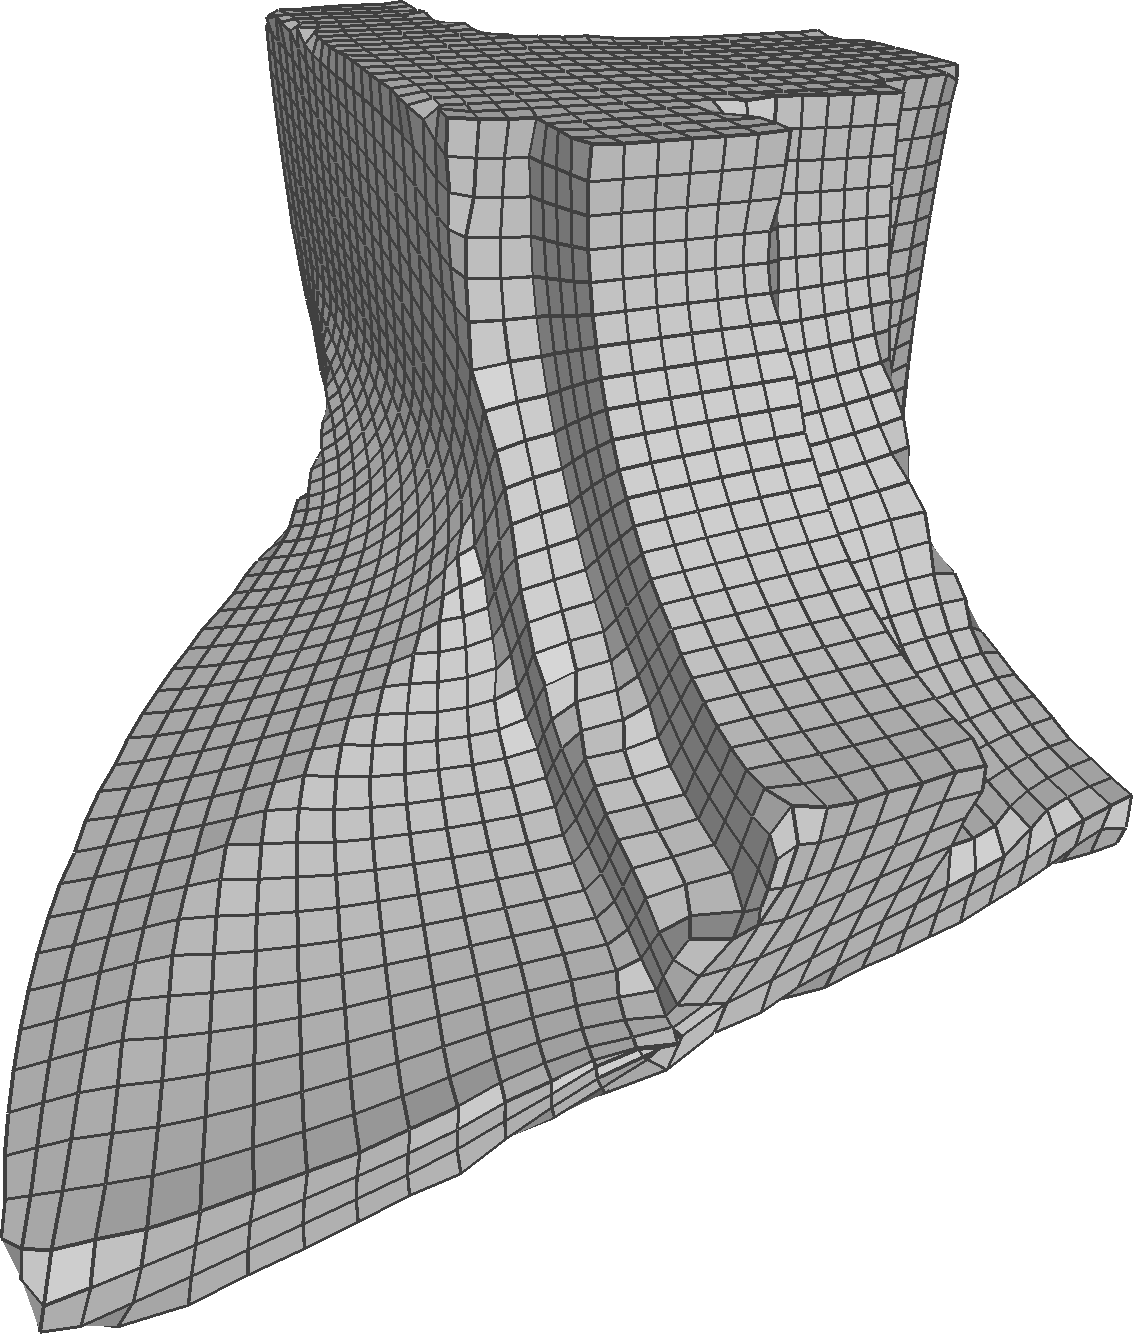
\includegraphics[height=0.6\linewidth]{quadriflow/result/fandisk00.png}\\
(a) Only tangential constraints
\end{minipage}
\begin{minipage}{0.45\linewidth}
\centering
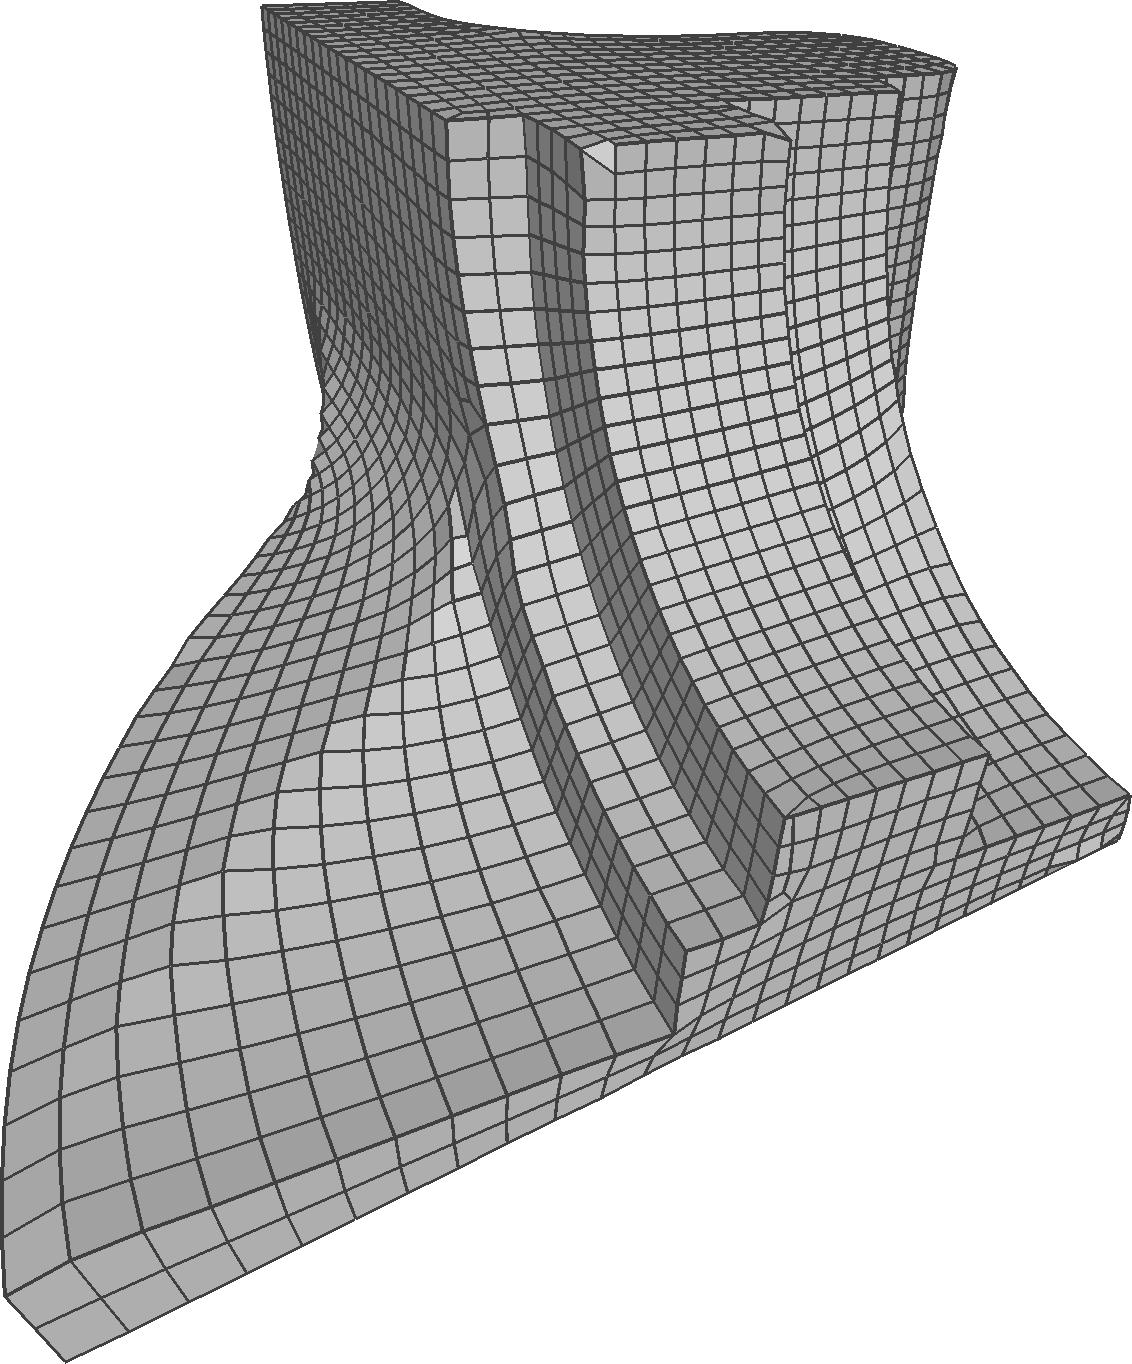
\includegraphics[height=0.6\linewidth]{quadriflow/result/fandisk01.png}\\
(b) With sharp edge constraints
\end{minipage}

\caption{(a) The tangent plane restriction does not suffice to preserve sharp edges. (b) Line constraints preserve sharp features better.}
\label{fig:quad-fandisk}
\end{figure}

\subsection{Quad Mesh Extraction}
\label{sec:quad-quadextraction}

Our quad mesh extraction algorithm is simpler than that of Jakob et al.~\cite{jakob2015instant}. Because of the subdivision routine described in Section~\ref{sec:quad-maxflow}, our position field (specified by $\p^{\star}$ and ${\textbf{d}}^{\star}$) does not have large integer translations (long edges); specifically, $|{\textbf{d}}^{\star}|_{\infty} \leq 1$. Moreover, as our position field has no singularities, each non-degenerate face is a right-angled isosceles triangle with one hypotenuse and two legs, and two triangles sharing the hypotenuse form a quad.  Hence our mesh extraction algorithm is straightforward: first, collapse all zero-length edges ($e$ for which ${\textbf{d}}_e^{\star} = \textbf{0}$). Then for each hypotenuse edge ($|{\textbf{d}}_e^{\star}|_1 = 2$), extract the quad for its two neighboring triangles. Because we enforce consistent orientation constraints, the quad mesh thus extracted is nearly always manifold. %If the non-manifold edge does exist, we duplicate edge to avoid it.

By comparison, the mesh extraction method for Instant Meshes~\cite{jakob2015instant} must cope with corner cases such as long edges, inverted triangles, and position field singularities. Figure~\ref{fig:quad-fail-face} gives an example for which their implementation has difficulty with complex geometry, whereas ours produces the correct topology.

\begin{figure}
\centering
\begin{minipage}{0.49\linewidth}
\centering
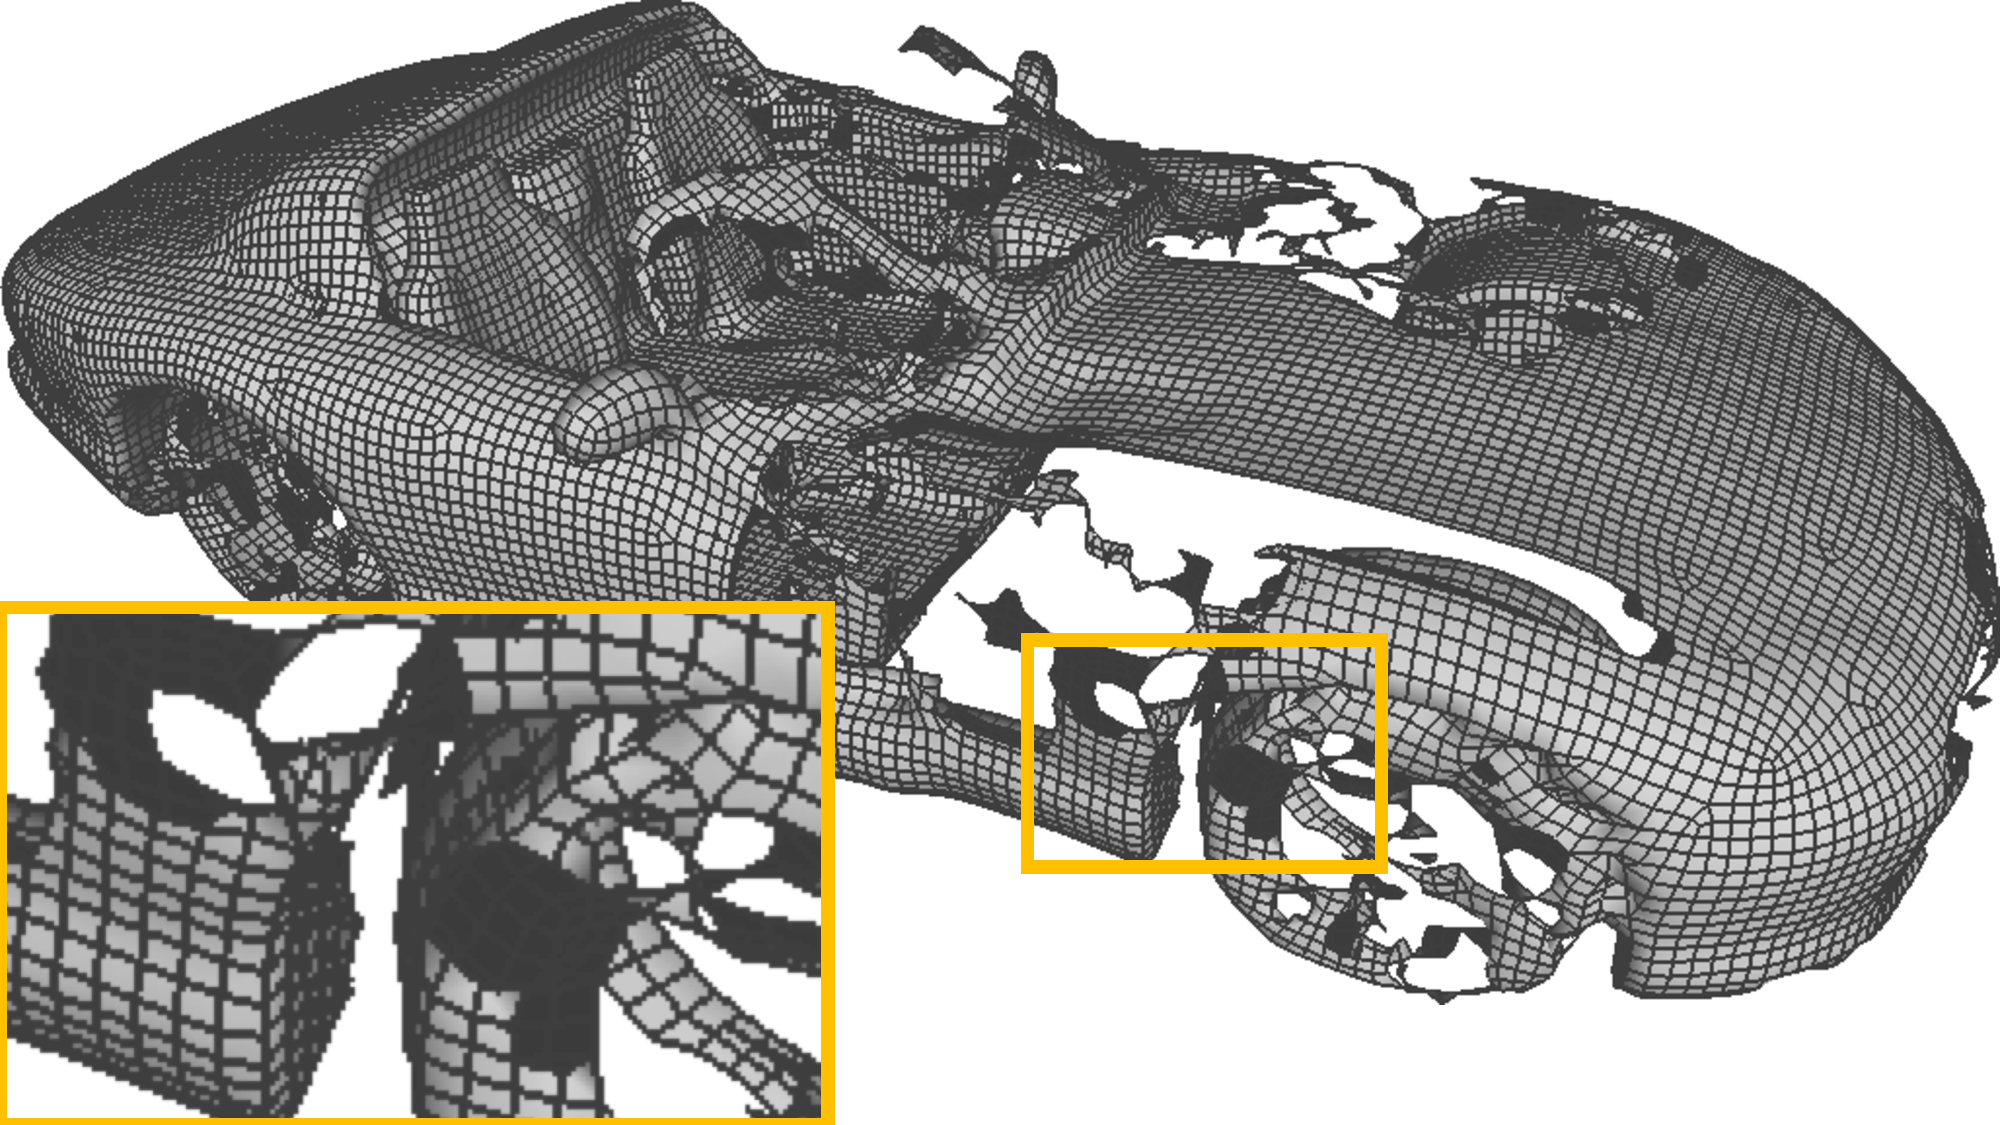
\includegraphics[width=\linewidth]{quadriflow/result/mesh01.pdf}\\
(a) Instant Meshes
\end{minipage}
\begin{minipage}{0.49\linewidth}
\centering
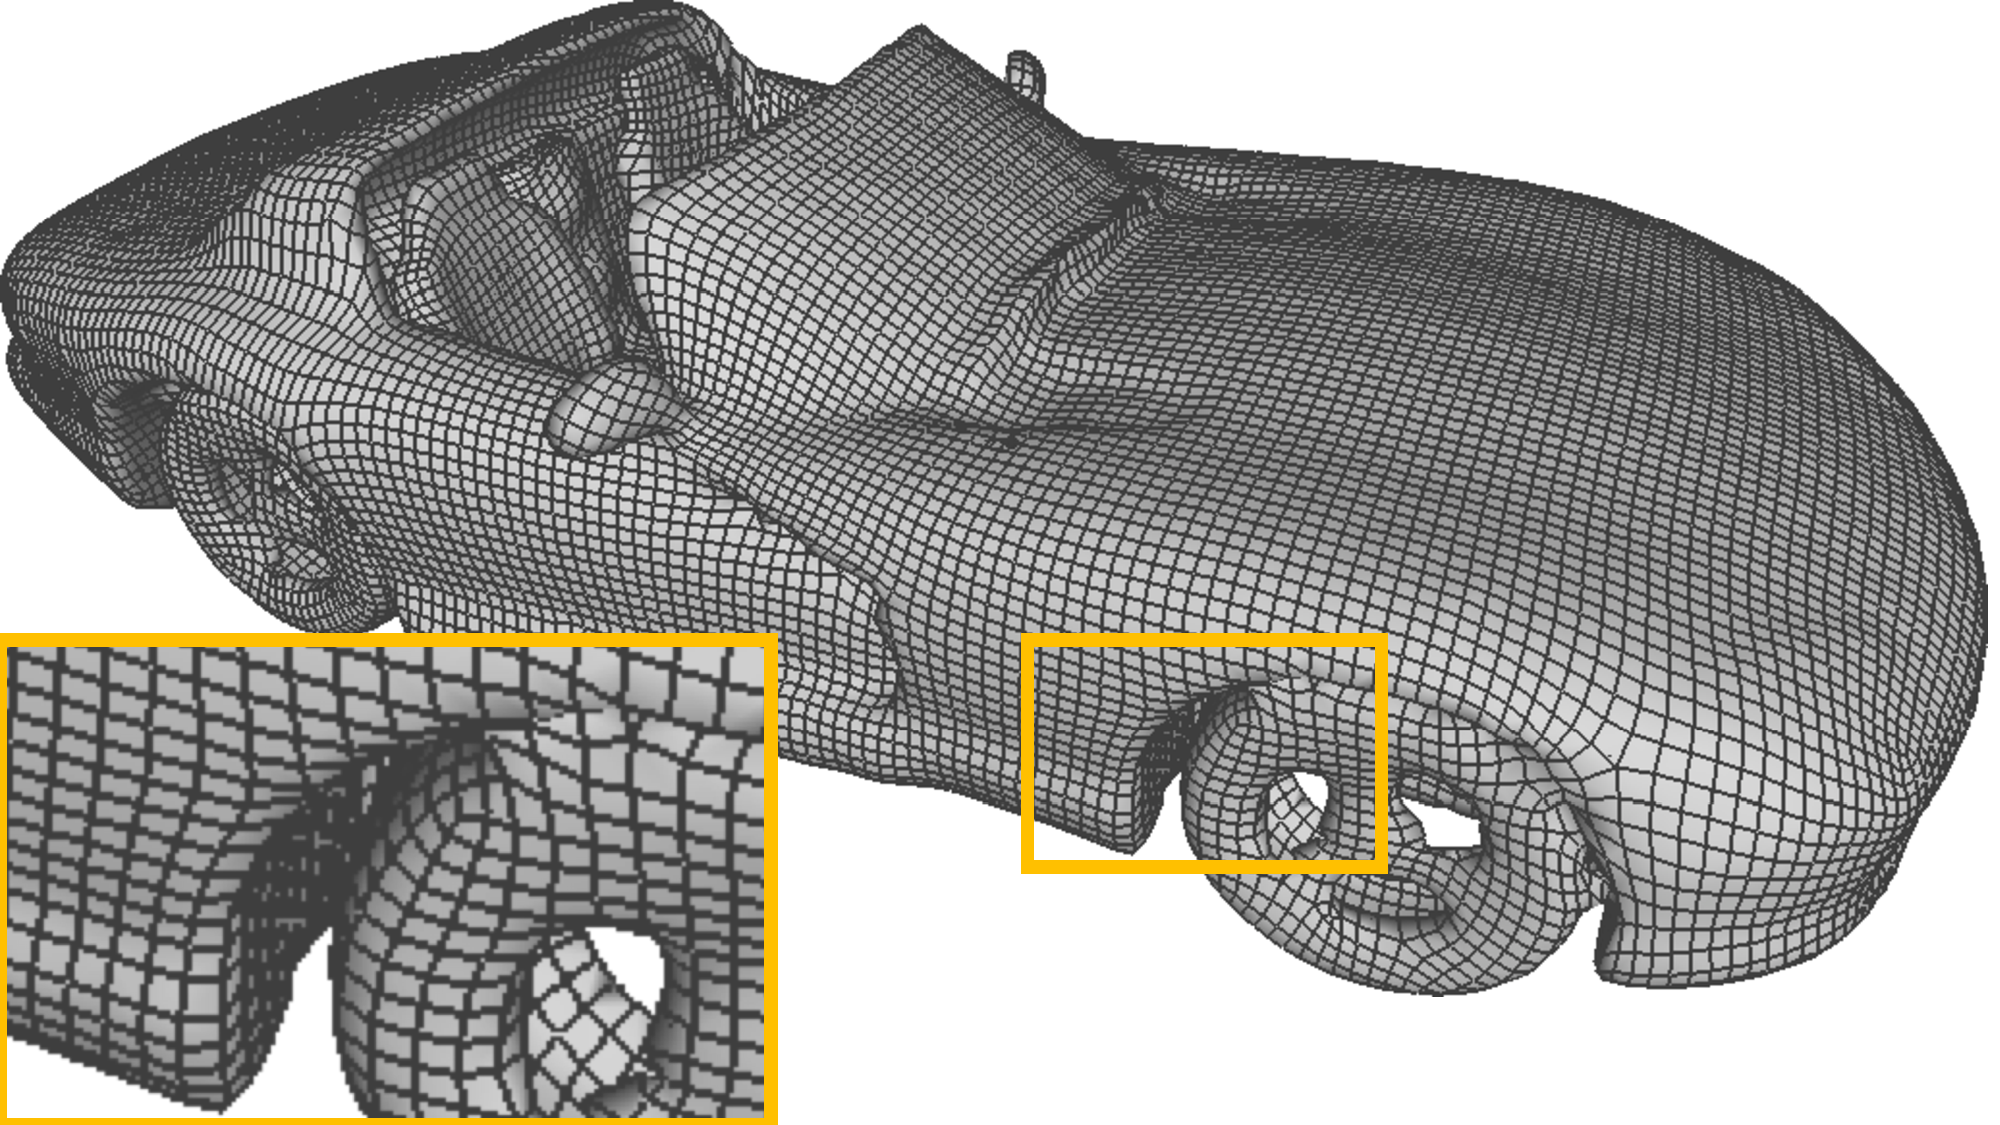
\includegraphics[width=\linewidth]{quadriflow/result/mesh00.pdf}\\
(b) QuadriFlow
\end{minipage}

\caption{(a) Example where a nonmanifold input triangulation leads to an Instant Mesh with holes. (b) Because QuadriMesh removes inverted triangles from the position field representation, it produces a manifold mesh with the correct topology.}
\label{fig:quad-fail-face}
\end{figure}


\section{Evaluation}
\label{sec:quad-evaluate}
Here we evaluate the quality, efficiency, and robustness of our method. We compare our mesh quality with prior methods; we thank the creators of those methods for sharing their meshes with us. We also compare implementations of several methods on 110 challenging car geometries from ShapeNet \cite{chang2015shapenet,huang2018robust}.
%%% JRS: I don't understand the following sentence. Also, it's awkward and unnecessary.
% We first evaluate the influence of several approximations and discuss their limitations. 

\subsection{Mesh Quality}

We compare our meshes with meshes generated by several other state-of-the-art methods. Table~\ref{tab:quad-statistics} lists the names of the models and properties related to the quality of the quad mesh: angle distortion (angle), area distortion (area), and the number of singularities (sings). The best numbers are in boldface.

\begin{table*}
\caption{Comparison of different methods. The best scores appear in boldface. QuadriFlow has slightly larger angle and area distortions than Instant Meshes, but it is usually better than the global methods MIQ and IGM. In terms of the number of singularities, QuadriFlow is competitive with these global methods, and it is significantly better than Instant Meshes.
% However, ours achieve the best for Buddha and Kitten100K.
\label{tab:quad-statistics}
}
\centering
\begin{tabular}{|c|r|r|r|c|r|r|r|}
\hline
Method & Angle & Area & Sings &
Method & Angle & Area & Sings \\
\hline
\multicolumn{4}{|c|}{David~\cite{alliez2003anisotropic}}  & \multicolumn{4}{c|}{Pig~\cite{alliez2003anisotropic}}  \\
\hline
Alliez et al. & 23.6 & 0.74 & 10310 & Alliez et al. & 17.7 & 0.61 & 436 \\
\hline
Instant Meshes & \textbf{10.9} & \textbf{0.22} & 2708 & Instant Meshes & \textbf{8.4} & 0.19 & 148 \\
\hline
QuadriFlow & 14.4 & 0.26 & \textbf{212} & QuadriFlow & 10.0 & \textbf{0.18} & \textbf{38} \\
\hline
\multicolumn{4}{|c|}{Fandisk~\cite{marinov2006robust}} & \multicolumn{4}{c|}{RockerArm~\cite{marinov2006robust}}  \\
\hline
Marinov \& Kobbelt & 18.0 & 0.63 & 59 & Marinov \& Kobbelt & 14.9 & 0.43 & 117 \\
\hline
Instant Meshes & \textbf{7.14} & \textbf{0.18} & 117 & Instant Meshes & \textbf{6.9} & \textbf{0.15} & 132 \\
\hline
QuadriFlow & 7.65 & 0.38 & \textbf{38} & QuadriFlow & 10.9 & 0.20 & \textbf{52} \\
\hline
\multicolumn{4}{|c|}{Bunny~\cite{tarini2010practical}} & \multicolumn{4}{c|}{Gargoyle~\cite{tarini2010practical}}  \\
\hline
Tarini et al. & 15.8 & 0.24 & 3438 & Tarini et al. & 17.4 & 0.23 & 4283 \\
\hline
Instant Meshes & \textbf{7.2} & \textbf{0.15} & 351 & Instant Meshes & \textbf{9.85} & \textbf{0.20} & 659 \\
\hline
QuadriFlow & 10.4 & 0.19 & \textbf{56} & QuadriFlow & 16.5 & 0.27 & \textbf{218} \\
\hline
\multicolumn{4}{|c|}{Omotondo~\cite{tarini2010practical}} & \multicolumn{4}{c|}{Rampant~\cite{tarini2010practical}}  \\
\hline
Tarini et al. & 17.4 & 0.24 & 3903 & Tarini et al. & 17.4 & 0.31 & 3745 \\
\hline
Instant Meshes & \textbf{7.8} & \textbf{0.17} & 367 & Instant Meshes & \textbf{8.3} & \textbf{0.18} & 455 \\
\hline
QuadriFlow & 14.3 & 0.23 & \textbf{80} & QuadriFlow & 12.2 & 0.23 & \textbf{158} \\
\hline
\multicolumn{4}{|c|}{Fandisk~\cite{bommes2009mixed}}  & \multicolumn{4}{c|}{Fertility~\cite{bommes2009mixed}}  \\
\hline
MIQ & 8.21 & 0.39 & \textbf{30} & MIQ & 8.59 & 0.26 & \textbf{48} \\
\hline
Instant Meshes & \textbf{7.14} & \textbf{0.20} & 68 & Instant Meshes & \textbf{7.09} & \textbf{0.15} & 256 \\
\hline
QuadriFlow & 7.65 & 0.22 & 38 & QuadriFlow & 7.78 & 0.16 & 70 \\
\hline
\multicolumn{4}{|c|}{RockerArm~\cite{bommes2009mixed}} & \multicolumn{4}{c|}{Buddha~\cite{bommes2013integer}}  \\
\hline
MIQ & \textbf{5.5} & 0.30 & \textbf{36} & IGM & 12.0 & 0.28 & 108 \\
\hline
Instant Meshes & 7.6 & 0.19 & 132 & Instant Meshes & \textbf{9.3} & \textbf{0.20} & 301 \\
\hline
QuadriFlow & 10.9 & \textbf{0.17} & 52 & QuadriFlow & 11.6 & 0.22 & \textbf{92} \\
\hline
\multicolumn{4}{|c|}{Fandisk~\cite{bommes2013integer}}  & \multicolumn{4}{c|}{Feline~\cite{bommes2013integer}}  \\
\hline
IGM & 11.3 & 0.40 & \textbf{30} & IGM & 17.7 & 0.44 & \textbf{110} \\
\hline
Instant Meshes & \textbf{7.14} & \textbf{0.20} & 117 & Instant Meshes & \textbf{8.11} & \textbf{0.18} & 592 \\
\hline
QuadriFlow & 7.65 & 0.22 & 38 & QuadriFlow & 18.0 & 0.42 & 158 \\
\hline
\multicolumn{4}{|c|}{Hand~\cite{bommes2013integer}}  & \multicolumn{4}{c|}{Kitten100K~\cite{bommes2013integer}}  \\
\hline
IGM & 8.5 & 0.46 & \textbf{40} & IGM & 7.84 & 0.48 & 63 \\
\hline
Instant Meshes & \textbf{6.46} & 0.23 & 43 & Instant Meshes & \textbf{6.87} & \textbf{0.16} & 127 \\
\hline
QuadriFlow & 7.4 & \textbf{0.22} & 42 & QuadriFlow & 8.43 & 0.19 & \textbf{32} \\
\hline
\multicolumn{4}{|c|}{Bunny~\cite{myles2014robust}} & \multicolumn{4}{c|}{Gargoyle~\cite{myles2014robust}}  \\
\hline
Myles et al. & 13.5 & 0.25 & \textbf{30} & Myles et al. & 10.7 & 0.33 & 328 \\
\hline
Instant Meshes & \textbf{7.2} & \textbf{0.15} & 351 & Instant Meshes & \textbf{9.85} & \textbf{0.20} & 659 \\
\hline
QuadriFlow & 10.4 & 0.19 & 56 & QuadriFlow & 16.5 & 0.27 & \textbf{218} \\
\hline
\multicolumn{4}{|c|}{Kitten100K~\cite{myles2014robust}}  & \multicolumn{4}{c|}{Pig~\cite{myles2014robust}}  \\
\hline
Myles et al. & 13.1 & 0.46 & 75 & Myles et al. & 14.0 & 0.25 & 55 \\
\hline
Instant Meshes & \textbf{6.87} & \textbf{0.16} & 127 & Instant Meshes & \textbf{8.4} & 0.19 & 148 \\
\hline
QuadriFlow & 8.43 & 0.19 & \textbf{32} & QuadriFlow & 10.0 & \textbf{0.18} & \textbf{38} \\
\hline
\end{tabular}
\end{table*}

\paragraph*{Angle Distortion} is measured as $\sqrt{\frac{1}{N}\sum_{i}(\theta_i-90^\circ)^2}$, where the sum is over all the angles in the mesh and $N$ is their number. Our meshes have less angle distortion than IGM~\cite{bommes2013integer} and are comparable with Instant Meshes. As Figure~\ref{fig:quad-angle-distortion} shows, the bottom of the Fandisk mesh produced by IGM has large distortion, while ours does not. Instant Meshes usually introduces many unnecessary singularities, especially for irregular shapes.

\begin{figure}
\centering
\begin{minipage}{0.32\linewidth}
\centering
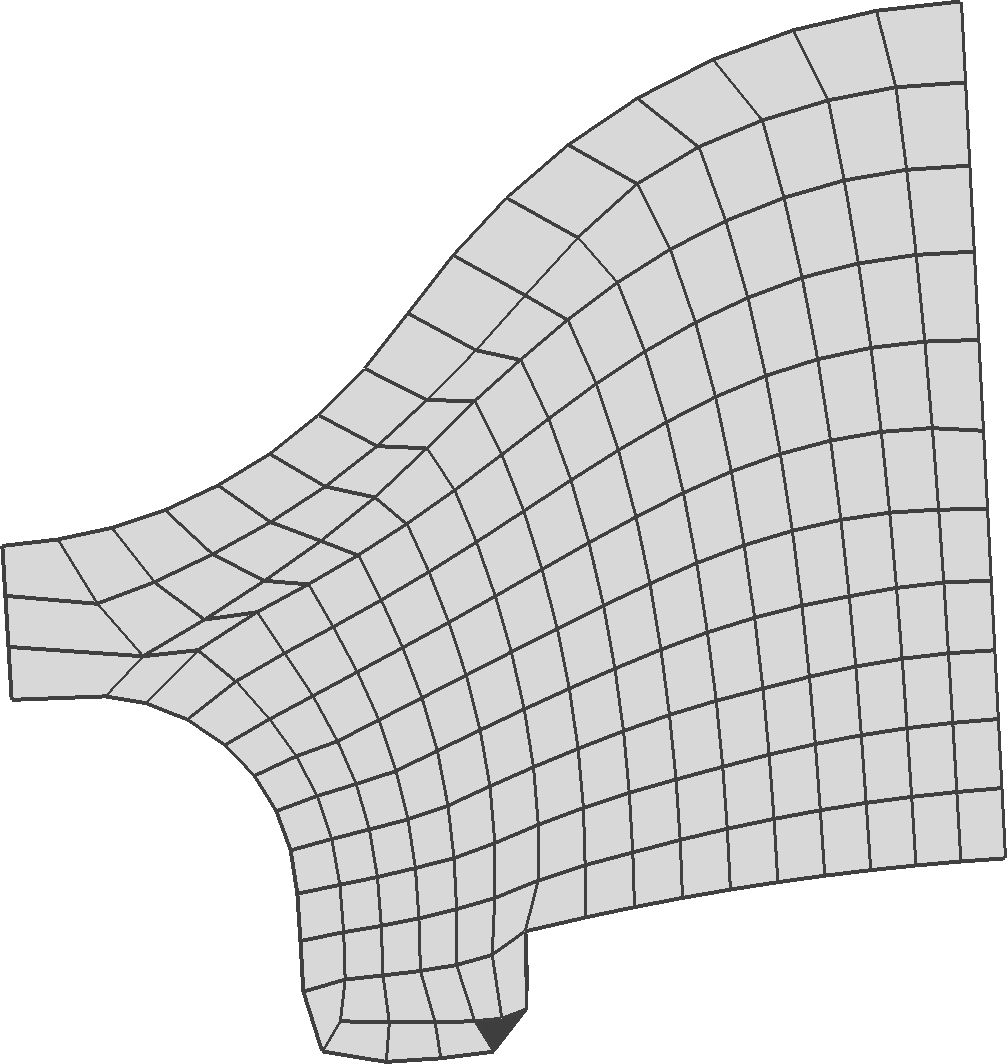
\includegraphics[width=\linewidth]{quadriflow/result/angle01.png}\\
(a) IGM\\
\end{minipage}
\begin{minipage}{0.32\linewidth}
\centering
\includegraphics[width=\linewidth]{quadriflow/result/angle02.png}\\
(b) Instant Meshes\\
\end{minipage}
\begin{minipage}{0.32\linewidth}
\centering
\includegraphics[width=\linewidth]{quadriflow/result/angle03.png}\\
(c) QuadriFlow
\end{minipage}

\caption{Quadrangulation of the model Fandisk using IGM, Instant Meshes, and QuadriFlow (our method). Our mesh has less angle distortion than IGM, and fewer vertices of irregular valence than Instant Meshes.}
\label{fig:quad-angle-distortion}
\end{figure}
\begin{figure}
     \centering
    \begin{minipage}{0.16\textwidth}
     \centering
   \includegraphics[width=\textwidth,height=1.33\textwidth]{quadriflow/result/area00.png}\\
   (a) Input triangulation
   \end{minipage}
    \begin{minipage}{0.16\textwidth}
     \centering
  \includegraphics[width=\textwidth,height=1.33\textwidth]{quadriflow/result/area01.png}\\
   (b) Integer-Grid Maps
   \end{minipage}
    \begin{minipage}{0.16\textwidth}
     \centering
  \includegraphics[width=\textwidth,height=1.33\textwidth]{quadriflow/result/area02.png}\\
   (c) Instant Meshes
   \end{minipage}
    \begin{minipage}{0.16\textwidth}
     \centering
  \includegraphics[width=\textwidth,height=1.33\textwidth]{quadriflow/result/area03.png}\\
   (d) QuadriFlow
   \end{minipage}
    \begin{minipage}{0.16\textwidth}
     \centering
  \includegraphics[width=\textwidth,height=1.33\textwidth]{quadriflow/teaser/teasers1.png}\\
   (e) QuadriFlow
   \end{minipage}
    \begin{minipage}{0.16\textwidth}
     \centering
  \includegraphics[width=\textwidth,height=1.33\textwidth]{quadriflow/teaser/teasers2.png}\\
   (f) QuadriFlow zoom
   \end{minipage}

\caption{Quadrilateral meshes generated by Integer-Grid Maps (IGM)~\cite{bommes2013integer}, Instant Meshes~\cite{jakob2015instant}, and our algorithm QuadriFlow. IGM~(b) sometimes produces badly distorted quadrilaterals. Instant Meshes~(c) produces more vertices of valence 3 or 5. QuadriFlow~(d,~e,~f) produces fewer vertices of irregular valence than Instant Meshes by removing all the singularities from the position field while producing less distortion than IGM.}
\label{fig:quad-teaser}
\end{figure}
\paragraph*{Area Distortion} is the standard deviation of the areas of the quadrilateral faces. As reported by Jakob et al., additional position singularities may alleviate distortion and improve the isotropy of the quad mesh. Our algorithm achieves comparable isotropy without additional position singularities, as Figure~\ref{fig:quad-teaser} shows.

Table~\ref{tab:quad-statistics} suggests that Mixed-Integer Quadrangulation (MIQ)~\cite{bommes2009mixed}, Integer-Grid Map (IGM)~\cite{bommes2013integer}, Instant Meshes~\cite{jakob2015instant}, and our QuadriFlow are the four best methods to discuss in detail. QuadriFlow meshes have slightly larger distortions than Instant Meshes, which is a reasonable price to pay for the dramatic reduction in the number of singularities---in practice, we are able to remove all the singularities from the position field. For the Buddha and Kitten100K models, QuadriFlow outperforms all other methods for singularities, but MIQ and IGM produce fewer singularities for other models.

The cross fields and resolutions of Instant Meshes and QuadriFlow meshes are exactly the same. The comparison meshes generated by other state-of-the-art methods used different cross fields and mesh resolutions. We subdivide their meshes to our resolution, followed by a Laplacian smoothing step. QuadriFlow meshes exhibit angle distortion similar to these methods, but it produces less area distortion, probably due to different cross fields or our MCF problem being easier to solve than the mixed-integer programming problems.  For all the models in Table~\ref{tab:quad-statistics}, QuadriFlow is able to generate an inversion-free integer offset ${\textbf{d}}^{\star}$ after enforcing the consistent orientation constraints. % Our quad generation method also guarantees no degenerate singularities. \jw{what is the best term for singularities with valance > 5?}.

% \paragraph*{Number of Singularities.}
Figure~\ref{fig:quad-singularity} plots the number of singularities in meshes of the Knot1 model (illustrated in Figure~\ref{fig:quad-shape-feature}) with respect to the target number of vertices. The blue bars count the number of orientation singularities for QuadriFlow, which produces no position singularities. The orange bars count the number of orientation singularities for Instant Meshes, and the green bars count the sum of orientation and position singularities for Instant Meshes. The number of position singularities in Instant Meshes increases linearly with the mesh density, which is one of its weaknesses.

\begin{figure}
\centering
\includegraphics[width=0.6\linewidth]{quadriflow/diagram/numsing.pdf}

\caption{Number of singularities in meshes of Knot1 as a function of the target number of vertices. Blue bars count the orientation singularities in QuadriFlow meshes; there are no position singularities. Orange bars count the orientation singularities in Instant Meshes, and green bars count their total orientation and position singularities.}
\label{fig:quad-singularity}
\end{figure}

% \paragraph*{Alignment to Shape Features.}
Because we use the extrinsic formulations from Instant Meshes, our mesh edges align with shape features better than IGM's, as Figure~\ref{fig:quad-shape-feature} shows.

\begin{figure}
\centering
\begin{minipage}{0.25\linewidth}
\centering
\includegraphics[width=\linewidth]{quadriflow/result/feature01.png}\\
(a) IGM\\
\end{minipage}
\begin{minipage}{0.25\linewidth}
\centering
\includegraphics[width=\linewidth]{quadriflow/result/feature02.png}\\
(b) Instant Meshes
\end{minipage}
\begin{minipage}{0.25\linewidth}
\centering
\includegraphics[width=\linewidth]{quadriflow/result/feature03.png}\\
(c) QuadriFlow
\end{minipage}

\caption{Surface quadrangulations of the model Knot1 using Integer-Grid Map (IGM), Instant Meshes, and QuadriFlow. As we borrow the extrinsic energy formulation from Instant Meshes, our mesh edges are aligned with shape features, unlike IGM's.}
\label{fig:quad-shape-feature}
\end{figure}

We compare Instant Meshes, Integer-Grid Map, and QuadriFlow in a subclass of ShapeNet with 110 challenging car models that the implementation of MIQ~\cite{bommes2009mixed} in \texttt{libigl} cannot handle. As before, the resolutions and the cross fields of the Instant Meshes and QuadriFlow meshes remain identical to each other, whereas we subdivide and smooth the Integer-Grid Map meshes to the same resolution. We do not have room to list all the models, so Table~\ref{tab:quad-car-compare} shows only the percentage of meshes for which QuadriFlow outperforms Instant Meshes or IGM according to the specified measurements. Note that there are models for which these two methods cannot produce reasonable meshes (see Section~\ref{quad-robustness}); though QuadriFlow can mesh all the models well, we omit from the comparison models for which one of the other methods produce conspicuous visual artifacts. Table~\ref{tab:quad-car-compare} indicates that QuadriFlow meshes exhibit less distortion than IGM, but more than Instant Meshes. For most models, we attain the minimum number of singularities. Figure~\ref{fig:quad-challenge} illustrates several of our meshes, with the models kindly supplied by Jakob et al.\ or ShapeNet.

\begin{table}
\caption{Comparisons tabulating the percentage of 110 ShapeNet car models for which QuadriFlow outperforms Integer-Grid Maps (IGM) or Instant Meshes based on the angle distortion, the area distortion, or the number of singularities. We exclude models on which IGM or Instant Meshes fails to produce a usable mesh. Instant Meshes have the least distortion, whereas QuadriFlow meshes have the fewest singularities.
\label{tab:quad-car-compare}
}

\centering
\begin{tabular}{|c|r|r|r|}
\hline
Method & Angle & Area & \# of sings \\
\hline
QuadriFlow vs.\ IGM & 59\% & 100\% & 97\% \\
\hline
QuadriFlow vs.\ Instant Meshes & 9\% & 5\% & 100\% \\
\hline
\end{tabular}
\end{table}


\begin{figure}
\centering
\includegraphics[width=0.6\linewidth]{quadriflow/diagram/timing.pdf}

\caption{QuadriFlow running times on the Hand model as a function of the number of faces of the input triangulation. (We subdivide the Hand model to the desired number of faces in advance.) We plot the initial Instant Meshes time, the time to enforce constraints, the time for post-processing, and the total time.}
\label{fig:quad-Timing}
\end{figure}
\subsection{Robustness}
\label{quad-robustness}

To test the robustness of our algorithm, we ran QuadriFlow on 17,791 watertight triangle manifolds generated by Huang, Su, and Guibas~\cite{huang2018robust} from the ShapeNet repository~\cite{chang2015shapenet}, as well as the models provided by Jakob et al.~\cite{jakob2015instant}. For every model, QuadriFlow always generates a manifold quadrilateral mesh and removes all the position singularities, and the chamfer distances to the original meshes are always less than 5\% of the average edge length in the quad mesh. This validates the robustness of our algorithm. We are able to preserve the watertightness of every model provided by Jakob et al., but not for about 20\% of the ShapeNet models, because the SAT algorithm cannot eliminate every inverted triangle. By contrast, MIQ~\cite{bommes2009mixed} as implemented in \texttt{libigl}~\cite{jacobson2013libigl} fails on most of these models.

Recall from Table~\ref{tab:quad-car-compare} that we tested Instant Meshes and IGM on 110 watertight car manifolds from ShapeNet. IGM can produce high-quality meshes for 62 of them. Instant Meshes is able to generate quad meshes for all of them, but 52 of those contain large holes. QuadriFlow succeeds on all of them. We provide the models and meshes in the supplementary material.

\subsection{Efficiency}

In Figure~\ref{fig:quad-Timing}, we chart running times of several stages of QuadriFlow as a function of the number of input triangular faces. The input is the Hand model from IGM~\cite{bommes2013integer}, subdivided to obtain a suitable number of faces. We implemented Instant Meshes using CUDA with a GTX 1070 GPU and ran our implementation on a 2.4 GHz CPU with a single thread. Our implementation has speed comparable to the fastest existing method~\cite{ebke2016interactively}, which runs on a decimated mesh and maps back to the original resolution. They report 5.7 seconds to mesh a model with 0.84 million faces, while directly processing it with a state-of-the-art global method~\cite{ebke2014level} takes 161 seconds. We take only 5 seconds to process 0.86 million faces, and 20 seconds for 2.43 million faces.

In our experiments, the cost of MIQ~\cite{bommes2009mixed} as implemented in \texttt{libigl} varies a lot for different models. It takes over two minutes to process 14,000 faces, and more than two hours for 100,000 faces for the Gargoyle model~\cite{tarini2010practical}. On our 110-car dataset, IGM takes 50 to 600 seconds to process each model, while our method meshes each model in at most 10 seconds.

\subsection{Methodology}
\label{sec:quad-methodology}

Recall that our algorithm introduces an ILP approximation of a MIP problem, then formulates it as an MCF problem, which is also approximate because of the need to fix some integer offsets to balance the variables. Here we evaluate the influence of these approximations on the mesh quality.

\paragraph*{ILP Approximation.} Instead of jointly optimizing the continuous energy and integer constraints with MIP, we approximate the MIP problem with an ILP problem. Because we do not directly optimize the energy, the ILP solution might not obtain the best energy. This can cause a loss of geometric details when the mesh is coarse. Figure~\ref{fig:quad-coarse} shows the QuadriFlow meshes for the Hand model with different choices of mesh density. At the coarsest resolution, QuadriFlow loses four fingers.

\begin{figure}
\centering
\begin{minipage}{0.24\linewidth}
\centering
\includegraphics[width=\linewidth]{quadriflow/evaluation/coarse01.png}
131 vertices
\end{minipage}
\begin{minipage}{0.24\linewidth}
\centering
\includegraphics[width=\linewidth]{quadriflow/evaluation/coarse02.png}
344 vertices
\end{minipage}
\begin{minipage}{0.24\linewidth}
\centering
\includegraphics[width=\linewidth]{quadriflow/evaluation/coarse03.png}
1486 vertices
\end{minipage}
\begin{minipage}{0.24\linewidth}
\centering
\includegraphics[width=\linewidth]{quadriflow/evaluation/coarse04.png}
3365 vertices
\end{minipage}
\caption{A limitation of our method for coarse mesh generation. As we approximate an MIP problem as a minimum cost flow problem, geometric details can be lost when the target mesh density is low.}
\label{fig:quad-coarse}
\end{figure}

\paragraph*{MCF Approximation.} To solve the ILP problem, we further approximate it as an MCF problem by fixing some integer offsets to balance the variables.  To test how such an approximation affects the mesh, we experimented on the Hand model with a target resolution of 3,365 vertices. We randomly picked ten different starting triangles for the BFS algorithm.  We find that the percentage of fixed variables ranges from 0.6\% to 0.7\%, which is small. The gap between the worst and the best angle distortion or area distortion is less than 2\% of the median score. Thus we judge the influence of the MCF approximation to be small and acceptable.

\begin{table}[tbp]
\centering
\caption{Comparison of multiple methods for integer optimization. We show the running times, average angle distortions, and average area distortions on two test examples.  The number 900 or 1,500 represents the specified edge density. MF, MCF, MR, and ILP stand for maximum flow, minimum cost flow, multi-resolution, and integer linear programming, respectively.}
\label{tab:quad-methodology}
\begin{tabular}{lrrr}
\hline
Mesh \& Algorithm      & Time   & Angle error & Area error \\ \hline
Hand\_900\_MF          & 0.85  & \textbf{11.195277}   & 0.272820    \\
Hand\_900\_MF\_MR      & \textbf{0.09}  & 12.695140    & \textbf{0.237884}   \\
Hand\_900\_MCF         & 4.12  & 12.555485   & 0.294125   \\
Hand\_900\_MCF\_MR     & 0.11  & 13.011465   & 0.263241   \\
Hand\_900\_ILP         & 280.00 & 12.555485   & 0.294125   \\ \hline
Hand\_1500\_MF         & 1.76  & 9.387929    & \textbf{0.193454}   \\
Hand\_1500\_MF\_MR     & \textbf{1.05}  & 10.391423   & 0.205469   \\
Hand\_1500\_MCF        & 13.41 & \textbf{8.786778}    & 0.210081   \\
Hand\_1500\_MCF\_MR    & 1.09  & 8.982389    & 0.220997   \\
Hand\_1500\_ILP        & 164.00   & \textbf{8.786778}    & 0.210081  \\  \hline
%Fandisk\_1500\_MF      & 1.32  & 9.275963    & 0.210627   \\
%Fandisk\_1500\_MF\_MR  & \textbf{0.74}  & \textbf{7.924584}    & 0.225036   \\
%Fandisk\_1500\_MCF     & 7.21  & 8.875881    & 0.222538   \\
%Fandisk\_1500\_MCF\_MR & 0.82  & 8.134397    & \textbf{0.212998}   \\
%Fandisk\_1500\_ILP     & 811.00   & 8.875881    & 0.222538   \\ \hline
\end{tabular}
\end{table}

\paragraph*{Comparison of Integer Solvers.} To justify the effectiveness of our network flow formulation and our multi-resolution framework, we performed experiments with different integer optimization algorithms on two test examples. Their running times and distortion metrics appear in Table~\ref{tab:quad-methodology}. We tested five different algorithms. \texttt{MF} is the Boykov--Kolmogorov algorithm that solves the maximum flow problem. \texttt{MF\_MR} is a multi-resolution version of \texttt{MF}. \texttt{MCF} is the network simplex algorithm from the LEMON library, which solves the minimum cost flow problem. \texttt{MCF\_MR} is a multi-resolution version of \texttt{MCF}, in which we first solve the lowest resolution with the network simplex algorithm, and then solve the highest resolution with \texttt{MF\_MR}. Lastly, \texttt{ILP} uses Gurobi Optimization~\cite{gurobi} to solve Equation~\eqref{eq:quad-formulation} as an integer linear program.

From the table, we see that multi-resolution can greatly shorten the running times. Furthermore, the network flow algorithms are far more efficient and stable than the integer linear programming algorithms provided by Gurobi, as the former are more specialized whereas ILP is NP-hard. To our surprise, maximum flow algorithms perform nearly as well as minimum cost flow algorithms as measured by the distortion metrics.  Perhaps this is because many maximum flow algorithms operate by repeatedly finding the shortest augmenting path, which tends to keep the $L_1$ norm of Expression~\eqref{eq:quad-formulation} small.

\begin{figure}
\centering
\includegraphics[width=0.32\linewidth]{quadriflow/result/result00.png}
\includegraphics[width=0.32\linewidth]{quadriflow/result/result01.png}
\includegraphics[width=0.32\linewidth]{quadriflow/result/result02.png}
\includegraphics[width=0.32\linewidth]{quadriflow/result/result03.png}
\includegraphics[width=0.32\linewidth]{quadriflow/result/result04.png}
\includegraphics[width=0.32\linewidth]{quadriflow/result/result05.png}
%\includegraphics[width=0.32\linewidth]{result/result06.png}
\includegraphics[width=0.32\linewidth]{quadriflow/result/result07.png}
\includegraphics[width=0.32\linewidth]{quadriflow/result/result08.png}
%\includegraphics[width=0.32\linewidth]{result/result09.png}
%\includegraphics[width=0.32\linewidth]{result/result10.png}
\includegraphics[width=0.32\linewidth]{quadriflow/result/result11.png}
\caption{More meshes generated by QuadriFlow. We thank Jakob et al.~\cite{jakob2015instant} and ShapeNet \cite{chang2015shapenet,huang2018robust} for providing the models.}
\label{fig:quad-challenge}
\end{figure}


\chapter{Texture Understanding}
\label{chapter:texturenet}
In this chapter, we discuss semantics and canonical space understanding from textured 3D surface or captured images. We discuss the semantic understanding in Section~\ref{sec:texturenet}, and the surface parameterization understanding in Section~\ref{sec:framenet}.

\section{TextureNet: Semantics from Texture}
\label{sec:texturenet}
\subsection{Introduction}
We propose a new convolutional neural network, \emph{TextureNet}~\cite{huang2018texturenet}, with a 2D convolution kernel that extracts features directly from high-resolution signals associated with 3D surface meshes.  Given a map that associates high-resolution signals with a 3D mesh surface (e.g., RGB photographic texture), we define convolutional filters that operate on those signals within domains defined by geodesic surface neighborhoods.   This approach combines the advantages of feature extraction from high-resolution signals (as in \cite{dai20183dmv}) with the advantages of view-independent convolution on 3D surface domains (as in \cite{tatarchenko2018tangent}).

During our investigation of this approach, we had to address several research issues, the most significant of which is how to define geodesic neighborhoods of a mesh.   One approach could be to compute a global UV parameterization for the entire surface and then define convolutional operators directly in UV space; however, that approach may induce significant deformations due to flattening, not always follow surface features, and/or produce seams at surface cuts.  Another approach could be to compute UV parameterizations for local neighborhoods independently; however, then adjacent neighborhoods might not be oriented consistently, reducing the ability of a network to properly learn orientation-dependent features.   Instead, we compute a 4-RoSy (four-fold rotationally symmetric) field on the surface using QuadriFlow~\cite{huang2018quadriflow} and define a new 4-RoSy convolutional operator that explicitly accounts for the 4-fold rotational ambiguity of the cross-field parameterization. A 4-RoSy (four-way rotationally symmetric) field is a configuration of 4 orthogonal tangent directions associated with each vertex in the shape of a cross that varies smoothly over the mesh surface.  Since the 4-RoSy field from QuadriFlow has no seams, aligns to shape features, induces relatively little distortion, has few singularities, and consistently orients adjacent neighborhoods (up to 4-way rotations), it provides an attractive trade-off between distortion and orientation invariance.

Results on 3D semantic segmentation benchmarks show an improvement of the 4-RoSy convolution on surfaces over alternative geometry-only approaches (by 6.4\%), plus significantly further improvement when applied to high-resolution color signals (by 6.9-8.2\% ).  With ablation studies, we verify the importance of the consistent orientation of a 4-RoSy field and demonstrate that our sampling and convolution operator works better than other alternatives.

\subsection{Related Work}
\label{related:texturenet}
\paragraph*{3D Deep Learning.}
With the availability of 3D shape databases \cite{wu20153d,chang2015shapenet,song2017semantic} and real-world labeled 3D scanning data \cite{song2015sun,armeni2017joint,dai2017scannet,chang2017matterport3d}, there is significant interest in deep learning on three-dimensional data.   Early work developed CNNs operating on 3D volumetric grids \cite{wu20153d,maturana2015voxnet}.  They have been used for 3D shape classification  \cite{qi2016volumetric,riegler2017octnet}, semantic  segmentation \cite{dai2017scannet,dai2018scancomplete}, object completion \cite{dai2017shape}, and scene completion \cite{dai2018scancomplete}.   More recently, researchers have developed methods that can take a 3D point cloud as input to a neural network and predict object classes or semantic point labels \cite{qi2017pointnet,qi2017pointnet++,tatarchenko2018tangent,su2018splatnet,atzmon2018point}.  AtlasNet~\cite{groueix2018papier} learns to generate surfaces of the 3D shape.  In our work, we utilize a sparse point sampled data representation, however, we exploit high resolution signals on geometric surface structures with a new 4-RoSy surface convolution kernel.

\paragraph*{Convolutions on Meshes.}
Several researchers have proposed methods for applying convolutional neural networks intrinsically on manifold meshes.  FeaStNet~\cite{verma2018feastnet} proposes a graph operator that establishes correspondences between filter weights. Jiang \textit{et al.}~\cite{jiang2019spherical} applies differential operators on unstructured spherical grids.
GCNN~\cite{masci2015geodesic} proposes using discrete patch operators on tangent planes parameterized by radius and angles. 
However, the orientation of their selected geodesic patches is arbitrary, and the parameterization is highly distorted or inconsistent at regions with high Gaussian curvature. 
ACNN~\cite{boscaini2016learning} observes this limitation and introduces the anisotropic heat kernels derived from principal curvatures. MoNet~\cite{monti2017geometric} further generalizes the architecture with the learnable gaussian kernels for convolutions.
The principal curvature based frame selection method is adopted by Xu \textit{et al.}~\cite{xu2017directionally} for segmentation of nonrigid surfaces, by Tatarchenko \textit{et al.}~\cite{tatarchenko2018tangent} for semantic segmentation of point clouds, and by ADD~\cite{boscaini2016anisotropic} for shape correspondence in the spectral domain. 
It naturally removes orientation ambiguity but fails to consider frame inconsistency problem, which is critical when performing feature aggregation.  Its problems are particularly pronounced in indoor scenes (which often have many planar regions where principal curvatures are undetermined) and in real-world scans (which often have noisy and uneven sampling where consistent principal curvatures are difficult to predict).   In contrast, we define a 4-RoSy field that provides consistent orientations for neighboring convolution domains.

\paragraph*{Multi-view and 2D-3D Joint Learning.}
Other researchers have investigated how to incorporate features from RGB inputs to 3D deep networks.  The typical approach is to simply assign color values to voxels, points, or mesh vertices and treat them as additional feature channels.
However, given that geometry and RGB data are at vastly different resolutions, this approach leads to significant downsampling of the color signal and thus does not take full advantage of the high-frequency patterns therein.   An alternative approach is to combine features extracted from RGB images in a multi-view CNN \cite{su2015multi}. This approach has been used for 3D semantic segmentation in 3DMV \cite{dai20183dmv}, where features are extracted from 2D RGB images and then back-projected into a 3D voxel grid where they are merged and further processed with 3D voxel convolutions.  Like our approach, 3DMV processes high-resolution RGB signals; however it convolves them in a 2D image plane, where occlusions and background clutter are confounding.  In contrast, our method directly convolves high-resolution signals intrinsically on the 3D surface which is view-independent.


\subsection{The TextureNet Approach}
Our approach performs convolutions on high-resolution signals with geodesic convolutions directly on 3D surface meshes.
The input is a 3D mesh associated with a high-resolution surface signal (e.g., a color texture map), and the outputs are learned features for a dense set of sample points that can be used for semantic segmentation and other tasks.   

Our main contribution is defining a smooth, consistently oriented domain for surface convolutions based on four-way rotationally symmetric (4-RoSy) fields.   We observe that 3D surfaces can be mapped with low-distortion to two-dimensional parameterizations anchored at dense sample points with locally consistent orientations and few singularities if we allow for a four-way ambiguity in the orientation at the sample points.   We leverage that observation in TextureNet by computing a 4-RoSy field and point sampling using QuadriFlow~\cite{huang2018quadriflow} and then building a network using new 4-RoSy convolutional filters (TextureConv) that are invariant to the four-way rotational ambiguity.   

\begin{figure}
\includegraphics[width=\linewidth]{texturenet/diagram/network.pdf}
\caption{TextureNet architecture. We propose a UNet~\cite{ronneberger2015u} architecture for hierarchical feature extraction. The key innovation in the architecture is the texture convolution layer. We efficiently query the local geodesic patch for each surface point, associating each neighborhood with a local, orientation-consistent texture coordinate system. This allows us to extract the local 3D surface features as well as high-resolution signals such as associated RGB input.}
\label{fig:texturenet-approach-network}
\end{figure}

We utilize this network design to learn and extract features from high-resolution signals on surfaces by extracting surface patches with high-resolution signals oriented by the 4-RoSy field at each sample point.   The surface patches are convolved by a few TextureConv layers, pooled at sample points, and then convolved further with TextureConv layers in a UNet~\cite{ronneberger2015u} architecture, as shown in Figure~\ref{fig:texturenet-approach-network}.  For down-sampling and up-sampling, we use the furthest point sampling and three-nearest neighbor interpolation method proposed by PointNet++~\cite{qi2017pointnet++}.  The output of the network is a set of features associated with point samples that can be used for classification and other tasks.   The following sections describe the main components of the network in detail.


\subsubsection{High-Resolution Signal Representation}
\label{sec:texturenet-high-res}
Our network takes as input a high-resolution signal associated with a 3D surface mesh. In the first steps of processing, it generates a set of sample points on the mesh and defines a parameterized high-resolution patch for each sample (Section \ref{sec:texturenet-approach-param}) \jw{as follows}: For each sample point $\mathbf{p}_i$, we first compute its geodesic neighborhood $\Omega_{\rho}(\mathbf{p}_i)$ (\jw{Eq.}~\ref{eq:texturenet-omega}) with radius $\rho$. Then, we sample an NxN point cloud $\{\mathbf{q}_{xy}|-N/2\leq x,y<N/2\}$. The texture coordinates for $\mathbf{q}_{xy}$ are $((x+0.5)d,(y+0.5)d)$ -- $d$ is the distance between the adjacent pixels in the texture patch. In practice, we select $N=10$ and $d=4$mm. Finally, we use our newly proposed ``TextureConv'' and max-pooling operators (Section \ref{sec:texturenet-approach-conv}) to extract the high-res feature $\mathbf{f}_i$ for each point $\mathbf{p}_i$.  


\subsubsection{4-RoSy Surface parameterization}
\label{sec:texturenet-approach-param}
 A critical aspect of our network is to define a consistently-oriented geodesic surface parameterization for any position on a 3D mesh. Starting with some basic definitions, for a sampled point $\mathbf{p}$ on the surface, we can locally parameterize its tangent plane by two orthogonal tangent vectors $\mathbf{i}$ and $\mathbf{j}$.  Also, for any point $\mathbf{q}$ on the surface, there exists a shortest path on the surface connecting $\mathbf{p}$ and $\mathbf{q}$, e.g., the orange path in Figure~\ref{fig:texturenet-geodesic}(a). By unfolding it to the tangent plane, we can map $\mathbf{q}$ along the shortest path to $\mathbf{q^*}$.   Using these constructs, we define the local texture coordinate $\mathbf{q}$ in $\mathbf{p}$'s neighborhood as
 \begin{equation*}
     \mathbf{t}_{\mathbf{p}}(\mathbf{q}) = \begin{bmatrix}
     \mathbf{i}^T & \mathbf{j}^T
     \end{bmatrix}(\mathbf{q}^*-\mathbf{p}).
 \end{equation*}
 We additionally define the local geodesic neighborhood of $\mathbf{p}$ with receptive field $\rho$ as
\begin{equation}
\Omega_\rho(\mathbf{p}) = \{\mathbf{q}\;|\;||\mathbf{t}_{\mathbf{p}}(\mathbf{q})||_\infty < \rho\}.
\label{eq:texturenet-omega}
\end{equation}
\begin{figure}
    \centering
    \includegraphics[width=\linewidth]{texturenet/geodesic/neighbor.pdf}
    \caption{(a) Local texture coordinates. (b) Visualization of geodesic neighborhoods $\Omega_\rho$ ($\rho$ = 20 cm) on a set of randomly sampled vertices.}
    \label{fig:texturenet-geodesic}
\end{figure}
 \begin{figure}
    \centering
     \includegraphics[width=\linewidth]{texturenet/param/param.pdf}
     \caption{(a) With an appropriate method like Quadriflow, we can get the surface parameterization aligned with shape features with negligible distortion. (b) Harmonic parameterization leads to high distortion in the scale. (c) Geometry images~\cite{gu2002geometry} result in high distortion in the orientation.}
     \label{fig:texturenet-param}
 \end{figure}
The selection for the set of mesh sampled positions $\{\mathbf{p}\}$ and their tangent vectors $\mathbf{i}$ and $\mathbf{j}$ is critical for the success of learning on a surface domain.  Ideally, we would select points whose spacing is uniform and whose tangent directions are consistently oriented at neighbors, such that the underlying parameterization has no distortions or seams, as shown in Figure~\ref{fig:texturenet-param}(a).  With those properties, we could learn convolutional operators with translation invariance exactly as we would for images.  Unfortunately, these properties are only achievable if the surface is a flat plane.   
For a general 3D surface, we can only hope to select a set of point samples and tangent vectors that minimize deviations between spacings of points and distortions of local surface parameterizations. Figure~\ref{fig:texturenet-param}(b) shows an example where harmonic surface parameterization introduces large-scale distortion -- a 2D convolution would include a large receptive field at the nose but a small one at the neck. Figure~\ref{fig:texturenet-param}(c) shows a geometry image~\cite{gu2002geometry} parameterization with high distortion in the orientation -- convolutions on such a map would have randomly distorted and irregular receptive fields, making it difficult for a network to learn canonical features.

Unfortunately, a smoothly varying direction field on the surface is usually hard to obtain. According to the study of the direction field design~\cite{ray2008n,lai2010metric}, the best-known approach to mitigate the distortion is to compute a four-way rotationally symmetric (\emph{4-RoSy}) \emph{orientation field}, which minimizes the deviation by incorporating directional ambiguity. Additionally, the orientation field needs a consistent definition among different geometries, and the most intuitive way is to make it align with the shape features like the principal curvatures. Fortunately, the extrinsic energy is used by \cite{jakob2015instant,huang2018quadriflow} to realize it. Therefore, we compute the extrinsic 4-Rosy orientation field at a uniform distribution of point samples using QuadriFlow~\cite{huang2018quadriflow} and use it to define the tangent vectors at any position on the surface. Because of the directional ambiguity, we randomly pick one direction from the cross as $\mathbf{i}$ and compute $\mathbf{j}=\mathbf{n}\times \mathbf{i}$ for any position. 

\begin{figure}
    \centering
    \includegraphics[width=\linewidth]{texturenet/diagram/wrap.pdf}
    \caption{Singularity at a cube vertex, (a)-(c) demonstrate three different ways of unfolding the local neighborhood. Such ambiguity is removed around the singularity by our texture coordinate definition using the shortest path. For the purple point, (a) is a valid neighborhood, while the blue points in (b) and orange points in (c) are unfolded along the paths which are not the shortest. Similarly, the ambiguity in the gap location is removed.}
    \label{fig:texturenet-wrap}
\end{figure}


Although there is a 4-way rotational ambiguity in this local parameterization of the surface (which will be addressed with a new convolutional operator in the next section), the resulting 4-RoSy field provides a way to extract geodesic neighborhoods consistently across the entire surface, even near singularities. 
Figure~\ref{fig:texturenet-wrap} (a,b,c) shows the ambiguity of possible unfolded neighborhoods at a singularity.  Since QuadriFlow~\cite{huang2018quadriflow} treats singularities as faces rather than vertices, all sampled positions have a well-defined orientation field. More importantly, the parameterization of every geodesic neighborhood is well-defined with our shortest path patch parameterization. For example, only Figure~\ref{fig:texturenet-wrap}(a) is a valid parameterization for the purple spot, while the location for the blue and orange spots in Figures~\ref{fig:texturenet-wrap}(b) and (c) are unfolded along the paths that are not the shortest. Unfolding a geodesic neighborhood around the singularity also causes another potential issue that a seam cut is usually required, leading to a gap at the 3-singularity or multiple-surface coverage at the 5-singularity. For example, there is a gap at the bottom-right corner in Figure~\ref{fig:texturenet-wrap}(a) caused by the seam cut shown as the green dot line. Fortunately, the location of the seam is also well-defined with our shortest-path definition: it must be the shortest geodesic path going through the singularity. Therefore, our definition of the local neighborhood guarantees a canonical way of surface parameterization even around corners and singularities.

\subsection{4-RoSy Surface Convolution Operator}
\label{sec:texturenet-approach-conv}
\begin{figure}
     \centering
     \begin{minipage}{0.32\linewidth}
     \centering
     \includegraphics[width=\linewidth,height=\linewidth]{texturenet/diagram/image_coordinate.pdf}\\
     \footnotesize{
     (a) Image Coordinate
     }
     \end{minipage}
     \begin{minipage}{0.32\linewidth}
     \centering
     \includegraphics[width=\linewidth,height=\linewidth]{texturenet/diagram/cube_coordinate.pdf}\\
     \footnotesize{
     (b) 3D parametrization
     }
     \end{minipage}
     \begin{minipage}{0.32\linewidth}
     \centering
     \includegraphics[width=\linewidth,height=\linewidth]{texturenet/diagram/conv_coordinate.pdf}\\
     \footnotesize{
     (c) Inconsistent Frame
     }
     \end{minipage}
     \caption{(a) Traditional convolution kernel on a regular grid. (b) Frames defined by the orientation field on a 3D cube. (c) For the patch highlighted in orange in (b), multi-layer feature aggregation would be problematic with traditional convolution due to the frame inconsistency caused by the directional ambiguity of the orientation field.}
     \label{fig:texturenet-singular}
 \end{figure}

TextureNet~is a network architecture composed of convolutional operators acting on geodesic neighborhoods of sample points with 4-RoSy parameterizations.
The input to each convolutional layer is three-fold: 1) a set of 3D sample points associated with features (e.g., RGB, normals, or features computed from high-resolution surface patches or previous layers); 2) a coordinate system stored as two tangent vectors representing the 4-RoSy cross-field for each point sample; and 3) a coarse triangle mesh, where each face is associated with the set of extracted sampled points and connectivity indices that support fast geodesic patch query and texture coordinate computation for the samples inside a geodesic neighborhood, much like the PTex~\cite{burley2008ptex} representation for textures. 

Our key contribution in this section is the design of a convolution operator suitable for 4-RoSy fields. 
The problem is that we cannot use traditional 3x3 convolution kernels on domains parameterized with 4-RoSy fields without inducing inconsistent feature aggregation at higher levels.  Figure~\ref{fig:texturenet-singular} demonstrates the problem for a simple example.  Figure~\ref{fig:texturenet-singular}(a) shows 3x3 convolution in a traditional flat domain. Figure~\ref{fig:texturenet-singular}(b) shows the frames defined by our 4-RoSy orientation field of the 3D cube where red spots represent the singularities. Although the cross-field in the orange patch is consistent under the 4-RoSy metric, the frames are not parallel when they are unfolded into a plane (Figure~\ref{fig:texturenet-singular}(c)). Aggregation of features inside such a patch is therefore problematic.

``TextureConv'' is our solution to remove the directional ambiguity. It consists of four layers (in Figure~\ref{fig:texturenet-approach-network}), including geodesic patch search, texture space grouping, convolution and aggregation. To extract the geodesic patch for each input point $\Omega_\rho(\mathbf{p})$, we use breadth-first search with the priority queue to extract the face set in the order of \jw{geodesic distance from face center to $\mathbf{p}$}. We estimate the texture coordinate at the face center as well as its local tangent coordinate system, recorded as $(\mathbf{t}_f,\mathbf{i}_f,\mathbf{j}_f)$. In order to expand the search tree from face $u$ to $v$, we can approximate the texture coordinate at the face center as $\mathbf{t}_{v} = \mathbf{t}_{u} + (\mathbf{i}_u,\mathbf{j}_u)^T (\mathbf{c}_v - \mathbf{c}_u)$, where $\mathbf{c}_f$ represents the center position of the face $f$. $\mathbf{i}_v$ and $\mathbf{j}_v$ can be computed by rotating the coordinate system around the shared edge from face $u$ to $v$. After having the face set inside the geodesic patch, we can find the sampled points set associated with these faces. We estimate the texture coordinate of every sampled point $\mathbf{q}$ associated with each face $f$ as $\mathbf{t}_\mathbf{p}(\mathbf{q})=\mathbf{t}_f+(\mathbf{i}_f,\mathbf{j}_f)^T(\mathbf{q} - \mathbf{c}_f)$. By testing $||\mathbf{t}_\mathbf{p}(\mathbf{q})||_\infty < \rho$, we can determine the sampled points inside the geodesic patch $\Omega_\rho(\mathbf{p})$.

The texture space grouping layer segments the local neighborhood into 3x3 patches in the texture space, each of which is a square with edge length as $2\rho/3$, as shown in Figure~\ref{fig:texturenet-approach-network} (after the ``grouping arrow''). We could directly borrow the image convolution method linearly transform each point feature with 9 different weights according to their belonging patch. However, we propose a 4-RoSy convolution kernel to deal with the directional ambiguity. As shown in Figure~\ref{fig:texturenet-approach-network}, all sampled points can be categorized as at the corners ($\{\mathbf{p}_j^1\}$), edges ($\{\mathbf{p}_j^2\}$) or the center ($\{\mathbf{p}_j^3\}$). Each sampled point feature is convolved with a 1x1 convolution as $h_1$, $h_2$ or $h_3$ based on its category. The extracted 4-rosy feature removes the ambiguity and allows higher-level feature aggregation. The \jw{channel-wise} aggregation operator $g$ can be max-pooling or average-pooling followed by the ReLu layer. In the task for semantic segmentation, we choose max-pooling since it is better at preserving salient signals.

\subsection{TextureNet Evaluation}

To investigate the performance of TextureNet, we ran a series of 3D semantic segmentation experiments for indoor scenes.   In all experiments, we train and test on the standard splits of the ScanNet~\cite{dai2017scannet} and Matterport3D~\cite{dai2017scannet} datasets.  Following previous works, we report mean class intersection-over-union (mIoU) results for ScanNet and mean class accuracy for Matterport3D.

%%%%%%%%%%%%%%%%%%%%%%%%%%%%%%%%%%%%%%%%%%%%
\para{Comparison to State-of-the-Art.}
\label{sec:texturenet-eval-result}

\begin{table*}
    \centering
    \scriptsize
    \tabcolsep=0.02cm
    \begin{tabular}{|c|c|c|c|c|c|c|c|c|c|c|c|c|c|c|c|c|c|c|c|c||c|}
        \hline
        Input & wall & floor & cab & bed & chair & sofa & table & door & wind & shf & pic & cntr & desk & curt & fridg & show & toil & sink & bath & other & avg\\
        \hline
        PN$^+$\cite{qi2017pointnet++} & 66.4 & 91.5 & 27.8 & 56.3 & 64.0 & 52.7 & 37.3 & 28.3 & 36.1 & 59.2 & 6.7 & 28.0 & 26.2 & 45.4 & 25.6 & 22.0 & 63.5 & 38.8 & 54.4 & 20.0 & 42.5\\
        \hline
        SplatNet\cite{su2018splatnet} & \textbf{69.9} & 92.5 & 31.1 & 51.1 & 65.6 & 51.0 & 38.3 & 19.7 & 26.7 & 60.6 & 0.0 & 24.5 & 32.8 & 40.5 & 0.0 & 24.9 & 59.3 & 27.1 & 47.2 & 22.7 & 39.3 \\
        \hline
        Tangent\cite{tatarchenko2018tangent} & 63.3 & 91.8 & 36.9 & 64.6 & 64.5 & 56.2 & 42.7 & 27.9 & 35.2 & 47.4 & 14.7 & 35.3 & 28.2 & 25.8 & 28.3 & 29.4 & 61.9 & 48.7 & 43.7 & 29.8 & 43.8\\
        \hline
        3DMV\cite{dai20183dmv} & 60.2 & 79.6 & 42.4 & 53.8 & 60.6 & 50.7 & 41.3 & 37.8 & 53.9 & 64.3 & 21.4 & 31.0 & 43.3 & 57.4 & \textbf{53.7} & 20.8 & 69.3 & 47.2 & 48.4 & 30.1 & 48.4\\
        \hline
        Ours & 68.0 & \textbf{93.5} & \textbf{49.4} & \textbf{66.4} & \textbf{71.9} & \textbf{63.6} & \textbf{46.4} & \textbf{39.6} & \textbf{56.8} & \textbf{67.1} & \textbf{22.5} & \textbf{44.5} & \textbf{41.1} & \textbf{67.8} & 41.2 & \textbf{53.5} & \textbf{79.4} & \textbf{56.5} & \textbf{67.2} & \textbf{35.6} & \textbf{56.6}\\
        \hline
    \end{tabular}\\
    (a) ScanNet (v2) (mean class IoU)
    \centering
    \tabcolsep=0.015cm
    \begin{tabular}{|c|c|c|c|c|c|c|c|c|c|c|c|c|c|c|c|c|c|c|c|c|c||c|}
        \hline
        Input & wall & floor & cab & bed & chair & sofa & table & door & wind & shf & pic & cntr & desk & curt & ceil & fridg & show & toil & sink & bath & other & avg\\
        \hline
        PN$^+$\cite{qi2017pointnet++} & 80.1 & 81.3 & 34.1 & 71.8 & 59.7 & 63.5 & \textbf{58.1} & 49.6 & 28.7 & 1.1 & 34.3 & 10.1 & 0.0 & 68.8 & 79.3 & 0.0 & 29.0 & 70.4 & 29.4 & 62.1 & 8.5 & 43.8 \\
        \hline
        SplatNet\cite{su2018splatnet} & \textbf{90.8} & \textbf{95.7} & 30.3 & 19.9 & \textbf{77.6} & 36.9 & 19.8 & 33.6 & 15.8 & 15.7 & 0.0 & 0.0 & 0.0 & 12.3 & 75.7 & 0.0 & 0.0 & 10.6 & 4.1 & 20.3 & 1.7 & 26.7 \\
        \hline
        Tangent\cite{tatarchenko2018tangent} & 56.0 & 87.7 & 41.5 & 73.6 & 60.7 & 69.3 & 38.1 & 55.0 & 30.7 & 33.9 & 50.6 & 38.5 & 19.7 & 48.0 & 45.1 & 22.6 & 35.9 & 50.7 & 49.3 & 56.4 & 16.6 & 46.8 \\
        \hline
        3DMV\cite{dai20183dmv} & 79.6 & 95.5 & \textbf{59.7} & 82.3 & 70.5 & \textbf{73.3} & 48.5 & 64.3 & 55.7 & 8.3 & 55.4 & 34.8 & 2.4 & \textbf{80.1} & \textbf{94.8} & 4.7 & 54.0 & 71.1 & 47.5 & 76.7 & 19.9 & 56.1 \\
        \hline
        Ours & 63.6 & 91.3 & 47.6 & \textbf{82.4} & 66.5 & 64.5 & 45.5 & \textbf{69.4} & \textbf{60.9} & \textbf{30.5} & \textbf{77.0} & \textbf{42.3} & \textbf{44.3} & 75.2 & 92.3 & \textbf{49.1} & \textbf{66.0} & \textbf{80.1} & \textbf{60.6} & \textbf{86.4} & \textbf{27.5} & \textbf{63.0} \\
        \hline
    \end{tabular}\\
    (b) Matterport3D (mean class accuracy)
    \caption{Comparison with the state-of-the-art methods for 3D semantic segmentation on the (a) ScanNet v2, and (b) Matterport3D~\cite{chang2017matterport3d} benchmarks. PN$^+$, SplatNet, and Tangent Convolution use points with per-point normal and color as input. 3DMV uses 2D images and voxels.  Ours uses grid points with high-res 10x10 texture patches.}
    \label{tab:texturenet-mainresult}
\end{table*}

\begin{figure*}
    \centering
    \includegraphics[width=\linewidth]{texturenet/result/scannet_horizontal.pdf}
    \caption{Visualization on ScanNet (v2)~\cite{dai2017scannet}. In the first row, we correctly predict the lamp, pillow, picture, and part of the cabinet, while other methods fail. In the second row, we predict the window and the trash bin correctly, while 3DMV~\cite{dai20183dmv} predicts part of the window as the trash bin and other methods fail.  The third row (zoom-in) highlights the differences.}
    \label{fig:texturenet-result-scannet}
\end{figure*}

\begin{figure}[t]
    \centering
    \begin{minipage}{0.32\linewidth}
    \centering
    \includegraphics[width=\linewidth]{texturenet/neighbors/gt.jpg}
    (a) Ground Truth
    \end{minipage}
    \begin{minipage}{0.32\linewidth}
    \centering
    \includegraphics[width=\linewidth]{texturenet/neighbors/pointnet.jpg}
    (b) Ball
    \end{minipage}
    \begin{minipage}{0.32\linewidth}
    \centering
    \includegraphics[width=\linewidth]{texturenet/neighbors/ours.jpg}
    (c) Ours
    \end{minipage}
    \caption{Visual results using different neighborhoods. With euclidean ball as a neighborhood, part of the table is predicted as the chair, since they belong to the same euclidean ball. This issue is solved by extracting features from the geodesic patches.}
    \label{fig:texturenet-neighbor}
\end{figure}

\begin{figure}[t]
    \centering
    \includegraphics[width=0.75\linewidth]{texturenet/result/matterport.pdf}
    \caption{Visual results on Matterport3D~\cite{chang2017matterport3d}. In all examples, our method is better at predicting the door, the toilet, the sink, the bathtub, and the curtain.}
    \label{fig:texturenet-result-Matterport3D}
\end{figure}

Our main result is a comparison of TextureNet to state-of-the-art methods for 3D semantic segmentation.  For this experiment, all methods utilize both color and geometry in their native formats.   Specifically, PointNet++~\cite{qi2017pointnet++}, Tangent Convolution~\cite{tatarchenko2018tangent}, SplatNet~\cite{su2018splatnet} use points with per-point normals and colors; 3DMV~\cite{dai20183dmv} uses 2D image features back-projected onto voxels; and Ours uses high-res 10x10 texture patches extracted from geodesic neighborhoods at sample points.

Table~\ref{tab:texturenet-mainresult} reports the mean IoU scores for all 20 classes of the ScanNet benchmark on the ScanNet (v2) and mean class accuracy on Matterport3D datasets.   They show that TextureNet (Ours) provides the best results on 18/20 classes for Scannet and 12/20 classes for Matterport3D.  Overall, the mean class IoU for Ours is 8.2\% higher than the previous state-of-the-art (3DMV) on ScanNet (48.4\% vs. 56.6\%), and our mean class accuracy is 6.9\% higher on Matterport3D (56.1\% vs. 63.0\%).  

Qualitative visual comparisons of the results shown in Figures~\ref{fig:texturenet-result-scannet}-\ref{fig:texturenet-result-Matterport3D} suggest that the differences between methods are often where high-resolution surface patterns are discriminating (e.g., the curtain and pillows in the top row of Figure~\ref{fig:texturenet-result-scannet}) and where geodesic neighborhoods are more informative than Euclidean ones (e.g., the lamp next to the bed).  Figure~\ref{fig:texturenet-neighbor} shows a case where convolutions with the geodesic neighborhoods clearly outperform their Euclidean counterparts. In Figure~\ref{fig:texturenet-neighbor}(b), part of the table is predicted as chair, probably because it is in a Euclidean ball covering nearby chairs. This problem is solved with our method based on geodesic patch neighborhoods. As shown in Figure~\ref{fig:texturenet-neighbor}(c), the table and the chairs are clearly segmented.

%%%%%%%%%%%%%%%%%%%%%%%%%%%%%%%%%%%%%%%%%%%%
\para{Effect of 4-RoSy Surface Parameterization.}

Our second experiment is designed to test how different surface parameterizations affect semantic segmentation performance -- i.e., how does the choice of the orientation field affect the learning process?   The simplest choice is to pick an arbitrary direction on the tangent plane as the x-axis, similar to GCNN~\cite{masci2015geodesic}, (Figure~\ref{fig:texturenet-coordinate}(a)).  A second option adopted by Tangent Convolution~\cite{tatarchenko2018tangent} considers a set of points $\mathbf{q}$ in a Euclidean ball centered at $\mathbf{p}$ and parameterizes the tangent plane by two eigenvectors corresponding to the largest two eigenvalues of the covariance matrix $\sum_{q}(p-q)(p-q)^T$.  A critical problem of this formulation is that the principal directions cannot be robustly analyzed at planar regions or noisy surfaces (Figure~\ref{fig:texturenet-coordinate}(b)). It also introduces inconsistency to the coordinate systems of the neighboring points, which vexes the feature aggregation at higher levels.  A third alternative is to use the intrinsic energy function~\cite{jakob2015instant} or other widely used direction field synthesis technique~\cite{ray2008n,lai2010metric}, which is not geometry-aware and therefore variant to 3D rigid transformation (Figure~\ref{fig:texturenet-coordinate}(c)). Our choice is to use the extrinsic energy to synthesize the direction field~\cite{huang2018quadriflow,jakob2015instant}, which is globally consistent and the only variant to geometry itself (Figure~\ref{fig:texturenet-coordinate}(d)).

\begin{figure}
    \centering
    \begin{minipage}{0.24\linewidth}
    \centering
    \includegraphics[width=\linewidth]{texturenet/field/random.jpg}
    (a) RandomVec
    \end{minipage}
    \begin{minipage}{0.24\linewidth}
    \centering
    \includegraphics[width=\linewidth]{texturenet/field/eigen.jpg}
    (b) EigenVec
    \end{minipage}
    \begin{minipage}{0.24\linewidth}
    \centering
    \includegraphics[width=\linewidth]{texturenet/field/intrinsic.jpg}
    (c) Intrinsic
    \end{minipage}
    \begin{minipage}{0.24\linewidth}
    \centering
    \includegraphics[width=\linewidth]{texturenet/field/extrinsic.jpg}
    (d) Extrinsic
    \end{minipage}
    \caption{Direction fields from different methods. (a) Random directions lead to inconsistent frames. (b) Eigenvectors suffer from the same issue at flat area. (c) Intrinsic-energy based orientation field does not align to the shape features. (d) Our extrinsic-based method generates consistent orientation fields aligned with surface features.}
    \label{fig:texturenet-coordinate}
\end{figure}

\begin{table*}
    \centering
    \scriptsize
    \tabcolsep=0.04cm
    \begin{tabular}{|c|c|c|c|c|c|c|c|c|c|c|c|c|c|c|c|c|c|c|c|c|c|c|}
        \hline
        Input & wall & floor & cab & bed & chair & sofa & table & door & wind & bkshf & pic & cntr & desk & curt & fridg & show & toil & sink & bath & other & ave\\
        \hline
        Random & 37.6 & \textbf{92.5} & 37.0 & 63.7 & 28.5 & 56.9 & 27.6 & 15.3 & 31.0 & 47.6 & 16.5 & 36.6 & \textbf{53.3} & \textbf{51.2} & 15.4 & 24.7 & 59.3 & 47.6 & 53.3 & 27.0 & 41.1 \\
        \hline
        Intrinsic & 47.4 & 91.9 & 35.3 & 62.5 & 55.8 & 44.8 & 37.5 & 29.8 & 40.5 & 40.9 & 16.7 & 41.5 & 39.9 & 42.1 & 20.4 & 24.3 & 85.6 & 44.5 & 58.3 & 29.5 & 44.4 \\
        \hline
        EigenVec & 45.3 & 79.0 & 32.2 & 53.4 & 59.8 & 40.4 & 32.2 & 28.8 & 40.5 & 43.4 & \textbf{17.8} & 39.5 & 32.7 & 40.6 & 22.5 & 25.0 & 82.4 & 48.1 & 54.8 & 32.6 & 42.5 \\
        \hline
        Extrinsic & \textbf{69.8} & 92.3 & \textbf{44.8} & \textbf{69.4} & \textbf{75.8} & \textbf{67.1} & \textbf{56.8} & \textbf{39.4} & \textbf{41.1} & \textbf{63.1} & 15.8 & \textbf{57.4} & 46.5 & 48.3 & \textbf{36.9} & \textbf{40.0} & \textbf{78.1} & \textbf{54.0} & \textbf{65.4} & \textbf{34.4} & \textbf{54.8} \\
        \hline
    \end{tabular}
    \caption{Mean IoU for different direction fields on ScanNet (v2). The input is a pointcloud with a normal and rgb color for each point. {\em Random} refers to randomly picking an arbitrary direction for each sampled point. {\em Intrinsic} refers to solving for a 4-rosy field with intrinsic energy. {\em EigenVec} refers to solving for a direction field with the principal curvature. {\em Extrinsic} is our method, which solves a 4-rosy field with extrinsic energy.}
    \label{tab:texturenet-direction}
\end{table*}

To test the impact of this choice, we compare all of these alternative direction fields to create the local neighborhood parameterizations for our architecture and compare the results of 3D semantic segmentation on ScanNet (v1) test set.  As shown in Table~\ref{tab:texturenet-direction}, the choice for the random direction field performs worst since it does not provide consistent parameterization. The tangent convolution suffers from the same issue but gets a better result since it aligns with the shape features.  The intrinsic parameterization aligns with the shape features but is not a canonical parameterization -- for example, different rigid transformations of the same shape lead to different parameterizations. The extrinsic energy provides a canonical and consistent surface parameterization.  As a result, the extrinsic 4-rosy orientation field achieves the best results.


%%%%%%%%%%%%%%%%%%%%%%%%%%%%%%%%%%%%%%%%%%%%
\begin{table*}
    \centering
    \scriptsize
    \tabcolsep=0.045cm
    \begin{tabular}{|c|c|c|c|c|c|c|c|c|c|c|c|c|c|c|c|c|c|c|c|c|c|}
        \hline
         Input & wall & floor & cab & bed & chair & sofa & table & door & wind & bkshf & pic & cntr & desk & curt & fridg & show & toil & sink & bath & other & ave\\
        \hline
         XYZ & 64.8 & 90.0 & 39.3 & 65.8 & 74.8 & 66.6 & 50.5 & 33.9 & 35.6 & 58.0 & 14.0 & 54.3 & 42.1 & 45.4 & 30.9 & 43.0 & 67.7 & 47.9 & 55.8 & 32.2 & 50.6 \\
        \hline
         NRGB & 69.8 & 92.3 & 44.8 & \textbf{69.4} & 75.8 & \textbf{67.1} & 56.8 & 39.4 & 41.1 & 63.1 & 15.8 & \textbf{57.4} & 46.5 & 48.3 & \textbf{36.9} & 40.0 & 78.1 & \textbf{54.0} & 65.4 & 34.4 & 54.8 \\
        \hline
         Highres & \textbf{75.0} & \textbf{94.4} & \textbf{46.8} & 67.3 & \textbf{78.1} & 64.0 & \textbf{63.5} & \textbf{44.8} & \textbf{46.0} & \textbf{71.3} & \textbf{21.1} & 44.4 & \textbf{47.5} & \textbf{52.5} & 35.2 & \textbf{51.3} & \textbf{80.3} & 51.7 & \textbf{67.6} & \textbf{40.2} & \textbf{58.1} \\
        \hline
    \end{tabular}
    \caption{Mean IoU for different color inputs on ScanNet (v2). {\em XYZ} represents our network using raw point input; i.e., geometry only. {\em NRGB} represents our network taking input as the sampled points with per-point normal and color. {\em Highres} represents our network taking per-point normal and the 10x10 surface texture patch for each sampled point.}
    \label{tab:texturenet-highres}
\end{table*}


%%%%%%%%%%%%%%%%%%%%%%%%%%%%%%%%%%%%%%%%%%%%
\para{Effect of 4-RoSy Surface Convolution.}

Our third experiment is designed to test how the choice for the surface convolution operator affects learning.  In Table~\ref{tab:texturenet-operator}, PN$^+$(A) and PN$^+$ represent PointNet++ with average and max pooling, respectively. GCNN$^1$ and GCNN are geodesic convolutional neural networks~\cite{masci2015geodesic} with $N_\rho=3,N_\theta=1$ and $N_\rho=N_\theta=3$ respectively. ACNN represents anisotropic convolutional neural networks~\cite{boscaini2016learning} with $N_\rho=3,N_\theta=1$. RoSy$^1$ means a 3x3 convolution along the direction of the 1-rosy orientation field. RoSy$^4$ picks an arbitrary direction from the cross in the 4-rosy field. RoSy$^4$(m) applies 3x3 convolution for each direction of the cross in the 4-rosy field, aggregated by max pooling. Ours(A) and Ours represent our method with average and max pooling aggregation.

We find that GCNN, ACNN and RoSy$^4$ produce the lowest IoUs because they suffer from the inconsistency of frames when features are aggregated.  GCNN$^1$ does not suffer from this issue since there is only a single bin in the angle dimension. RoSy$^4$(m) uses the max-pooling to canonicalize the feature extraction, which is independent of the orientation selection and produces better results than RoSy$^4$. RoSy$^1$ achieves a higher score by generating a more globally consistent orientation field with higher distortion. From this study, the combination of the 4-rosy orientation field and our TextureNet is the best option for the segmentation task among these methods. \jw{Since we precompute the local parametrization, our training efficiency is similar to GCNN.} %Please refer to Supplemental~\ref{appendix:4rosy} for the detailed performance with each class.

\begin{table}
    \centering
    \tabcolsep=0.03cm
    \begin{tabular}{|c|c|c|c|c|c|}
        \hline
         Input & PN$^+$(A) & PN$^+$ & GCNN$^1$ & GCNN & ACNN\\
         \hline
         Geometry & 32.6 & 43.5 & 48.7 & 24.6 & 29.7\\
         \hline
         NRGB & 38.1 & 48.2 & 49.6 & 27.0 & 32.4\\
         \hline
         \multicolumn{6}{c}{}\\
         \hline
         Input &  RoSy$^1$ & RoSy$^4$ & RoSy$^1$(m) & Ours(A) & Ours\\
         \hline
         Geometry & 37.8 & 30.8 & 40.3 & 38.0 & \textbf{50.6}\\
         \hline
         NRGB & 47.8 & 34.5 & 42.6 & 39.1 & \textbf{54.8}\\
         \hline
    \end{tabular}
    \caption{Mean Class IoU with different texture convolution operators on ScanNet (v2). The input is the pointcloud for the first row (Geometry) and the pointcloud associated with the normal and rgb signal for the second row (NRGB).}
    \label{tab:texturenet-operator}
\end{table}

%%%%%%%%%%%%%%%%%%%%%%%%%%%%%%%%%%%%%%%%%%%%
\para{Effect of High-Resolution Color.}

Our fourth experiment tests how much convolving with high-resolution surface colors affects semantic segmentation.   Table~\ref{tab:texturenet-highres} compares the performance of our network with uncolored sampled points (XYZ), sampled points with the per-point surface normal and color (NRGB), and with the per-point normal and the 10x10 color texture patch (Highres) as input.  \jw{According to Table~\ref{tab:texturenet-operator}, our network is already superior with only XYZ or additional NRGB because of the convolution operator.} We find that providing TextureNet with Highres colors improves the mean class IoU by 3.3\%.  As expected, the impact is stronger from some semantic classes than others -- e.g., the IoUs for the bookshelf and picture classes increase 63.1$\rightarrow$71.3\% and 15.8$\rightarrow$21.1\%, respectively. %\jw{We show an additional comparison to O-CNN~\cite{wang2017cnn} which enables high-resolution signals for voxels in Supplemental~\ref{appendix:ocnn}.}

%%%%%%%%%%%%%%%%%%%%%%%%%%%%%%%%%%%%%%%%%%
\para{Comparisons Using Only Surface Geometry.}

As a final experiment, we evaluate the value of the proposed 3D network for semantic segmentation of inputs with only surface geometry (without color).  During experiments on ScanNet, TextureNet achieves 50.6\% mIoU, which is 6.4\% better than the previous state-of-the-art.   In comparison, ScanNet~\cite{dai2017scannet} = 30.6\%, Tangent Convolution~\cite{tatarchenko2018tangent} = 40.9\%, PointNet++~\cite{qi2017pointnet++} = 43.5\%, and SplatNet~\cite{su2018splatnet} = 44.2\%.  %Detailed class IoU results are provided in Supplemental~\ref{appendix:geometry}.


\section{FrameNet: Frame Estimation from RGB Images}
\label{sec:framenet}
\subsection{Introduction}
we propose a novel image-to-3D task: dense 3D \cframe{} estimation from a single image. We have implemented an algorithm for this task in a supervised setting.   To acquire ``ground truth'' \cframe{}, we leverage data from RGB-D scanning datasets, like ScanNet~\cite{dai2017scannet}, which provide large sets of images posed within reconstructed 3D meshes.  
We compute \cframe{} on the meshes and render them to the RGB images to produce training data.  There are multiple choices for how to define the frames.  A simple approach would be to use Manhattan frames; however, they
reflect only the global scene orientation (figure~\ref{fig:vis-direction}(a)).   Instead, we compute locally consistent 4-RoSy \cframe{} that follow principal curvatures using the Quadriflow algorithm~\cite{huang2018quadriflow} (figure~\ref{fig:vis-direction}(b)).  We find that the surface tangent directions computed this way are consistent with image features and can be learned by a network from 2D data.

The \cframes{} are fundamental 3D properties of a scene, as they imply the canonical transformation that maps the 3D surface to the image plane.  They provide not only the surface normal but also canonical tangent directions and their projections onto the image plane.  We show that predicting all these directions jointly can improve surface normal estimation, local patch description using SIFT features~\cite{lowe2004distinctive}, and allow the insertion of novel objects with correct orientation in augmented reality applications.

Overall, the core contributions of the paper are:
     \vspace{-0.05in}
\begin{itemize}
     \item Identifying an important new 3D vision problem: local canonical frame estimation from RGB images.
    \vspace{-0.1in}
    \item Using projected tangent principal directions to improve \cframe{} estimation, outperforming existing works on surface normal estimation.
    \vspace{-0.1in}
    \item Exploiting tangent projected principal directions to compute perspective invariant feature descriptors.
    \vspace{-0.1in}
    \item Inserting new elements in the scene in a manner aware of perspective distortions, for augmented reality.
\end{itemize}
\begin{figure}
    \centering
    \includegraphics[width=\linewidth]{FrameNet/graph/illus.pdf}
    \vspace{-0.3in}
    \caption{We visualize the directions by picking random seed points and tracing along projected directions in the image. \cam{(a) and (b) show the Manhattan and projected principal directions in the same scene, respectively. (c) shows that projected principal directions usually follow the texture directions or object boundaries.}}
    \label{fig:vis-direction}
    \vspace{-0.1in}
\end{figure}

\subsection{Related Work}
\label{related:framenet}
\paragraph*{3D from Single Image:}
Estimating 2.5D geometry properties from a single image has become popular in recent years. Traditional methods aim at understanding low-level image information and geometry constraints. For example, Torralba \textit{et al.}~\cite{torralba2002depth} exploits the scene structure to estimate the absolute depth values. Saxena \textit{et al.}~\cite{saxena2006learning} uses hand-crafted features to predict the depth based on Markov random fields. Hoiem \textit{et al.}~\cite{hoiem2007recovering} recovers scene layout guided by the vanishing points and lines. Shi \textit{et al.}~\cite{shi2015break} estimates the defocus blur and uses it to assist depth estimation.

With the availability of large-scale datasets and the success of deep learning, many methods have been proposed for depth or/and normal estimation. For depth estimation, Eigen \textit{et al.}~\cite{eigen2014depth} uses CNN to predict indoor depth maps on the NYUv2 dataset. With the powerful backbone network like VGG~\cite{simonyan2014very} or ResNet~\cite{he2016deep}, depth estimation can be further improved~\cite{garg2016unsupervised,xie2016deep3d}. DORN~\cite{fu2018deep} proposes a novel ordinary loss and achieves the state-of-the-art in KITTI~\cite{geiger2013vision}. For surface normal estimation, Wang \textit{et al.}~\cite{wang2015designing} incorporate vanishing point and layout information in the network architecture. Eigen and Fergus~\cite{eigen2015predicting} trained a coarse-to-fine CNN to refine the details of the normals. The skip-connected architecture~\cite{bansal2016marr} is proposed to fuse hidden layers for normal estimation.

Since surface normal and depth are related to each other, another set of methods aimed at jointly predicting both to improve the performance. Wang \textit{et al.}~\cite{wang2016surge} exploits the consistency between normal and depth in planar regions. GeoNet~\cite{qi2018geonet} proposes a refinement network to enhance the depth and normal estimation from each other. Zhang \textit{et al.}~\cite{zhang2018deep} predict the normal and solve a global optimization problem to complete the depth.  We take a further step by jointly estimating all axes of a 3D canonical frame at each pixel, which helps both regularize the prediction through constraints and is useful in applications.

\paragraph*{Local Canonical Frames:}
\jw{Computing local \cframe{} on surfaces is a fundamental step for many problems.} 3DLite~\cite{huang20173dlite} builds \cframe{} in fitted 3D planes for color optimizations. GCNN~\cite{masci2015geodesic} defines local frames with spherical coordinates and applies discrete patch operators on tangent planes. ACNN~\cite{boscaini2016learning} introduces the anisotropic heat kernels derived from principal curvatures \jw{so that it can apply convolutions in canonical frames defined by principal axes. Such canonical frame} is also used in Xu \textit{et al.}~\cite{xu2017directionally} for nonrigid segmentation, by Tatarchenko \textit{et al.}~\cite{tatarchenko2018tangent,huang2018texturenet} for semantic segmentation of the 3D scenes. \jw{We aim at recognizing such frames from 2D images, and compute them from 3D surfaces to supervise the learning.}

TextureNet~\cite{huang2018texturenet} highlights the challenges of computing robust local \cframe{} at planar surface regions, where the principal curvatures are undetermined or highly influenced by noise or uneven sampling. Therefore, it proposes to compute a 4-RoSy orientation field to represent the principal directions. The 4-RoSy orientation field is an important concept in the geometry processing community~\cite{ray2008n,lai2010metric}. The target directions are aligned with the principal curvatures~\cite{cohen2003restricted,cazals2005estimating}, but regularized by additional energy to vary smoothly. This can be achieved by optimizing a nonlinear energy by periodic functions~\cite{hertzmann2000illustrating,ray2009geometry} or a mixed-integer representation~\cite{ray2008n,bommes2009mixed}. In our work, we use QuadriFlow~\cite{huang2018quadriflow} to optimize the 4-RoSy field so that it aligns with the principal curvatures at the curved surface and ensures smoothness in flat regions (where principal directions are ill-defined), as well as robustness to noise.

\subsection{Approach}
In this section, we develop our approach for learning local \cframe{} from RGB images. First, we discuss the ground truth labeling of \cframe{} from 2D images in Section~\ref{sec:framenet-prepare-data}. Then, we discuss the concept of projected tangent principal directions in Section~\ref{sec:framenet-project}. Finally in Section~\ref{sec:framenet-network}, we propose several energy terms that encourage the neural network to predict consistent local \cframe{} assisted by the projected tangent principal directions. Since we focus on the behavior of the local \cframe{} rather than the neural network architecture, we can adopt any neural network that predicts per-pixel features (see experiments in Sec. \ref{sec:framenet-evaluation} and \ref{sec:framenet-applications}).

\subsubsection{Local \ccff{} Generation}
\label{sec:framenet-prepare-data}
To label the \cframe, we need a dataset with 3D meshes aligned with RGB images to compute frames from geometry and render them to images as ground truth. We choose ScanNet~\cite{dai2017scannet} for our experiments.

\begin{figure}
    \centering
    \includegraphics[width=0.8\linewidth,height=0.584\linewidth]{FrameNet/graph/4rosy.pdf}
    \vspace{-0.20in}
    \caption{(a) computes the direction field from estimated principal curvatures. Noise exists in both the geometry and the projections in images, as shown in (c). (b) computes the 4-RoSy field using QuadriFlow~\cite{huang2018quadriflow} and produces robust tangent principal directions, as shown in (d) as the projection in the image plane.}
    \label{fig:framenet-vis-geometry}
\vspace{-0.1in}
\end{figure}

We compute \cframe{} as surface normals and tangent principal directions with the scene geometry. It is straightforward to compute surface normals, but tangent principal directions at flat regions are hard to compute especially in the presence of noise. As visualized in Figure~\ref{fig:framenet-vis-geometry}(a,c), the tangent principal directions can be pretty noisy. To solve this problem, we adopt the 4-RoSy field using QuadriFlow~\cite{huang2018quadriflow} as proposed by TextureNet~\cite{huang2018texturenet}, as shown in Figure~\ref{fig:framenet-vis-geometry}(b,d): This field generates consistent directions which vary smoothly at flatter regions and are aligned with the principal curvatures at curved surfaces. The cross-field is 4-RoSy since there are four valid choices for the tangent principal directions at each vertex. Considering this, we pick any pair of orthogonal tangent vectors in the cross-field to represent the principal directions, but we also view the other three alternatives as valid ground truth.

\begin{figure}
    \centering
     \begin{minipage}{0.19\linewidth}
     \centering
     \includegraphics[width=\linewidth]{FrameNet/Dataset/pred-000001-color.png}\\
     \includegraphics[width=\linewidth]{FrameNet/Dataset/pred-000003-color.png}\\
     %\includegraphics[width=\linewidth]{Dataset/pred-000005-color.png}\\
     \includegraphics[width=\linewidth]{FrameNet/Dataset/pred-000021-color.png}\\
     \vspace{-0.05in}
     RGB
    \end{minipage}
     \begin{minipage}{0.19\linewidth}
     \centering
     \includegraphics[width=\linewidth]{FrameNet/Dataset/pred-000001-X.png}\\
     \includegraphics[width=\linewidth]{FrameNet/Dataset/pred-000003-X.png}\\
     %\includegraphics[width=\linewidth]{Dataset/pred-000005-X.png}\\
     \includegraphics[width=\linewidth]{FrameNet/Dataset/pred-000021-X.png}\\
     \vspace{-0.05in}
     X
    \end{minipage}
     \begin{minipage}{0.19\linewidth}
     \centering
     \includegraphics[width=\linewidth]{FrameNet/Dataset/pred-000001-Y.png}\\
     \includegraphics[width=\linewidth]{FrameNet/Dataset/pred-000003-Y.png}\\
     %\includegraphics[width=\linewidth]{Dataset/pred-000005-Y.png}\\
     \includegraphics[width=\linewidth]{FrameNet/Dataset/pred-000021-Y.png}\\
     \vspace{-0.05in}
     Y
    \end{minipage}
     \begin{minipage}{0.19\linewidth}
     \centering
     \includegraphics[width=\linewidth]{FrameNet/Dataset/pred-000001-normal.png}\\
     \includegraphics[width=\linewidth]{FrameNet/Dataset/pred-000003-normal.png}\\
     %\includegraphics[width=\linewidth]{Dataset/pred-000005-normal.png}\\
     \includegraphics[width=\linewidth]{FrameNet/Dataset/pred-000021-normal.png}\\
     \vspace{-0.05in}
     Normal
    \end{minipage}
     \begin{minipage}{0.19\linewidth}
     \centering
     \includegraphics[width=\linewidth]{FrameNet/Dataset/pred-000001-vis-gt.png}\\
     \includegraphics[width=\linewidth]{FrameNet/Dataset/pred-000003-vis-gt.png}\\
     %\includegraphics[width=\linewidth]{Dataset/pred-000005-vis-gt.png}\\
     \includegraphics[width=\linewidth]{FrameNet/Dataset/pred-000021-vis-gt.png}\\
     \vspace{-0.05in}
     Projection
    \end{minipage}
    \caption{Local \ccff{} Dataset. For each RGB frame, we render the corresponding tangent principal directions (X and Y) for each pixel. The surface normal can be computed as the cross product of the principal directions.}
    \label{fig:framenet-dataset}
\vspace{-0.1in}
\end{figure}

We store the computed local \cframe{} on top of mesh vertices and render them to images after transforming them into the camera space. For each triangle to be rendered, we enumerate the $90^{\circ}N (N\in \mathbb{Z})$ degree rotations to the tangent principal directions of the last two vertices, so as to align them with the first vertex before the standard rasterization stage. This is to deal with the 4-way rotational ambiguities in the cross-field. For each RGB image, we render and save the tangent principal directions as two images, as shown in Figure~\ref{fig:framenet-dataset} as X and Y. The ground truth normal can be directly computed as the cross product of them.

\subsubsection{Projected Principal Directions}
\label{sec:framenet-project}
Since we aim to predict 3D principal tangent directions from their appearances into RGB images, we first derive the projective geometry that relates them.

%We observe that the projected tangent principal directions are mostly consistent with the object boundaries or image gradients as shown in Figure~\ref{fig:framenet-vis-geometry}(d). Therefore, we want to study the relationship between the tangent principal directions and their projections in the image.

 For a pixel $\mb{p}=(p_x,p_y)$ in the canonical camera coordinate system, its 3D position of the pixel can be represented as $\mb{P}=(p_xd, p_yd, d)$ where $d$ is the depth value. Suppose the pixel has two tangent principal directions $\mb{i}$ and $\mb{j}$, and we want to analyze their projections. For $\mb{i}=(i_x,i_y,i_z)$, we can project a line segment $l(\mb{P},\delta,\mb{i})$ that connects endpoints $\mb{P}$ and $\mb{P}+\delta \cdot \mb{i}$ into the image as $l_p(\textbf{P},\delta,\mb{i})$, which is the offset from $\mb{p}$ to the projection of $\mb{P}+\delta \mb{i}$:
\begin{equation}
    l_p(\textbf{P},\delta,\textbf{i}) = \frac{\textbf{P}+\delta \textbf{i}}{(\textbf{P}+\delta \textbf{i})_z}-\mb{p}=(i_x - p_x i_z, i_y - p_y i_z)\frac{\delta}{d+\delta i_z}\,.
\end{equation}

We find several ways to translate the projected line segment as a property of the pixel, as shown in equation~\ref{eq:framenet-def1},\ref{eq:framenet-def2},\ref{eq:framenet-def3}. The most straightforward idea is to define the property as the projection of the unit 3D line segment from the pixel through the principal directions, represented as 
\begin{equation}
    l^1_p(\textbf{P},\textbf{i}) := l_p(\textbf{P},1,\mb{i}).
    \label{eq:framenet-def1}
\end{equation}
This simple definition, however, requires a complex mathematical form including the depth value as a hidden information. Thus it could be hard to learn. Another property is the normalized projected principal direction, or
\begin{equation}
    l^u_p(\textbf{P},\textbf{i}) := \frac{l_p(\textbf{P},\delta,\mb{i})}{||l_p(\textbf{P},\delta,\mb{i})||_2} = \frac{(i_x - p_x i_z, i_y - p_y i_z)}{||(i_x - p_x i_z, i_y - p_y i_z)||_2}.
    \label{eq:framenet-def2}
\end{equation}
This representation removes the influence of depth as the challenging hidden property. Since the projection usually aligns with the image gradients, it can be as easy as the task of predicting the normalized gradient for the neural network. However, though this is an easy task, the unit projected direction cannot determine the original 3D direction. As shown in Figure~\ref{fig:framenet-dir-constraint}(a), a 2D direction in an image is corresponding to a plane in the 3D world, in which any 3D direction could be a valid solution. Fortunately, we can simplify the definition as
\begin{equation}
    l_p^*(\textbf{P},\textbf{i}) := (i_x - p_xi_z, i_y-p_yi_z).
    \label{eq:framenet-def3}
\end{equation}
This excludes the influence of the depth and gives enough supervision to the directions in 3D space. Mathematically, given the prediction of $\mb{l}_p^*(\mb{P},\mb{i})=(l^\mb{i}_x,l^\mb{i}_y)$, we can compute direction $\mb{i}=(i_x,i_y,i_z)$ by solving the system~\ref{eq:framenet-solve}:
\begin{equation}
\begin{cases}
  i_x - p_x i_z = l^\mb{i}_x\\
  i_y - p_y i_z = l^\mb{i}_y\\
  i_x^2 +i_y^2 + i_z^2 = 1\,.
\end{cases}
\label{eq:framenet-solve}
\end{equation}
\begin{figure}
    \centering
     \includegraphics[width=0.8\linewidth]{FrameNet/graph/projection.pdf}
     \caption{Each projected direction in the image plane (shown in red) corresponds to a 3D plane $\Omega$ in the scene. Any 3D direction inside the plane is a valid candidate for this direction.}
    \label{fig:framenet-dir-constraint}
\vspace{-0.2in}
\end{figure}
    \vspace{-0.1in}
\subsubsection{Joint Estimation}
\label{sec:framenet-network}
We could train a network to estimate the projected principal directions $\mb{i}_p=l_p^*(\textbf{P},\textbf{i})$ and $\mb{j}_p=l_p^*(\textbf{P},\textbf{j})$, and directly infer $\mb{i}$ and $\mb{j}$ according to equation~\ref{eq:framenet-solve} for \cframe{} estimation. However, we find that this approach does not lead to a robust \cframe{}. Therefore, we propose to jointly estimate the \cframe{} as well as the projected tangent principal directions, and enforce their orthogonality and projection consistency with additional soft energy constraints.  We expect that the extra constraints will provide a regularization that can help the network learn.

\begin{figure}
    \centering
    \includegraphics[width=\linewidth]{FrameNet/graph/architecture.pdf}
    \caption{To estimate the local \cframe{}, we feed the RGB image and the canonical pixel coordinate map to the network. The output is a 13-dimensional vector for each pixel including two projected tangent principal directions, two 3D tangent principal directions, and one normal vector. We propose a new loss that utilizes the projected directions to improve the estimation of the \cframe{}.}
    \label{fig:framenet-architecture}
\end{figure}
Our proposed solution is illustrated in Figure~\ref{fig:framenet-architecture}. The neural network can be viewed as a black box function that predicts per-pixel features for the RGB image. Since the projected tangent principal directions relate to the pixel coordinate in the canonical camera, we feed the canonical pixel coordinate together with its RGB values into the network as the input. The network outputs a 13-dimensional vector includes two tangent principal directions $\mb{i}$ and $\mb{j}$, their 2D projections $\mb{i}_p$ and $\mb{j}_p$, and the surface normal $\mb{n}$.

We propose a set of energies so that projected tangent principal directions can assist the local principal axes estimation. The loss energy $E$ is a linear combination of five energy terms as shown in equation~\ref{eq:framenet-loss},
\begin{align}
\begin{split}
  E = \lambda_L &E_L + \lambda_P E_P + \lambda_N E_N + \lambda_C E_C + \lambda_O E_O\\
  E_L &= \min_{0\leq k \le 4} ||[\mb{i}_p,\mb{j}_p] - R_k([\mb{i}_p^{gt},\mb{j}_p^{gt}])||_2^2\\
  E_P &= \min_{0\leq k \le 4} ||[\mb{i},\mb{j}] - R_k([\mb{i}^{gt},\mb{j}^{gt}])||_2^2\\
  E_N &= ||N - N^{gt}||_2^2\\
  E_C &= ||l^*_p(\mb{i}) - \mb{i}_p||_2^2+||l^*_p(\mb{j}) - \mb{j}_p||_2^2\\
  E_O &= ||N - \mb{i}\times\mb{j}||_2^2\,, \\
\end{split}
\label{eq:framenet-loss}
\end{align}
where $R_1([\mb{a},\mb{b}])=[-\mb{b},\mb{a}]$ and $R_k = R_1\circ R_{k-1} (k>1)$.

Specifically, $E_L$ measures the distance between the predicted tangent principal directions and the ground truth in the 2D projected space. $R_k$ represents the $90^{\circ}k$ degree rotation around the normal axis. $E_L$ removes the rotational ambiguity by enumerating the possible $90^{\circ}k$ rotations and measure the minimum L2 loss among them. Similarly, $E_P$ measures the minimum L2 loss of tangent principal directions in the 3D space, and $E_N$ measures the L2 loss of the surface normal estimation. In order to connect the tangent principal directions to their projections, we design $E_C$ to measure the consistency between the projected predicted directions ($l^*_p(\mb{i})$,$l^*_p(\mb{j})$) and the predicted one ($\mb{i}_p$,$\mb{j}_p$) by the network. Finally, we also hope the influence can be propagated to the surface normal, so we add an orthogonality constraint $E_O$ to enforce that the surface normal is orthogonal to the tangent principal directions.

Since all the distances are roughly on the same scale, we set $\lambda_L=\lambda_P=\lambda_N=1$ to balance the penalty for errors for different vectors. To enforce the system to predict orthogonal \cframe{} with consistent 2D projection, we set $\lambda_C=\lambda_O=5$ in our experiments to provide slightly stronger constraints between network predictions.

\subsection{Evaluation}
\label{sec:framenet-evaluation}
In this section, we describe a series of experiments to evaluate our method for local \cframe{} estimation and do ablation studies using the ScanNet dataset~\cite{dai2017scannet}. 
Unless otherwise specified, we used the DORN architecture~\cite{fu2018deep} as the backbone for the architecture in fig. \ref{fig:framenet-architecture}, and we used equation~\ref{eq:framenet-def3} for the projected tangent principal directions, since they gave the best results (see below).
The main conclusion of these tests is that jointly predicting the projected tangent directions and enforcing the consistency loss are major contributors to the success of local principal axes and surface normal estimation.

%We did experiments to understand the network's ability to learn different proposals of our projected tangent principal directions. We are also interested in studying the behavior of the predicted terms and losses. 
%Our experiments show that the proposed formulations in equation~\ref{eq:framenet-def2} and \ref{eq:framenet-def3} achieve similar errors and significantly outperform equation~\ref{eq:framenet-def1}. We also find that projected tangent directions and the consistency loss are major contributors to the success of local principal axes estimation.

\vspace{-0.1in}
\paragraph{How well can canonical frames be estimated from RGB?}  Our first experiment simply investigates how well our algorithm can predict the \cframe{}.   Since this is a new task, there is no suitable comparison to prior work.   However, we can still gain insight into the problem by comparing errors in predicted normals, principal tangent principal directions, and projected tangent principal directions.   The results in Table~\ref{tab:framenet-3dframe} show that prediction of projected tangent principal directions has the least error, surface normals have the most error, and tangent principal directions are in the middle.   This suggests that predicting tangent directions is less error-prone than normals, which should be expected since they largely align with textures and gradients in the input image (Figure~\ref{fig:framenet-project}). 

\begin{table}[t]
    \centering
    \small
    \tabcolsep=0.12cm
    \begin{tabular}{|c|c|c|c||c|c|c|}
        \hline
         \textbf{3D Frame} & mean & median & rmse & $11.25^\circ$ & $22.5^\circ$ & $30^\circ$\\
         \hline
         Normal & 15.28 & 8.14 & 23.36 & 60.6 & 78.6 & 84.7\\
         \hline
         Principal & 12.26 & 7.88 & 16.85 & 63.7 & 84.3 & 90.8\\
         \hline
         Projection & 7.55 & 4.46 & 11.36 & 79.8 & 93.0 & 96.3\\
         \hline
    \end{tabular}
    \caption{Testing mean average error of local principal axes estimation on ScanNet~\cite{dai2017scannet}. We evaluate surface normals, tangent principal directions their projections predicted by our network.}
    \label{tab:framenet-3dframe}
    %\vspace{-0.1in}
\end{table}

\begin{figure}[t]
    \centering
    \includegraphics[width=\linewidth]{FrameNet/graph/result-ours.pdf}
    \caption{Visualization of the projected principal directions. Our estimation is similar to the ground truth at curved surfaces or texture smooth regions. The predicted directions align with textures and gradients in the input image.}
    \label{fig:framenet-project}
    %\vspace{-0.1in}
\end{figure}

\begin{table}
    \centering
    \small
    \begin{tabular}{|c|c|c|c|c|c|}
        \hline
         Method & UNet & SkipNet & GeoNet & DORN\\
         \hline
         Normal & 21.08 & 20.84 & 20.37 & 16.42\\
         \hline
         Normal-YZ & 17.49 & 17.17 & 16.71 & 12.51\\
         \hline
         Normal-XZ & 18.05 & 17.16 & 17.68 & 13.00\\
         \hline
         Normal-XY & 29.05 & 29.71 & 29.08 & 22.57\\
         \hline
         Principal & 17.55 & 15.78 & 15.41 & 12.53\\
         \hline
         Principal-YZ & 21.15 & 21.96 & 20.61 & 16.19\\
         \hline
         Principal-XZ & 22.67 & 21.87 & 21.57 & 16.65\\
         \hline
         Principal-XY & 11.47 & 9.96 & 9.53 & 7.55\\
         \hline
    \end{tabular}
    \caption{Mean angle errors of normals and tangent principal directions and their projections to three orthogonal planes on ScanNet.}
    \label{tab:framenet-error}
    %\vspace{-0.05in}
\end{table}
\label{sec:framenet-ablate}

%\vspace{-0.1in}
\paragraph{Which frame directions are easiest to predict?}  To further investigate the relative challenge of predicting different components of the local \cframe{}, we perform experiments in which we separately train normals and tangent principal directions in 3D space with L2 losses and evaluate them with mean angle errors of their projections to three planes in camera space, as illustrated in Figure~\ref{fig:framenet-err-proj}.  The prediction errors and their projected components, listed in Table~\ref{tab:framenet-error}, suggest
that the errors of the tangent principal directions are less than those of normals, and the projected errors on the image plane are smaller than those on the other two planes for tangent principal directions.  This again suggests that the network can predict tangent principal directions better than surface normals, especially for the components projected into the image plane.  Interestingly, the projected errors for the normal in the image plane is the largest, which might be because the network learns tangent principal directions in the latent space and propagates the errors from XZ and YZ planes to the image plane by the cross product.
\begin{figure}
    \centering
    \includegraphics[width=0.6\linewidth]{FrameNet/graph/angleproj.pdf}
    \caption{By projecting the directions into XY, YZ, XZ planes in the camera space, we can measure the projected angle error.}
    \label{fig:framenet-err-proj}
%\vspace{-0.1in}
\end{figure}


%\vspace{-0.1in}
\paragraph{How does each loss contribute to the estimation?}
We next study how our proposed consistency losses influence the learning process. In Table~\ref{tab:framenet-consistency}, we present the testing mean average angle for surface normals w/o. certain parts of losses during training on ScanNet. We note that by directly predicting all $E_N$ and $E_P$ together, there is already an improvement. The reason could be that the correlation between predicted principal directions and the 3D frames are automatically learned from the data distribution. However, the improvement is minor without predicting the projected principal directions with $E_L$. With orthogonal or consistency constraints, the performance can be further improved and achieve the maximum with both.
\begin{table}
    \centering
    \tabcolsep=0.20cm
    \small
    \begin{tabular}{|c|c|c|c|c|c|}
        \hline
         Method & UNet & SkipNet & GeoNet & DORN\\
         \hline
         $E_N$ & 21.08 & 20.36 & 19.77 & 16.42\\
         \hline
         $E_N$,$E_P$ & 21.04 & 20.45 & 19.64 & 16.29\\
         \hline
         $E_N$,$E_P$,$E_L$ & 20.62 & 19.47 & 19.26 & 15.45\\
         \hline
         $E_N$,$E_P$,$E_L$,$E_O$ & 20.58 & 19.43 & 19.18 & 15.41\\
         \hline
         $E_N$,$E_P$,$E_L$,$E_C$ & 19.79 & 19.44 & 19.02 & 15.31\\
         \hline
         All Losses & \textbf{19.68} & \textbf{19.39} & \textbf{18.96} & \textbf{15.28}\\
         \hline
    \end{tabular}
    \caption{We test mean average angle errors for surface normal predictions with different combination of loss terms on ScanNet. $E_L$ and $E_C$ has major contributions to the improvement, suggesting the importance of the projected principal directions.}
    \label{tab:framenet-consistency}
    %\vspace{-0.1in}
\end{table}

\vspace{-0.1in}
\paragraph{Does the method generalize to different networks?}  To study the generality of our approach, we tested it with different network architectures.   Table~\ref{tab:framenet-consistency} shows that our joint losses improve performance for all the tested networks including UNet\cite{ronneberger2015u}, SkipNet\cite{bansal2016marr}, GeoNet\cite{qi2018geonet} and DORN\cite{fu2018deep}.

\vspace{-0.1in}
\paragraph{Which definition of projected directions is best?}
In equation~\ref{eq:framenet-def1}~\ref{eq:framenet-def2}~\ref{eq:framenet-def3}, we propose three choices for projected tangent principal directions. We use UNet~\cite{ronneberger2015u} to separately train and test them on ScanNet~\cite{dai2017scannet} as shown in Table~\ref{tab:framenet-def}. The mean angle error for equation~\ref{eq:framenet-def1} is the highest as a complex function related to the depth. The error for equation~\ref{eq:framenet-def3} is only slightly higher than that in equation~\ref{eq:framenet-def2}, but equation~\ref{eq:framenet-def3} can explicitly guide the 3D directions with the consistency loss $E_C$. Therefore, we select equation~\ref{eq:framenet-def3} together with the canonical frames for joint estimation.

\begin{table}[t]
    \centering
    \tabcolsep=0.13cm
    \small
    \begin{tabular}{|c|c|c|c||c|c|c|}
        \hline
         \textbf{ScanNet} & mean & median & rmse & $11.25^\circ$ & $22.5^\circ$ & $30^\circ$\\
         \hline
         $l^1_p(\mb{P},\mb{i})$ & 11.13 & 7.63 & 15.00 & 65.1 & 86.2 & 92.5\\
         \hline
         $l^u_p(\mb{P},\mb{i})$ & \textbf{7.35} & \textbf{4.38} & \textbf{10.94} & \textbf{81.2} & \textbf{93.6} & \textbf{96.7}\\
         \hline
         $l^*_p(\mb{P},\mb{i})$ & 7.56 & 4.46 & 11.36 & 79.8 & 93.0 & 96.3\\
         \hline
    \end{tabular}
    \caption{Testing mean average error of different choices for projected tangent principal directions on ScanNet dataset.}
    \label{tab:framenet-def}
%\vspace{-0.15in}
\end{table}

\subsection{Applications}
\label{sec:framenet-applications}

In this section, we investigate whether the estimation of local \cframe{} is useful for applications.   We first study surface normal estimation, a direct application of our method.   In addition, we study how 3D \cframe{} can be utilized for perspective invariant feature descriptors and augmented reality.

\subsubsection{Surface Normal Estimation}
\label{sec:framenet-normal}
%\jw{We show that the joint estimation can lead to an improvement in the normal estimation, although we are solving a harder task than normal estimation. The reason could be that} we force the network to understand the underlying geometry more deeply. Our network can be transferred to NYUv2 while beating the state-of-the-art.

\paragraph{Test on ScanNet:}
We first compare the performance of our surface normal estimation with state-of-the-art methods on ScanNet~\cite{dai2017scannet}. 
%We pick ScanNet~\cite{dai2017scannet} and SunCG~\cite{song2015sun} as two datasets for comparison since they provided us the image-to-mesh alignment, where the ground truth local \cframe{} can be automatically computed. 
We use our approach to train four networks and evaluate them according to ground truth provided by RGBD. Table~\ref{tab:framenet-scannet-comparison} shows the results for all networks including UNet~\cite{ronneberger2015u}, SkipNet~\cite{bansal2016marr}, GeoNet~\cite{qi2018geonet} and DORN~\cite{fu2018deep}. With the assistance of the projected tangent principal directions, the normal prediction is better for all architectures.

\begin{table}
    \centering
    \tabcolsep=0.08cm
    \small
    \begin{tabular}{|c|c|c|c||c|c|c|}
        \hline
         \textbf{ScanNet} & mean & median & rmse & $11.25^\circ$ & $22.5^\circ$ & $30^\circ$\\
         \hline
         UNet & 21.08 & 14.21 & 28.55 & 40.8 & 66.9 & 76.3\\
         \hline
         UNet-Ours & 19.68 & 12.43 & 27.58 & 46.1 & 70.6 & 78.8\\
         \hline
         SkipNet & 20.36 & 13.74 & 28.63 & 45.4 & 68.2 & 77.4\\
         \hline
         SkipNet-Ours & 19.39 & 10.85 & 27.52 & 53.2 & 72.7 & 79.3\\
         \hline
         GeoNet & 19.77 & 11.34 & 28.51 & 49.7 & 70.4 & 77.7\\
         \hline
         GeoNet-Ours & 18.96 & 9.84 & 27.29 & 54.6 & 73.5 & 80.1\\
         \hline
         DORN & 16.42 & 8.64 & 24.94 & 58.7 & 76.7 & 82.9\\
         \hline
         DORN-Ours & \textbf{15.28} & \textbf{8.14} & \textbf{23.36} & \textbf{60.6} & \textbf{78.6} & \textbf{84.7}\\
         \hline         
         %\multicolumn{7}{c}{}\\
         %\hline
         %\textbf{SunCG} & mean & median & rmse & $11.25^\circ$ & $22.5^\circ$ & $30^\circ$\\
         %\hline
         %UNet & 14.88 & 6.20 & 24.94 & 64.4 & 78.6 & 83.9\\
         %\hline
         %UNet-Ours & 13.25 & 4.64 & 23.73 & 69.8 & 81.6 & 86.1\\
         %\hline
         %SkipNet & 13.38 & 3.97 & 24.54 & 70.2 & 80.3 & 85.1\\
         %\hline
         %SkipNet-Ours & 12.82 & 3.87 & 23.69 & 71.0 & 80.2 & 86.1\\
         %\hline
         %GeoNet & 13.14 & 3.56 & 23.54 & 70.6 & 80.7 & 86.0\\
         %\hline
         %GeoNet-Ours & 12.68 & 3.60 & \textbf{22.73} & 71.2 & 81.3 & \textbf{86.6}\\
         %\hline
         %DORN & 12.90 & 3.36 & 24.12 & 71.3 & 81.3 & 85.3\\
         %\hline
         %DORN-Ours & \textbf{12.38} & \textbf{3.33} & 23.34 & \textbf{72.3} & \textbf{82.3} & 86.3\\
         %\hline         
    \end{tabular}
    \caption{Evaluation on Surface Normal Predictions. We train and test our algorithm with different network architectures on the ScanNet~\cite{dai2017scannet} dataset. Assisted by our joint loss, the performances of all networks are improved.}
    \label{tab:framenet-scannet-comparison}
\end{table}

Figure~\ref{fig:framenet-vis-result} visualizes the normals predicted using DORN with and without our method. With our approach, the errors are smaller especially at object boundaries, possibly because of the additional supervision given by the projected tangent principal directions.
\begin{figure}
    \centering
    \includegraphics[width=0.8\linewidth]{FrameNet/graph/norm-compare.pdf}
    \caption{Visual comparison of the results. With our joint loss, the predicted surface normals produce less errors and more details.}
    \label{fig:framenet-vis-result}
\end{figure}

\paragraph{Test on NYUv2:}
\label{sec:framenet-transfer}
We test different versions of our network on NYUv2~\cite{eigen2014depth} as a standard evaluation dataset. Since NYUv2 does not provide reconstructed 3D meshes, we cannot get ground truth 3D frames. Therefore, we train the network on ScanNet datasets and directly test on NYUv2, as shown in Table~\ref{tab:framenet-vis-nyu}. Note that GeoNet-origin~\cite{qi2018geonet} is specifically trained and tested on NYUv2 and is the current state-of-the-art method on normal estimation for that dataset. Other rows are networks trained with and without our joint losses on ScanNet and tested on NYUv2. 

\begin{table}
    \centering
    \tabcolsep=0.07cm
    \small
    \begin{tabular}{|c|c|c|c||c|c|c|}
        \hline
         \textbf{NYUv2} & mean & median & rmse & $11.25^\circ$ & $22.5^\circ$ & $30^\circ$\\
         \hline
         GeoNet-origin & 19.0 & 11.8 & 26.9 & 48.4 & 71.5 & \textbf{79.5}\\
         \hline
         \hline
         \textbf{ScanNet} & mean & median & rmse & $11.25^\circ$ & $22.5^\circ$ & $30^\circ$\\
         \hline
         UNet & 23.46 & 17.58 & 29.90 & 29.9 & 60.9 & 72.7\\
         \hline
         UNet-Ours & 22.09 & 15.45 & 29.26 & 36.9 & 64.5 & 74.9\\
         \hline
         SkipNet & 22.27 & 14.25 & 30.60 & 42.0 & 64.8 & 73.5\\
         \hline
         SkipNet-Ours & 20.68 & 13.42 & 28.33 & 46.3 & 67.4 & 76.0\\
         \hline
         GeoNet & 22.02 & 14.55 & 29.79 & 40.7 & 64.9 & 73.9\\
         \hline
         GeoNet-Ours & 20.22 & 13.23 & 28.19 & 47.9 & 68.0 & 76.4\\
         \hline
         DORN & 19.12 & 11.60 & 27.06 & 49.0 & 70.6 & 78.5\\
         \hline
         DORN-Ours & \textbf{18.63} & \textbf{11.16} & \textbf{26.61} & \textbf{50.2} & \textbf{71.6} & \textbf{79.5}\\
         \hline         
        %\hline
         %\textbf{SunCG} & mean & median & rmse & $11.25^\circ$ & $22.5^\circ$ & $30^\circ$\\
         %\hline
         %UNet & 25.21 & 18.26 & 32.82 & 32.2 & 57.7 & 68.3\\
         %\hline
         %UNet-Ours & 24.64 & 17.10 & 32.65 & 35.0 & 59.6 & 69.5\\
         %\hline
         %SkipNet & 24.75 & 17.36 & 32.45 & 33.8 & 58.1 & 69.0\\
         %\hline
         %SkipNet-Ours & 23.67 & 16.28 & 31.72 & 36.1 & 62.2 & 72.7\\
         %\hline
         %GeoNet & 22.32 & 14.97 & 30.59 & 39.8 & 64.3 & 73.4\\
         %\hline
         %GeoNet-Ours & 22.15 & 14.41 & 30.18 & 40.1 & 65.3 & 74.4\\
         %\hline
         %DORN & 22.19 & 14.46 & 30.16 & 40.3 & 65.3 & 74.1\\
         %\hline
         %DORN-Ours & 21.99 & 14.29 & 29.87 & 40.5 & 65.8 & 74.6\\
         %\hline         
    \end{tabular}
    \caption{Normal prediction on NYUv2~\cite{eigen2014depth}. GeoNet-origin trained and tested on NYUv2~\cite{qi2018geonet}.  DORN-Ours trained on ScanNet performs best among all.}
    \label{tab:framenet-vis-nyu}
\vspace{-0.1in}
\end{table}

Although GeoNet performs worse than GeoNet-origin by training only on ScanNet without fine-tuning, we still achieve better performance with the DORN~\cite{fu2018deep} architecture and our loss (DORN-Ours). Moreover, all networks show better performance with our loss, implying a robust advantage of our joint estimation. 

\subsubsection{Keypoint Matching}

Predicting local transformations is important for 
keypoint feature matching~\cite{lowe2004distinctive,bay2006surf,tola2010daisy,han2015matchnet,zagoruyko2015learning,simo2015discriminative,yi2016lift}. 
%Local feature descriptor extraction is important for keypoint matching~\cite{lowe2004distinctive,bay2006surf,tola2010daisy,han2015matchnet,zagoruyko2015learning,simo2015discriminative,yi2016lift}. 
%Recently, deep learning-based methods have been proposed~\cite{}. Among them, LIFT~\cite{yi2016lift} is currently the state-of-the-art method which offers robust feature matching.  
For example, SIFT~\cite{lowe2004distinctive} estimates scale and camera-plane rotations to provide invariance to those transformations.  Since
our network estimates a full local 3D \cframe{}, we can additionally estimate a projective warp.  
%We estimate the canonical tangent plane of the surface at each pixel and use it to warp its neighborhood before computing its descriptor, as illustrated in Figure~\ref{fig:framenet-warp}.
Specifically, predicting the pairs of projected tangent principal directions (in equation~\ref{eq:framenet-def3}) for pixel $\mb{p}$ as $\mb{i}_p$ and $\mb{j}_p$ the local patch $\mathbb{P}$ is warped to $\mathbb{P}^*$ as shown in equation~\ref{eq:framenet-warp}:
\begin{equation}
    \mathbb{P}^*(\textbf{x}) = \mathbb{P}([\textbf{i}_p, \textbf{j}_p]\textbf{x})\,.
    \label{eq:framenet-warp}
\end{equation}

\begin{figure}[t]
\centering
    \includegraphics[width=0.7\linewidth]{FrameNet/graph/match.pdf}
    \caption{By warping the local patch from the image to the canonical tangent plane of the surface, feature descriptors are invariant to the camera perspectives. Keypoint matching could be improved.}
    \label{fig:framenet-warp}
\end{figure}

To investigate this feature, we performed a simple experiment with SIFT~\cite{lowe2004distinctive}.  We augmented the standard SIFT descriptor computation to account for perspective warps implied by our predicted \cframes. Specifically, we detect keypoints using SIFT~\cite{lowe2004distinctive} and extract the SIFT descriptors on the warped patch using our estimated local projected tangent principal directions.

To evaluate our modified descriptor, we compare it with other methods on the DTU dataset~\cite{aanaes2012interesting}, where scenes are captured with different lighting and viewpoints. We visualize the correct matching produced by SIFT with and without our local image warping in Figure~\ref{fig:framenet-dtu-vis}. As a result, the local image warping reduces the perspective distortions and produce more correct matches.
\begin{figure}
    \centering
    \includegraphics[width=0.8\linewidth]{FrameNet/graph/vis-sift.pdf}
    \caption{Visualize the matching between SIFT with and without our warping. With our warping, SIFT finds more correct matches.}
    \label{fig:framenet-dtu-vis}
\end{figure}
We also test the matching score as ``the ratio of ground truth correspondences that can be recovered by the whole pipeline over the number of features proposed by the pipeline in the shared viewpoint region''~\cite{yi2016lift}.

As shown in Table~\ref{tab:framenet-matching}, SIFT~\cite{lowe2004distinctive} outperforms most methods. Since our method additionally reduces the perspective effects using the projected tangent principal directions, we can further improve the SIFT performance. Note that ASIFT~\cite{yu2011asift} also shares the limitation of SIFT~\cite{lowe2004distinctive} to different viewpoints, and extracts keypoints from the image with various affine transforms. Therefore, they usually provide much more correct matching but also more outliers. That is why the matching score produced by ASIFT~\cite{yu2011asift} is slightly lower than SIFT~\cite{lowe2004distinctive}. However, it sometimes shows better robustness assisted by geometric filters in certain applications.

\begin{table}
    \centering
    \tabcolsep=0.12cm
    \begin{tabular}{|c|c|c|c|}
        \hline
         SURF~\cite{bay2006surf} & ORB~\cite{rublee2011orb} & Daisy~\cite{tola2010daisy} & BRISK~\cite{leutenegger2011brisk}\\
         \hline
         .224 & .127 & .262 & .193\\
        \hline
         VGG~\cite{kahler2015very} & MatchNet~\cite{han2015matchnet} & DeepDesc~\cite{simo2015discriminative} & PN-Net~\cite{balntas2016pn}\\
         \hline
         .271 & .198 & .257 & .267\\
        \hline
         SIFT~\cite{lowe2004distinctive} & ASIFT~\cite{yu2011asift} & LIFT~\cite{yi2016lift} & SIFT+Ours\\
         \hline
         .272 & .265 & .317 & .335\\
        \hline
    \end{tabular}
    \caption{Matching score of descriptors on the DTU dataset.}
    \label{tab:framenet-matching}
\vspace{-0.2in}
\end{table}
\subsubsection{Augmented Reality}
A particularly compelling application of predicting 3D surface frames is augmented reality -- i.e., it enables adding new elements to a scene with appropriate 3D orientations.

\vspace{-0.1in}
\paragraph{Decal Attachment:}  As a simple example, we investigate warping virtual decals added to RGB images based on the estimated 3D frame (first two rows of Figure~\ref{fig:framenet-attach}). In our experiment, we ask the user to select one pixel in an RGB image to indicate the center point for the decal on a surface.  If we assume the surface is planar, we can compute the homography transformation required to align the decal with the scene geometry. Suppose the selected pixel is $\mb{p}$ with two estimated principal directions $\mb{i}$ and $\mb{j}$ and depth $d$. Then, the center of the pattern $(x_c,y_c)$ is located at $K^{-1}\mb{p}\cdot d$ where $K$ is the camera intrinsics. We additionally suppose that the target distance of neighboring pixels of the pattern attached to the scene is $\delta\cdot d$. Then, for pixel $(x,y)$ in the pattern, the homogeneous coordinate in the scene is
\begin{equation}
\textbf{P}(x,y) = K\cdot(K^{-1}\mb{p}\cdot d + \textbf{i}\cdot (x-x_c)\delta d + \textbf{j}\cdot (y-y_c)\delta d)\,.
\end{equation}
Therefore, the homography transform can be inferred as
\begin{equation}
    H=K[\delta \mb{i}, \delta \mb{j}, K^{-1}\mb{p} - \delta(x_c\mb{i}+y_c\mb{j})]\,.
\end{equation}
Here, $\delta$ represents the relative scale of the pattern to the depth of the pixel, which can be controlled by the user.
\begin{figure}
    \centering
    \includegraphics[width=\linewidth]{FrameNet/graph/attach.pdf}
    \caption{Adding new elements in the scene. We  use red arrows to represent rigid attachment, green to represent deformable attachment, and blue to represent object placement.}
    \label{fig:framenet-attach}
    \vspace{-0.15in}
\end{figure}
Beyond this point, our local frame even enables deformable pattern attachment on curved surfaces. Similarly, the homogeneous coordinate of any pixel $\mb{x}_t$ can be computed as
\begin{equation}
    \mb{P}(\mb{x}_t)=\mb{p} + \delta K \cdot\int_{\mb{x}_c}^{\mb{x}_t} [\textbf{i}(\mb{P}(\mb{x})),\textbf{j}(\mb{P}(\mb{x}))] d\mb{x}\,.
\end{equation}
We use the simple explicit Euler method to evolve $\mb{P}(\mb{x})$, where the path of the integration starts from the center, and follows the order guided by the breadth first search, where the expansion is from one pixel to those among its four neighbors which are not yet visited. Several examples of deformable attachment is shown in Figure~\ref{fig:framenet-attach}. The user can control $\delta$ to specify the size of the attached patterns.

\vspace{-0.1in}
\paragraph{Object Placement:} We can also use the local 3D frame defined by predicted principal axes to render 3D objects into RGB images, as shown in the last two rows of Figure~\ref{fig:framenet-attach}.  For this application, predicting the full 3D orientation of the scene geometry is critical, so that objects can be planes not only in accordance with the surface normal but also in the appropriate rotation around the normal (e.g., so that the front is facing the right way).   For example, the stuffed animals in the bottom left of Figure~\ref{fig:framenet-attach} would appear unnatural if they were facing the wall. This could also ease mixed reality data augmentation for vision tasks, where existing methods require the depth image for plane detection~\cite{wang2019normalized}.



\chapter{Conclusions and Future Work}
\label{chapter:conclude}
In this thesis, we study the surface texture processing problem from the perspective of reconstruction, semantic and geometric understanding.

The surface texture and the scanned images can be converted to each other via rendering and reconstruction. The texture space is an important 2D parameterization space that is helpful for texture understanding including the semantics and the parameterization itself. Accordingly, we explore several problems related to texture processing. First, we reconstruct high-quality color texture of 3D surfaces in real environments captured by commodity 3D scanners. Then, we build a robust and scalable quadrangulation algorithm for seamless surface parameterization. We provide effective solutions for learning geometric and semantic information from the surface texture. Finally, we find a solution to train a network that predicts the canonical parameterization directly from color signals.

For texture reconstruction, we address the inconsistent color mapping problem in the scanning data using traditional color consistency optimization-based methods in \emph{3DLite}, where we propose to compensate all the artifacts by explicitly warping and stitching image fragments from low-quality RGB input data to achieve high-resolution, sharp surface textures. We jointly optimize the sparse and dense terms for accurate alignment. Observing that motion blur is a ubiquitous artifact in many video frames from the input, we select a single candidate frame for every local region of the 3D surface in order to balance the sharpness and boundary coherency.
From another perspective, we propose to learn a deep metric that tolerates these errors instead of removing them and jointly optimize it with the texture so that the learned metric guides the direction of the realistic textures optimization.

While an image-based convolution operator is an intermediate solution for texture feature extraction, we further explore the convolution directly applied in the texture space of the 3D surface.
%
We observe that the key challenge is to define a consistent canonical 2D parameterization space of the 3D surface for such a convolution operator to be applied.
%
This challenge is related to the seamless surface parameterization problem in the computational geometry community. While existing state-of-the-art methods treat it as a mixed-integer programming problem which is NP-hard to solve, we derive a simplified version which reduces the problem into a minimum cost flow problem with polynomial time complexity. Therefore, we achieve a quadrangulation algorithm called \emph{Quadriflow} which is robust and scalable.

Based on the parameterization, we propose \emph{TextureNet} as a neural network formed with a 2D convolution operator in the local tangent space given our canonical parametrization.
%
Our 2D convolution is efficient and handles high-resolution texture signals, which outperforms other less efficient dense 3D convolution operators in the task of 3D semantics understanding.

Finally, the geometric surface parametrization serves as not only a basis for 3D convolution operators to apply but also useful information that is highly-correlated and learnable from the color signals. With the existence of scanning data with aligned RGB images, we propose to render the pre-computed 3D canonical frames given the camera transformation to the input views and train a neural network (\emph{FrameNet}) to estimate them from the RGB images. With understanding the 3D canonical frames from RGB images, our network enables applications ranging from surface normal estimation, feature matching and augmented reality. 

\section{Future Vision}
In the future, several challenging problems related to our topics or methodologies deserve to be explored.

\paragraph*{Geometry Priors} Geometry is the basis for texture reconstruction. Therefore, it is desired to fit scans with high-quality geometry priors with small fitting errors. While we explored the primitive fitting and CAD replacement, geometry fitting errors can be further reduced with mesh deformation. Specifically, the task is to retrieve the best CAD model in the repository which achieves minimum fitting errors after deformation. For example, we~\cite{uy2020deformation} recently explore to embed the CAD models into a latent space with a siamese network~\cite{finn2017model} where small Mahalanobis distances imply small fitting errors with deformation. In the future, we can also explore to jointly optimize the deformation with the embedding so that we obtain a good deformation function and a fast retrieval scheme at the same time.

\paragraph*{Joint Shape and Texture Optimization} In \emph{3DLite}~\cite{huang20173dlite} we adopt explicit parametric optimization, where the 3D planes are estimated based on problematic geometry. Therefore, our fixed geometry prior is inaccurate and cannot be improved during texture optimization, where a joint optimization of texture and geometry can be explored in the future. Specifically, it is interesting to explore the best intermediate shape representation during optimization. While traditional geometry optimization requires pairwise sparse or dense alignment with the representation of the point cloud, other smoother or deeper representation can be better for joint optimization. For example, a signed distance field~\cite{curless1996volumetric} is a smoother median shape for joint shape alignment. Further, deep SDF~\cite{park2019deepsdf} represents a shape with an over-parameterized neural network, which can be extended by incorporating the texture field~\cite{oechsle2019texture}. It is promising to jointly optimize such an over-parameterized function and the camera observations to avoid local minimum and converge to high-quality textured shape.

\paragraph*{Adversarial Information Aggregation} In \emph{Adversarial Texture Optimization}~\cite{huang2020adversarial}, we jointly optimize the deep metric and the aggregation of color information in the texture. In the future, we can extend the method to deal with different types of information aggregation. In the multiview stereo reconstruction problem, depth can be potentially aggregated with our adversarial metric. 3D skeleton poses of human bodies or hands can also be potentially refined with multiview predictions. Further, The adversarial metric can also be potentially useful for higher-level understanding. For example, existing works utilize the 2D semantic understanding method for 3D understanding~\cite{dai20183dmv}, where we can incorporate our adversarial metric to enhance the improvement of the semantic aggregation. 

\paragraph*{Hierarchical and Scale-aware Surface Parameterization} In \emph{Quadriflow}~\cite{huang2018quadriflow}, we solve the surface parameterization problem given a fine-resolution mesh. In the future, our problem can be further extended in a hierarchical formulation where we solve parameterization with different levels of details. This could potentially form a better-structured quad layout, resulting in an even smaller number of square patches for texturing. In addition, while we assume uniform parameterization in our scenario for texture understanding, other applications require adaptive mesh resolutions in order to preserve local geometry details with minimum mesh size. In the future, we can incorporate the local scale into our energy to solve this problem.

\paragraph*{Texture Convolution} In \emph{TextureNet}~\cite{huang2018texturenet}, we applied the texture convolution for 3D semantic segmentation. We believe that texture convolution can be explored for many other tasks in the future. Since it is an intrinsic operator, it is potentially effective that require intrinsic features, including human body segmentation~\cite{maron2017convolutional} and non-rigid registration~\cite{litany2017deep}. Since image convolutions are effective for image generation and completion, it is promising to use texture convolution for surface texture generation and completion. Further, texture convolution can be incorporated to enhance texture reconstruction with our adversarial texture optimization~\cite{huang2020adversarial} in the future.

\paragraph*{Joint Tasks with 3D Frame} In \emph{FrameNet}~\cite{framenet}, we explore the joint estimation of 3D canonical frames with projected tangent directions in 2D images. We believe the joint task can be extended to incorporate many other geometry features. A typical example is to incorporate the depth estimation into our framework, where depth and normal information is geometrically correlated. At a higher level, the frame provides important local orientation information, which can be aggregated to provide hints for more global information including object-level poses, vanishing points or Manhattan directions prediction. The orientation can also be potentially fused into the SLAM system for robust camera tracking. Such problems are fundamental for robotic applications including environment exploration and hand grasping.


\appendix
\chapter{Results for 3DLite}
\section{Mesh Visualization}
In Figure~\ref{fig:vis}, we visualize the 3D models processed with 3DLite. 
The first column is the original mesh reconstructed with VoxelHashing~\cite{niessner2013real} using camera poses from BundleFusion~\cite{dai2016bundlefusion}. 
The second column is a visualization of our plane fitting algorithm. 
The third column shows our results of plane extrapolation. 
For the last column, we show the final results produced from our algorithm.
\begin{figure*}
    \centering
    \includegraphics[width=0.9\linewidth]{3dlite/fig22.png}
    \caption{Mesh Visualization.  The first column is the original mesh reconstructed with VoxelHashing~\cite{niessner2013real} using camera poses from BundleFusion~\cite{dai2016bundlefusion}. The second column is a visualization of our plane fitting algorithm. The third column shows our results of plane extrapolation. For the last column, we show the final results produced from our algorithm.}
    \label{fig:vis}
\end{figure*}

\chapter{More TextureNet Experiments}
\section{Comparison to 2D Convolution on Texture Atlas}

We did an additional experiment to compare our convolution operator with traditional image convolutions on a color texture atlas created with a standard UV parameterization, as shown in Figure~\ref{fig:texturenet-textureimage}. For this experiment, we trained a state-of-the-art network (DenseNet~\cite{huang2017densely}) on the semantic labels mapped to the texture map image.  The results with that method are not very good -- the mean class IoU is only 12.2\%, as compared to 56.6\% with our method.  We conjecture the reason is that UV parameterizations are not consistent across examples and convolutions are affected by texture seams. 

\begin{figure}[h]
    \centering
    \includegraphics[width=\linewidth]{texturenet/diagram/texture.jpg}
    \caption{An example of the texture image.}
    \label{fig:texturenet-textureimage}
\end{figure}

\jw{We additionally tried an as-rigid-as-possible parameterization, which achieves 16.8 IoU (ours is 58.1).
The poor performance is mainly due to convolutions over regions with seams, large distortions, and inconsistent orientations -- i.e., the main problems that our 4-rosy approach aims to resolve.}

%%%%%%%%%%%%%%%%%%%%%%%%%%%%%%%%%%%%%%%%%%%%%%%%%%%%%%%%
\section{Evaluation of Neighborhood Selection Methods}

The next experiment tests whether the geodesic neighborhoods used by TextureNet convolutional operators are better than volumetric ones used by PointNet++.   To test this, we compare the performance of the original PointNet++ network which takes the Euclidean ball as the neighborhood, with slightly modified versions that take a cuboid or our geodesic patch as a neighborhood. As shown in Table~\ref{tab:texturenet-neighbor}, the geodesic patch achieves a slightly higher score. This might be due to the reason that it is easier for the network to learn the boundary on the 2D subsurface than on the 3D space.

\begin{table*}[h]
    \centering
    \scriptsize
    \tabcolsep=0.04cm
    \begin{tabular}{|c|c|c|c|c|c|c|c|c|c|c|c|c|c|c|c|c|c|c|c|c|c|c|}
        \hline
        Input & wall & floor & cab & bed & chair & sofa & table & door & wind & bkshf & pic & cntr & desk & curt & fridg & show & toil & sink & bath & other & ave\\
        \hline
        Ball & \textbf{68.1} & \textbf{96.2} & 34.9 & 41.2 & 61.8 & 43.0 & 24.1 & 5.0 & 19.2 & 41.7 & 0.0 & 4.7 & 11.8 & 17.7 & 20.1 & 30.8 & 72.2 & 43.7 & 55.2 & 8.7 & 35.0 \\
        \hline
        Cube1 & 65.3 & 95.8 & 29.0 & 57.0 & 61.2 & 46.2 & 42.7 & 17.8 & 11.8 & 35.1 & 0.7 & \textbf{37.3} & \textbf{39.0} & 55.4 & 8.5 & 43.9 & 63.0 & 30.6 & 52.4 & 15.0 & 40.4 \\
        \hline
        Cube2 & 58.7 & 90.0 & \textbf{61.6} & \textbf{62.6} & 59.3 & 50.4 & 40.2 & 31.3 & 15.1 & 45.6 & 1.9 & 29.4 & 23.9 & 53.1 & 18.2 & 41.8 & 81.7 & 34.1 & 51.8 & 25.2 & 43.9 \\
        \hline
        Cube4 & 32.7 & 86.8 & 59.6 & 49.1 & 51.3 & 33.7 & 30.0 & 27.0 & 11.8 & 33.8 & 0.9 & 20.9 & 19.5 & 40.3 & 15.1 & 29.8 & 54.1 & 27.7 & 41.7 & 17.0 & 34.2 \\
        \hline
        Ours & 61.5 & 95.0 & 40.1 & 60.0 & \textbf{74.9} & \textbf{52.8} & \textbf{46.1} & \textbf{31.6} & \textbf{19.7} & \textbf{50.3} & \textbf{5.9} & 33.9 & 25.9 & \textbf{58.2} & \textbf{30.0} & \textbf{48.6} & \textbf{85.2} & \textbf{47.1} & \textbf{48.8} & \textbf{28.5} & \textbf{47.2} \\
        \hline
    \end{tabular}
    \caption{PointNet++ prediction using different neighborhood. The input is the sampled positions computed with our sampling method. Ball represents the euclidean ball. CubeX represents a tangent cuboid with the same volume as that of the ball, but has the width and length X times of the ball radius. Ours is using the geodesic patch with the same radius of the ball.}
    \label{tab:texturenet-neighbor}
\end{table*}


%%%%%%%%%%%%%%%%%%%%%%%%%%%%%%%%%%%%%%%%%%%%%%%%%%%%%%%%
\section{Effect of Point Sampling Method}
\label{sec:eval-sample}

\begin{table*}[h]
    \centering
    \scriptsize
    \tabcolsep=0.04cm
    \begin{tabular}{|c|c|c|c|c|c|c|c|c|c|c|c|c|c|c|c|c|c|c|c|c|c|c|}
        \hline
        Input & wall & floor & cab & bed & chair & sofa & table & door & wind & bkshf & pic & cntr & desk & curt & fridg & show & toil & sink & bath & other & ave\\
        \hline
        FPS & \textbf{70.2} & \textbf{92.3} & 43.1 & 63.7 & 67.7 & 62.5 & 50.8 & 23.4 & \textbf{42.5} & \textbf{65.2} & 15.4 & 54.7 & 44.3 & 45.0 & \textbf{40.1} & 33.5 & 71.6 & \textbf{54.3} & 62.4 & 28.7 & 51.6 \\
        \hline
         Quad & 69.8 & 92.3 & \textbf{44.8} & \textbf{69.4} & \textbf{75.8} & \textbf{67.1} & \textbf{56.8} & \textbf{39.4} & 41.1 & 63.1 & \textbf{15.8} & \textbf{57.4} & \textbf{46.5} & \textbf{48.3} & 36.9 & \textbf{40.0} & \textbf{78.1} & 54.0 & \textbf{65.4} & \textbf{34.4} & \textbf{54.8} \\
        \hline
    \end{tabular}
    \caption{PointNet++ prediction taking the positions of the pointcloud from different sampling methods including the furthest point sampling (FPS) and Quadriflow (Quad).}
    \label{tab:texturenet-sample}
\end{table*}

\begin{figure}[h]
    \centering
    \begin{minipage}{0.4\linewidth}
    \centering
    \includegraphics[width=\linewidth]{texturenet/sampling/sampling_fps00.jpg}
    (a) Furthest Point Sampling
    \end{minipage}
    \begin{minipage}{0.4\linewidth}
    \centering
    \includegraphics[width=\linewidth]{texturenet/sampling/sampling_ours00.jpg}
    (b) Ours
    \end{minipage}\\
    \vspace{0.1cm}
    \caption{Visualization of Different Sampling methods.}
    \label{fig:texturenet-sampling}
\end{figure}

The next experiment tests the impact of our proposed point sampling method.  While PointNet++~\cite{qi2017pointnet++} adopts the furthest point sampling method to preprocess the data, we use QuadriFlow~\cite{huang2018quadriflow} to sample the points on the surface. It maintains uniform edge length in surface parameterization, and therefore usually provides more uniformly distributed samples on the surface considering the geodesic distance. Figure~\ref{fig:texturenet-sampling} shows the proportion of each class in the ScanNet dataset with QuadriFlow and furthest point sampling.

We use TextureNet to learn the semantic labels with their input and our samples. Table~\ref{tab:texturenet-sample} shows the  class IoU for the prediction. With more samples for minor classes like the counter, desk, and curtain, our sampling method performs better. Figure~\ref{fig:texturenet-sampling} shows the visualization of different sampling results. Visually, our sampling method leads to more uniformly distributed points on the surface.

\begin{figure}[h]
    \centering
    \includegraphics[width=0.6\linewidth]{texturenet/diagram/class.pdf}
    \caption{Class distribution with different sampling. The y-axis represents the portion of each class across all scenes. Except for classes of wall, floor, and bookshelf, our method achieves more samples than the furthest sampling method. As a result, PointNet++ achieves better results in most classes with our sampling method.}
    \label{fig:texturenet-sampling-vis}
\end{figure}




%%%%%%%%%%%%%%%%%%%%%%%%%%%%%%%%%%%%%%%%%%%%%%%%%%%%%%%%
\section{Further Results on Effect of 4-RoSy Surface Convolution}
\label{appendix:4rosy}
Table~\ref{tab:texturenet-appendix-operator} provides detailed results for the performance of different surface convolution operators on the ScanNet dataset~\cite{dai2017scannet} with input as the point cloud or the point cloud associated with the normal and RGB color for each point (expanding on Table 4 of the paper).    
PN$^+$(A) and PN$^+$ represent PointNet++ with average-pooling and maxpooling, respectively. GCNN$^1$ and GCNN are geodesic convolutional neural networks~\cite{masci2015geodesic} with $N_\rho=3,N_\theta=1$ and $N_\rho=N_\theta=3$ respectively. 
ACNN represents anisotropic convolutional neural networks~\cite{boscaini2016learning} with $N_\rho=3=N_\theta=3$. RoSy$^1$ refers to a 3x3 convolution along the direction of the 1-rosy orientation field. 
RoSy$^4$ picks an arbitrary direction from the cross in the 4-rosy field. RoSy$^4$(m) applies 3x3 convolution for each direction of the cross in the 4-rosy field, aggregated by max pooling. 
Ours(A) and Ours represent our method with average-pooling and max-pooling aggregation.
\begin{table*}
    \centering
    \scriptsize
    \tabcolsep=0.04cm
    \begin{tabular}{|c|c|c|c|c|c|c|c|c|c|c|c|c|c|c|c|c|c|c|c|c|c|}
        \hline
         Operator & wall & floor & cab & bed & chair & sofa & table & door & wind & bkshf & pic & cntr & desk & curt & fridg & show & toil & sink & bath & other & ave\\
        \hline
         PN$^+$(A) & 55.7 & 80.2 & 23.1 & 41.6 & 54.1 & 55.9 & \textbf{68.6} & 11.2 & 20.0 & 41.1 & 5.3 & 37.5 & 36.2 & 4.7 & 2.9 & 6.0 & 30.6 & 21.9 & 48.1 & 7.8 & 32.6\\
         \hline
         PN$^+$ & \textbf{68.7} & 89.9 & 38.3 & 60.1 & 73.5 & 62.0 & 62.2 & 30.9 & 28.2 & 52.8 & 9.6 & 42.7 & 38.6 & 38.4 & 23.4 & 35.7 & 66.2 & 47.6 & 57.4 & 26.0 & 47.6\\
        \hline
         GCNN$^1$ & 62.5 & 94.0 & 35.8 & 65.6 & 73.2 & 63.9 & 59.5 & 30.0 & 32.0 & 57.6 & 11.6 & 53.0 & 38.9 & 40.6 & 29.7 & 46.0 & 59.8 & 43.8 & 48.9 & 27.5 & 48.7\\
        \hline
         GCNN & 54.4 & 81.8 & 17.4 & 9.9 & 48.1 & 24.2 & 28.2 & 16.0 & 24.5 & 15.5 & 9.5 & 18.8 & 15.1 & 27.7 & 6.3 & 20.3 & 27.7 & 23.0 & 9.1 & 13.5 & 24.6 \\
        \hline
         ACNN & 65.1 & 88.0 & 17.0 & 23.0 & 54.2 & 18.7 & 35.9 & 16.4 & 28.1 & 0.3 & \textbf{14.6} & 22.0 & 23.4 & 25.6 & 7.0 & 23.1 & 43.6 & 36.9 & 33.6 & 17.5 & 29.7 \\
        \hline
         RoSy$^1$ & 49.4 & 80.5 & 24.5 & 41.3 & 65.7 & 48.8 & 39.1 & 19.3 & 28.2 & 44.7 & 8.6 & 36.1 & 25.2 & 30.9 & 16.7 & 38.9 & 52.9 & 37.8 & 47.3 & 19.4 & 37.8 \\
         \hline
         RoSy$^4$ & 55.4 & 90.8 & 25.3 & 24.5 & 56.0 & 29.5 & 43.0 & 16.9 & 19.9 & 29.7 & 6.0 & 21.6 & 17.3 & 32.7 & 9.0 & 33.0 & 29.7 & 21.1 & 34.2 & 20.5 & 30.9 \\
         \hline
         RoSy$^4$(m) & 61.3 & 88.2 & 26.7 & 47.6 & \textbf{80.6} & 50.5 & 52.1 & 12.7 & 31.5 & 46.1 & 13.7 & 47.4 & 25.1 & 20.9 & 9.8 & 29.8 & 50.2 & 41.1 & 43.6 & 27.7 & 40.3 \\
         \hline
         Ours(A) & 51.5 & 87.1 & 26.0 & 44.7 & 65.0 & 46.4 & 42.5 & 18.5 & 31.4 & 29.0 & 8.0 & 40.6 & 24.9 & 11.5 & 18.9 & 34.9 & 61.2 & 43.0 & 50.2 & 23.8 & 38.0\\
        \hline
         Ours & 64.8 & \textbf{90.0} & \textbf{39.3} & \textbf{65.8} & 74.8 & \textbf{66.6} & 50.5 & \textbf{33.9} & \textbf{35.6} & \textbf{58.0} & 14.0 & \textbf{54.3} & \textbf{42.1} & \textbf{45.4} & \textbf{30.9} & \textbf{43.0} & \textbf{67.7} & \textbf{47.9} & \textbf{55.8} & \textbf{32.2} & \textbf{50.6} \\
        \hline
    \end{tabular}\\
    (a) Pointcloud\\
    \centering
    \tabcolsep=0.04cm
    \begin{tabular}{|c|c|c|c|c|c|c|c|c|c|c|c|c|c|c|c|c|c|c|c|c|c|}
        \hline
         Operator & wall & floor & cab & bed & chair & sofa & table & door & wind & bkshf & pic & cntr & desk & curt & fridg & show & toil & sink & bath & other & ave\\
        \hline
         PN$^+$(A) & 66.6 & 94.7 & 29.9 & 50.5 & 64.9 & 52.9 & 56.5 & 17.4 & 19.7 & 45.0 & 0.0 & 36.5 & 30.4 & 21.5 & 13.5 & 19.1 & 49.6 & 30.3 & 45.6 & 16.6 & 38.1\\
         \hline
         PN$^+$~\cite{qi2017pointnet++} & \textbf{81.5} & \textbf{95.0} & 40.1 & 60.0 & 74.9 & 52.8 & 46.1 & 31.3 & 19.7 & 50.3 & 5.9 & 33.9 & 25.9 & \textbf{58.2} & 30.0 & \textbf{48.6} & \textbf{85.2} & 47.1 & 48.8 & 28.5 & 48.2\\
        \hline
         GCNN$^1$ & 69.4 & 93.1 & 37.3 & 65.4 & 68.6 & 54.3 & \textbf{59.0} & 35.7 & 34.6 & 56.7 & 17.5 & 51.8 & 40.2 & 39.6 & 27.0 & 47.0 & 57.7 & 39.9 & \textbf{69.4} & 28.6 & 49.6 \\
        \hline
         GCNN~\cite{masci2015geodesic} & 46.8 & 89.1 & 21.1 & 31.5 & 52.1 & 36.6 & 41.6 & 17.2 & 18.1 & 21.3 & 3.7 & 23.5 & 17.7 & 22.6 & 4.9 & 16.7 & 24.6 & 22.7 & 16.9 & 11.3 & 27.0 \\
        \hline
         ACNN~\cite{boscaini2016anisotropic} & 58.4 & 89.2 & 23.8 & 30.6 & 61.5 & 29.7 & 39.4 & 18.5 & 25.4 & 14.2 & 5.1 & 33.7 & 19.2 & 29.0 & 8.6 & 30.7 & 41.6 & 35.5 & 36.4 & 17.0 & 32.4 \\
        \hline
         RoSy$^1$ & 56.3 & 90.9 & 34.9 & 50.5 & 73.5 & 58.6 & 51.7 & 30.7 & 39.9 & 56.1 & 9.7 & 45.1 & 36.7 & 39.5 & 28.2 & 42.8 & 68.6 & 49.5 & 64.6 & 29.3 & 47.8 \\
         \hline
         RoSy$^4$ & 51.7 & 89.3 & 26.0 & 39.1 & 60.8 & 37.4 & 42.8 & 10.4 & 30.6 & 39.1 & 14.9 & 35.9 & 19.7 & 17.4 & 8.6 & 21.0 & 42.3 & 38.0 & 36.4 & 19.6 & 34.5 \\
         \hline
         RoSy$^4$(m) & 66.2 & 93.4 & 33.7 & 50.3 & \textbf{78.5} & 47.6 & 54.9 & 13.4 & 39.0 & 49.7 & \textbf{18.8} & 46.5 & 24.9 & 22.2 & 10.7 & 27.2 & 54.2 & 48.8 & 46.5 & 25.4 & 42.6 \\
         \hline
         Ours(A) & 52.4 & 91.3 & 29.1 & 42.5 & 65.6 & 42.1 & 47.3 & 20.6 & 31.4 & 30.9 & 7.3 & 40.8 & 26.2 & 10.7 & 18.2 & 31.2 & 64.8 & 44.1 & 63.6 & 21.1 & 39.1 \\
        \hline
         Ours & 69.8 & 92.3 & \textbf{44.8} & \textbf{69.4} & 75.8 & \textbf{67.1} & 56.8 & \textbf{39.4} & \textbf{41.1} & \textbf{63.1} & 15.8 & \textbf{57.4} & \textbf{46.5} & 48.3 & \textbf{36.9} & 40.0 & 78.1 & \textbf{54.0} & 65.4 & \textbf{34.4} & \textbf{54.8} \\
        \hline
    \end{tabular}\\
    (b) Pointcloud with per-point normal and RGB color\\
    \caption{Texture Convolution Operator Comparison. The input is the pointcloud in (a) and the pointcloud associated with the normal and the rgb color for each point in (b). PN$^+$(A) and PN$^+$ represent PointNet++ with average-pooling and maxpooling, respectively. GCNN$^1$ and GCNN are geodesic convolutional neural networks~\cite{masci2015geodesic} with $N_\rho=3,N_\theta=1$ and $N_\rho=N_\theta=3$ respectively. ACNN represents anisotropic convolutional neural networks~\cite{boscaini2016learning} with $N_\rho=3,N_\theta=1$. RoSy$^1$ means a 3x3 convolution along the direction of the 1-rosy orientation field. RoSy$^4$ picks an arbitrary direction from the cross in the 4-rosy field. RoSy$^4$(m) applies 3x3 convolution for each direction of the cross in the 4-rosy field, aggregated by maxpooling. Ours(A) and Ours represent our method with average-pooling and max-pooling aggregation.}
    \label{tab:texturenet-appendix-operator}
\end{table*}

\section{Comparison to Octree-based Approaches} 
\label{appendix:ocnn}
\jw{Existing volume-based octree methods have been used mostly for stand-alone objects from ShapeNet.
For larger scenes, memory is a severe limitation.
As a test, we tried O-CNN~\cite{wang2017cnn} on chunks of radius 1.35m$^3$ using a 12GB GPU, which fits 6 conv/deconv layers and a feature dimension of 256 at resolution $256^3$.  This test yielded a mean IoU of 30.8 with NRGB and 27.8 with pure geometry. 
In contrast, the surface-based convolution of TextureNet is much more efficient (2D rather than 3D), allowing for a total of 18 conv/deconv layers with max feature dimension of 1024, and achieves 58.1 with high-res color, 54.8 with NRGB, and 50.6 with pure geometry.  }

\vspace{-0.1in}
%%%%%%%%%%%%%%%%%%%%%%%%%%%%%%%%%%%%%%%%%%
\section{Further Comparisons Using Only Surface Geometry}
\label{appendix:geometry}
This section provides more detailed results for the experiment described in the last paragraph of Section 4 of the paper, where we evaluate the value of the proposed 3D network for semantic segmentation of inputs with only surface geometry (without color).  During experiments on ScanNet, TextureNet achieves 50.6\% mIoU, which is 6.4\% better than the previous state-of-the-art.   In comparison, ScanNet~\cite{dai2017scannet} = 30.6\%, Tangent Convolution~\cite{tatarchenko2018tangent} = 40.9\%, PointNet++~\cite{qi2017pointnet++} = 43.5\%, and SplatNet~\cite{su2018splatnet} = 44.2\%.  Detailed class IoU results are provided in Table~\ref{tab:texturenet-geometry}.

\begin{table*}
    \centering
    \scriptsize
    \tabcolsep=0.03cm
    \begin{tabular}{|c|c|c|c|c|c|c|c|c|c|c|c|c|c|c|c|c|c|c|c|c|c|}
        \hline
        Input & wall & floor & cab & bed & chair & sofa & table & door & wind & shf & pic & cntr & desk & curt & fridg & show & toil & sink & bath & other & avg\\
        \hline
        ScanNet~\cite{dai2017scannet} & 43.7 & 78.6 & 31.1 & 36.6 & 52.4 & 34.8 & 30.0 & 18.9 & 18.2 & 50.1 & 10.2 & 21.1 & 34.2 & 0.0 & 24.5 & 15.2 & 46.0 & 31.8 & 20.3 & 14.5 & 30.6\\
        \hline
        PN$^+$~\cite{qi2017pointnet++} & 64.1 & 82.2 & 31.4 & 51.6 & 64.5 & 51.4 & 44.9 & 23.3 & 30.4 & \textbf{68.2} & 3.7 & 26.2 & 34.2 & \textbf{65.1} & 23.4 & 18.3 & 61.8 & 31.5 & \textbf{75.4} & 18.8 & 43.5\\
        \hline
        SplatNet~\cite{su2018splatnet} & \textbf{67.4} & 85.8 & 32.3 & 45.1 & 71.9 & 51.0 & 40.7 & 15.1 & 25.2 & 62.3 & 0.0 & 23.2 & 39.9 & 56.1 & 0.0 & 24.2 & 62.6 & 23 & 67.4 & 25.7 & 40.9\\
        \hline
        Tangent~\cite{tatarchenko2018tangent} & 62.0 & 83.6 & 39.3 & 58.4 & 67.6 & 57.3 & 47.9 & 27.6 & 28.5 & 55.0 & 8.3 & 36.1 & 33.9 & 38.7 & 26.2 & 28.0 & 60.5 & 39.3 & 59.0 & 27.8 & 44.2\\
        \hline
        Ours & 64.8 & \textbf{90.0} & \textbf{39.3} & \textbf{65.8} & \textbf{74.8} & \textbf{66.6} & \textbf{50.5} & \textbf{33.9} & \textbf{35.6} & 58.0 & \textbf{14.0} & \textbf{54.3} & \textbf{42.1} & 45.4 & \textbf{30.9} & \textbf{43.0} & \textbf{67.7} & \textbf{47.9} & 55.8 & \textbf{32.2} & \textbf{50.6}\\
        \hline
    \end{tabular}
    \caption{Geometry-only: comparison to the state-of-the-art for 3D convolution with pure geometry as input; i.e., no RGB information used in any of these experiments. We can show that our method also outperforms existing geometry-only approaches.}
    \label{tab:texturenet-geometry}
\end{table*}

%%%%%%%%%%%%%%%%%%%%%%%%%%%%%%%%%%%%%%%%%%%%%%%%%%%%%%%%
\vspace{-0.1in}
\section{Effect of 4-RoSy convolution on image convolution}

We also compared our 4-RoSy operator with the traditional image convolution on the MNIST dataset~\cite{lecun2010mnist}. We use a simple network containing two MLP layers and two fully connected layers. The performance of the original network is 99.1\%. By replacing the convolution with our 4-RoSy operator in the MLP layers, we achieve 98.5\% classification accuracy. Therefore, our 4-RoSy kernel is comparable to the traditional convolutions even on the standard images.


\vspace{-0.1in}
%%%%%%%%%%%%%%%%%%%%%%%%%%%%%%%%%%%%%%%%%%%%%%%%%%%%%%%%
\section{Visual comparison of Different Resolutions}
In Figure~\ref{fig:texturenet-highres}, we show the predictions of TextureNet with different color resolutions as input. The first column is the 3D model. The second column shows the ground truth semantic labels. The high-res signals of the red regions are shown in the third column. The last two columns are predictions from TextureNet with per-point color (low-res) or high-res texture patch as input. As a result, TextureNet performs better given the input with high-res signals.

\vspace{-0.1in}
%%%%%%%%%%%%%%%%%%%%%%%%%%%%%%%%%%%%%%%%%%%%%%%%%%%%%%%%
\section{Visualization of the Semantic Segmentation}
We compare TextureNet with the state-of-the-art method on ScanNet Dataset~\cite{dai2017scannet} and Matterport3D Dataset. On both datasets, we outperform existing methods (see the main paper). Figure~\ref{fig:texturenet-supple-scannet1} and~\ref{fig:texturenet-supple-scannet2} show examples of prediction from several methods on ScanNet. Figure~\ref{fig:texturenet-supple-matterport} show examples of prediction from different methods on Matterport3D Dataset.

\begin{figure*}
    \centering
    \includegraphics[width=0.75\textwidth]{texturenet/supplemental/highres.pdf}
    \caption{Visual comparison of Different Resolutions. The column row is the 3D model. The second column shows the ground truth semantic labels. The high-res signals of the red regions are shown in the third column. The last two columns are predictions from TextureNet with per-point color (low-res) or high-res texture patch as input.}
    \label{fig:texturenet-highres}
\end{figure*}

\begin{figure*}
\centering
\includegraphics[width=0.7\textwidth]{texturenet/supplemental/supple_scannet1.pdf}
\caption{Visualization of the Semantic Segmentation on ScanNet Dataset.}
\label{fig:texturenet-supple-scannet1}
\end{figure*}

\begin{figure*}
\centering
\includegraphics[width=0.7\textwidth]{texturenet/supplemental/supple_scannet2.pdf}
\caption{Visualization of the Semantic Segmentation on ScanNet Dataset.}
\label{fig:texturenet-supple-scannet2}
\end{figure*}

\begin{figure*}
\centering
\includegraphics[width=0.7\textwidth]{texturenet/supplemental/supple_matterport.pdf}
\caption{Visualization of the Semantic Segmentation on Matterport Dataset.}
\label{fig:texturenet-supple-matterport}
\end{figure*}

\chapter{More Results on FrameNet}
\section{Implementation Details}
We adopt the original parameters used in DORN~\cite{fu2018deep} for NYUv2 depth estimation, except that we output 13 dimensions at the final layer and use our loss to train the network. During our experiments, the input and output image resolution is 320x240. We use the fixed learning rate as 1e-5.

\section{Additional Baselines}
\paragraph{Necessity to predict both tangent directions and the surface normal}
\cam{We did an experiment on Scannet to test how the results change when only one tangent direction is predicted.  This method yields mean angle errors of $16.34^\circ$ for normals (versus $15.28^\circ$ with ours) and $12.41^\circ$ for tangents (versus $12.26^\circ$ with ours).  Although a normal and one tangent can define a coordinate frame, it is better to predict the second tangent directly rather than deriving it from the normal.  This result corroborates the main thesis of the paper -- predicting tangents helps to predict 3D coordinate frames.}

\paragraph{Geometry prediction followed with canonical frames computation} \cam{We did a baseline experiment where we predict depth and normals using the DORN architecture and then use the resulting surface reconstruction to compute the canonical 3D tangent frame with Quadriflow.  The mean angle error of the tangent directions on the ScanNet test set is $35.84^\circ$, while ours is $12.26^\circ$.  The difference is not surprising since our method is trained with the ground truth tangent supervision.}

\section{Surface Normal Estimation}
\paragraph{Compare with the state-of-the-art} We compare the performance of the surface normal estimation from our approach with the state-of-the-art methods on SunCG~\cite{song2015sun}. We use our approach to train four networks and evaluate them. Table~\ref{tab:scannet-comparison} shows the results including UNet~\cite{ronneberger2015u}, SkipNet~\cite{bansal2016marr}, GeoNet~\cite{qi2018geonet} and DORN~\cite{fu2018deep}. With the assistance of the projected tangent principal directions, the normal prediction has been improved. Please refer to the experiments for ScanNet in the main paper in section 5.1.
\begin{table}[h]
    \centering
    \tabcolsep=0.08cm
    \begin{tabular}{|c|c|c|c||c|c|c|}
        %\hline
         %\textbf{ScanNet} & mean & median & rmse & $11.25^\circ$ & $22.5^\circ$ & $30^\circ$\\
         %\hline
         %UNet & 21.08 & 14.21 & 28.55 & 40.8 & 66.9 & 76.3\\
         %\hline
         %UNet-Ours & 19.68 & 12.43 & 27.58 & 46.1 & 70.6 & 78.8\\
         %\hline
         %SkipNet & 20.36 & 13.74 & 28.63 & 45.4 & 68.2 & 77.4\\
         %\hline
         %SkipNet-Ours & 19.39 & 10.85 & 27.52 & 53.2 & 72.7 & 79.3\\
         %\hline
         %GeoNet & 19.77 & 11.34 & 28.51 & 49.7 & 70.4 & 77.7\\
         %\hline
         %GeoNet-Ours & 18.96 & 9.84 & 27.29 & 54.6 & 73.5 & 80.1\\
         %\hline
         %DORN & 16.42 & 8.64 & 24.94 & 58.7 & 76.7 & 82.9\\
         %\hline
         %DORN-Ours & \textbf{15.28} & \textbf{8.14} & \textbf{23.36} & \textbf{60.6} & \textbf{78.6} & \textbf{84.7}\\
         %\hline         
         %\multicolumn{7}{c}{}\\
         \hline
         \textbf{SunCG} & mean & median & rmse & $11.25^\circ$ & $22.5^\circ$ & $30^\circ$\\
         \hline
         UNet & 14.88 & 6.20 & 24.94 & 64.4 & 78.6 & 83.9\\
         \hline
         UNet-Ours & 13.25 & 4.64 & 23.73 & 69.8 & 81.6 & 86.1\\
         \hline
         SkipNet & 13.38 & 3.97 & 24.54 & 70.2 & 80.3 & 85.1\\
         \hline
         SkipNet-Ours & 12.82 & 3.87 & 23.69 & 71.0 & 80.2 & 86.1\\
         \hline
         GeoNet & 13.14 & 3.56 & 23.54 & 70.6 & 80.7 & 86.0\\
         \hline
         GeoNet-Ours & 12.68 & 3.60 & \textbf{22.73} & 71.2 & 81.3 & \textbf{86.6}\\
         \hline
         DORN & 12.90 & 3.36 & 24.12 & 71.3 & 81.3 & 85.3\\
         \hline
         DORN-Ours & \textbf{12.38} & \textbf{3.33} & 23.34 & \textbf{72.3} & \textbf{82.3} & 86.3\\
         \hline         
    \end{tabular}
    \caption{Evaluation on Surface Normal Predictions. We train and test our algorithm with different network architectures on the SunCG~\cite{dai2017scannet}. Assisted by our joint loss, the performances of all networks are improved.}
    \label{tab:scannet-comparison}
\end{table}

\paragraph{Test on NYUv2} We test different versions of our network on NYUv2~\cite{eigen2014depth} as a standard evaluation dataset. We train the network on SunCG datasets and directly test on NYUv2, as shown in Table~\ref{tab:vis-nyu}. Specifically, GeoNet-origin trained and tested on NYUv2~\cite{qi2018geonet}, and is the current state-of-the-art method on normal estimation. Other rows are networks trained w/o. our joint losses on SunCG.

\begin{table}[h]
    \centering
    \tabcolsep=0.07cm
    \begin{tabular}{|c|c|c|c||c|c|c|}
        \hline
         \textbf{NYUv2} & mean & median & rmse & $11.25^\circ$ & $22.5^\circ$ & $30^\circ$\\
         \hline
         GeoNet-origin & \textbf{19.0} & \textbf{11.8} & \textbf{26.9} & \textbf{48.4} & \textbf{71.5} & \textbf{79.5}\\
         \hline
         \hline
         \textbf{SunCG} & mean & median & rmse & $11.25^\circ$ & $22.5^\circ$ & $30^\circ$\\
         \hline
         UNet & 25.21 & 18.26 & 32.82 & 32.2 & 57.7 & 68.3\\
         \hline
         UNet-Ours & 24.64 & 17.10 & 32.65 & 35.0 & 59.6 & 69.5\\
         \hline
         SkipNet & 24.75 & 17.36 & 32.45 & 33.8 & 58.1 & 69.0\\
         \hline
         SkipNet-Ours & 23.67 & 16.28 & 31.72 & 36.1 & 62.2 & 72.7\\
         \hline
         GeoNet & 22.32 & 14.97 & 30.59 & 39.8 & 64.3 & 73.4\\
         \hline
         GeoNet-Ours & 22.15 & 14.41 & 30.18 & 40.1 & 65.3 & 74.4\\
         \hline
         DORN & 22.19 & 14.46 & 30.16 & 40.3 & 65.3 & 74.1\\
         \hline
         DORN-Ours & 21.99 & 14.29 & 29.87 & 40.5 & 65.8 & 74.6\\
         \hline         
    \end{tabular}
    \caption{Normal prediction on NYUv2~\cite{eigen2014depth}. GeoNet-origin trained and tested on NYUv2~\cite{qi2018geonet}. In other rows, we train network w/o. our joint loss on SunCG and tested on NYUv2. DORN-Ours trained on ScanNet performs best among all.}
    \label{tab:vis-nyu}
\end{table}

The joint loss in the training process results in better normal estimation. From the ScanNet experiment in section 5.1 of the main section,  ScanNet gets better performance compared to SunCG, possibly due to the domain gap between synthetic (SunCG) and real (NYUv2).

\begin{figure}
\begin{minipage}{0.49\linewidth}
    \centering
    \includegraphics[width=0.95\linewidth]{FrameNet/graph/vis-supplemental.pdf}
    \caption{Visualization of the projected tangent principal directions. The visualization shows similar direction field compared to the ground truth, and is consistent with human intuition.}
    \label{fig:vis-supplemental}
\end{minipage}
\begin{minipage}{0.49\linewidth}
    \centering
    \includegraphics[width=0.92\linewidth]{FrameNet/graph/dtu-supplemental.pdf}
    \caption{Visualization of the feature matching using SIFT and SIFT with our perspective rectification. We produce more correct matching than SIFT does.}
    \label{fig:dtu-supplemental}
\end{minipage}
\end{figure}
\begin{figure}
\begin{minipage}{0.49\linewidth}
    \centering
    \includegraphics[width=\linewidth]{FrameNet/graph/normal-supplemental.pdf}
    \caption{Visual comparison of the results. With our joint loss, the predicted surface normals produce less errors and more details. We show more accurate prediction especially for small objects.}
    \label{fig:vis-result}
\end{minipage}
\begin{minipage}{0.49\linewidth}
    \centering
    \includegraphics[width=\linewidth]{FrameNet/graph/ar-supplemental.pdf}
    \caption{Visualization of augmented reality results. We attach images in a rigid or deformable way (highlighted with yellow square), or 3D objects into the scenes. The perspectives are locally consistent with the canonical frames.}
    \label{fig:ar}
\end{minipage}
\end{figure}


\section{Visualization}
\paragraph{Surface Normal Comparison} Figure~\ref{fig:vis-result} visualizes the normal prediction using the best model w/o. our approach on both the datasets. With our approach, the errors are smaller especially at object boundaries, possibly because of the additional supervision given by the projected tangent principal directions. We show more accurate predictions, especially for small objects.

\paragraph{Visualize the tangent principal directions} We show more visualization for the projected tangent principal directions in figure~\ref{fig:vis-supplemental}. The model is trained using the Dorn~\cite{fu2018deep} with our joint loss on ScanNet~\cite{dai2017scannet}. The visualization shows a similar direction field compared to the ground truth and is consistent with human intuition.

\paragraph{Visualize the feature matching} We show more visualization for comparison between SIFT and SIFT with our perspective rectification on the DTU~\cite{aanaes2012interesting} in figure~\ref{fig:dtu-supplemental}. We produce more correct matching than SIFT does.

\paragraph{Visualize the augmented reality results} We show more examples of new elements insertion into the scene in figure~\ref{fig:ar}. The perspectives are locally consistent with the canonical frames of the geometry.


\bibliographystyle{plain}
\bibliography{mybib}
\end{document}